%% For normal draft builds (figs undisplayed hence fast compile)
%\documentclass[hyperpdf,nobind,draft,oneside]{hepthesis}
%\documentclass[hyperpdf,nobind,draft,twoside]{hepthesis}

%% For short draft builds (breaks citations by necessity)
%\documentclass[hyperpdf,nobind,draft,hidefrontback]{hepthesis}

%% For Cambridge soft-bound version
\documentclass[hyperpdf,bindnopdf]{hepthesis}
%% For Cambridge hard-bound version (must be one-sided)
%\documentclass[hyperpdf,oneside]{hepthesis}

%% Load special font packages here if you wish
%\usepackage{lmodern}
%\usepackage{euler}

%% Put package includes etc. into preamble.tex for convenience
\usepackage{xspace}
\usepackage{tikz}
\usepackage{morefloats,afterpage}
\usepackage{mathrsfs} % script font
\usepackage{verbatim}
\usepackage{caption}
\usepackage{subcaption}
\usepackage{amsmath}
\usepackage{mathpazo}
\usepackage{rotating}
\usepackage{tabularx}

\usepackage{braket}

%% Using Babel allows other languages to be used and mixed-in easily
%\usepackage[ngerman,english]{babel}
\usepackage[english]{babel}
\selectlanguage{english}

\usepackage{epigraph}

%% Citation system tweaks
\usepackage{cite}
% \let\@OldCite\cite
% \renewcommand{\cite}[1]{\mbox{\!\!\!\@OldCite{#1}}}

%% Maths
\usepackage{abmath}
\DeclareRobustCommand{\mymath}[1]{\ensuremath{\maybebmsf{#1}}}
% \DeclareRobustCommand{\parenths}[1]{\mymath{\left({#1}\right)}\xspace}
% \DeclareRobustCommand{\braces}[1]{\mymath{\left\{{#1}\right\}}\xspace}
% \DeclareRobustCommand{\angles}[1]{\mymath{\left\langle{#1}\right\rangle}\xspace}
% \DeclareRobustCommand{\sqbracs}[1]{\mymath{\left[{#1}\right]}\xspace}
% \DeclareRobustCommand{\mods}[1]{\mymath{\left\lvert{#1}\right\rvert}\xspace}
% \DeclareRobustCommand{\modsq}[1]{\mymath{\mods{#1}^2}\xspace}
% \DeclareRobustCommand{\dblmods}[1]{\mymath{\left\lVert{#1}\right\rVert}\xspace}
% \DeclareRobustCommand{\expOf}[1]{\mymath{\exp{\!\parenths{#1}}}\xspace}
% \DeclareRobustCommand{\eexp}[1]{\mymath{e^{#1}}\xspace}
% \DeclareRobustCommand{\plusquad}{\mymath{\oplus}\xspace}
% \DeclareRobustCommand{\logOf}[1]{\mymath{\log\!\parenths{#1}}\xspace}
% \DeclareRobustCommand{\lnOf}[1]{\mymath{\ln\!\parenths{#1}}\xspace}
% \DeclareRobustCommand{\ofOrder}[1]{\mymath{\mathcal{O}\parenths{#1}}\xspace}
% \DeclareRobustCommand{\SOgroup}[1]{\mymath{\mathup{SO}\parenths{#1}}\xspace}
% \DeclareRobustCommand{\SUgroup}[1]{\mymath{\mathup{SU}\parenths{#1}}\xspace}
% \DeclareRobustCommand{\Ugroup}[1]{\mymath{\mathup{U}\parenths{#1}}\xspace}
% \DeclareRobustCommand{\I}[1]{\mymath{\mathrm{i}}\xspace}
% \DeclareRobustCommand{\colvector}[1]{\mymath{\begin{pmatrix}#1\end{pmatrix}}\xspace}
\DeclareRobustCommand{\Rate}{\mymath{\Gamma}\xspace}
\DeclareRobustCommand{\RateOf}[1]{\mymath{\Gamma}\parenths{#1}\xspace}


\newcolumntype{Y}{>{\centering\arraybackslash}X}
% T2K specific
\newcommand{\nue}{$\nu_{e}$}
\newcommand{\nueb}{$\bar{\nu}_{e}$}
\newcommand{\numu}{$\nu_{\mu}$}
\newcommand{\numub}{$\bar{\nu}_{\mu}$}
\newcommand{\nutau}{$\nu_{\tau}$}
\newcommand{\nuebar}{$\bar{\nu}_{e}$}
\newcommand{\numubar}{$\bar{\nu}_{\mu}$}

\newcommand{\sk}{SK}
\newcommand{\nd}{ND280}

\newcommand\red[1]{{\textit{\Large{\textbf{\color{red}#1}}}}}
\newcommand\blue[1]{{\textit{\Large{\textbf{\color{blue}#1}}}}}

\newcommand{\FGDCCNoPi}[2]{FGD{#1} CC$0\pi$ {#2}}
\newcommand{\FGDCCOnePi}[2]{FGD{#1} CC$1\pi$ {#2}}
\newcommand{\FGDCCOther}[2]{FGD{#1} CCOther {#2}}
\newcommand{\FGDCCOneTrk}[2]{FGD{#1} CC1Track {#2}}
\newcommand{\FGDCCNTrk}[2]{FGD{#1} CCNTrack {#2}}
\newcommand{\FGDCCnuOneTrk}[2]{FGD{#1} CC1Trk {#2}}
\newcommand{\FGDCCnuNTrk}[2]{FGD{#1} CCNTrk {#2}}
\newcommand{\pmu}{$p_\mu$}
\newcommand{\cosmu}{$\cos\theta_\mu$}

%% High-energy physics stuff
\usepackage{abhep}
\usepackage{hepnames}
\usepackage{hepunits}
\DeclareRobustCommand{\arXivCode}[1]{arXiv:#1}
\DeclareRobustCommand{\CP}{\ensuremath{\mathcal{CP}}\xspace}
\DeclareRobustCommand{\CPviolation}{\CP-violation\xspace}
\DeclareRobustCommand{\CPv}{\CPviolation}
\DeclareRobustCommand{\bphysics}{\Pbottom-physics\xspace}
\DeclareRobustCommand{\bhadron}{\Pbottom-hadron\xspace}
\DeclareRobustCommand{\Bmeson}{\PB-meson\xspace}
\DeclareRobustCommand{\bbaryon}{\Pbottom-baryon\xspace}
\DeclareRobustCommand{\Bdecay}{\PB-decay\xspace}
\DeclareRobustCommand{\bdecay}{\Pbottom-decay\xspace}
\DeclareRobustCommand{\BToKPi}{\HepProcess{ \PB \to \PK \Ppi }\xspace}
\DeclareRobustCommand{\BToPiPi}{\HepProcess{ \PB \to \Ppi \Ppi }\xspace}
\DeclareRobustCommand{\BToKK}{\HepProcess{ \PB \to \PK \PK }\xspace}
\DeclareRobustCommand{\BToRhoPi}{\HepProcess{ \PB \to \Prho \Ppi }\xspace}
\DeclareRobustCommand{\BToRhoRho}{\HepProcess{ \PB \to \Prho \Prho }\xspace}
\DeclareRobustCommand{\X}{\thesismath{X}\xspace}
\DeclareRobustCommand{\Xbar}{\thesismath{\overline{X}}\xspace}
\DeclareRobustCommand{\Xzero}{\HepGenParticle{X}{}{0}\xspace}
\DeclareRobustCommand{\Xzerobar}{\HepGenAntiParticle{X}{}{0}\xspace}
\DeclareRobustCommand{\epluseminus}{\Ppositron\!\Pelectron\xspace}
\DeclareRobustCommand{\protonproton}{\Pproton\APantiproton\xspace}


%% You can set the line spacing this way
%\setallspacing{double}
%% or a section at a time like this
%\setfrontmatterspacing{double}


%% Define the thesis title and author
\title{Minimising systematic uncertainties in the T2K experiment by use of near-detector and external data}
\author{Clarence Wret}

%% Doc-specific PDF metadata
\makeatletter
\@ifpackageloaded{hyperref}{
\hypersetup{
  pdftitle = {Minimising systematic uncertainties in the T2K experiment by use of near-detector and external data},
  pdfsubject = {Clarence Wret, PhD thesis},
  pdfkeywords = {T2K, neutrino physics, neutrino oscillations},
  pdfauthor = {\textcopyright\ Clarence Wret}
}}{}
\makeatother

%% Start the document
\begin{document}

%% Define the un-numbered front matter (cover pages, rubrik and table of contents)
\begin{frontmatter}
  %% Title
\titlepage[The Blackett Laboratory,\\Imperial College London]{A Dissertation Submitted to Imperial College London\\ for the Degree of Doctor of Philosophy}

%% Abstract
\begin{abstract}[\LARGE{\textbf{\thetitle}}\\ \vspace*{1.5cm} \normalsize{\textit{Abstract}}]
	The Tokai to Kamioka (T2K) long baseline neutrino oscillation experiment was designed to make precise measurements of neutrino oscillations. It uses a muon (anti-)neutrino dominated beam produced at the Japan Proton Accelerator Research Complex (J-PARC) on the east coast of Japan, aiming towards the Super-Kamiokande (SK) detector 295 km west. The neutrino beam is sampled by the two near detectors ND280 and INGRID, 280 m downstream of production. These measure the neutrino flux and interaction cross-sections to reduce the impact of systematics for oscillation analyses. The work presented herein details the process of using ND280, INGRID, and external data to best constrain the predicted event rates at SK. The analysis proceeds by using a Markov Chain Monte Carlo method which simultaneously fits ND280 and SK data without assumptions on the underlying posterior probability density function. The two analyses detailed here reduce event rate uncertainties at SK from 12-14\% to 2-4\%, enabling world-leading oscillation parameters to be extracted from T2K. Numerous run-by-run and detector-by-detector studies were performed and alternate models investigated, all of which were deemed compatible within error. The work has been included in the official T2K results presented in 2017 and 2018, and its use continues beyond that.
\end{abstract}

%% Declaration
\begin{declaration}
  This dissertation is the result of my own work, except where explicit reference is made to the work of others, and has not been submitted for another qualification to this or any other university. This dissertation does not exceed the word limit for the respective Degree Committee.
  \vspace*{1cm}
  \begin{flushright}
	  \theauthor
  \end{flushright}
\end{declaration}

%% Acknowledgements
\begin{acknowledgements}
	I have had the great privilege to work, travel, and form friendships with a multitude of excellent people during my three years on T2K and at Imperial College London. Special mentions to all of those who have discussed lovely complex ideas at length with me on never-ending flights, speeding Shinkansens, in coffee shops, and on paradisal islands.
	
	Starting my Ph.D. on neutrino interactions and model selections, I am indebted to Patrick Stowell, Callum Wilkinson, Luke Pickering and Ryan Terri for countless hours of discussions and explanations, culminating in the birth of the NUISANCE project\cite{NUISANCE}---now in use across many neutrino interaction experiments. We could not have done it without the expertise and advice of my supervisor Morgan Wascko, Kendall Mahn, and Kevin McFarland. I also extend special gratitude to Minoo Kabirnezhad for our two months in Japan, implementing new single pion production models and eating noodles.
  
	Continuing the interaction model studies with ND280 data---the topic of this thesis---would have been impossible without the help of the current and past members of the MaCh3 analysis group, spearheaded by Asher Kaboth. I especially hail Asher for his many wisdoms on the fit mechanics, statistics and Markov Chain Monte Carlo and Richard Calland for fuelling my interest in multi-threading and GPU programming. I thank the members of the frequentist ND280 fitting group (BANFF), led by Mark Scott with Simon Bienstock and Pierre Lasorak, for many discussions and hard work on studying the physics, statistics and systematics in the fit.
	
	I remain grateful for the time spent and the knowledge transferred through my colleagues in the Imperial T2K group: you all made room 530 (and beyond) a treat and joy. I thank my classmates in the Imperial HEP group Jack Wright, Sioni Summers, Thibaud Humair, and Slavomira Stefkova for not always discussing physics at work, and making Imperial a very welcoming place to work.
	
	A modern High Energy Physics analysis demands excellent computing. The work in this thesis could not happen without the Compute Canada Guillimin, Cedar and Graham clusters---made possible by Hiro Tanaka---Imperial College High Energy Physics Computing---maintained by Simon Fayer and Ray Beuselinck, with special thanks to David Colling for GPU support---and the Imperial College High Performace Computing centre. I acknowledge the generous hardware sponsorship from NVIDIA's academic seeding project.
	
	Finally, I extend my deepest gratitude to my close friends and loved ones, my sister, parents, step-parent, and grandmother. Thank you for all the entertaining distractions, buckets of patience, endless support, and much love. I hope you forever remain in my life.
\end{acknowledgements}

%% ToC
\tableofcontents
\end{frontmatter}

%% Start the content body of the thesis
\begin{mainmatter}
  %% Actually, more semantic chapter filenames are better, like "chap-bgtheory.tex"
  \chapter{Neutrino Physics}
\label{chap:theory}
This chapter introduces the experimental evidence for the neutrino and neutrino oscillations, outlines the theory of neutrino oscillations, and discusses neutrino interactions in the $E_\nu\sim1-10 \text{ GeV}$ range, relevant to long baseline neutrino oscillation experiments.

\section{The Discoveries of the Neutrinos}
Neutrinos were initially proposed as a solution to the apparent violation of the conservation of four- and angular momentum in James Chadwick's measurements of beta decay in 1932\cite{Chadwick1,Chadwick2}. Inspired by Wolfgang Pauli's new elementary particle ``the neutron''\footnote{Which had characteristics of what we today call a nucleon and a neutrino}\cite{pauli_1933}, Enrico Fermi built his theory of $\beta$-decay\cite{fermi_1934}, in which the observable process $n \rightarrow p + e^-$ is always accompanied by an invisible four-momentum carrier, the electron anti-neutrino.

The neutrino remained elusive until Reines and Cowan in 1953 devised their experiments using the inverse beta decay (IBD) process, $\bar{\nu}_e + p \rightarrow n + e^+$, near a nuclear reactor\cite{reines_cowan_1,reines_cowan_2}. The experiment consisted of two tanks of water sandwiched by three liquid scintillator tanks with photo multiplier tubes (PMTs). The water was doped with 40 kg $\text{CdCl}_2$, which could detect free neutrons through capture. The electron anti-neutrinos were emitted by the nuclear reactor, interacted with the protons in the water, producing a prompt signal from $e^+ + e^- \rightarrow 2\gamma$. The free neutron was detected $\sim5\mu\text{s}$ after the prompt $2\gamma$ from $n + ^{108}\text{Cd} \rightarrow ^{109m}\text{Cd} \rightarrow ^{109}\text{Cd} + \gamma$. The experiment also took data from a reactor off period, demonstrating a significant reduction in neutrino event rates. Modern reactor neutrino oscillation experiments such as Daya Bay\cite{daya_bay} operate much on the same principle. The experiment was complemented by measurements by R. Davis  in 1964\cite{davis}, which exposed tanks of $^{37}\text{Cl}$ to reactor electron anti-neutrinos, interacting through $\bar{\nu}_e + ^{37}\text{Cl} \rightarrow e^- + ^{37}\text{Ar}$, which would violate lepton number conservation. The experiment found no excess of $^{37}\text{Ar}$, and instead set limits on the solar neutrino flux. 

The field quickly developed after the first measurements and in 1962 Lederman, Schwartz, Steinberger and others\cite{lederman} observed another flavour of neutrino, the muon neutrino. They used a beam of protons impinging a target, creating a $\pi$ dominated beam which decayed following $\pi^+ \rightarrow \mu^+ + \nu_\mu$, and looked for subsequent interactions of the $\nu_\mu$ in a 10 tonne shielded aluminium spark chamber. The experiment was later confirmed by measurements at CERN in 1964\cite{cern_spark,cern_spark2}.

When the third charged lepton, the $\tau$, was discovered at SLAC's $e^+e^-$ accelerator in 1975\cite{tau_disc}, the search for its neutrino partner started. Its existence was already hinted at in $\tau$ decays and was discovered at DONUT in 2000\cite{tau_nu_disc}. The discovery of the $\nu_\tau$ and the three neutrino flavours was largely expected from precise measurements of $Z$ decays at the Large Electron Positron (LEP) and the Stanford Linear Accelerator (SLAC), which found the number of active neutrino flavours, assuming the Standard Model, as $N_\nu = 2.9840\pm0.0082$\cite{lep}. This has also been confirmed by cosmological data from Planck and others, $N_\text{eff} = 3.04\pm0.18$\footnote{$N_\text{eff}=3.0\pm0.4$ and $\sum m_\nu < 0.22 \text{ eV}$ when varying both $N_\text{eff}$ and $\sum m_\nu$.}\cite{planck}.

\section{Neutrino Oscillations}
\label{sec:theory:osc}
The discovery of neutrino oscillations, detailed in \autoref{sec:exp_overview}, is a direct consequence of neutrino mass. B. Pontecorvo\cite{p1,p2,pontecorvo_gribov}, Z. Maki, M. Nakagawa and S. Sakata\cite{mns} developed the PMNS formalism, widely used by the oscillation community today. This section highlights some crucial components of the theory and how it has been applied in the field.

The PMNS formalism starts by introducing a neutrino mass eigenstate $\ket{\nu_i}$, which is a linear superposition of the flavour eigenstates participating in the weak interaction $\ket{\nu_\alpha}$ with $n$ neutrino states,
\begin{equation}
\ket{\nu_i} = \sum_\alpha^n U_{\alpha i} \ket{\nu_\alpha}
\end{equation}
where the unitary matrix $U$ is generally expressed as
\begin{equation}
U = 
\begin{pmatrix}
	U_{e 1} & U_{e 2} & U_{e 3} \\
	U_{\mu 1} & U_{\mu 2} & U_{\mu 3} \\
	U_{\tau 1} & U_{\tau 2} & U_{\tau 3} \\
\end{pmatrix}
\end{equation}
This echoes that of quark mixing proposed by Cabbibo\cite{cabbibo}, Kobayashi and Maskawa\cite{km}. The superposition leads to a probability of observing neutrino flavour change from flavour $\alpha$ to $\beta$ over distance $L$ for a neutrino with energy $E$ in which the square of two neutrino mass states are separated by $\Delta m_{ij}^2 = m^2_i - m^2_j$,
\begin{equation}
P(\nu_\alpha \rightarrow \nu_\beta) = |\braket{\nu_\beta|\nu_\alpha(t)}|^2 = \sum_{k,j} U^*_{\alpha k} U_{\beta k} U^*_{\alpha j} U_{\beta j} \exp{ \left( -i\frac{\Delta m^2_{i j} L}{2E} \right)}
\end{equation}
Then using the squared unitarity relation we finally get\cite{boris_mixing},
\begin{align}
P(\nu_\alpha \rightarrow \nu_\beta) = \delta_{\alpha \beta} &- 4\sum_{i>j} Re\left(U^*_{\alpha i} U_{\beta i} U_{\alpha j} U^*_{\beta j}\right)  \sin^2 ( \Delta m^2_{ij}\frac{L}{4E} ) \\
									&+(-) 2\sum_{i>j} Im\left( U^*_{\alpha i} U_{\beta i} U_{\alpha j} U^*_{\beta j} \right) \sin ( \Delta m^2_{ij}\frac{L}{2E} )
\end{align}
where the negative sign is picked up for anti-neutrinos.

The PMNS matrix is often parameterised into three separate matrices with their own mixing angles $\theta_{13},\theta_{23}$ and $\theta_{12}$ and a complex phase $\delta$, where $c_{ij}=\cos\theta_{ij}$ and $s_{ij}=\sin\theta_{ij}$\cite{boris_mixing},
\begin{equation}
U = 
\begin{pmatrix}
1 & 0 & 0 \\
0 & c_{23} & s_{23} \\
0 & -s_{23} & c_{23} \\
\end{pmatrix}
\begin{pmatrix}
c_{13} & 0 & s_{13}e^{-i\delta} \\
0 & 1 & 0 \\
-s_{13}e^{-i\delta} & 0 & c_{13} \\
\end{pmatrix}
\begin{pmatrix}
c_{12} & s_{12} & 0 \\
-s_{12} & c_{12} & 0 \\
0 & 0 & 1 \\
\end{pmatrix}
\end{equation}
where the $(1,2)$ parameters are referred to as ``solar'', $(2,3)$ as ``atmospheric'', and $(1,3)$ as ``reactor''. The $\delta$ is commonly referred to as the CP violating Dirac phase, $\delta_{CP}$. 

Reducing down to two neutrino mass states (where the third mass state is approximately degenerate with another mass state), we obtain a simpler mixing matrix $U$,
\begin{equation}
U = 
\begin{pmatrix}
\cos\theta & \sin\theta \\
- \sin\theta & \cos \theta \\
\end{pmatrix}
\end{equation}
and an oscillation probability of
\begin{equation}
P(\nu_\alpha \rightarrow \nu_\beta) = \delta_{\alpha \beta} -(+) \sin^2 \left( 2\theta \right) \sin^2 \left( \frac{1.267 \Delta m^2 \left[\text{eV}^2\right] L\left[\text{km}\right]}{E\left[\text{GeV}\right]} \right)
\label{eq:two_flavour}
\end{equation}
where the positive sign is picked up when $\beta \neq \alpha$. The sinusoidal oscillation of the neutrino flavour states in \autoref{eq:two_flavour} has a period controlled by the parameter $\Delta m^2$ and amplitude by the mixing angle $\theta$. The maximum oscillation probability for a fixed mixing angle $\theta$ is at $L/E \sim 1.25/\Delta m^2$, which for $\Delta m^2 \sim 2.5\times10^{-3}\text{ eV}^2$ and $L\sim300\text{ km}$ means $E=0.6\text{ GeV}$---placing an experiment like T2K ($L=295\text{ km}, E = 0.6\text{ GeV}$) near the maximum.

The final ingredient in the oscillation probability is to account for effects from traversing matter rather than vacuum, often referred to as the Mikheyev-Smirnov-Wolfenstein (MSW) effect\cite{barger,parke,wolfenstein,msw}. The effect sets electron neutrinos apart from muon and tau neutrinos, since they have an additional weak interaction with electrons in matter, shown in \autoref{fig:msw_effect}.
%\begin{figure}[h]
%	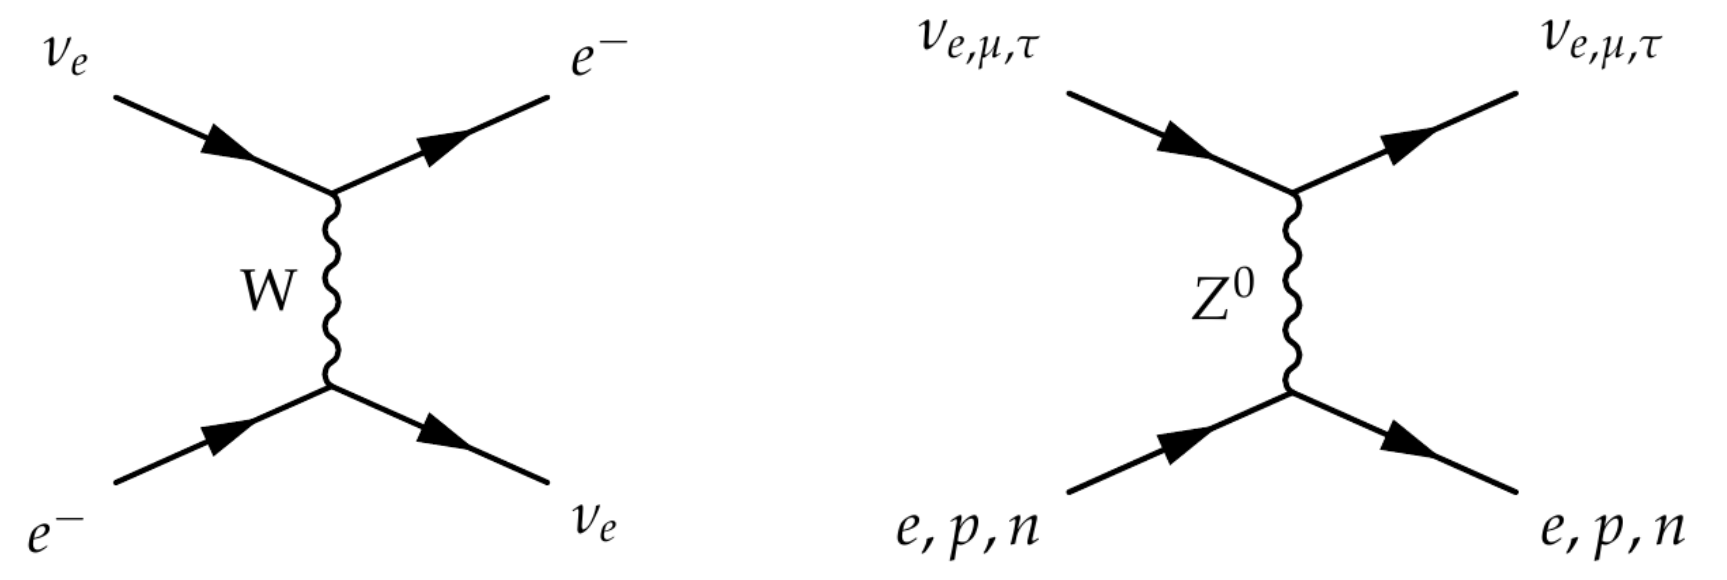
\includegraphics[width=0.8\textwidth, trim={0mm 0mm 0mm 0mm}, clip,page=1]{figures/theory/msw_effect}
%	\caption{Interaction diagrams with matter for different neutrino flavours}
%	\label{fig:msw_effect}
%\end{figure}
\begin{figure}[h]
	\begin{subfigure}[t]{0.32\textwidth}
		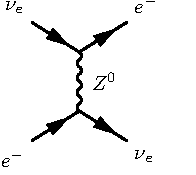
\includegraphics[width=0.8\textwidth, clip,page=1]{figures/theory/feynmp_crop}
		\caption{$\nu_e$ on $e^-$}
	\end{subfigure}
	\begin{subfigure}[t]{0.32\textwidth}
		\includegraphics[width=0.8\textwidth, clip,page=3]{figures/theory/feynmp_crop}
		\caption{$\nu_{e,\mu,\tau}$ on $e,p,n$}
	\end{subfigure}
	\begin{subfigure}[t]{0.32\textwidth}
		\includegraphics[width=0.8\textwidth, clip,page=2]{figures/theory/feynmp_crop}
		\caption{$\bar{\nu}_e$ on $e^-$}
	\end{subfigure}
	\caption{Interaction diagrams with matter for different neutrino flavours, highlighting (anti-)electron neutrino differences giving rise to different matter-effects for (anti-)electron neutrinos.}
	\label{fig:msw_effect}
\end{figure}

Electron neutrinos experience a modified Hamiltoninan potential $\Delta V = \pm 2\sqrt{2}G_F E_\nu N_e$, where $G_F$ is the Fermi constant, $E_\nu$ is the neutrino energy and $N_e$ is the electron number density of the matter, where the neutrino(anti) picks up the positive(negative) term. The effect modifies the oscillation probability to have stronger dependence on $\sin \left(\ldots \Delta m^2 \ldots \right)$, hence the sign of $\Delta m^2$ can be resolved when significant matter interactions occur\cite{msw_summary}.

\section{Neutrino Interactions}
\label{sec:theory:int}
Our limited knowledge of neutrino-matter interactions make them a dominant systematic for current long-baseline, intermediate energy neutrino oscillation experiments. The parametrisation of neutrino interaction systematics for this thesis is given in \autoref{subsec:syst_xsec}, with an overview provided here. Detailed discussions can be found in \cite{katori_martini,ulrich_review,nieves_review}.

Generally, the $E_\nu \sim 0.5-5\text{ GeV}$ regime is referred to as the ```intermediate energy region''. Neutrino-matter interactions in this region involve a range of complex nuclear physics, in which the neutrino can interact with the entire nucleus (e.g. coherent\cite{Berger_Sehgal_coh} or giant resonance\cite{crpa} interactions), nucleon pairs, single bound nucleons, and quarks (as in DIS). At the low end of the energy range, additional nuclear effects such as nucleon-nucleon correlations\cite{nieves1,nieves2}, $\Delta$ baryon in-medium modifications\cite{nuclear_effects_1pi}, $W$-boson self-energy corrections\cite{nieves1}, and nucleus spectral functions \cite{benhar}, are important. The high-end of the region is dominated by deep inelastic scattering (DIS), with dependence on parton distribution functions. The transition regions between producing no, single and multiple pions is particularly poorly modelled\cite{katori_martini,ulrich_review,nieves_review}. Neutrino-nucleus and nucleon scattering theory is often inspired by results from electron scattering experiments\cite{joanna}, such as CLAS\cite{clas} at JLAB. The electron scattering experiments have the benefit of a very narrow beam energy spectrum, so can study nuclear effects at specific $Q=P_{in}-P_{out}$ to the nucleus---unachievable with current neutrino sources.

In Monte Carlo event generators, the neutrino interaction process is commonly factorised into four parts: 1) A nucleon is simulated from a nuclear model and is used as a target for the neutrino interaction and we boost into its rest-frame, 2) The neutrino interacts with chosen nucleon which is now at rest, equivalent to a neutrino-nucleon interaction, 3) The outgoing particles from the fundamental vertex are propagated through the nucleus with radiative and final state interactions applied, 4) The particles are boosted back into the lab frame.

The total cross-sections in $E_\nu$, $\sigma(E_\nu)$, for the NEUT 5.3.3\cite{neut} generator used by T2K are shown in \autoref{fig:neut_xsecs}. At T2K energies ($E_\nu\sim0.6\text{ GeV}$) the primary interaction mode is CCQE. Charged pion production becomes important at $E_\nu\sim1\text{ GeV}$, and multi-$\pi$ and DIS above $E_\nu\sim2.5\text{ GeV}$. Since this analysis aims to minimise systematics for oscillation analyses---which select the charged-current 0$\pi$ final state at SK---the 0$\pi$ systematics have the largest impact.
\begin{figure}[h]
	\centering
	\begin{subfigure}[t]{0.42\textwidth}
		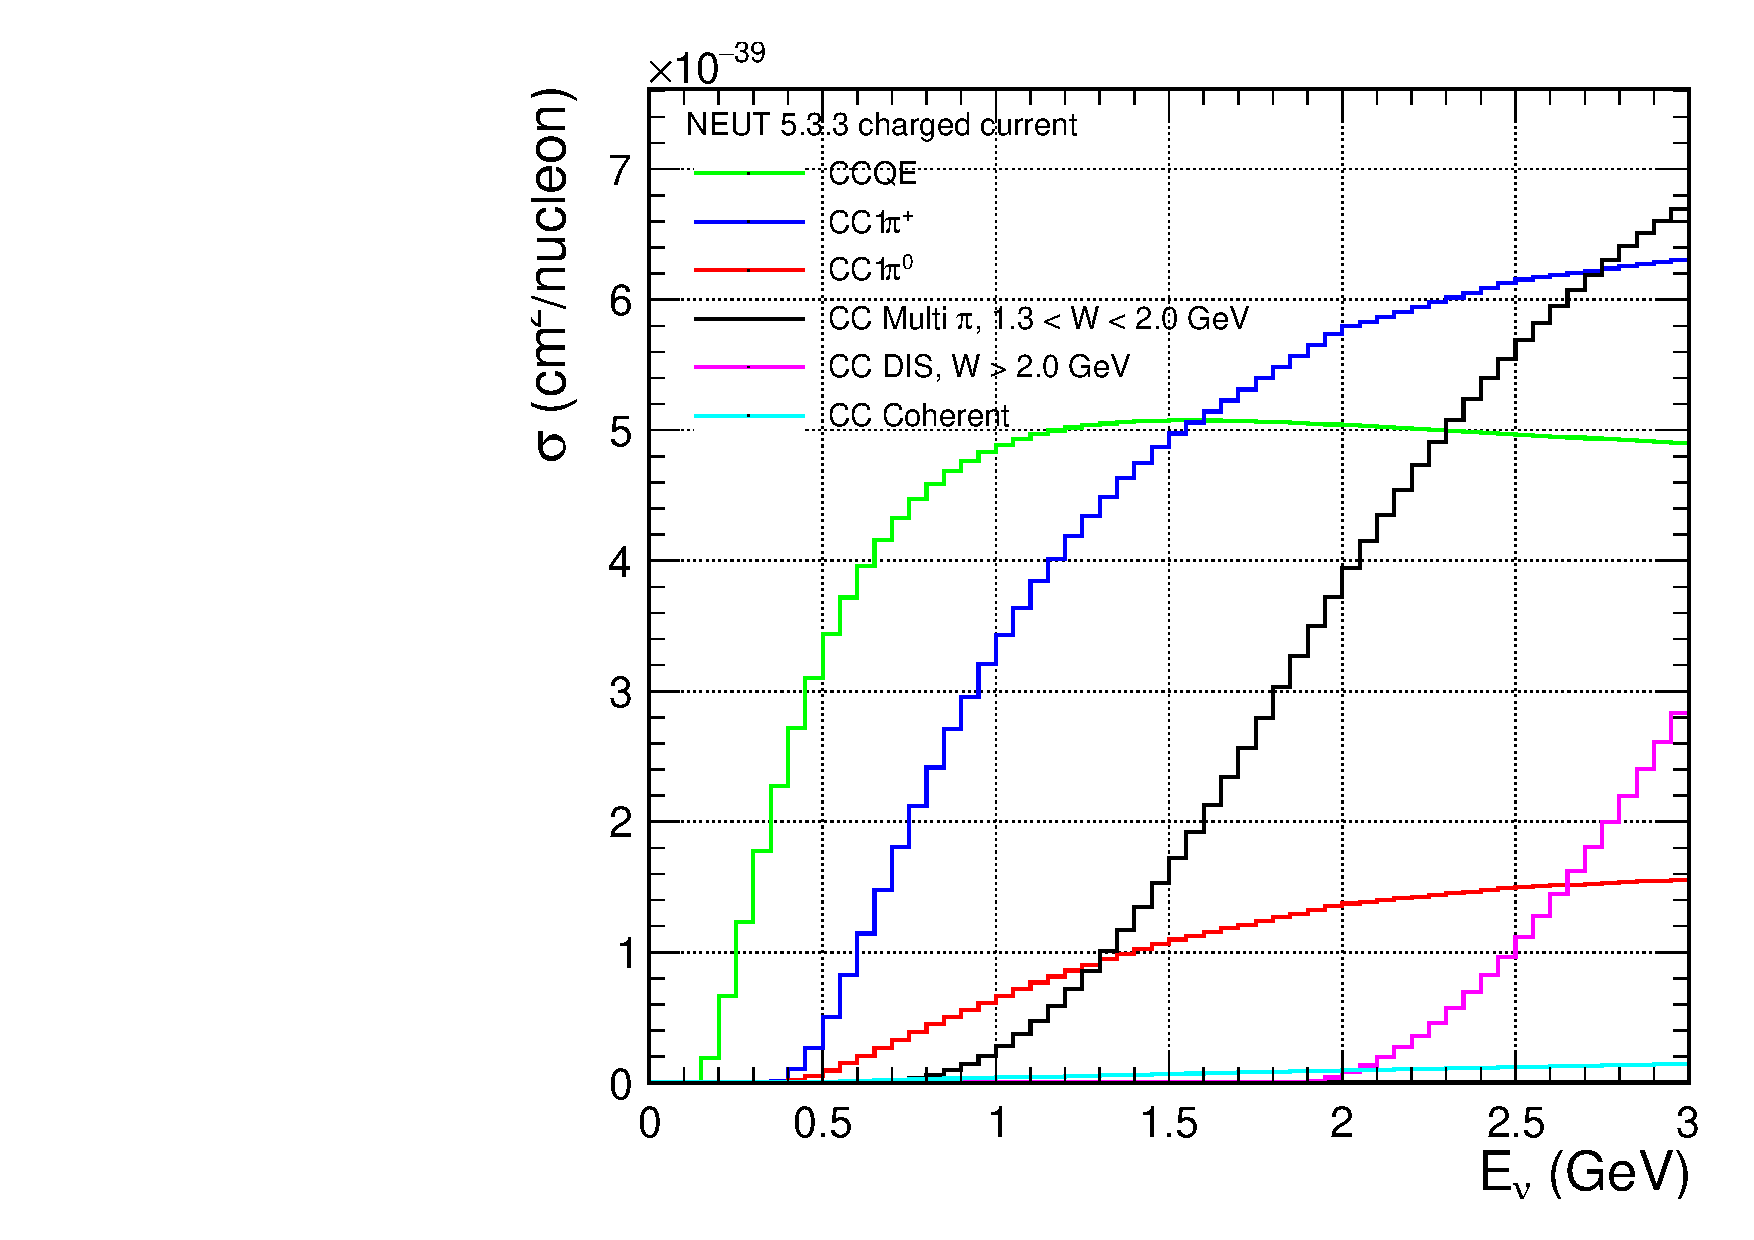
\includegraphics[width=\textwidth, trim={0mm 0mm 0mm 0mm}, clip,page=1]{figures/niwg/NEUT_533_xsecs}
		\caption{Charged current}
	\end{subfigure}
	\begin{subfigure}[t]{0.42\textwidth}
		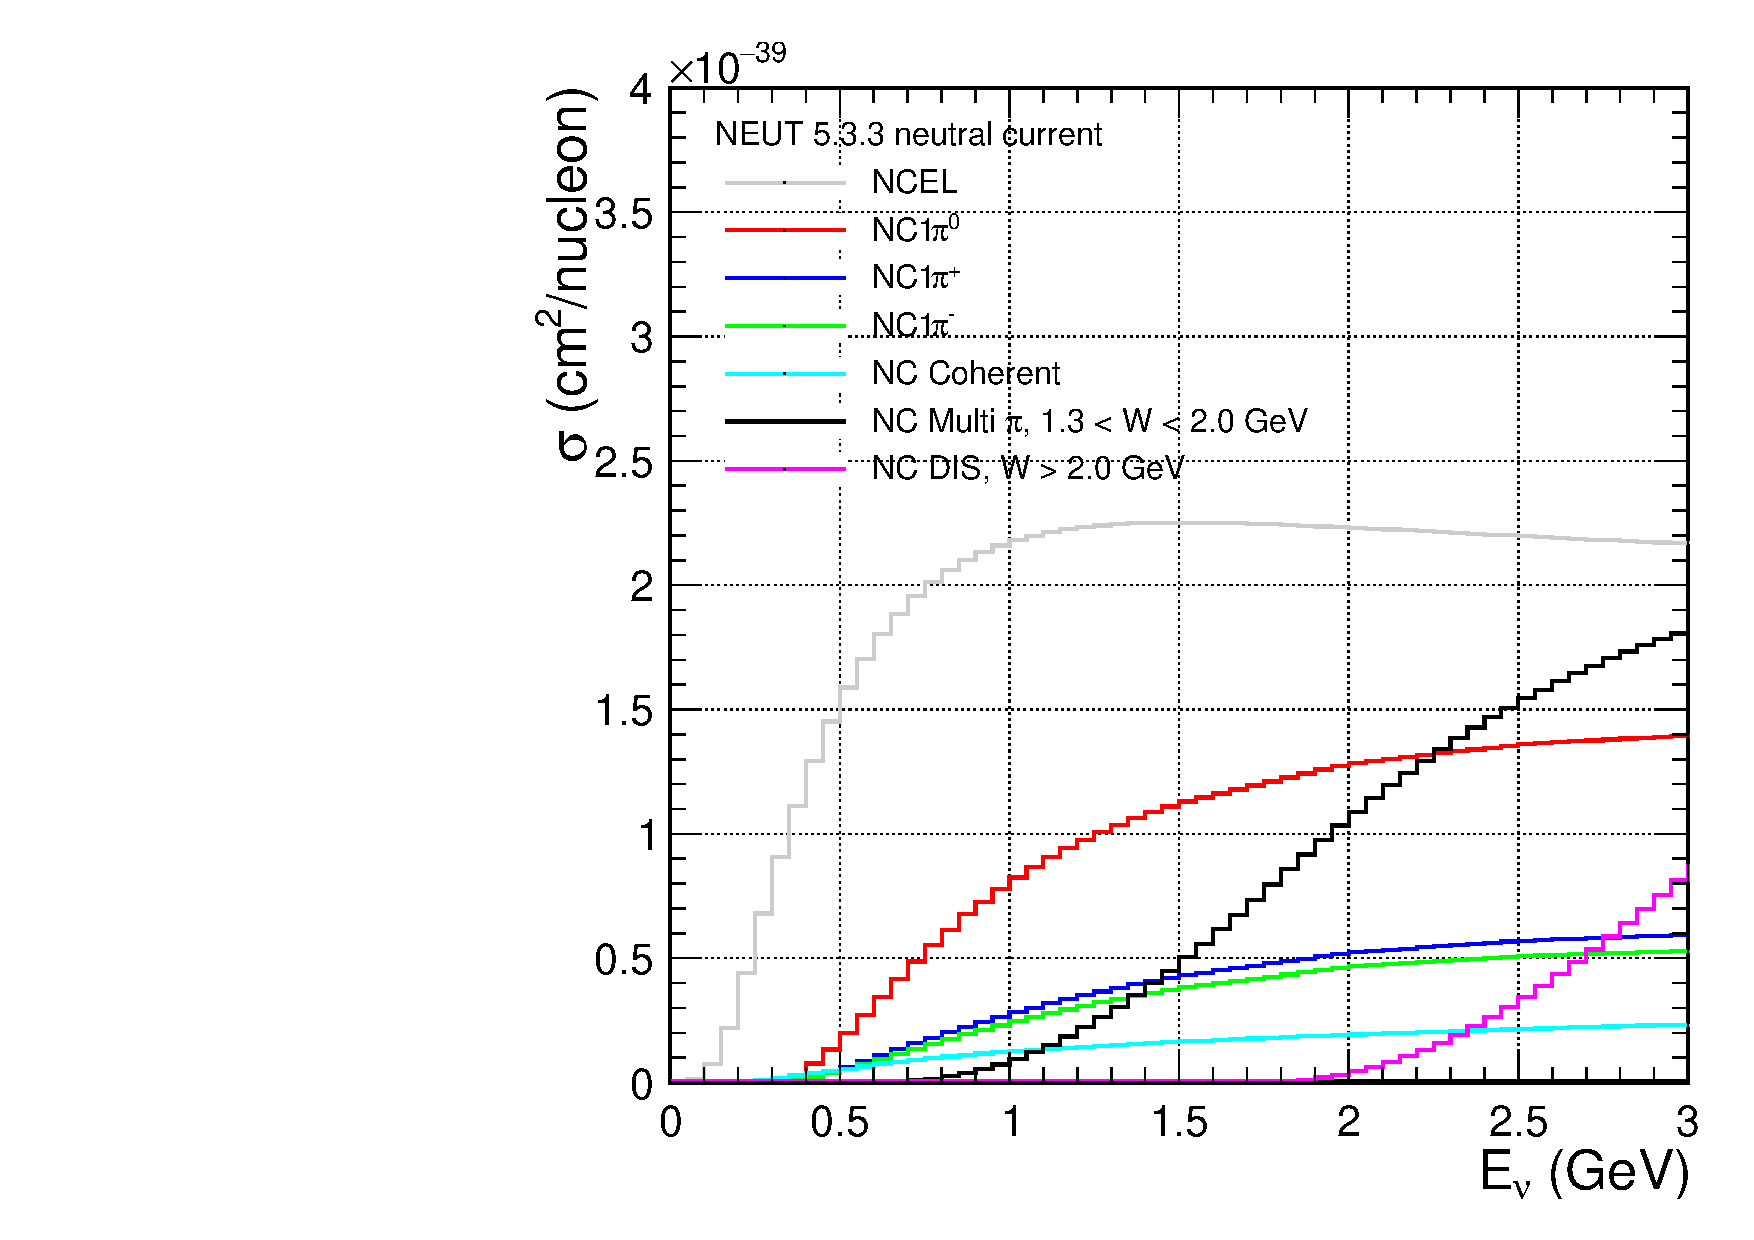
\includegraphics[width=\textwidth, trim={0mm 0mm 0mm 0mm}, clip,page=1]{figures/niwg/NEUT_533_xsecs_NC}
		\caption{Neutral current}
	\end{subfigure}
	\caption{Total cross-sections from the NEUT 5.3.3\cite{neut} neutrino interaction generator}
	\label{fig:neut_xsecs}
\end{figure}

\subsection{CC0$\pi$}
\autoref{fig:cc0pi_diag} shows some pseudo diagrams of the definition of the 0$\pi$, CCQE and one 2p2h process. The CC0$\pi$ signal definition does not include hadronic information, so the CCQE and 2p2h processes both produce 0$\pi$ final states. T2K uses the CCQE diagram for neutrino energy reconstruction, assuming a nucleon at rest. If 2p2h events are included in the selection it biases $E_\nu$, and wrongly estimating the bias has a noticeable effect on oscillation parameters. The same holds true for including single pion events due to unreconstructed pions or final state interactions.
\begin{figure}[h]
	\centering
	\begin{subfigure}[t]{0.32\textwidth}
		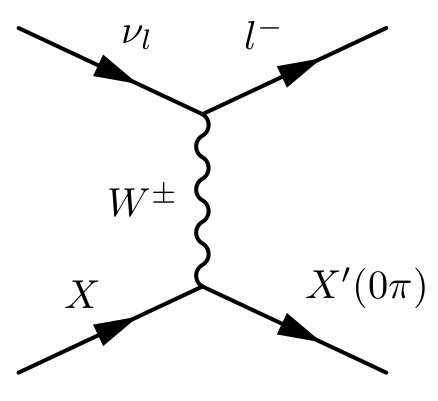
\includegraphics[width=\textwidth, trim={0mm 0mm 0mm 0mm}, clip,page=1]{figures/niwg/diagrams/CC0pi}
		\caption{CC0$\pi$, defined as having an outgoing charged lepton and no charged or neutral pions}
	\end{subfigure}
	\begin{subfigure}[t]{0.32\textwidth}
		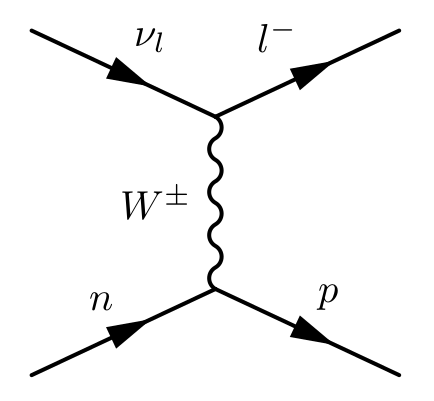
\includegraphics[width=\textwidth, trim={0mm 0mm 0mm 0mm}, clip,page=1]{figures/niwg/diagrams/CCQE}
		\caption{CCQE, defined as having interacted on an initial state neutron, producing an outgoing charged lepton and proton}
	\end{subfigure}
	\begin{subfigure}[t]{0.32\textwidth}
		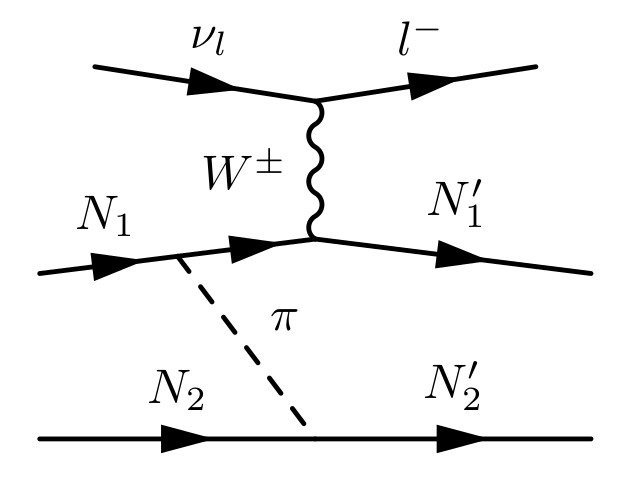
\includegraphics[width=\textwidth, trim={0mm 0mm 0mm 0mm}, clip,page=1]{figures/niwg/diagrams/2p2h_possibly}
		\caption{One of many 2p2h processes, defined as an interaction on two initial state nucleons which are coupled}
	\end{subfigure}
	\caption{CC0$\pi$, CCQE and 2p2h pseudo-diagrams}
	\label{fig:cc0pi_diag}
\end{figure}

Generally, the neutrino-nucleon CCQE interaction is relatively well understood. The current effort in the field is to understand the impact of form factor choices, numerous nuclear effects, and minimising the models' impacts on cross-section and oscillation measurements.

\subsection{Single Pion Production}
\autoref{fig:1pi_diags} shows the dominant charged-current neutrino-nucleon interactions giving rise to single pion production (SPP). The interaction proceeds by a resonant state here labelled as $\Delta$, which is dominant at T2K energies. SPP makes up $\sim20\%$ of selected 0$\pi$ events at SK due to missing pions.
\begin{figure}[h]
	\centering
	\begin{subfigure}[t]{0.32\textwidth}
		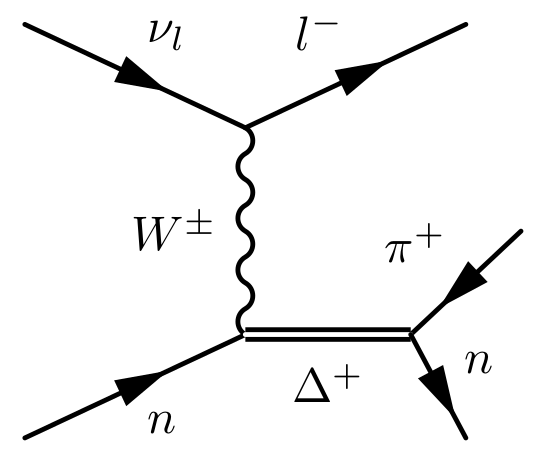
\includegraphics[width=\textwidth, trim={0mm 0mm 0mm 0mm}, clip,page=1]{figures/niwg/diagrams/CC1npip}
		\caption{CC1$\pi^+$1n}
	\end{subfigure}
	\begin{subfigure}[t]{0.32\textwidth}
		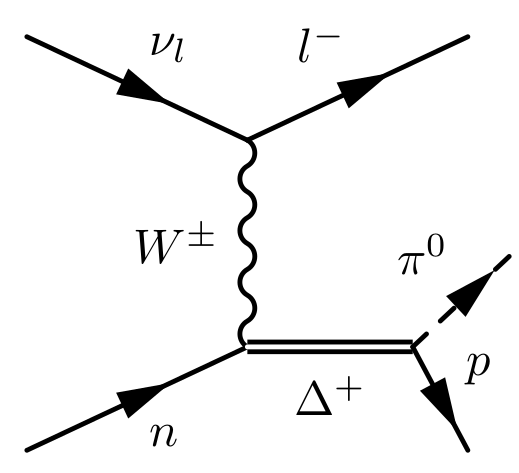
\includegraphics[width=\textwidth, trim={0mm 0mm 0mm 0mm}, clip,page=1]{figures/niwg/diagrams/CC1pi0}
		\caption{CC1$\pi^0$}
	\end{subfigure}
	\begin{subfigure}[t]{0.32\textwidth}
		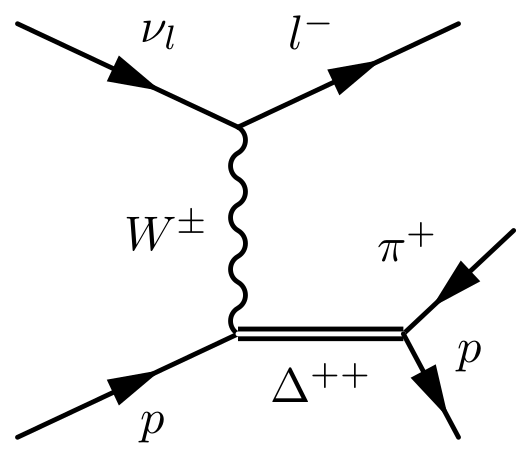
\includegraphics[width=\textwidth, trim={0mm 0mm 0mm 0mm}, clip,page=1]{figures/niwg/diagrams/CC1ppip}
		\caption{CC1$\pi^+$1p}
	\end{subfigure}
	\caption{Charged-current single pion production on a nucleon via a $\Delta$ resonance}
	\label{fig:1pi_diags}
\end{figure}

Contrary to the CCQE interaction, single pion production on free nucleons is poorly modelled. The low hadronic mass $(W)$ regime where the single $I_{3/2}$ $\Delta^{++}\rightarrow p+\pi^+$ interaction dominates can be considered understood, although resonance-resonance and resonance-non-resonance interference present at higher $W$ is not. Additionally, in-medium effects from resonance fields propagating the nucleus are poorly understood and multi-nucleon couplings often unmodelled\cite{nustec,katori_martini}.

\subsection{Multi-$\pi$ and DIS}
The transition from SPP to DIS is generally referred to as soft inelastic scattering (SIS). NEUT uses a custom interpolation between $1.3 < W < 2.0 \text{GeV}$, selecting events with $N_\pi>1$ to avoid double counting SPP cross-sections. Other generators such as GENIE\cite{genie} and NuWro\cite{NuWro} use different implementations. A pseudo diagram is shown in \autoref{fig:dis_diags}, where fragmentation causes the pion emissions.

\subsection{Subdominant Interactions}
Subdominant interactions with small interaction cross-sections can populate very specific signal regions, e.g. NC$1\gamma$ and NC1$\pi^0$ mimicking $\nu_e + X\rightarrow e^- + X'$, and differences in $\nu_e$ vs $\nu_\mu$. Historically, there is much less cross-section data on NC interactions than CC and barely any using electron neutrinos, and it is common to trust model extrapolation from CC to NC rather than test against data. 

The charged current coherent process shown in \autoref{fig:coh_diags} occupies a very specific phase space: the very forward going, collinear lepton-pion, low $Q^2$ region. This is important since it has the same final state as single pion production, although not produced through a resonance, making up about 10\% of the most forward-going \cosmu bin in CC1$\pi$ selections.
\begin{figure}[h]
	\centering
	\begin{subfigure}[t]{0.42\textwidth}
		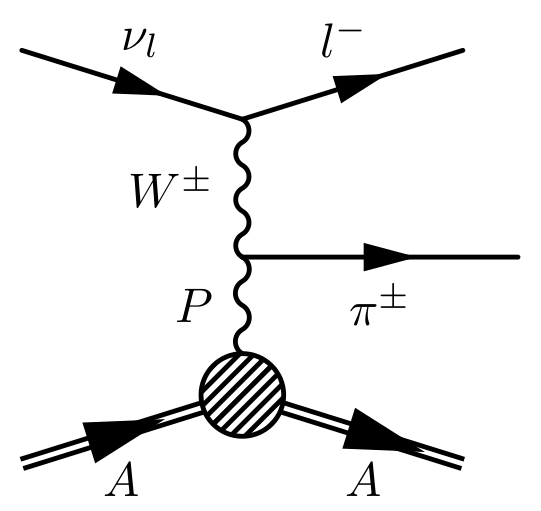
\includegraphics[width=\textwidth, trim={0mm 0mm 0mm 0mm}, clip,page=1]{figures/niwg/diagrams/CCcoh}
		\caption{CC coherent}
		\label{fig:coh_diags}
	\end{subfigure}
	\begin{subfigure}[t]{0.42\textwidth}
		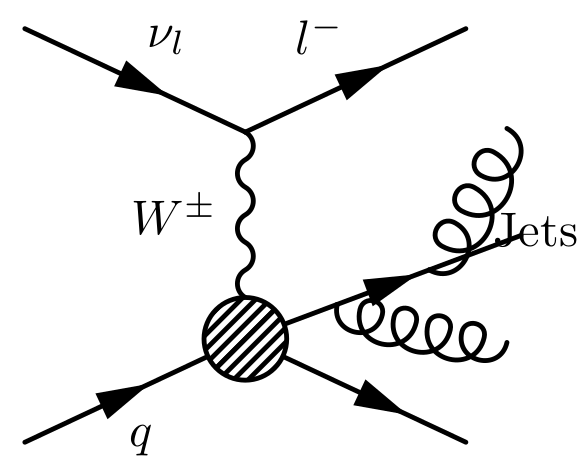
\includegraphics[width=\textwidth, trim={0mm 0mm 0mm 0mm}, clip,page=1]{figures/niwg/diagrams/CCmultipion}
		\caption{CC DIS}
		\label{fig:dis_diags}
	\end{subfigure}
	\caption{Coherent and multi-pion/DIS scattering diagrams}
	\label{fig:coh_dis_diags}
\end{figure}

\subsection{Intranuclear Hadronic Cascades}
The nuclear cascade following the initial neutrino-nucleon interaction is handled by a microscopic hadron propagation in NEUT. The hadron interaction probabilities are re-calculated as the hadron travels through the nucleus, seen in \autoref{fig:fsi_cascade}. 

Simulations can be considered to agree relatively well with pion scattering data\cite{thesis_elder}, but there are concerns that extrapolating results into the neutrino-nucleus interaction is poorly justified\cite{ulrich_review}. More sophisticated models exist in the Giessen-Boltzmann-Uehling-Uhlenbeck (GiBUU)\cite{gibuu} generator, although its role as a primary generator in neutrino physics is currently unviable due to computational requirements.
\begin{figure}[h]
	\centering
	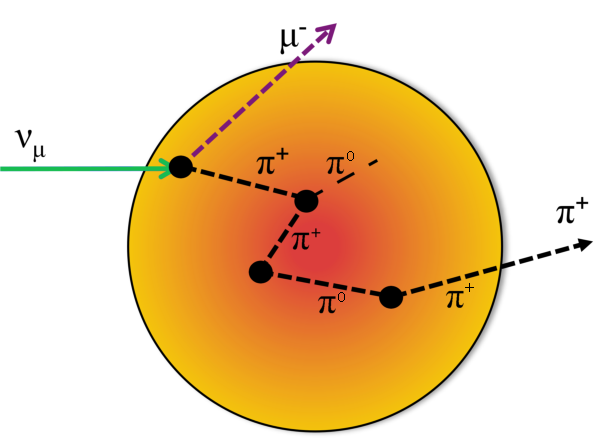
\includegraphics[width=0.3\textwidth, trim={0mm 0mm 0mm 0mm}, clip,page=1]{figures/niwg/diagrams/cascade}
	\caption{An example of a pion FSI cascade}
	\label{fig:fsi_cascade}
\end{figure}

\section{Experimental Overview}
\label{sec:exp_overview}
Neutrino oscillations is now an established physics phenomenon, cemented by awarding the 2015 Nobel Prize in Physics to Kajita-san (SK) and Art McDonald (SNO) for their experiments' measurements of solar and atmospheric neutrino oscillations. This section gives a brief introduction and overview of neutrino oscillation experiments and production mechanisms, summarised in \autoref{fig:all_neutrino_expts}. Experiments are generally categorised in neutrino energy $E$ and baseline $L$, and the combination of $L/E$ largely determines which oscillation parameter(s) an experiment has sensitivity too.
\begin{figure}[h]
	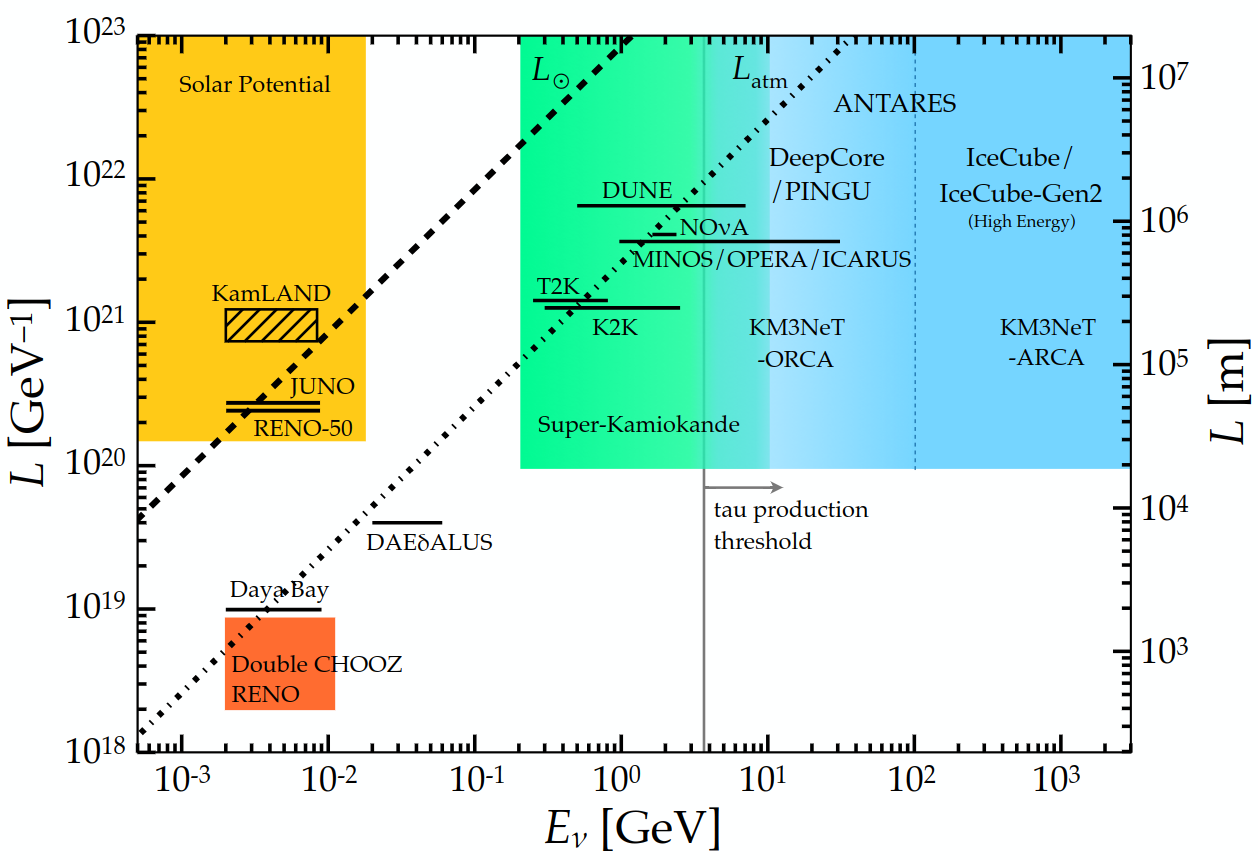
\includegraphics[width=0.7\textwidth, trim={0mm 0mm 0mm 0mm}, clip,page=1]{figures/theory/le_experiments}
	\caption{Neutrino oscillation experiments in baseline $L$ and energy $E$. Figure from \cite{ic_neutrino_2018}.}
	\label{fig:all_neutrino_expts}
\end{figure}

\subsection{Solar Neutrinos}
Solar neutrinos emanate from various nuclear fusion products and decays in the sun. \autoref{tab:solar_flux} shows the fluxes for various sources, where the $pp$ flux is strongest. However, the neutrino energy is often below threshold for the largest contributors to the flux, and most solar neutrino experiments measure the $^{8}\text{B}$ flux, shown in \autoref{fig:solar_flux}.
\begin{table}[h]
	\begin{tabular}{l | c c}
		\hline
		\hline
		Reaction & Label & Flux ($\text{cm}^{-2} \text{s}^{-1}$) \\
		\hline
		$p+p\rightarrow ^{2}\text{H} + e^+ + \nu_e$ & $pp$ & $5.95\times10^{10}$ \\
		$p+e^-+p\rightarrow ^{2}\text{H} \nu_e$ & $pep$ & $1.40\times10^{8}$ \\
		$^{3}\text{He} + p\rightarrow ^{4}\text{H} + e^+ + \nu_e$ & $hep$ & $9.3\times10^{3}$ \\
		$^{7}\text{Be} + e^- \rightarrow ^{7}\text{Li} + \nu_e$ & $^{7}\text{Be}$ & $4.77\times10^{9}$ \\
		$^{8}\text{B} \rightarrow ^{8}\text{Be}* + e^+ \nu_e$ & $^{8}\text{B}$ & $5.05\times10^{6}$ \\
		\hline
		\hline
	\end{tabular}
	\caption{Integrated solar neutrino flux from various solar processes in the $pp$ chain. Table replicated from \cite{solar_review}.}
	\label{tab:solar_flux}
\end{table}

\begin{figure}[h]
	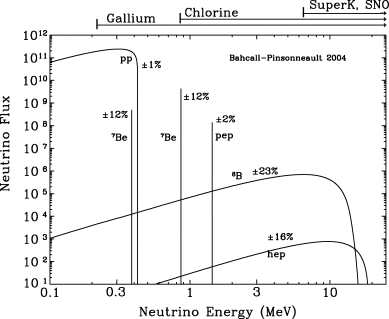
\includegraphics[width=0.5\textwidth, trim={0mm 0mm 0mm 0mm}, clip,page=1]{figures/theory/solar_flux}
	\caption{Solar flux from different solar fusion processes, including thresholds of experiments. Figure from \cite{sno_solar_flux}.}
	\label{fig:solar_flux}
\end{figure}

R. Davis and J. Bachall continued their 1964 measurements\cite{davis} of the solar neutrinos from $^{8}\text{B}$ and in 1968\cite{davis_sun} announced a solar $\nu_e$ flux a factor of seven below the expected ($\sim2\sigma$ significance), at the time attributed to inaccurate solar model calculations. This was the birth of the ``solar neutrino problem'', which Bruno Pontecorvo and Vladimir Gribov in 1969\cite{pontecorvo_gribov} proposed solving by invoking a $\nu_e\leftrightarrow\nu_\mu$ oscillation similar to $K^0 \leftrightarrow\bar{K}^0$, giving rise to the PMNS paradigm in its current form, first developed around the early 1960s. In 1989, the Kamiokande experiment\cite{kamiokande_solar} confirmed the 1968 measurements of Davis and Bachall, measuring a solar neutrino flux from $^{8}\text{B}$  of $\sim0.5$ the expected, agreeing with the higher statistics data from Homestake\cite{davis_sun2}. The solar neutrino deficit was confirmed from the low threshold detectors SAGE\cite{sage_solar} and GALLEX\cite{gallex_solar}, additionally capable of detecting $p p$ neutrinos using $^{71}\text{Ga}+\nu_e \rightarrow ^{71}\text{Ge}+e^-$.

The Sudbury Neutrino Observatory (SNO) put the nail in the coffin in 2002\cite{sno_solar} by measuring solar neutrinos from $^{8}\text{B}$ in three channels: $\nu_e + d \rightarrow p+p+e^-$ (CC), $\nu_x + d\rightarrow p+ n + \nu_x$ (NC) and $\nu_x + e^- \rightarrow \nu_x+e^-$ (ES). The measured neutrino rates had a $\nu_e$ component consistent with previous measurements, a strong non-$\nu_e$ component 5.3$\sigma$ above zero, and a NC component consistent with predictions from solar models.

Additionally, the low threshold, low background, Borexino experiment detected solar neutrinos from the $^{8}\text{B}$, $^{7}\text{Be}$, $pep$, and $pp$ processes\cite{borexino_summary}. The final stages of Borexino aims to measure the CNO cycle and the next-generation SNO+ experiment aims to confirm and improve these measurements, and make detailed measurements of the MSW effect, solar metallicity and luminosity\cite{sno_plus}.

Although the solar neutrino oscillation parameters $\Delta m^2_{21}$ and $\theta_{12}$ are considered well-constrained, there is $\sim 2\sigma$ tension on $\Delta m^2_{21}$ between the solar neutrino measurements at SK and SNO (which are internally compatible), and the long baseline reactor anti-electron-neutrino experiment, KamLAND\cite{m2_tension}, measuring the same oscillation process but with a different neutrino source.

\subsection{Atmospheric Neutrinos}
Atmospheric neutrinos are emitted when cosmic rays interact with nuclei in the earth's atmosphere, producing mesons which decay into neutrinos, amongst other particles. The primary decay is the pion decay,
\begin{gather*}
	\pi^\pm \rightarrow \mu^\pm + \nu_\mu(\bar{\nu}_\mu) \\
	\mu^\pm \rightarrow e^\pm + \bar{\nu}_\mu (\nu_\mu) + \nu_e (\bar{\nu}_e)
\end{gather*}
giving rise to a total of three neutrinos. The atmospheric neutrino flux calculations from Honda\cite{honda_flux} is shown in \autoref{fig:atmos_flux}, which peaks in the 1-10 GeV region, notably higher than the solar neutrinos.
\begin{figure}[h]
	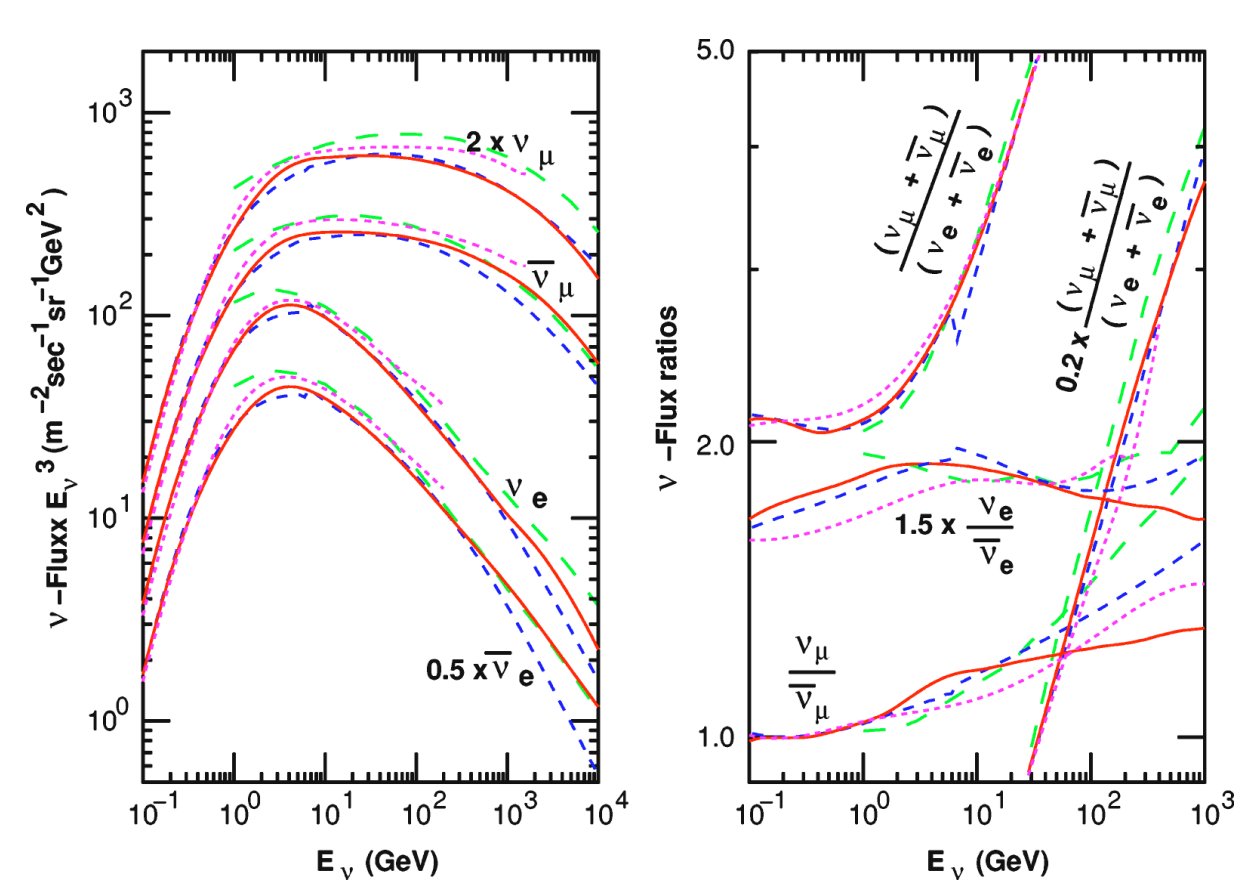
\includegraphics[width=0.7\textwidth, trim={0mm 0mm 0mm 0mm}, clip,page=1]{figures/theory/honda_flux}
	\caption{Atmospheric neutrino flux from Honda et al. \cite{honda_flux}.}
	\label{fig:atmos_flux}
\end{figure}

In 1965 F. Reines\cite{reines_atmos} and C.V. Achar\cite{india_atmos_hint} first saw hints of atmospheric $\nu_\mu$ disappearance in deep underground laboratories through $\nu_\mu(\bar{\nu}_\mu) + X \rightarrow \mu^\pm + X'$. The Irvine-Michigan-Brookhaven (IMB) experiment observed deficits of $\nu_\mu$ interactions in 1986\cite{imb}, and Kamiokande II in 1988\cite{kamiokande_atmos_hint} verified this and found muon-like events of $59\pm7\%$ the prediction, although good agreement of electron-like single-prong events. The Soudan-2 experiment\cite{soudan2} also saw muon neutrino deficiency with a flavour ratio of $0.72\pm0.19^{+0.05}_{-0.07}$ relative the expectation. 

When SK in 1998 published\cite{sk_disc} their high-statistics\footnote{4353 fully-contained and 301 partially-contained events} $\nu_\mu$ data, they found $R=\left( \mu/e \right)_\text{Data}/\left( \mu/e \right)_\text{MC} =0.65\pm0.05\pm0.08$. They additionally fitted the oscillation parameters, finding the data well described by $\nu_\mu \leftrightarrow \nu_\tau$ rather than $\nu_\mu \leftrightarrow \nu_e$ oscillations. The summary of flavour ratios for atmospheric neutrinos is seen in \autoref{fig:atmos_ratio}, where the majority of the high precision data sits at $R=0.5-0.8$.
\begin{figure}[h]
	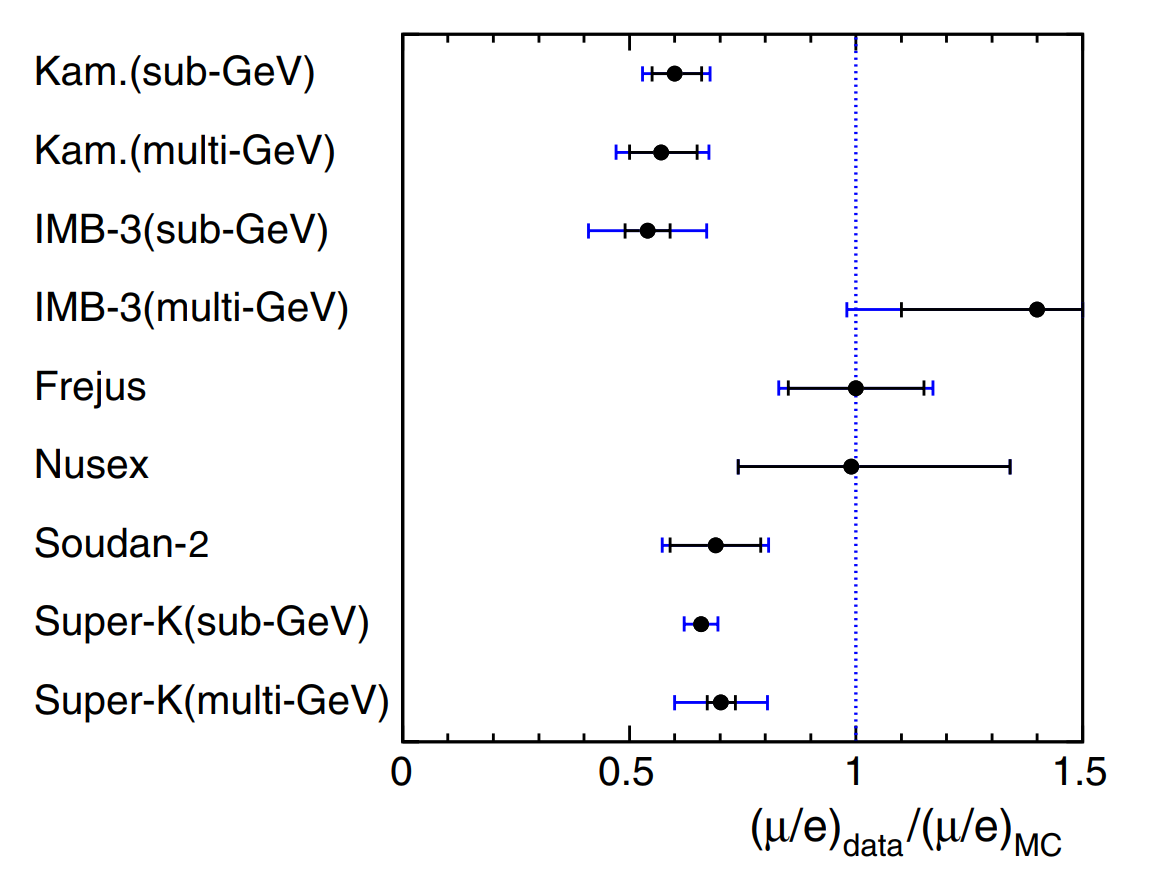
\includegraphics[width=0.7\textwidth, trim={0mm 0mm 0mm 0mm}, clip,page=1]{figures/theory/flavour_ratio}
	\caption{Measured flavour ratios for various historic atmospheric neutrino experiments, showing consistent under-prediction of the $\mu/e$ ratio in data and simulation. Figure from \cite{kajita_summary}.}
	\label{fig:atmos_ratio}
\end{figure}

Atmospheric neutrino observatories after the mid 2000s have focussed on measuring $\nu_\mu\rightarrow\nu_\mu$ with increasing precision. Furthermore, by isolating regions of specific zenith angle (and therefore baseline $L$), the extent of the matter effects are also studied, which may resolve the ordering of the mass states. This is largely the focus of the atmospheric neutrino programmes at IceCube\cite{icecube}, ANTARES\cite{antares}, SNO \cite{sno_atmos} and SK\cite{superk}. The latter has also made attempts at isolating $\nu_\tau$ events\cite{superk_tau}, claiming $4.6\sigma$ discovery of $\nu_\tau$ appearance in 2017. A summary of some recent results including complementary long baseline accelerator neutrino experiments can be seen in \autoref{fig:atmos_data}.
\begin{figure}[h]
	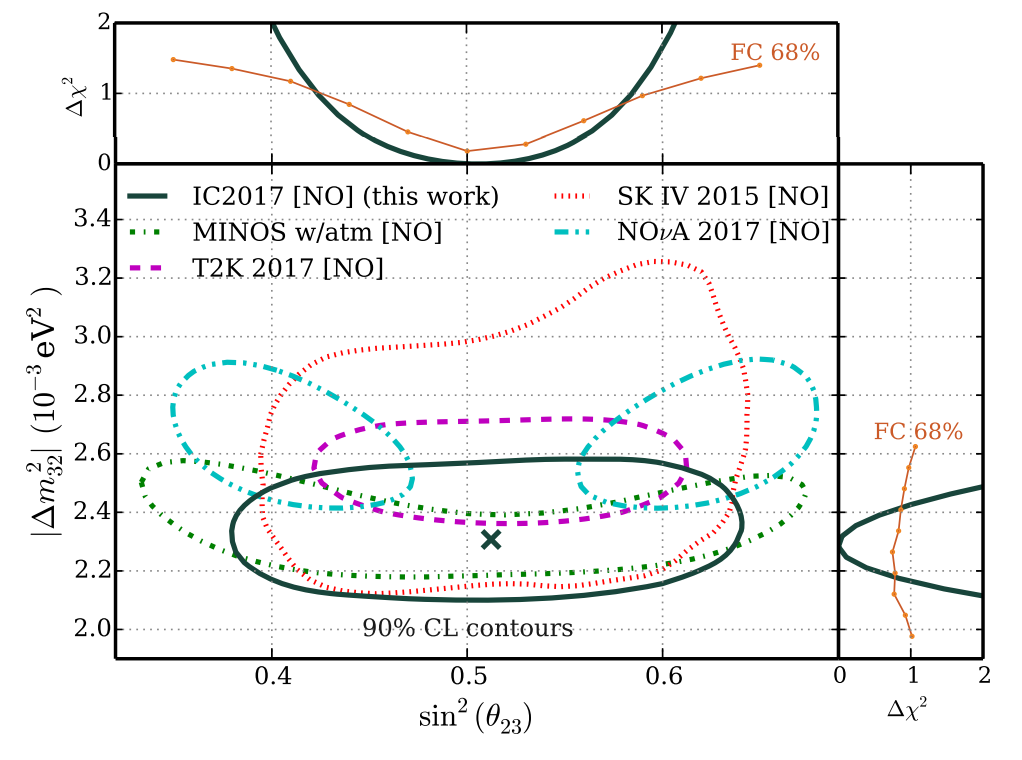
\includegraphics[width=0.7\textwidth, trim={0mm 0mm 0mm 0mm}, clip,page=1]{figures/theory/icecube_comp}
	\caption{Measured atmospheric oscillation parameters from recent atmospheric and long baseline accelerator neutrino experiments, assuming normal ordering. Figure from \cite{icecube}.}
	\label{fig:atmos_data}
\end{figure}

\subsection{Accelerator Neutrinos}
Accelerator neutrino experiments are similar to atmospheric experiments in neutrino energy, baseline and the neutrino source's production mechanism. The neutrinos are made by impinging protons from accelerators on targets, producing a flurry of mesons which typically decay into muon flavoured neutrinos, amongst others. Experiments often have the ability to deflect and/or focus mesons after the target, enabling sign selection and thus $\nu_\mu$ and $\bar{\nu}_\mu$ selection. In contrast to atmospheric neutrinos, accelerator neutrinos are about 90\% muon flavoured.

The atmospheric neutrino oscillations, outlined earlier, became the driver behind the accelerator programme in the late 1990s. Since the neutrino energy and baseline can be tuned and chosen in an accelerator experiment, the oscillation dip suggested by atmospheric neutrino experiments can be bombarded with statistics. Furthermore, the dependence on the atmospheric flux simulation is removed\cite{lbnl_review}. The disadvantage is the reduced total flux at the far-detector, generally forcing the baseline to $L<1000\text{ km}$, which limits the impact of the matter effect and sensitivity to the mass ordering. The majority of long baseline accelerator neutrino experiments include a near detector which samples the beam before any long baseline oscillations have taken place.

The short-baseline ($L\sim 1\text{ km}$) accelerator neutrino experiments, such as MiniBooNE\cite{mb_design}, MINER$\nu$A\cite{minerva_design}, and the upcoming SBND programme\cite{sbnd}, are generally intended to measure neutrino cross-sections and perform short baseline oscillation searches. They may also serve as neutrino beam monitors for other experiments. The interaction measurements are used to inform neutrino event generators\cite{neut,genie,NuWro}, aiding in informing systematic uncertainties for neutrino cross-section and oscillation experiments.

The pioneering long-baseline ($L\sim 100-1000\text{ km}$) experiments MINOS\cite{minos_obs} and K2K\cite{k2k_obs} confirmed the atmospheric neutrino mixing in $\nu_\mu \rightarrow \nu_\mu$, finding compatible oscillation parameters. The searches for $\nu_\mu \rightarrow \nu_e$ at K2K and MINOS were not statistically significant\cite{k2k_noobs,minos_disc} and were discovered by the next generation experiments T2K\cite{t2k_disc} and \nova\cite{nova_disc}, with evidence of the $\bar{\nu}_\mu \rightarrow \bar{\nu}_e$ oscillation presented by \nova at Neutrino 2018\cite{nova_neutrino2018}. The Japanese experiments K2K and T2K have consistently used the 50,000 tonne water Cherenkov detector SK\cite{superk} as the far detector, with plastic scintillator based near-detectors and a baseline of $L\sim250-300\text{ km}$ and $E\sim0.5-2\text{ GeV}$. Both MINOS and \nova, with $L\sim700\text{ km}$ and $E\sim2-5\text{ GeV}$, use(d) purpose-built functionally identical near and far-detectors, allowing for many uncertainties from systematic parameters to be reduced significantly.

In Europe, the OPERA\cite{opera} experiment was designed to look for the dominant $\nu_\mu \rightarrow \nu_\tau$ oscillation at $L\sim700\text{ km}$. The ICARUS\cite{icarus} experiment searched for $\nu_\mu\rightarrow\nu_e$ from a fourth ``sterile'' neutrino, observed by LSND\cite{lsnd} and MiniBooNE\cite{miniboone_sterile} which has been questioned by the community\cite{lsnd_refute}. The detection threshold for the charged current interaction $\nu_\tau + X \rightarrow \tau + X'$ is $E_\nu\sim 3.5\text{ GeV}$, so the neutrino beam from CERN to Gran Sasso (CNGS)\cite{cngs} was wide-band with $E_\nu = 10-25\text{ GeV}$. The $\tau$ detection requires very fine granularity and OPERA used nuclear emulsions whereas ICARUS pioneered the use of liquid argon TPCs in neutrino physics. OPERA measured $\nu_\tau$ appearance\cite{opera_final_tau} at 6.1$\sigma$, and both OPERA and ICARUS found no evidence of sterile neutrinos\cite{icarus_lsnd,opera_lsnd}.

\subsection{Reactor Anti-Electron Neutrinos}
Reactor neutrinos are formed in $\beta$ decay of fission products in nuclear reactors, e.g. $^{231}\text{Th} \rightarrow ^{231}\text{Pa} + e^- + \bar{\nu}_e$ and $^{215}\text{Po} \rightarrow ^{211}\text{Pb} + e^- + \bar{\nu}_e$. The neutrino flux depends on the relative fission yields of the products, but generally has a similar energy spectrum to solar neutrinos, in the 1-10 MeV range. The $\bar{\nu}_e$ flux from a test reactor is shown in \autoref{fig:reactor_flux}.
\begin{figure}[h]
	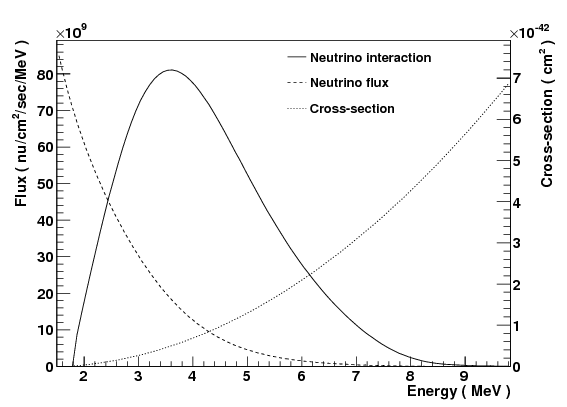
\includegraphics[width=0.6\textwidth, trim={0mm 0mm 0mm 0mm}, clip,page=1]{figures/theory/reactor_flux}
	\caption{Reactor flux for the Japanese experimental fast reactor, JOYO. Figure from \cite{reactor_flux}.}
	\label{fig:reactor_flux}
\end{figure}

Reactor anti-electron neutrinos are exclusively detected by the IBD interaction, in which the $e^+ + e^- \rightarrow 2\gamma$ annihilation photons are measured in scintillator. Many experiments additionally dope or surround the scintillator with a high neutron capture element (e.g. $^{6}\text{Li}$ or $^{157}\text{Gd}$). In the case of Gd doping, the signal consists of the prompt $2\gamma$ followed by a $\sim30\mu\text{s}$ delayed $\gamma$ cascade with $E_\gamma^{tot}\sim8\text{ MeV}$ from the Gd de-excitation, facilitating signal-background separation\cite{daya_bay,reno}.

Similar to accelerator neutrino experiments, the reactor experiments can be categorised by baseline. Short baseline experiments with $L\sim1-2\text{ km}$ perform world-leading measurements of $|\Delta m^2_{13}|$ and $\sin^2\theta_{13}$ and probe parts of the sterile neutrino spectrum. Daya Bay\cite{daya_bay_disc}, RENO\cite{reno_disc} and Double Chooz\cite{double_chooz} all measured a relatively large $\sin^2 \theta_{13}$, enabling $\nu_e$ appearance to be observed at long baseline neutrino experiments such as T2K and \nova. The short baseline reactor results on $\sin^2\theta_{13}$ are often used in atmospheric and accelerator oscillation analyses for increased sensitivity to the 2,3 parameters, the mass ordering, and $\delta_{CP}$. A summary plot of the measured neutrino oscillation parameters by short baseline reactor and long baseline accelerator neutrino oscillation experiments is shown in \autoref{fig:13_sector}.
\begin{figure}[h]
	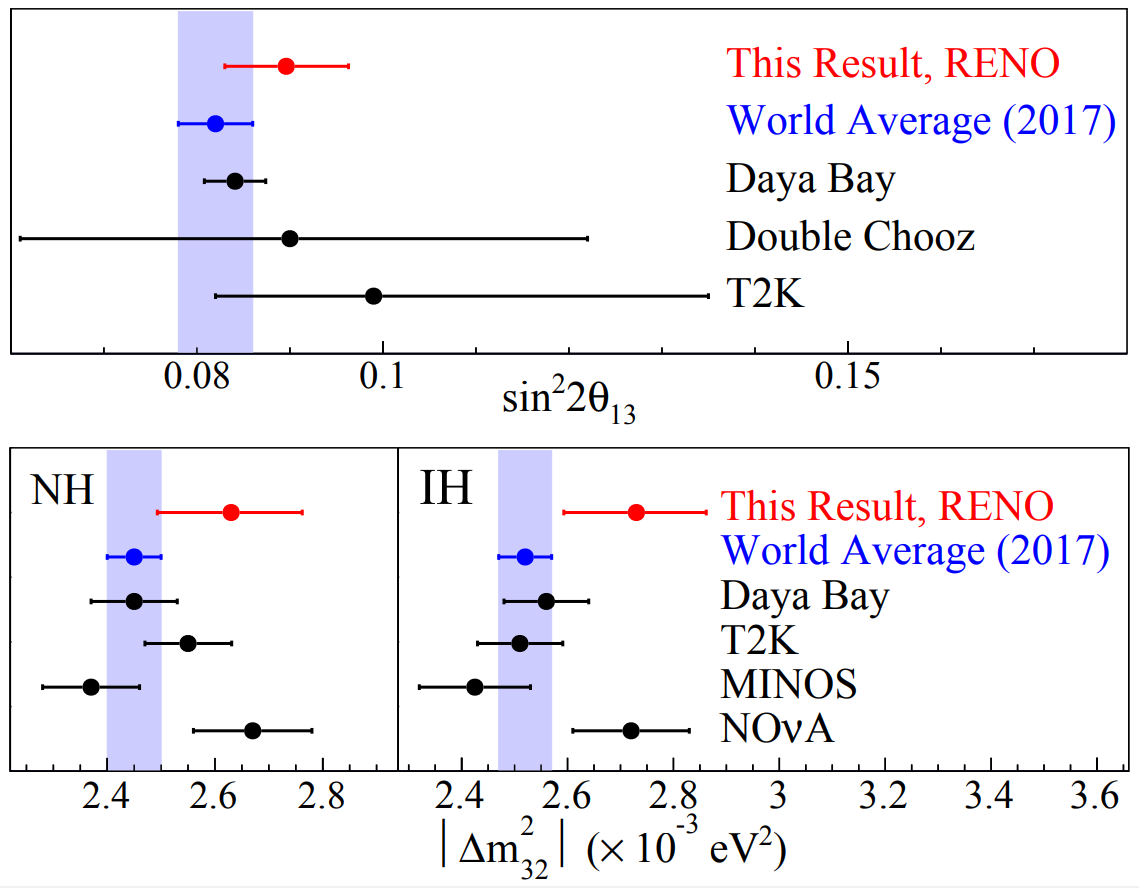
\includegraphics[width=0.6\textwidth, trim={0mm 0mm 0mm 0mm}, clip,page=1]{figures/theory/reno_theta_dm13}
	\caption{$\Delta m^2_{23}$ and $\sin^2 2\theta_{13}$ measurements from reactor (Daya Bay\cite{daya_bay}, RENO\cite{reno_new} and Double Chooz\cite{double_chooz_old}) and accelerator (T2K\cite{t2k_2015}, \nova\cite{nova_2017} and MINOS\cite{minos_numu_nue}) neutrinos. Figure from \cite{reno_new}.}
	\label{fig:13_sector}
\end{figure}

The only medium baseline experiment ($L\sim50\text{ km}$) is JUNO\cite{juno}, currently under construction in China. It aims to measure the neutrino mass ordering by separating the oscillations into fast and slow parts from $\Delta m^2_{23}$ and $\Delta m^2_{12}$, and improve measurements of $\sin^2 \theta_{12}$.

The Japanese KamLAND experiment is the only long baseline ($L\sim180\text{ km}$) reactor anti-neutrino experiment to have run. It measured $\bar{\nu}_e$s from 56 Japanese nuclear power reactors with good sensitivity to $\Delta m^2_{21}$. Additionally, combining KamLAND with SNO and SK solar data reduces uncertainties on $\Delta m^2_{21}$ and $\tan^2\theta_{12}$, as shown in \autoref{fig:21_sector}. These results are used as priors in the T2K oscillation analyses.
\begin{figure}[h]
	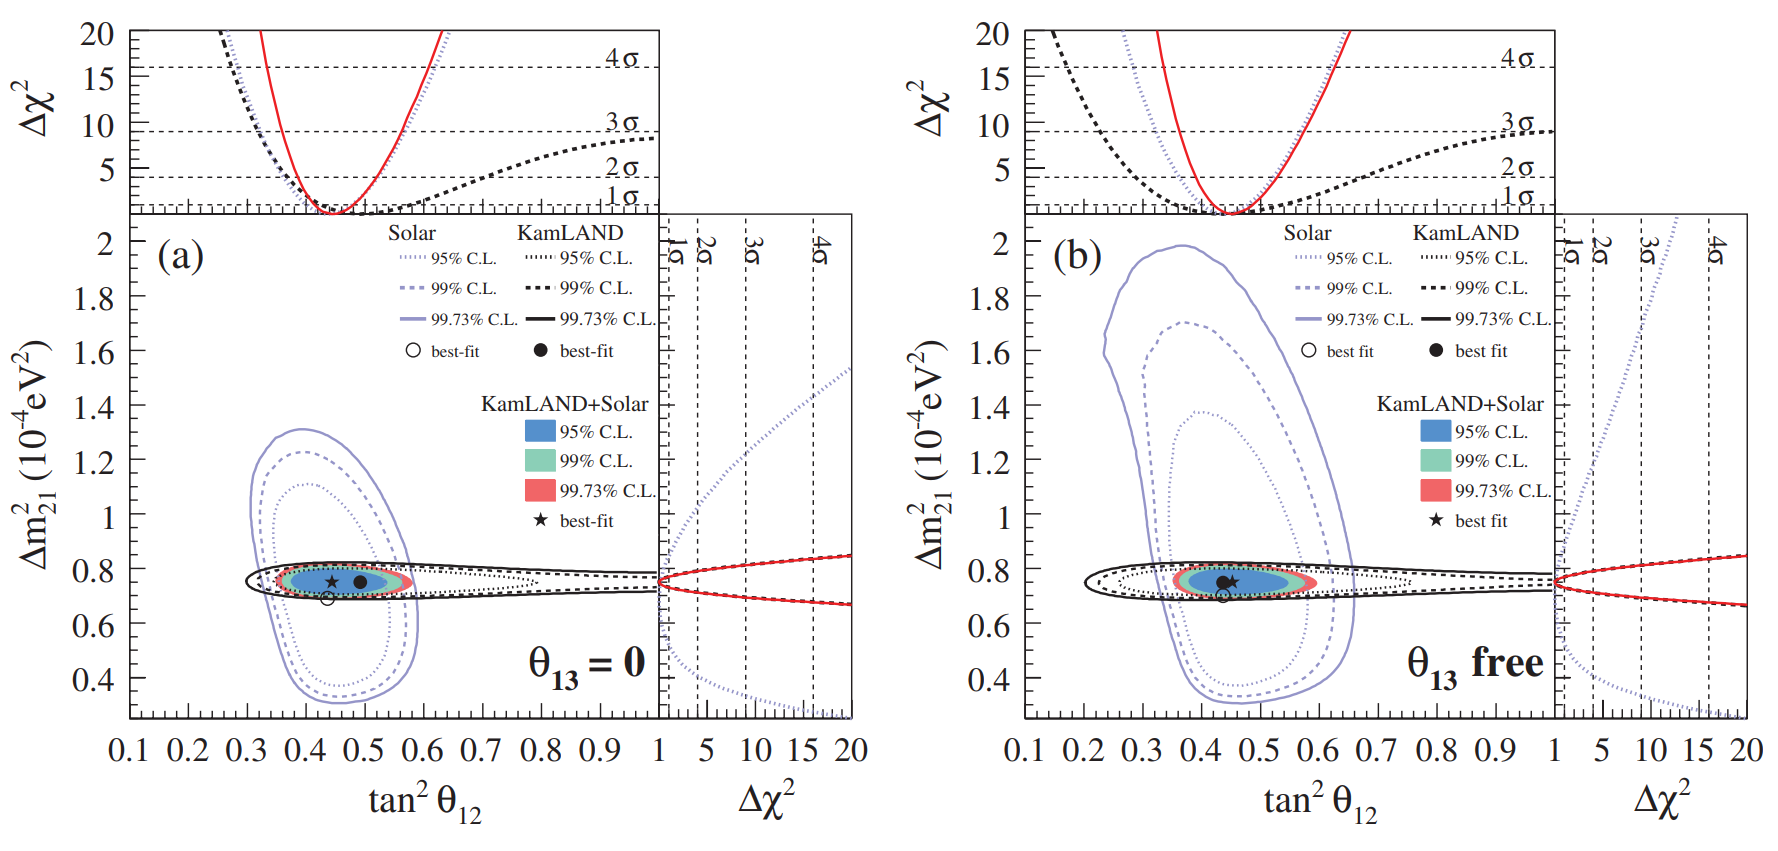
\includegraphics[width=0.7\textwidth, trim={0mm 0mm 0mm 0mm}, clip,page=1]{figures/theory/kamland_solar_comb}
	\caption{$\Delta m^2_{21}$ and $\theta_{21}$ measurements from KamLAND, SNO and SK (Solar). Figure from \cite{kamland_2011}.}
	\label{fig:21_sector}
\end{figure}

The short baseline reactor experiments at $\sim1\text{ km}$ have consistently measured neutrino event excess at $E_\nu\sim5\text{ MeV}$\cite{double_chooz, daya_bay, reno}, which is currently unresolved. The culprit is claimed to be either poor neutrino flux modelling or a sterile neutrino\cite{huber_neos,steriles}. As a result, very short baseline ($L\sim10-20\text{ m}$) experiments NEOS\cite{neos}, DANSS\cite{danss}, PROSPECT\cite{prospect}, STEREO\cite{stereo} and SoLi$\delta$\cite{solid} have been commissioned to measure $\bar{\nu}_e$ disappearance. None have found evidence of a sterile neutrino, and all have confirmed the 5 MeV excess.

  \chapter{The NEUT neutrino interaction event generator}
\label{chap:NEUT}

\section{Generator background}
\label{sec:NEUT:background}


  \chapter{The NUISANCE framework}
\label{chap:NUISANCE}

\section{Justification}
\label{chap:NUISANCE:justification}
large data-mc comparisons
compare different generators

\section{Framework structure}
\label{chap:NUISANCE:framework}

\section{Examples}
\label{chap:NUISANCE:examples}
  \chapter{Fitting NEUT single pion production}
\label{chap:1pi_fits}

\section{Background}
\label{sec:1pi_fits:background}


\section{Selecting data}
\label{sec:1pi_fits:data}


\section{Fitting}
\label{sec:1pi_fits:fit}


\section{Propagating results}
\label{sec:1pi_fits:prop}


  \chapter{Updating the single pion model}
\label{chap:1pi_update}

\section{Updating Rein-Sehgal ejection mechanism}
\label{sec:1pi_update:RS_ej}
\subsection{Theory}
\subsection{Implementation}
\subsection{Validation}
\subsection{Examples and results}
Compare to data, compare to other MC

\section{Implementing Monireh Kabirhnezhad single pion production}
\label{sec:1pi_update:Minoo}
\subsection{Theory}
\subsection{Implementation}
\subsection{Validation}
\subsection{Examples and results}
  
  \chapter{ND280 fits}
\label{chap:ND280}

\section{T2K}
The T2K experiment

\section{ND280}
Describe me

\section{Super-Kamiokande}

\section{T2K oscillation analysis chain overview}
\label{sec:oscchain}
The T2K oscillation analyses have a myriad of input groups providing central values and covariances for the systematic parameters. The ND280 beam group provides data on the neutrino beam, the NuMu and Nue systematics and selections groups provide ND280 systematics and suggested binning, the Neutrino Interactions Working Group (NIWG) provide neutrino interaction systematics, and the T2K-SK group provides systematics and selections for SK. Since ND280 and SK are in the same neutrino beam, the high-statistics neutrino samples at ND280 can be used to constrain the simulation prior to seeing data at SK. At the near-detector the flux model, neutrino interaction model and ND280 model is fit. Details on these systematics will be provided in \autoref{sec:syst}.

T2K has two separate groups fitting near-detector data with the intent of maximising model likelihood: BANFF (Beam And Near detector Flux task Force) and MaCh3 (Markov Chain 3 flavour oscillation fitter). The two frameworks use identical event selections and systematic parameters, outlined in \autoref{sec:ND280:sel} and \autoref{subsec:syst_nd280}, but entirely different methods of evaluating the model goodness and exploring the parameter space.

BANFF interfaces to the popular gradient-descent minimizer MINUIT \red{CITE} and MaCh3 uses a custom Markov Chain Monte Carlo sampler to sample the high dimensional parameter space\red{cite metropolis hastings?}. Importantly, the BANFF attempts to find the global minimum of the test-statistic given the data and the model, whereas MaCh3 explores an area around the minimum test-statistic with the intent of sampling the Bayesian posterior. Therefore, MaCh3 does not necessarily locate a set of ``best-fit'' parameters with covariances assuming a parabolic minimum: instead it provides a full high-dimensional posterior with arbitrary shape. Once the model is constrained by near-detector data, the T2K oscillation analysis chain can then proceed using the model proposed by the near-detector data and model and include oscillation effects.

However, providing a high-dimensional posterior of arbitrary shape is cumbersome, so oscillation groups often use the BANFF output. MaCh3 has the advantage of a near and far detector implementation, meaning a simultaneous fit of data from both detectors can be done. This avoids assumptions on the underlying probability distribution functions of the parameters and the likelihood surface, and additionally benefits from fully correlating the models at both detectors, allowing one to affect the other as the fit proceeds.

The following sections detail the near-detector implementation of the MaCh3 framework. It also includes comparisons and validations to the BANFF framework. It finishes with the 2017 round fit to data.

\section{Need for ND280 fits}
As statistics increase at Super-Kamiokande, there is more and more need for well-controlled systematics. The T2K oscillation analysis uses \red{CITEME}

SK without constraints
Share same beam, use near detector complex
  \section{Selections}
\label{sec:ND280:sel}
The goal of the selection is to map interaction modes (e.g. CCQE, CC1$\pi^+$, CC DIS) to observable ND280 selections, so that theory parameters receive their largest constraints from a few exclusive selections. Equivalent FGD1 and FGD2 selections are separated due to differences in systematics and reconstruction: forward-going tracks emanating in FGD1 leaves a track in FGD1, TPC2, FGD2 and TPC3, so has more hits recorded than the FGD2 equivalence, which only passes through FGD2 and TPC3. Furthermore, FGD2 contains plastic scintillator interleaved with passive water layers whereas FGD1 is fully plastic scintillator. Separating FGD1 and FGD2 also allows constraints on water interactions to come strictly from the FGD2 selections.

The events in the analysis are binned in reconstructed muon candidate variables \pmu and \cosmu. The muon variables are chosen primarily due to excellent detector resolution of muons and for consistency with analyses at SK. There is ongoing effort to include pion variables when such are present (e.g. for CC$1\pi^+$ or CCOther selections), and composite variables in the plane transverse to the neutrino, but will not be presented here.

The selections are entirely defined by the observed reconstructed event topology of an event in the detector and there is no attempt at correcting for misidentified particles. There is no attempt to correct for nuclear effects such as final-state-interactions (FSI).

\subsection{\numu in FHC}
\label{sec:numu_sel}
The different topological selections start by isolating CC-inclusive candidates in FGD1 and FGD2. First, an event is required to contain one reconstructed track of negative charge crossing the TPC downstream of either FGD. The event also needs to fulfil data quality and fiducial volume requirements. The muon is assumed to be the highest momentum negative track (HMNT) found in the event, and it is required that the track is identified as a muon.

The detailed selection criteria for the CC-inclusive sample is:
\begin{itemize}
	\item \textbf{Event quality cut}: The full beam spill has a good global ND280 data quality flag, meaning all ND280 sub-detectors and magnet were operational and reading out data. The event must occur within the bunch time window of the neutrino beam. Event pile-up is mitigated by associating each event to a beam bunch within a beam spill.
	
	\item \textbf{Quality and fiducial volume cut}: At least one reconstructed track is present in the FGD1 or FGD2 fiducial volumes. The fiducial volume for FGD1 is $|x|<874.51\text{ mm}$, $|y-55|<874.51\text{ mm}$, $136.875 < z < 446.955\text{ mm}$ and for FGD2 $|x|<874.51\text{ mm}$, $|y-55|<874.51\text{ mm}$, $1481.45< z < 1807.05\text{ mm}$\footnote{The 55mm offset in $y$ reflects the shift in XY modules relative the center of the ND280 coordinate system.}.
	
	The $x$ and $y$ cuts are designed to accept interactions which have their vertex five bars from the edge of the XY module of each FGD. The $z$ cut excludes the first XY module of each FGD and includes the remaining (14 for FGD1, seven for FGD2). To reject short tracks, for which the TPC reconstruction is unreliable, tracks are required to have more than 18 TPC clusters.
	
	\item \textbf{Upstream background veto}: If the second highest momentum track starts at least 150 mm upstream of the selected muon candidate the event is rejected. This cut eliminates events in which the muon candidate might be the second part of a broken track which started further upstream. For events with a reconstructed vertex in FGD2 there is the added criterion of having no reconstructed tracks in FGD1.
	
	\item \textbf{Broken track cut}: The starting position of the muon candidate track needs to be less than 425 mm away from the FGD upstream edge if the event has at least one reconstructed FGD-only track. The cut vetoes events where the reconstruction has cut a muon candidate track into two tracks: one of which is fully contained in the FGD and the other which starts downstream of the fully contained, misplacing the interaction vertex.
	
	\item \textbf{Muon PID cut}: Once a particle is considered a muon candidate, the particle identification is applied based on the observed $dE/dx$ measurement of the track in the TPC. The measured energy deposit $E$ in the TPC is compared with the expected energy deposit under muon, pion, electron and proton hypotheses and pulls and discrimination functions are applied.
	
	The pulls $\delta_i$ for particle type $i$ are defined as
	\begin{equation}
	\label{eq:tpc_track_chi2}
	\delta_i = \frac{C_T^{obs}-C_T^{exp}}{\sigma^{exp}}
	\end{equation}
	where the expected energy loss $C_T^{exp}$ is parameterised as
	\begin{equation}
	C_T^{exp} = \frac{53.87 \text{ ADC}}{\beta^{2.283}} \left( 5.551 - \beta^{2.283} - \log\left[0.001913 + \frac{1}{\left(\beta\gamma\right)^{1.249}}\right]\right)
	\end{equation}
	$C_T^{obs}$ is the observed energy loss and $\sigma^{exp}$ is the deposited energy resolution of the TPC. ADC refers to the analog to digital counts read out from the detector, indicative of the energy deposited by the particle. $\beta=v/c$ and $\gamma = 1/\sqrt{1-\beta^2}$ are the relativistic variables of the track. The TPC pulls after preselection are shown in \autoref{fig:numu_pulls}
	
	The likelihoods $\mathcal{L}_i$ are then defined as
	\begin{equation}
	\label{eq:tpc_track_likelihood}
		\mathcal{L}_i = \frac{e^{-\delta^2_i}}{\sum_n e^{-\delta^2_n}}
	\end{equation}
	where the denominator is summed over the particle types $n=\mu,\pi,e,p$. The likelihoods are shown in \autoref{fig:numu_likelihoods}. In the PID algorithm, electrons are rejected by requiring a MIP likelihood
	\begin{equation}
		\label{eq:tpc_track_mip}
		\mathcal{L}_{MIP} = \frac{\mathcal{L}_\mu + \mathcal{L}_\pi}{1-\mathcal{L}_p} > 0.8
	\end{equation}
	for tracks with $p<500\text{ MeV/c}$. To remove protons and pions, it is also required that
	\begin{equation}
	\label{eq:tpc_track_mu}
		\mathcal{L}_\mu > 0.05
	\end{equation}
	The constants 0.8, 0.05 and 500 MeV/c are chosen from particle gun studies in the TPC and test-beam data\cite{t2k_tpc,thesis_tpc, thesis_christine}. The energy loss in the TPC from which the pulls are derived are shown in \autoref{fig:TPC_dedx}. Importantly, TPC segments need to pass the TPC track quality cut to contribute to the likelihood: bad quality tracks do not. If a track passes through multiple TPCs all TPC tracks are taken into account.
\end{itemize}

\begin{figure}[h]
	\begin{subfigure}[t]{0.49\textwidth}
		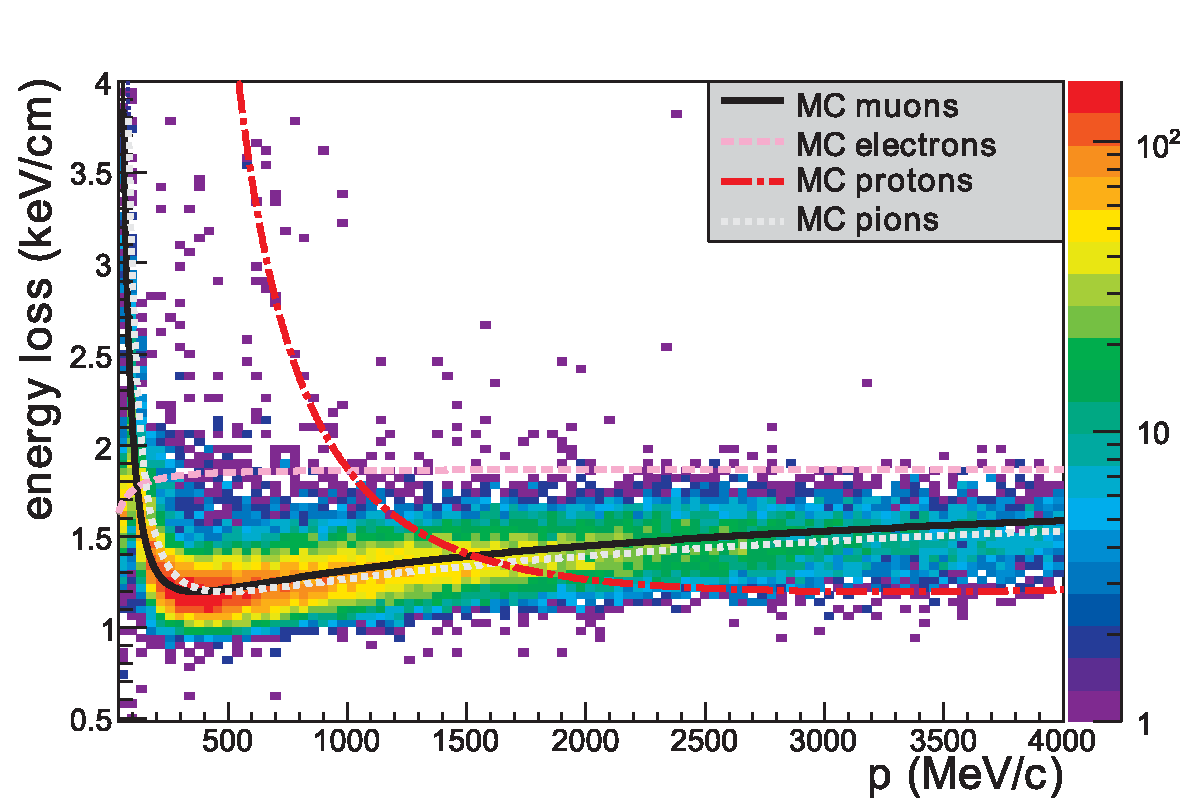
\includegraphics[width=\textwidth]{figures/numu/TPC_PID_neg}
		\caption{Negative particles}
	\end{subfigure}
	\begin{subfigure}[t]{0.49\textwidth}
		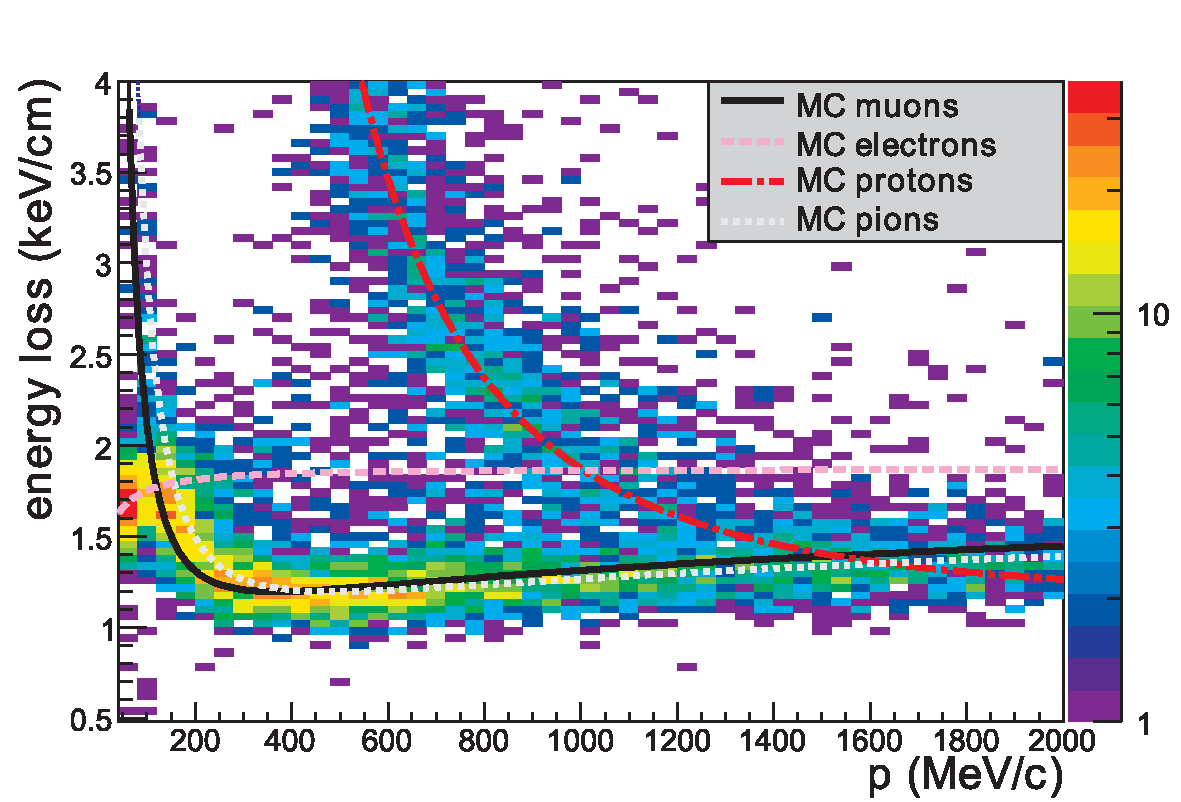
\includegraphics[width=\textwidth]{figures/numu/TPC_PID_pos}
		\caption{Positive particles}
	\end{subfigure}
	\caption{The energy loss for particles travelling through the TPC}
	\label{fig:TPC_dedx}
\end{figure}

\begin{figure}[h]
	\begin{subfigure}[t]{0.49\textwidth}	
		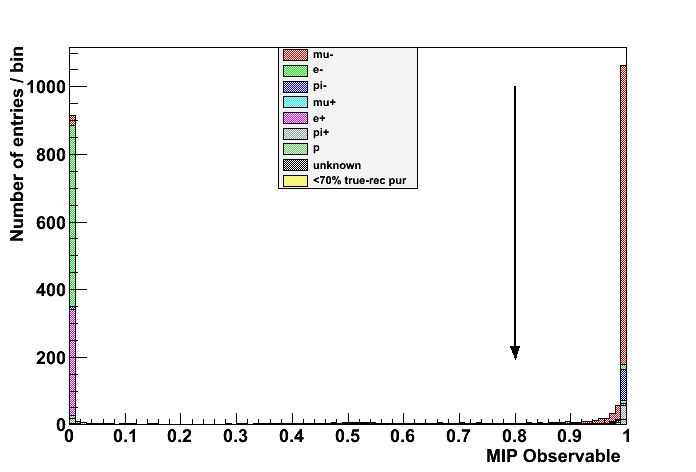
\includegraphics[width=\textwidth]{figures/numu/Cuts/numu/Miplik_run12}
		\caption{$\mathcal{L}_{MIP}$}
	\end{subfigure}
	\begin{subfigure}[t]{0.49\textwidth}	
		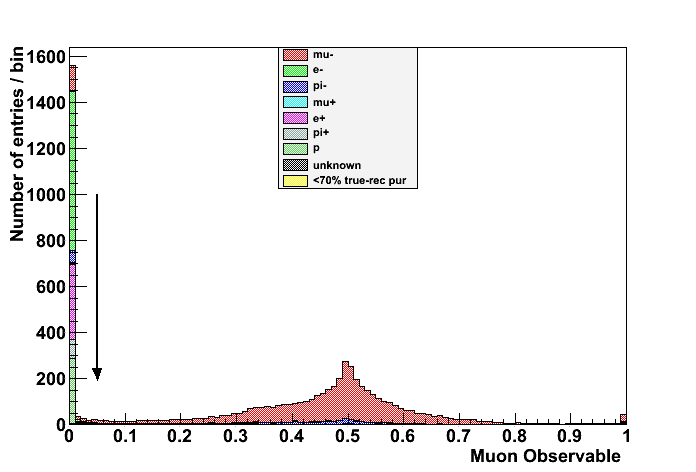
\includegraphics[width=\textwidth]{figures/numu/Cuts/numu/Mulik_run12}
		\caption{$\mathcal{L}_{\mu}$}
	\end{subfigure}
	\caption{Likelihood distributions for preselected MC events, showing cuts placed for \numu in FHC analysis}
	\label{fig:numu_likelihoods}
\end{figure}

\begin{figure}[h]
	\begin{subfigure}[t]{0.32\textwidth}
		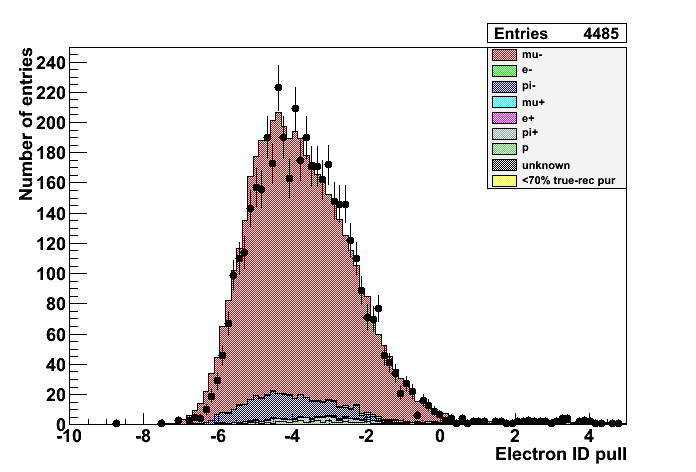
\includegraphics[width=\textwidth]{figures/numu/Cuts/numu/Elepull_run12}
		\caption{$\delta_e$---the electron ID pull}
	\end{subfigure}
	\begin{subfigure}[t]{0.32\textwidth}	
		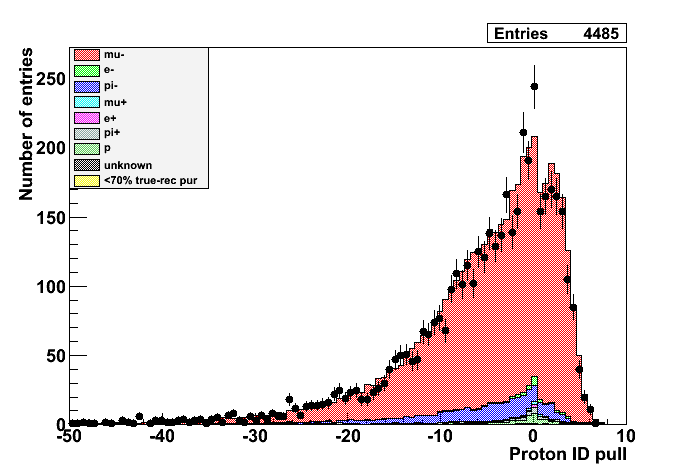
\includegraphics[width=\textwidth]{figures/numu/Cuts/numu/Protpull_run12}
		\caption{$\delta_p$---the proton ID pull}
	\end{subfigure}
	\begin{subfigure}[t]{0.32\textwidth}
		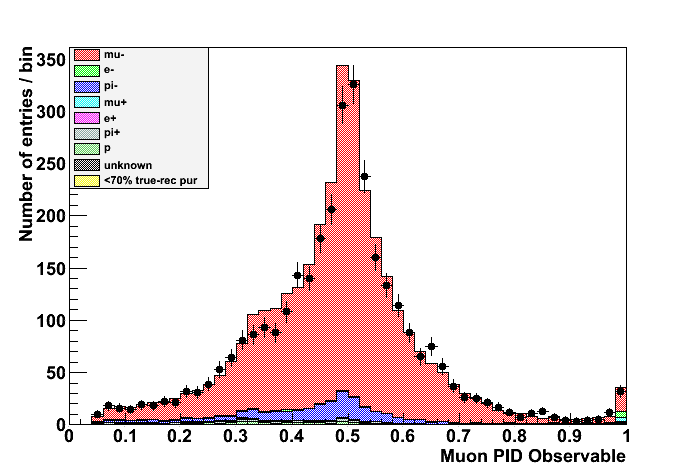
\includegraphics[width=\textwidth]{figures/numu/Cuts/numu/Mulikelihood_run2}
		\caption{$\delta_\mu$---the muon ID pull}
	\end{subfigure}
	\caption{Pull distributions for particle hypotheses after selection showing data and MC for \numu analysis}
	\label{fig:numu_pulls}
\end{figure}

The selection criteria proceeds to split the CC-inclusive sample into the three subsamples: CC$0\pi$, CC$1\pi$ and CCOther. This is based entirely on pion identification in the TPCs and FGDs. To identify pion candidate(s) a number of cuts are applied:
\begin{itemize}
	\item \textbf{Muon candidate}: The track can not be identified as the above muon candidate.
	
	\item \textbf{Matching beam spill and bunch}: The pion candidate is required to originate from the same beam bunch and spill to the identified muon candidate.
	
	\item \textbf{Track origin}: The pion candidate is required to start in the same FGD fiducial volume as the muon candidate and enter the downstream TPC for PID purposes. The same FGD and TPC track quality and fiducial volume cut is applied for the pion candidate as for the muon candidate.
	
	\item \textbf{Pion PID}: For positive tracks in the TPC, pion, positron and proton hypotheses are tested. For negative tracks, pion and electron hypotheses are tested. 
	
	As for the muon candidate, \autoref{eq:tpc_track_chi2} and \autoref{eq:tpc_track_likelihood} define the particle likelihoods. For the pion PID, the MIP likelihood in \autoref{eq:tpc_track_mip} is required and in addition a cut on the pion likelihood is invoked,
	\begin{equation}
	\label{tpc_track_pi}
		\mathcal{L}_\pi > 0.3
	\end{equation}
	
	When there is no particle track in the TPC, the FGD PID is used to count the number of charged pions. However, it can not be used for neutral pions because there is currently no electron or positron reconstruction available in the FGD. The FGD pion PID proceeds either by:
	\begin{itemize}
		\item \textbf{Michel electron tag}: A search for a Michel electron tag is made for low-momentum tracks that fail to leave enough hits for track reconstruction. It looks for a time-delayed FGD hit cluster out of time with a beam bunch window. A Michel candidate is found if the number of hits in the delayed time bin is greater than six for FGD1 and five for FGD2\footnote{Roughly corresponding to 200 photoelectrons, which can't be used as a criteria in FGD2 due to the water layers}. Since there is no measurement of the track, the pion has no associated momentum or angle.
		
		\item \textbf{FGD reconstruction}: Higher momentum pions may leave fully contained tracks in the FGD. If such a track belongs to the same bunch as the muon candidate and there is only one pion track reconstructed in the FGD, it is considered a pion candidate. The pion candidate is required to be upwards or downwards-going by invoking $|\cos\theta_{\pi,\nu}| > 0.3$, which limits the possibility of travelling along the FGD bars. Finally we require a pion pull of $-2 < P_\pi < 2.5$ in the FGD from its track length, shown in \autoref{fig:FGD_pion_pulls}.
	\end{itemize}
\end{itemize}
\begin{figure}[h]
	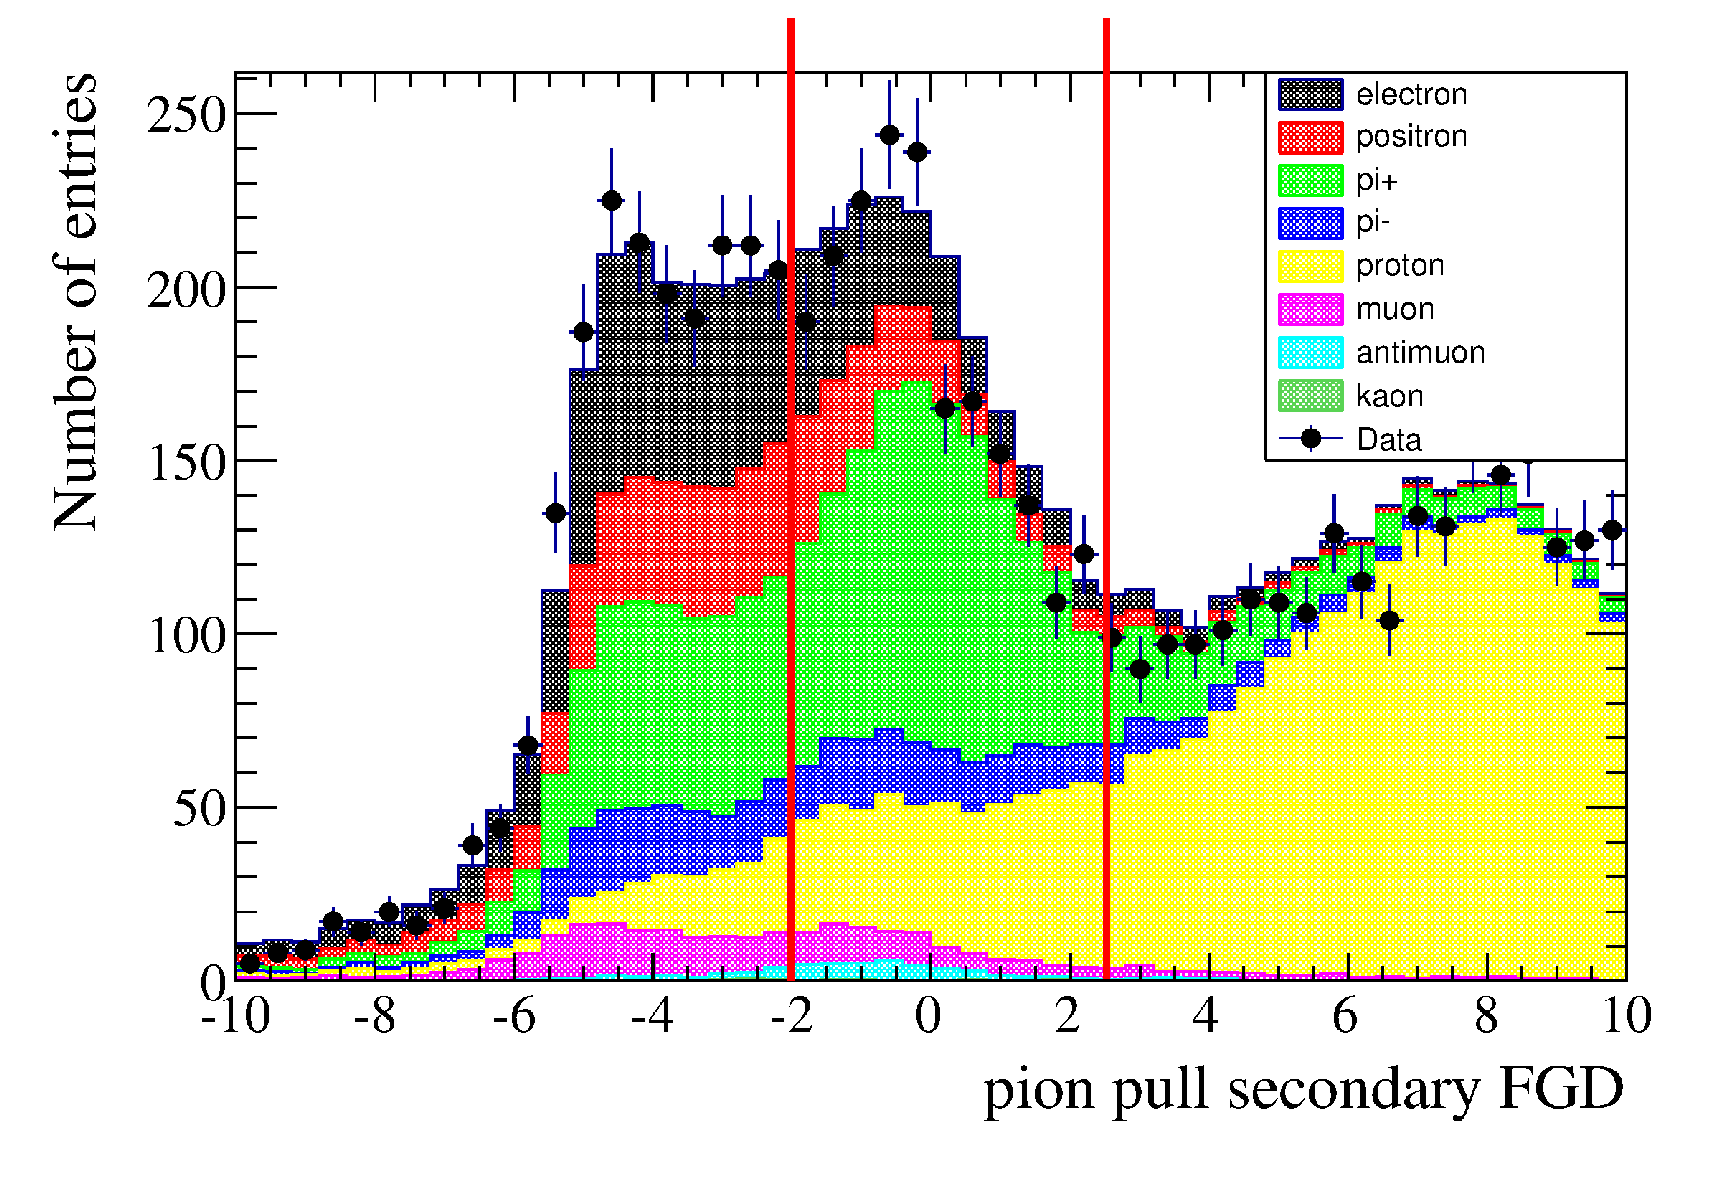
\includegraphics[width=0.5\textwidth]{figures/numu/Cuts/pull_secondarytrack_FGD_all.eps}
	\caption{FGD1 pion pulls for a fully contained track}
	\label{fig:FGD_pion_pulls}
\end{figure}

Finally, the remaining particles can be identified using the TPC PID: 
\begin{itemize}
	\item For a positive particle, it is tagged according to highest probability. If the most likely particle is a positron but the $p_{reco} > 900\text{ MeV}$ it's tagged as a proton, otherwise it is a positron.
	
	\item For a negative particle, if the probability of a pion is $P_\pi>0.8$ it is tagged as a negative pion, and if not it is assumed an electron.
\end{itemize}

Using information from the TPC PID, FGD Michel electron and FGD PID algorithms, the \numu CC-inclusive sample is categorised into the CC$0\pi$, CC$1\pi$ and CCOther samples:
\begin{itemize}
	\item \textbf{CC0$\pi$}: Contains events with one negative muon candidate, no identified charged or neutral pions in the TPC or FGD, and no electrons or positrons in the TPC. The selection predominantly contains CCQE and 2p2h events and is the largest sample at ND280. An example event display is shown in \autoref{fig:cc0pi_evtdisplay}.
	\begin{figure}[h]
		\begin{subfigure}[t]{0.49\textwidth}
			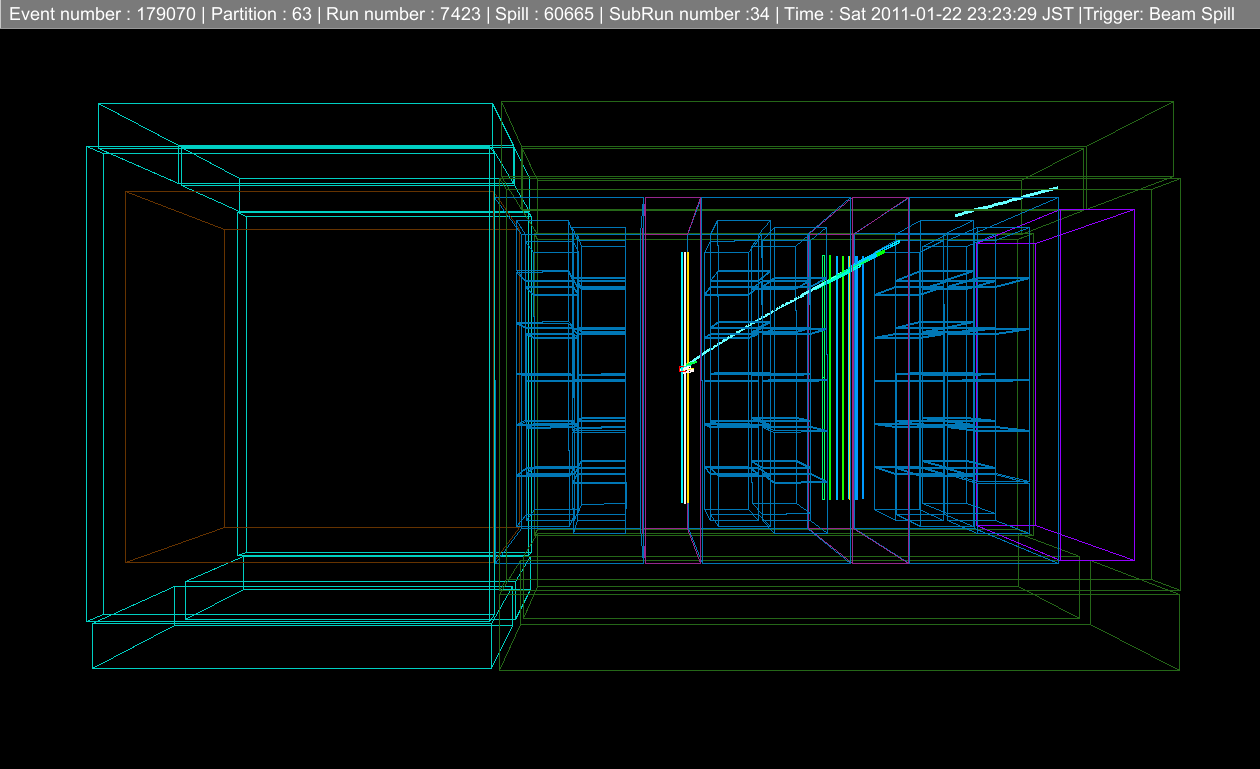
\includegraphics[width=\textwidth, trim={25mm 28mm 30mm 30mm}, clip]{figures/numu/evtdisplay/CC0pi_7423_34_179070_perX0Z_all}
			\caption{Side-view}
		\end{subfigure}
		\begin{subfigure}[t]{0.49\textwidth}
			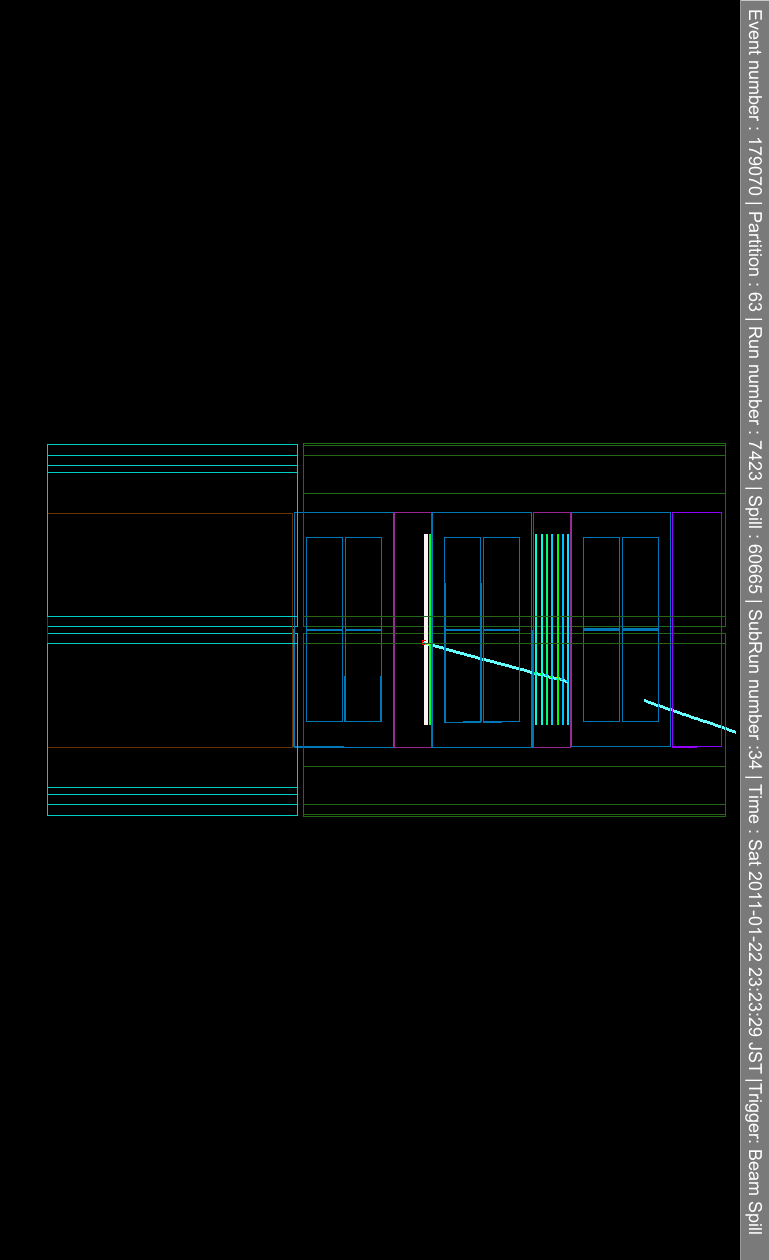
\includegraphics[width=\textwidth, trim={10mm 150mm 10mm 150mm}, clip]{figures/numu/evtdisplay/CC0pi_7423_34_179070_ortX0Z_all}
			\caption{Top-view}
		\end{subfigure}
		\caption{True FGD1 CC0$\pi$ event display in ND280}
		\label{fig:cc0pi_evtdisplay}
	\end{figure}

	\item \textbf{CC$1\pi$}: Contains events with one negative muon candidate and one positive pion candidate. The sum of the number of positive pions found in the TPC and the number of Michel electrons is one and if there are no Michel electrons the sum of positive pions in the TPC and fully contained in the FGD is one. If there is a negative pion, electron or positron reconstructed in the TPC it is rejected. The selection contains mostly CC1$\pi^{+}$ and multi-$\pi^+$ events from resonant and DIS interactions. An example event display is shown in \autoref{fig:cc1pi_evtdisplay}.
	\begin{figure}[h]
		\begin{subfigure}[t]{0.49\textwidth}
			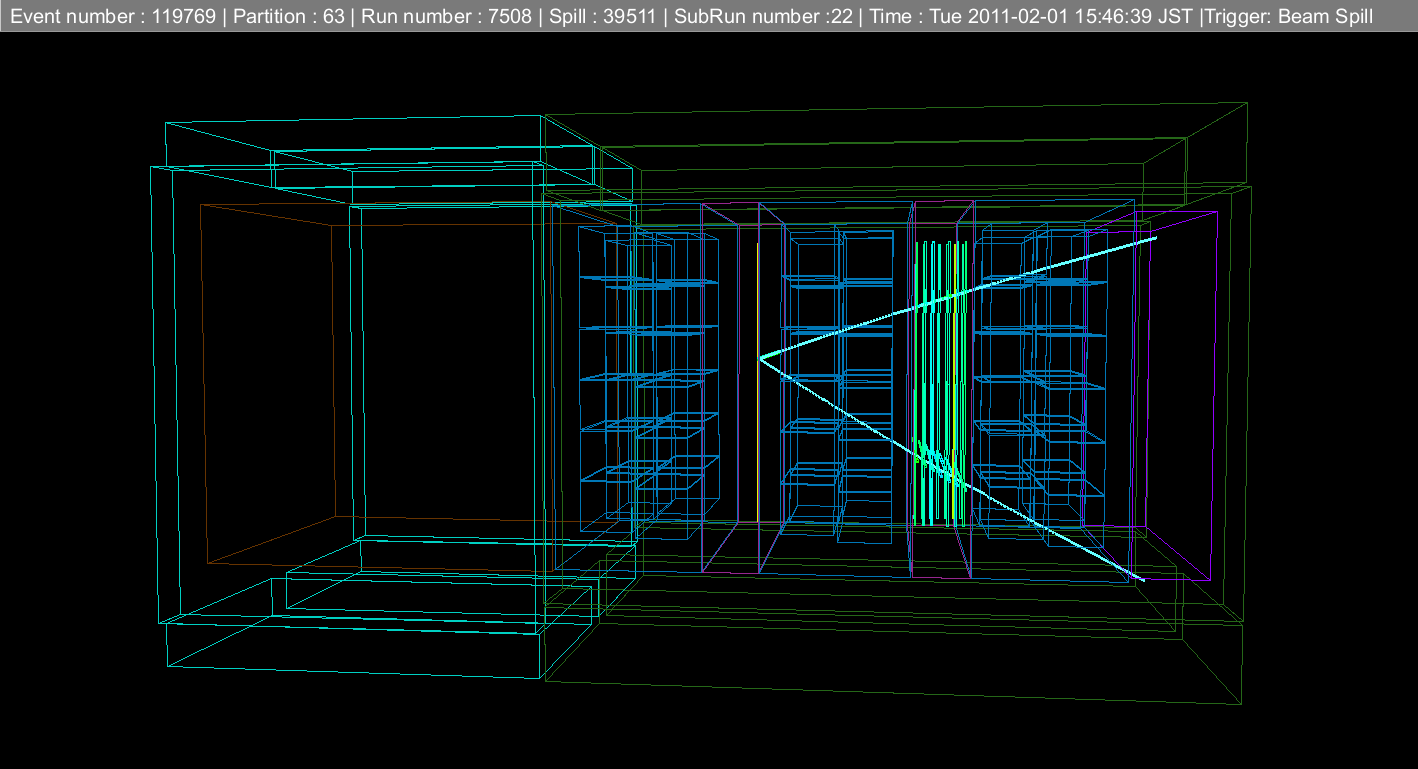
\includegraphics[width=\textwidth, trim={50mm 30mm 50mm 40mm}, clip]{figures/numu/evtdisplay/CC1pi_7508_22_119769_perpX0Z_all}
			\caption{Side-view}
		\end{subfigure}
		\begin{subfigure}[t]{0.49\textwidth}
			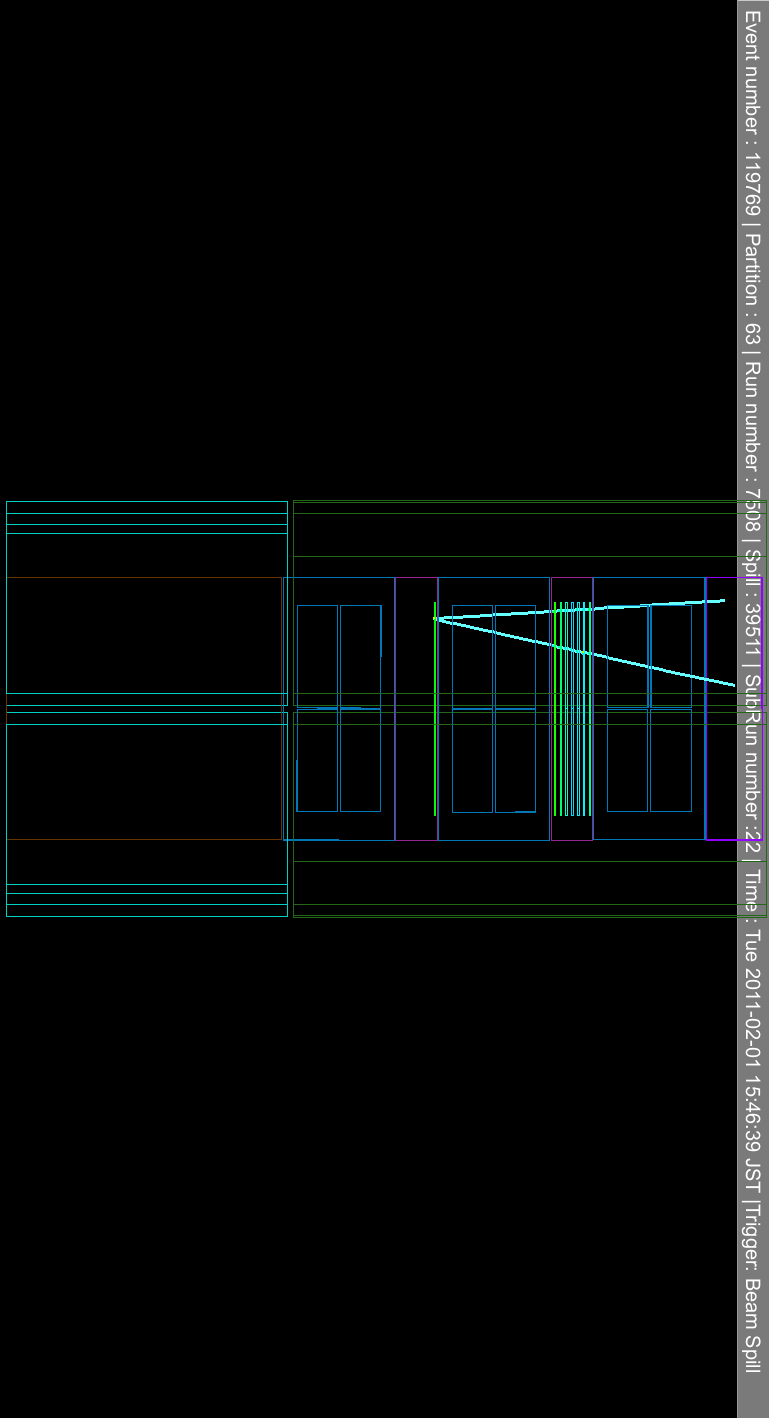
\includegraphics[width=\textwidth, trim={0mm 170mm 10mm 170mm}, clip]{figures/numu/evtdisplay/CC1pi_7508_22_119769_ortX0Z_all}
			\caption{Top-view}
		\end{subfigure}
		\caption{True FGD1 CC1$\pi$ event display in ND280}
		\label{fig:cc1pi_evtdisplay}
	\end{figure}
	
	\item \textbf{CCOther}: All events with one negative muon candidate which are not classified as CC0$\pi$ or CC$1\pi$ fall into this sample. Events with one or more reconstructed negative pion(s), or one or more neutral pion(s) reconstructed as electron or positron candidates in the TPC, are thereby selected. Event with more than one positive pion based on the TPC and FGD pion counting criteria are also accepted. The selection contains mostly multi-$\pi$, DIS and CC$1\pi^0$ interactions. An example event display is shown in \autoref{fig:ccoth_evtdisplay}.
	\begin{figure}[h]
		\begin{subfigure}[t]{0.49\textwidth}
			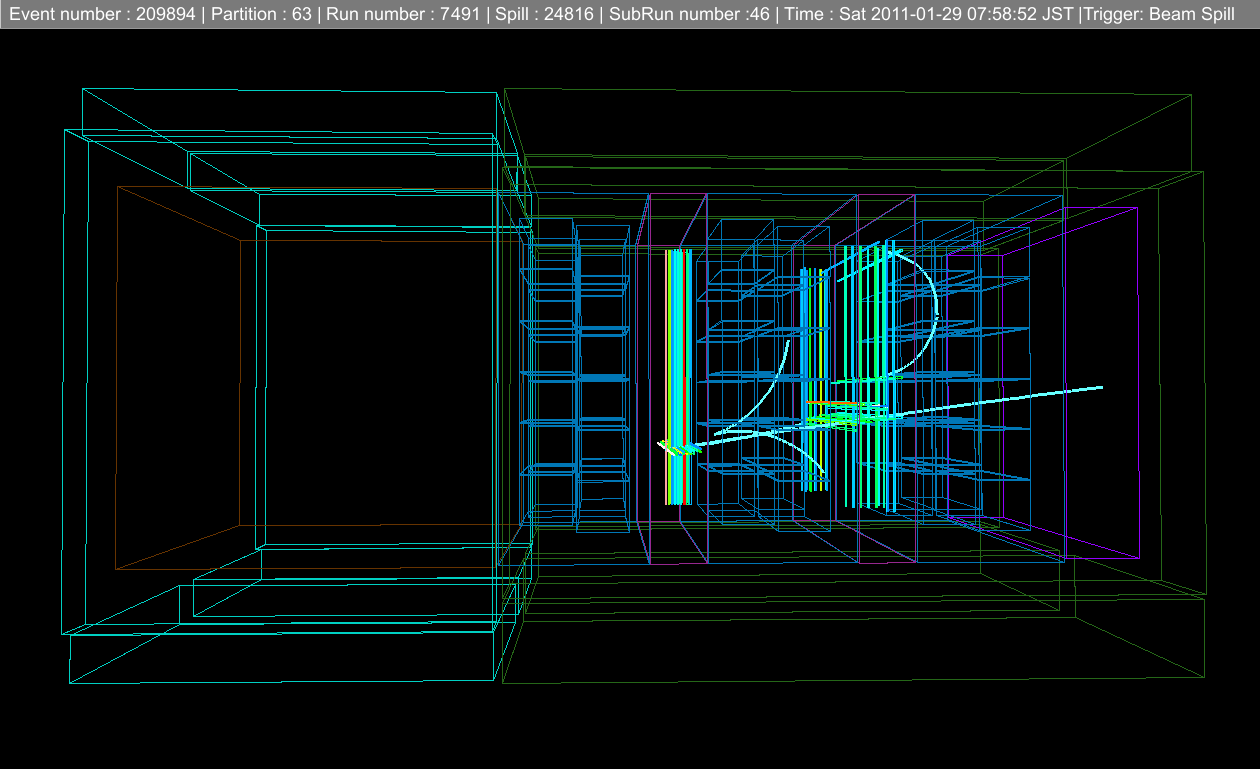
\includegraphics[width=\textwidth, trim={20mm 30mm 20mm 30mm}, clip ]{figures/numu/evtdisplay/CCOthers_7491_46_209894_perX0Z_all}
			\caption{Side-view}
		\end{subfigure}
		\begin{subfigure}[t]{0.49\textwidth}
			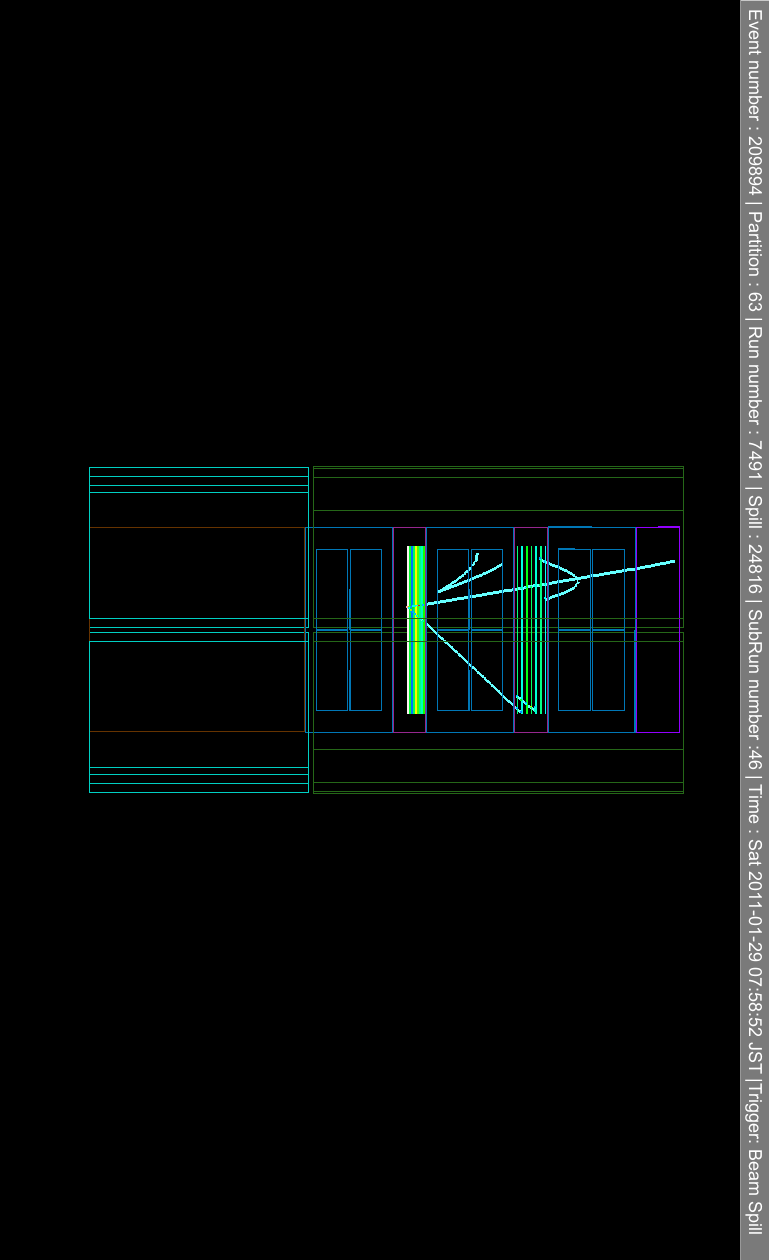
\includegraphics[width=\textwidth, trim={3cm 16cm 3cm 16cm}, clip]{figures/numu/evtdisplay/CCOthers_7491_46_209894_ortX0Z_all}
			\caption{Top-view}
		\end{subfigure}
		\caption{True FGD1 CCOther event display in ND280}
		\label{fig:ccoth_evtdisplay}
	\end{figure}
\end{itemize}

\subsection{\numubar in RHC}
\label{sec:numubar_sel}
The anti-neutrino CC1Track and CCNTrack selections have the same event quality and fiducial volume cut as the neutrino selection, and the muon candidate track is required to pass through the TPC downstream of the struck FGD. The highest momentum track is required to be the highest momentum positive track for its muon PID. The selections generally have a larger background of ``wrong-sign'' events: $\nu_x$ interactions producing $x^-$ which are identified as $\mu^+$, and $\nu_x$ interactions producing a $\pi^+$ which may be identified as the lepton candidate. Hence, the selection cuts proceed differently:
\begin{itemize}
	\item \textbf{Positive multiplicity}: The muon candidate track charge is required to be a highest momentum positive track, which removes a large amount of wrong-sign interactions
	
	\item \textbf{TPC veto}: Veto backwards-going events starting in the FGD and events coming from the P0D and the magnet by utilising the upstream TPCs. If the upstream TPC of an FGD has hits the event is rejected
	
	\item \textbf{Positive muon identification}: The TPC PID outlined for the \numu selections are used to select the positive muon candidate, with the cuts optimised for $\mu^+$. 
	
	$\mathcal{L}_{MIP}$ is defined identically to \autoref{eq:tpc_track_mip} although the cut is now placed at 0.9, and still applies only to particles with $p < 500\text{ MeV}$. The muon likelihood cut is modified to $0.1 < \mathcal{L}_\mu < 0.7$ which removes protons and positive pions from the \numu background. The upper bound at 0.7 is present to reject low energy wrong-sign muons, which may be misidentified as positive tracks. The likelihood distributions and impact of these cuts are shown in \autoref{fig:numubar_likelihood} and \autoref{fig:numubar_likelihood_sel} for the selected lepton candidate. \autoref{fig:numubar_pulls} shows the TPC PID pulls for run5+6.
\end{itemize}

\begin{figure}[h]
	\begin{subfigure}[t]{0.49\textwidth}
		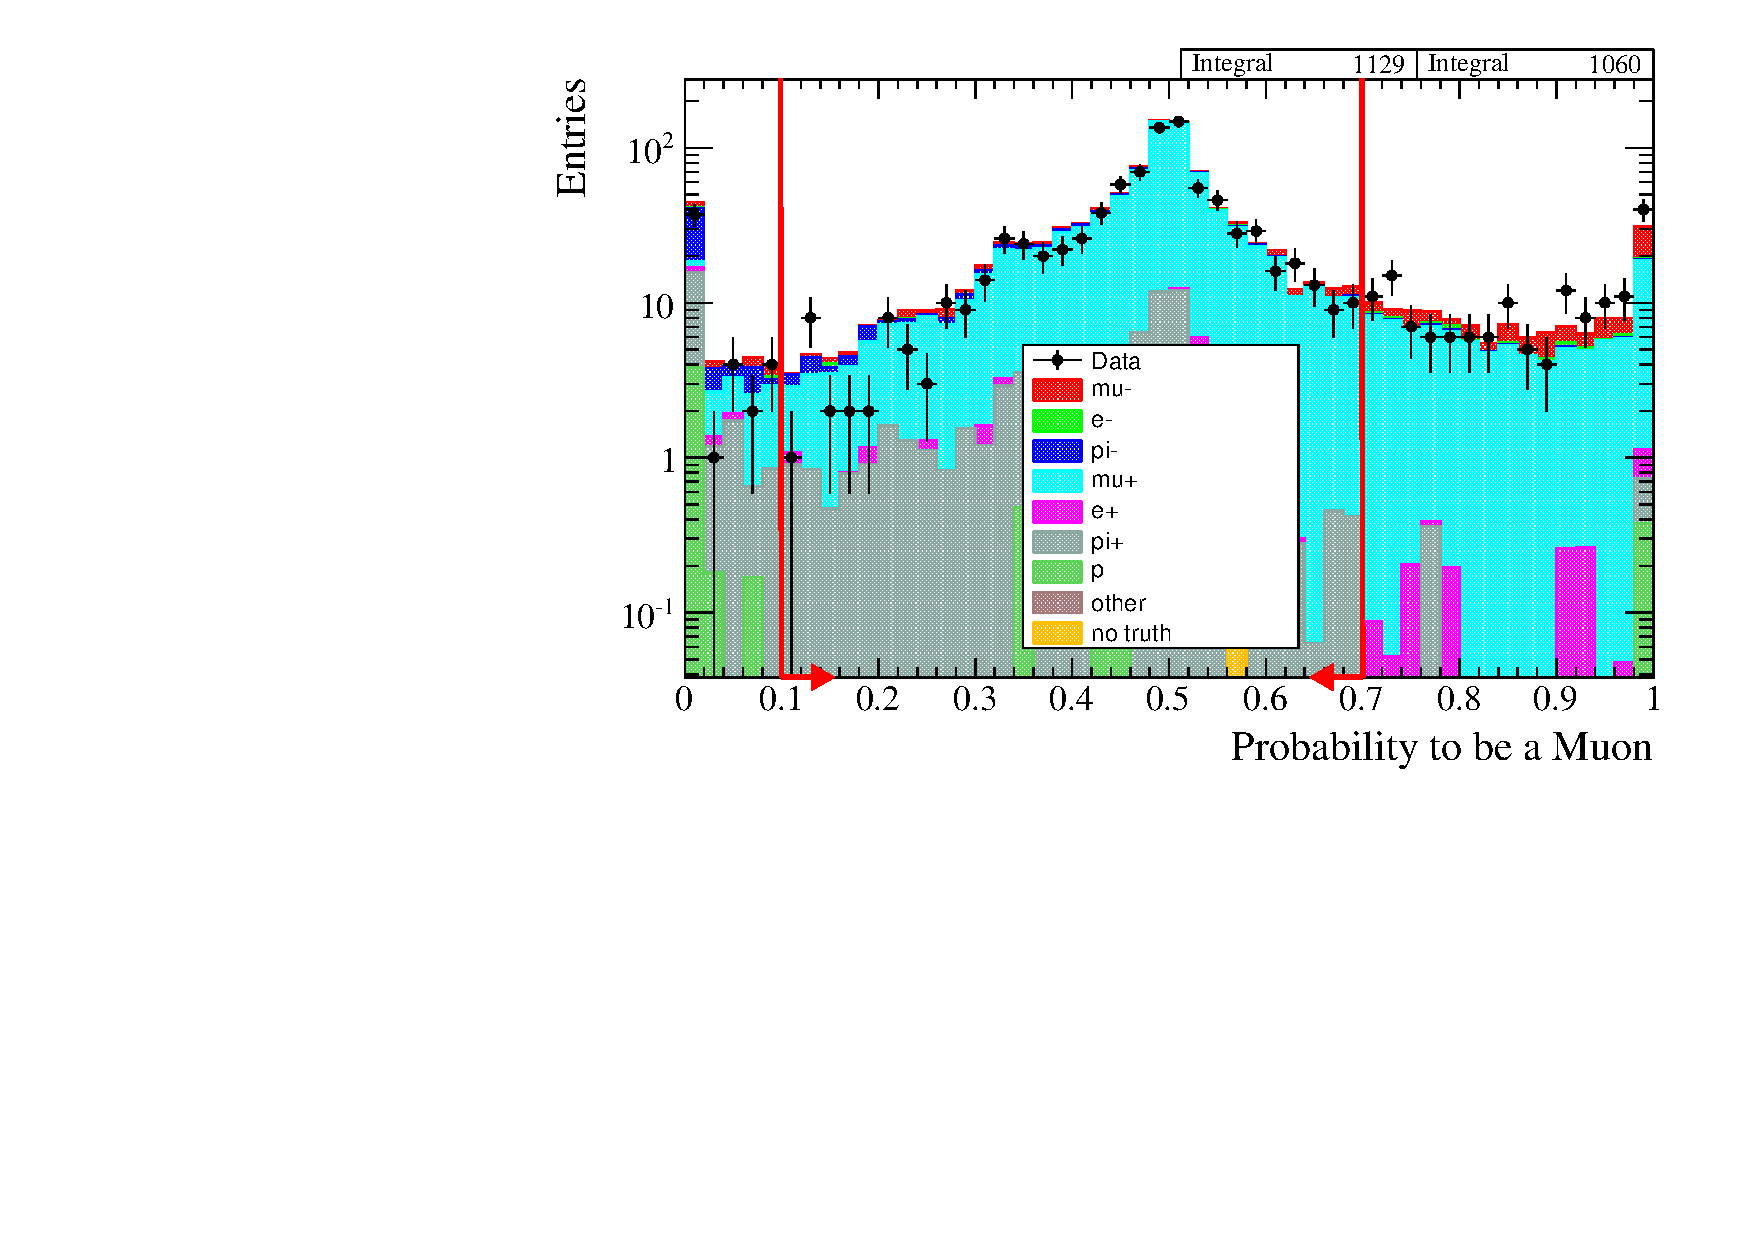
\includegraphics[width=\textwidth]{figures/numu/Cuts/numubar/likemu_numubar}
		\caption{$\mathcal{L}_\mu$}
	\end{subfigure}
	\begin{subfigure}[t]{0.49\textwidth}
		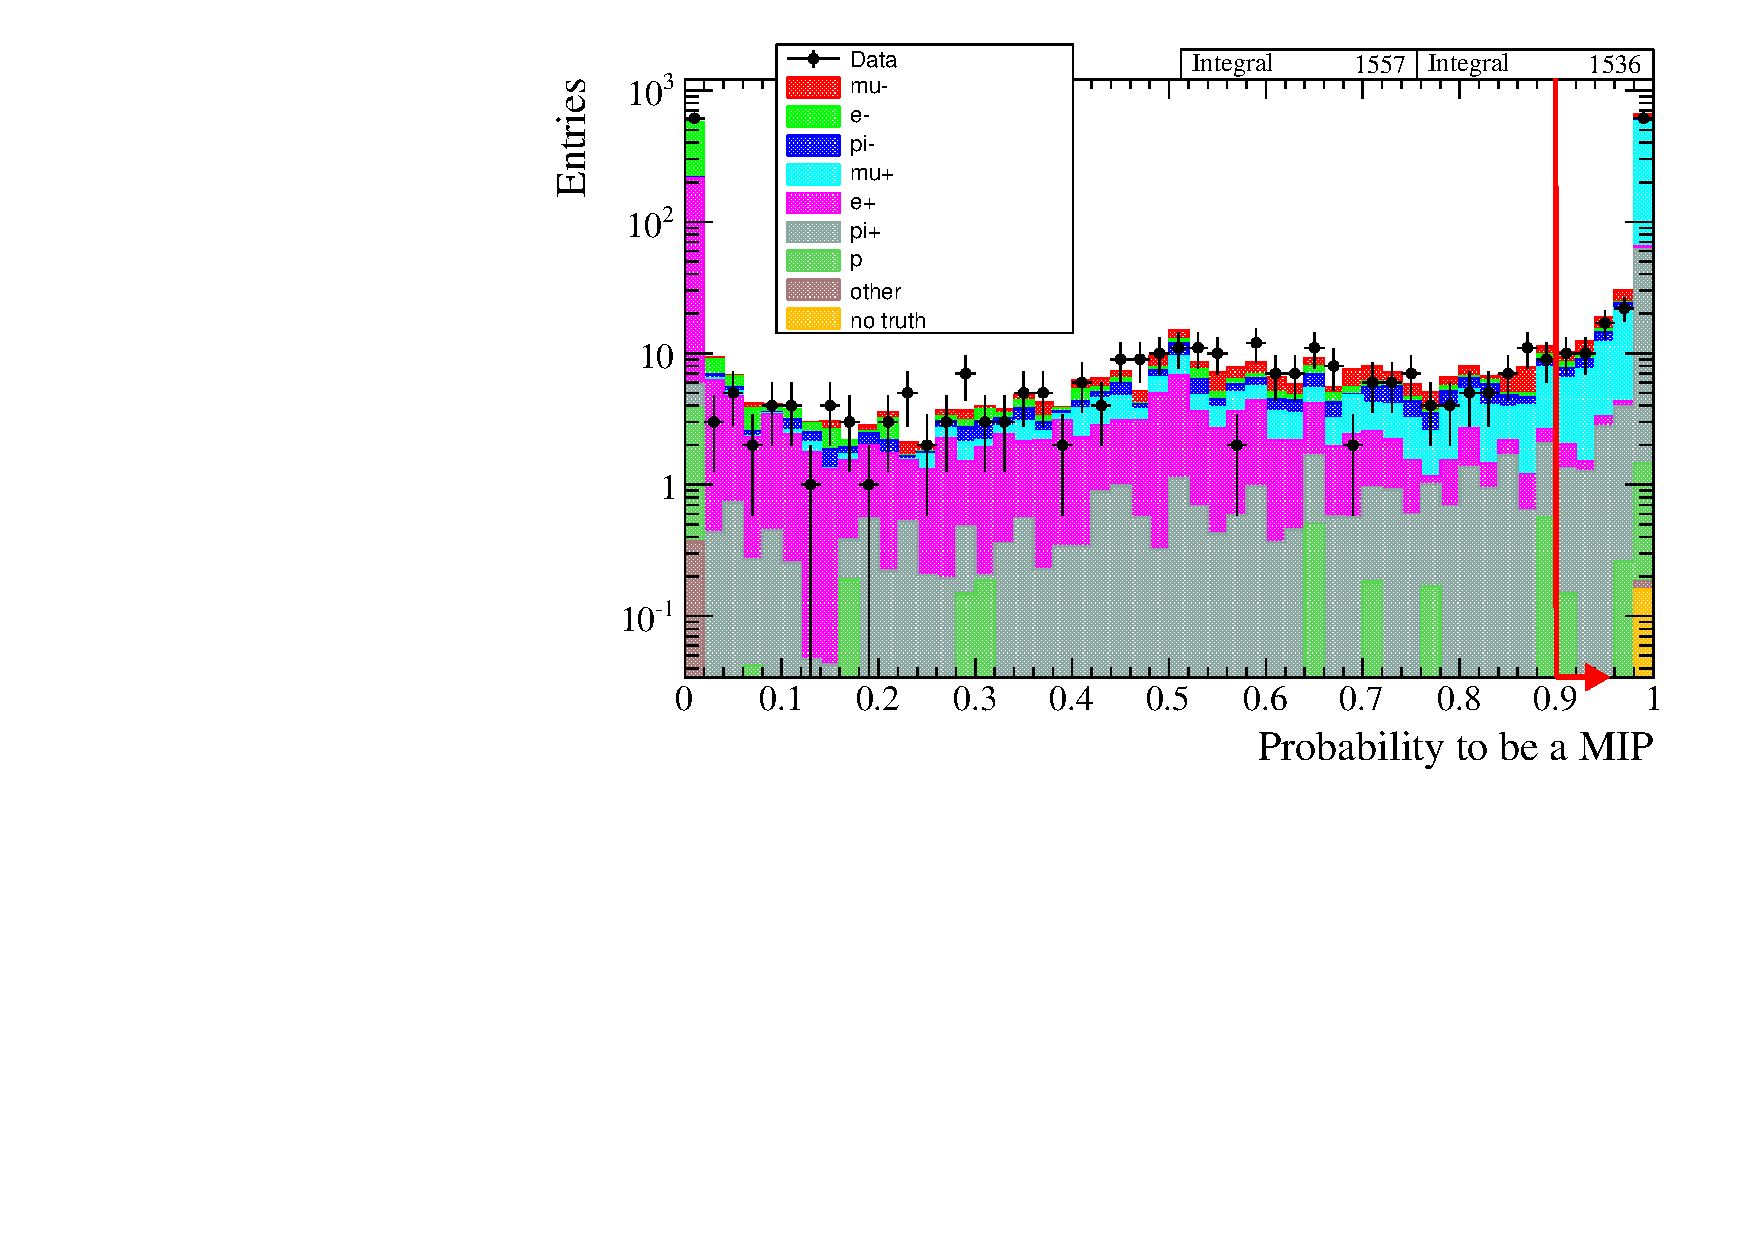
\includegraphics[width=\textwidth]{figures/numu/Cuts/numubar/likemip_numubar}
		\caption{$\mathcal{L}_{MIP}$}
	\end{subfigure}
	\caption{Likelihood distributions for $\mu$ and MIP using run5+6 \numubar data, used in \numubar RHC selections}
	\label{fig:numubar_likelihood}
\end{figure}

\begin{figure}[h]
	\begin{subfigure}[t]{0.49\textwidth}
		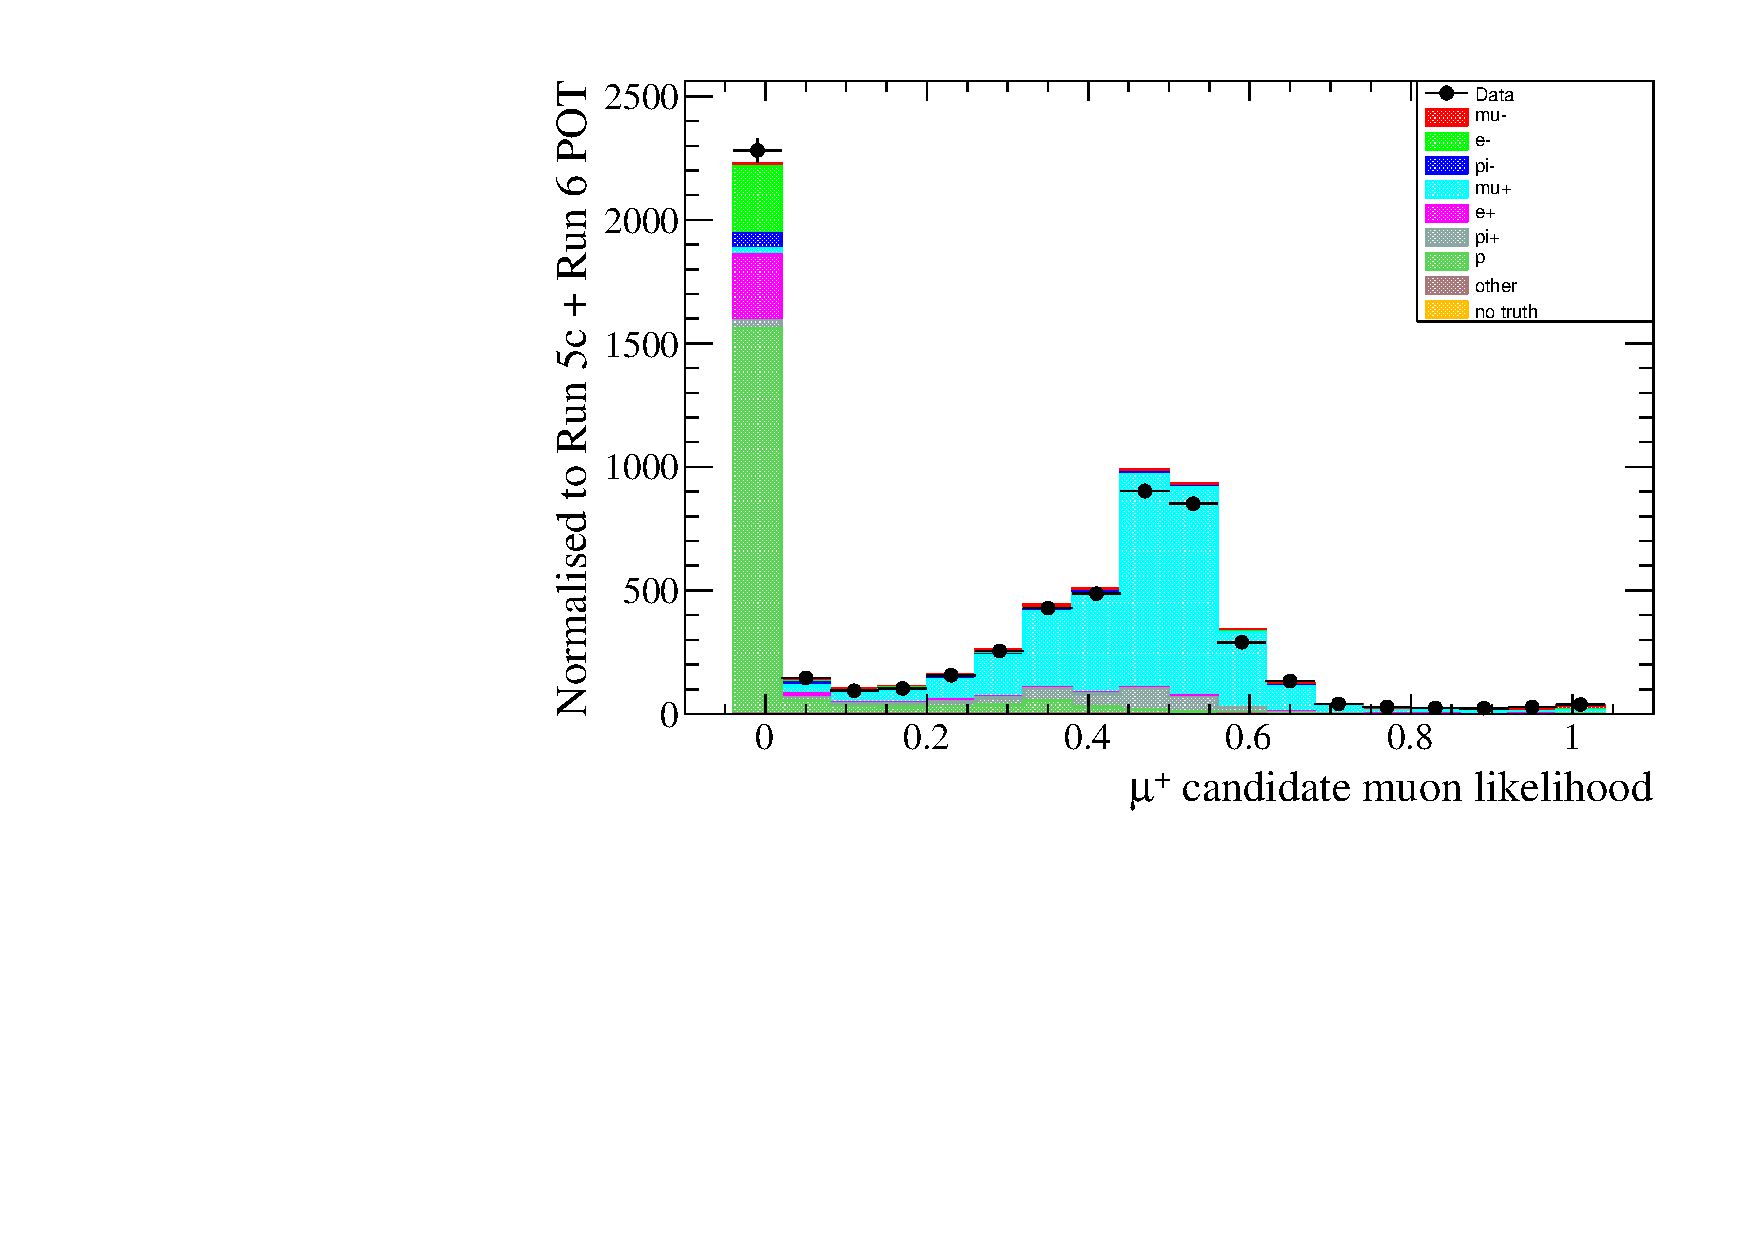
\includegraphics[width=\textwidth]{figures/numu/Cuts/numubar/selmu_likemu_particle}
		\caption{$\mathcal{L}_\mu$}
	\end{subfigure}
	\begin{subfigure}[t]{0.49\textwidth}
		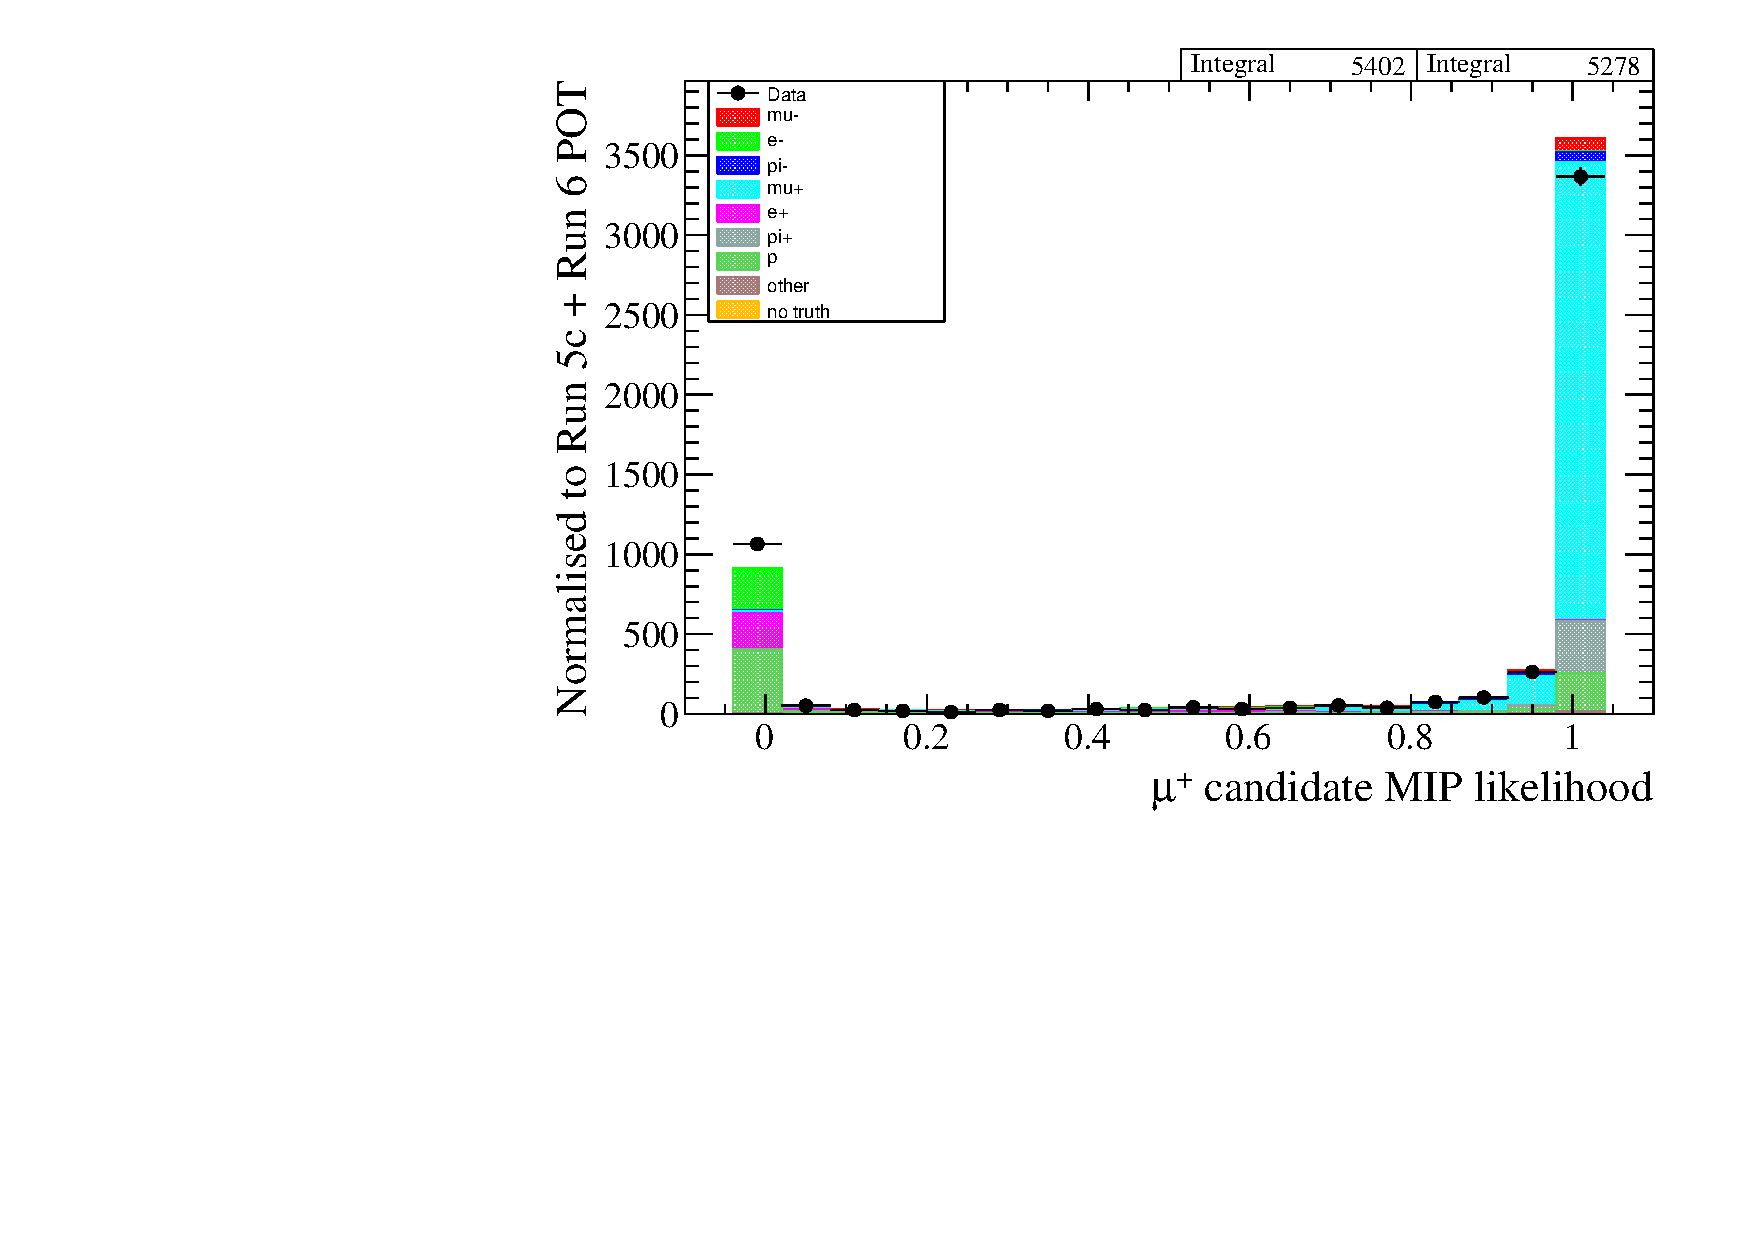
\includegraphics[width=\textwidth]{figures/numu/Cuts/numubar/selmu_likemip_particle}
		\caption{$\mathcal{L}_{MIP}$}
	\end{subfigure}
	\caption{Likelihood distributions for the selected lepton candidate using run5+6 \numubar data, used in \numubar RHC selections}
	\label{fig:numubar_likelihood_sel}
\end{figure}

\begin{figure}[h]
	\begin{subfigure}[t]{0.32\textwidth}
		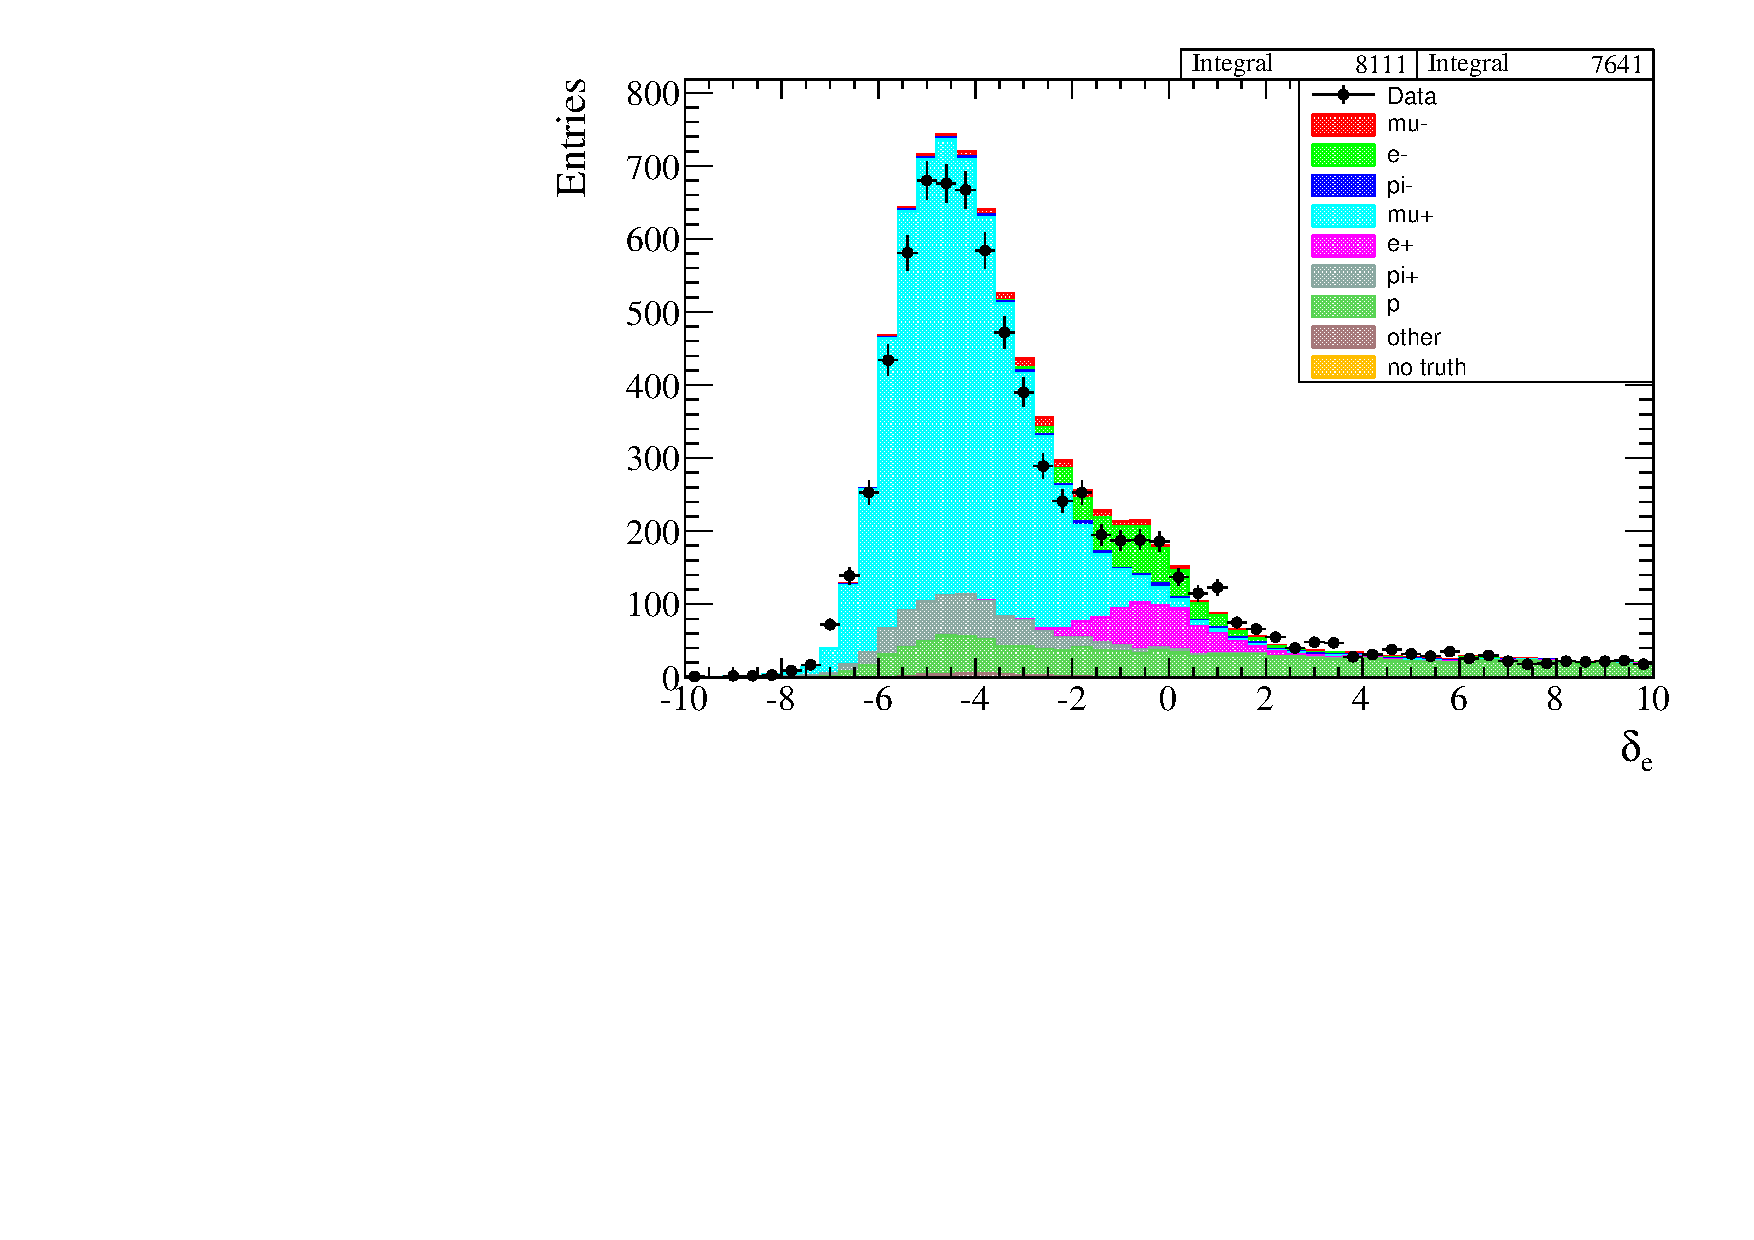
\includegraphics[width=\textwidth]{figures/numu/Cuts/numubar/presel_pullele_part}
		\caption{$\delta_e$}
	\end{subfigure}
	\begin{subfigure}[t]{0.32\textwidth}
		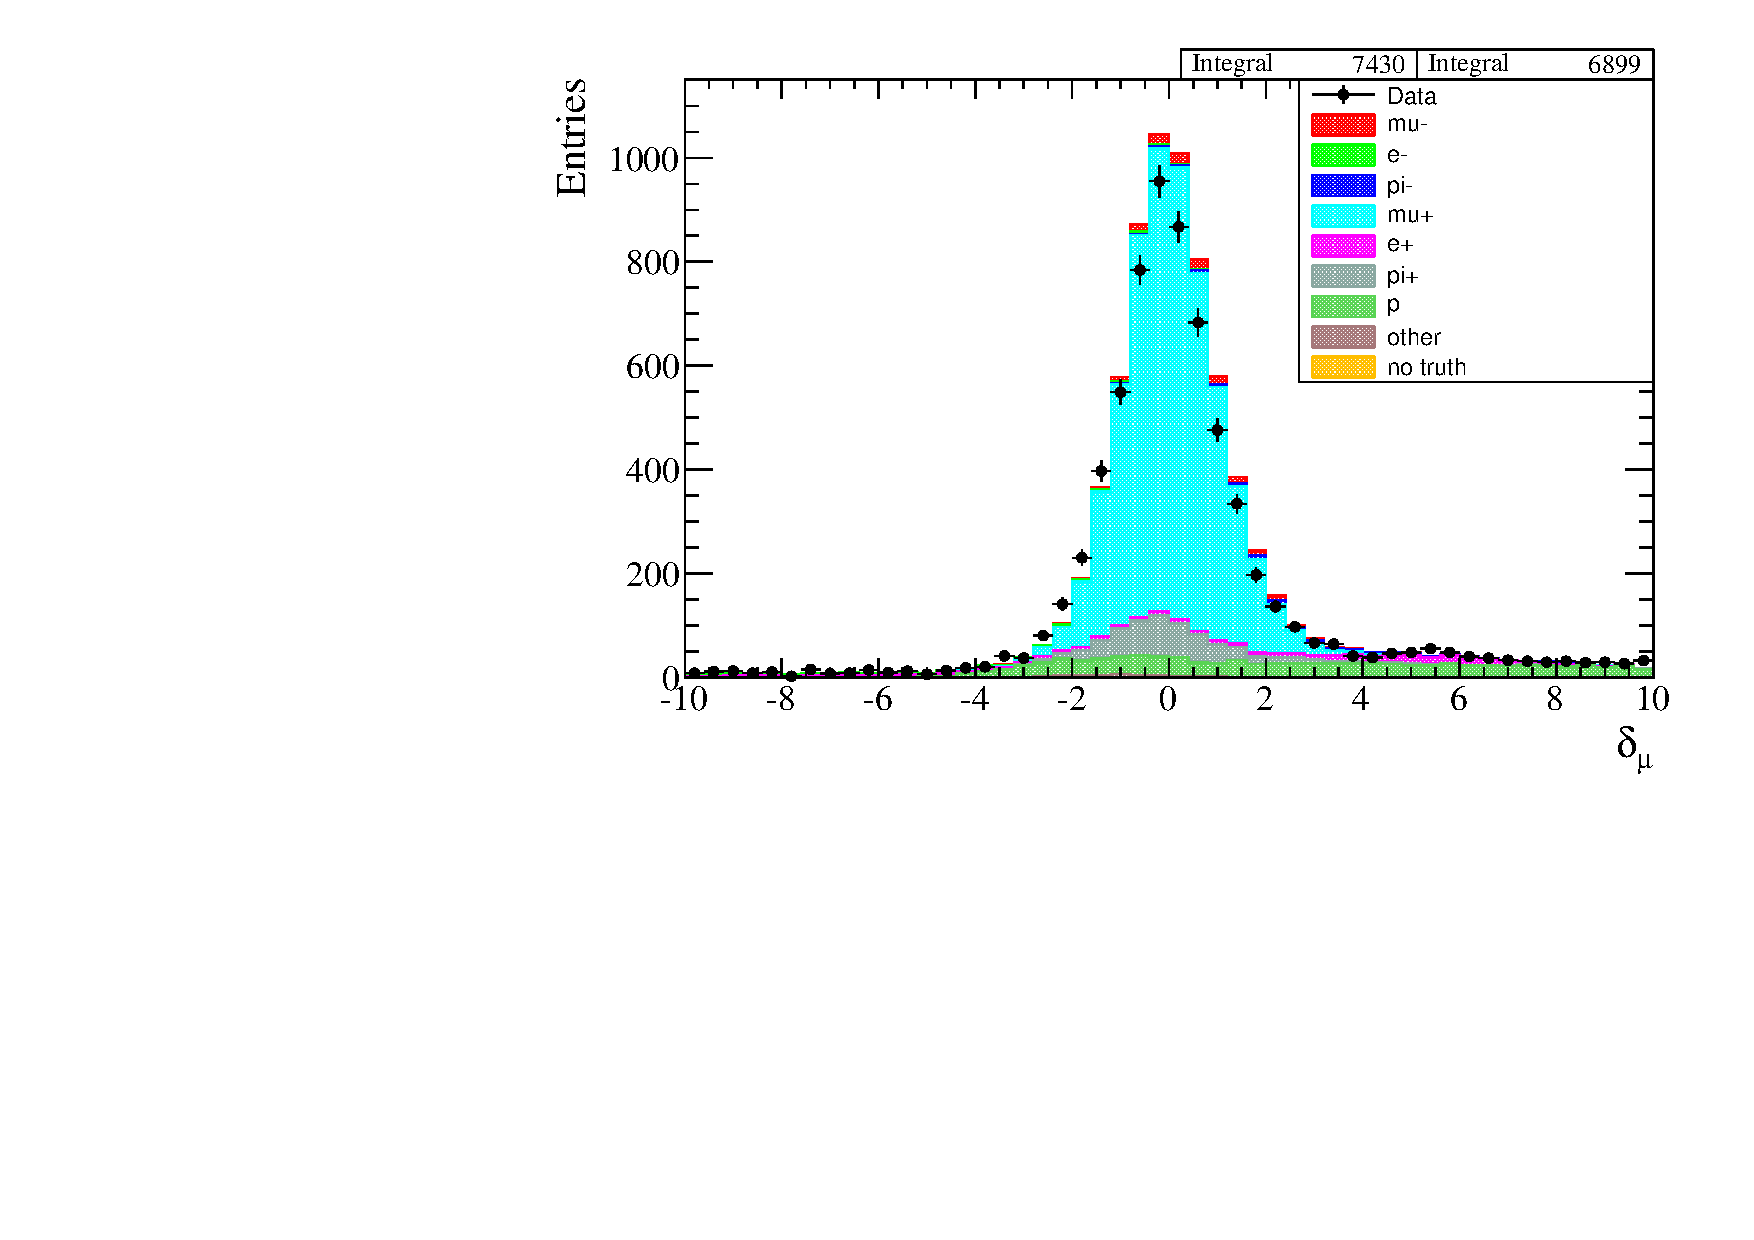
\includegraphics[width=\textwidth]{figures/numu/Cuts/numubar/presel_pullmu_part}
		\caption{$\delta_\mu$}
	\end{subfigure}
	\begin{subfigure}[t]{0.32\textwidth}
		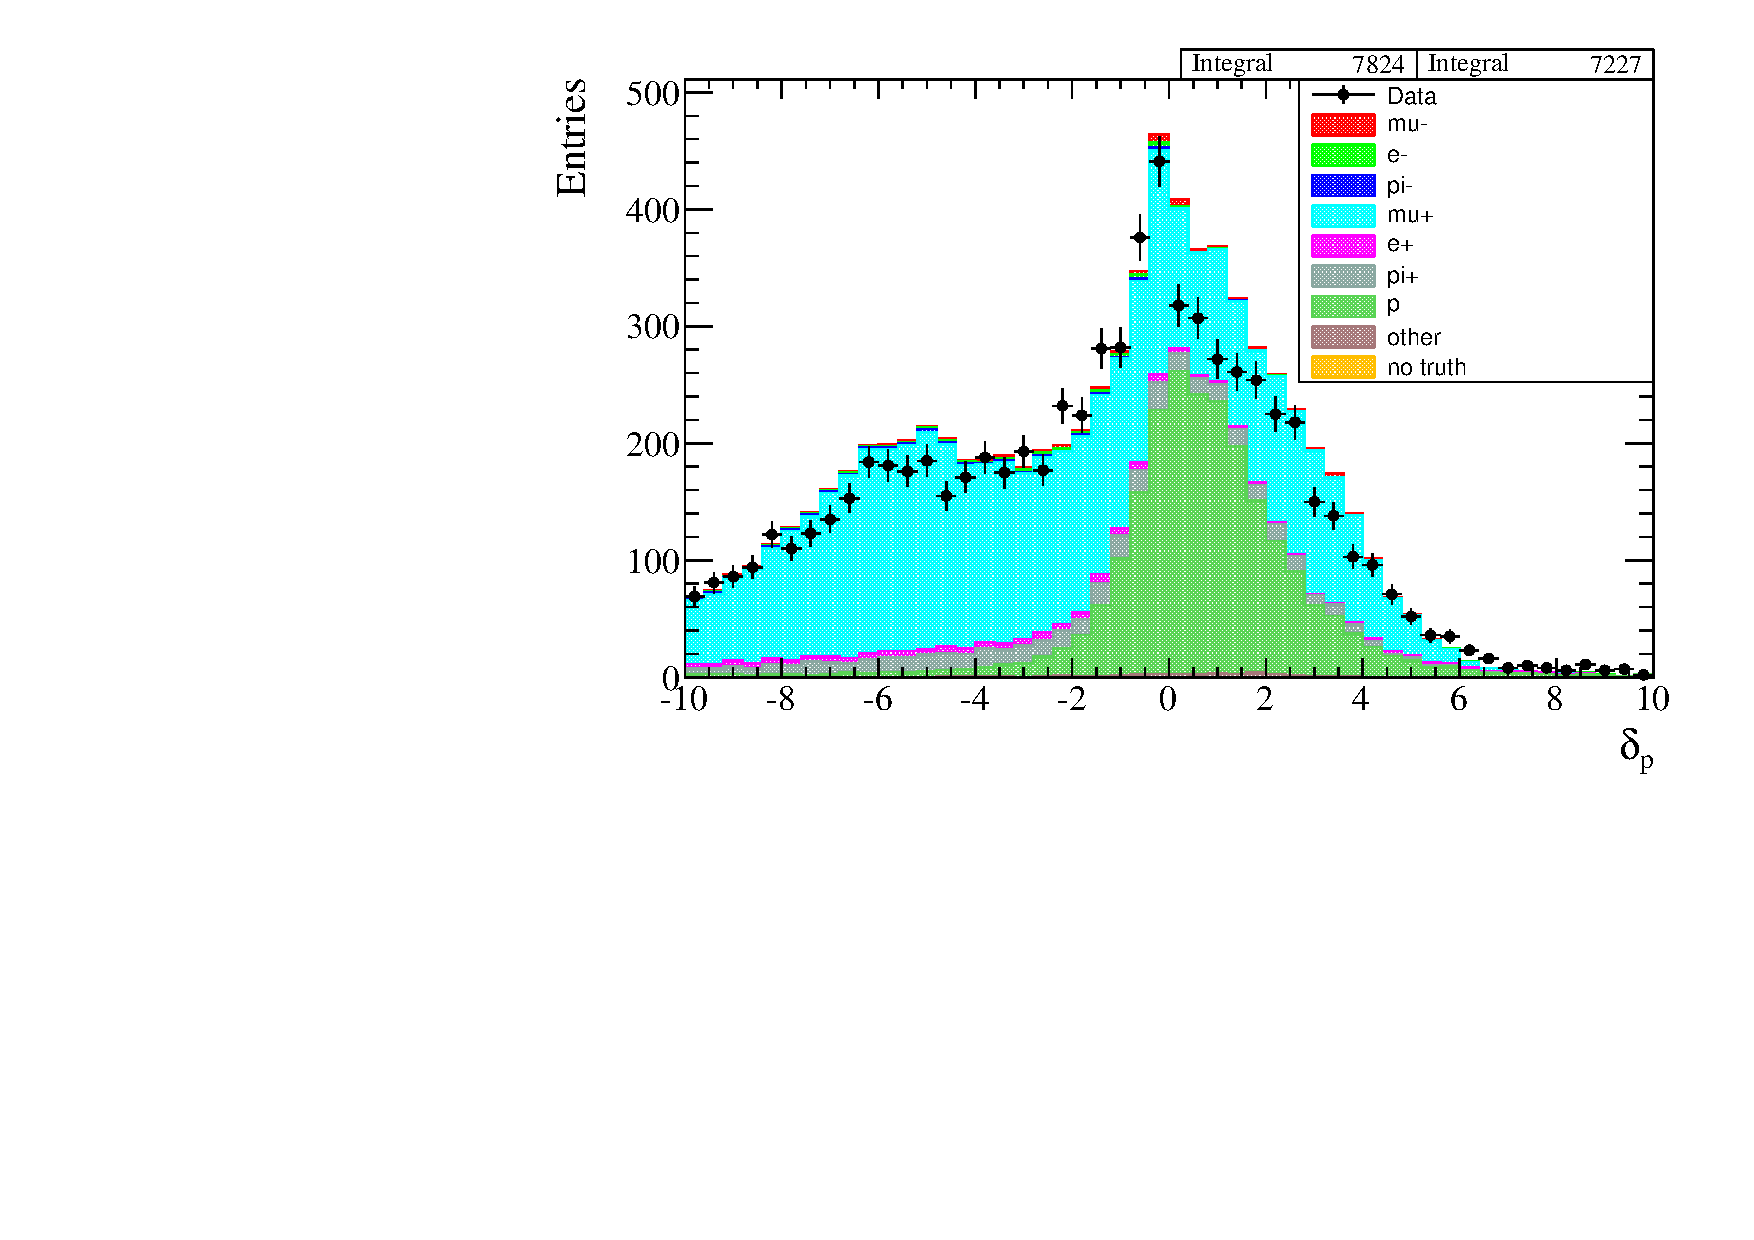
\includegraphics[width=\textwidth]{figures/numu/Cuts/numubar/presel_pullp_part}
		\caption{$\delta_p$}
	\end{subfigure}
	\caption{Pulls ($\delta$) used in the TPC PID used in \numubar RHC selections}
	\label{fig:numubar_pulls}
\end{figure}

Once the \numubar CC-inclusive selection is run the aforementioned pion reconstruction is applied. The \numubar CC1Track selection has one positive muon and does not have any charged or neutral pions in the final state. The \numubar CC1Track selection has a higher efficiency in selecting the muon candidate than the \numu CC0$\pi$ selection from the \numubar resonant interactions producing a $\pi^-$, not a $\pi^+$, which can capture on the nucleus and so do not leave a track to be (falsely) identified as a muon candidate. The \numubar CCNTrack selection contains the remaining particles passing the \numubar CC-inclusive selection, containing at least one neutral or charged pion.

\subsection{\numu in RHC}
\label{sec:numu_in_nubar_sel}
In RHC running there is a large fraction of \numu interactions, owing mostly to the larger \numu cross-section. The same pre-selection cuts are applied for the \numu in RHC selection as for the previous selections.

The CC-inclusive selection proceeds by:
\begin{itemize}
	\item \textbf{Negative multiplicity}: The highest momentum track is required to be the highest momentum negative track, which starts the seeding track. The $\mu^-$ identification uses the TPC PID on the highest momentum negative track. 
	
	\item \textbf{TPC PID}: The PID proceeds by the MIP requirement in \autoref{eq:tpc_track_mip} for particles with $p_\mu < 500 \text{ MeV/c}$, accepting candidate tracks with $\mathcal{L}_{MIP} > 0.7$.
	
	Similar to \autoref{sec:numubar_sel}, a lower and upper bound is set $0.1 < \mathcal{L}_\mu < 0.8$, which rejects protons and low momentum $\mu^+$. The effect of these cuts can be seen in \autoref{fig:nu_numubar_likelihood}.
\end{itemize}

\begin{figure}[h]
	\begin{subfigure}[t]{0.49\textwidth}
		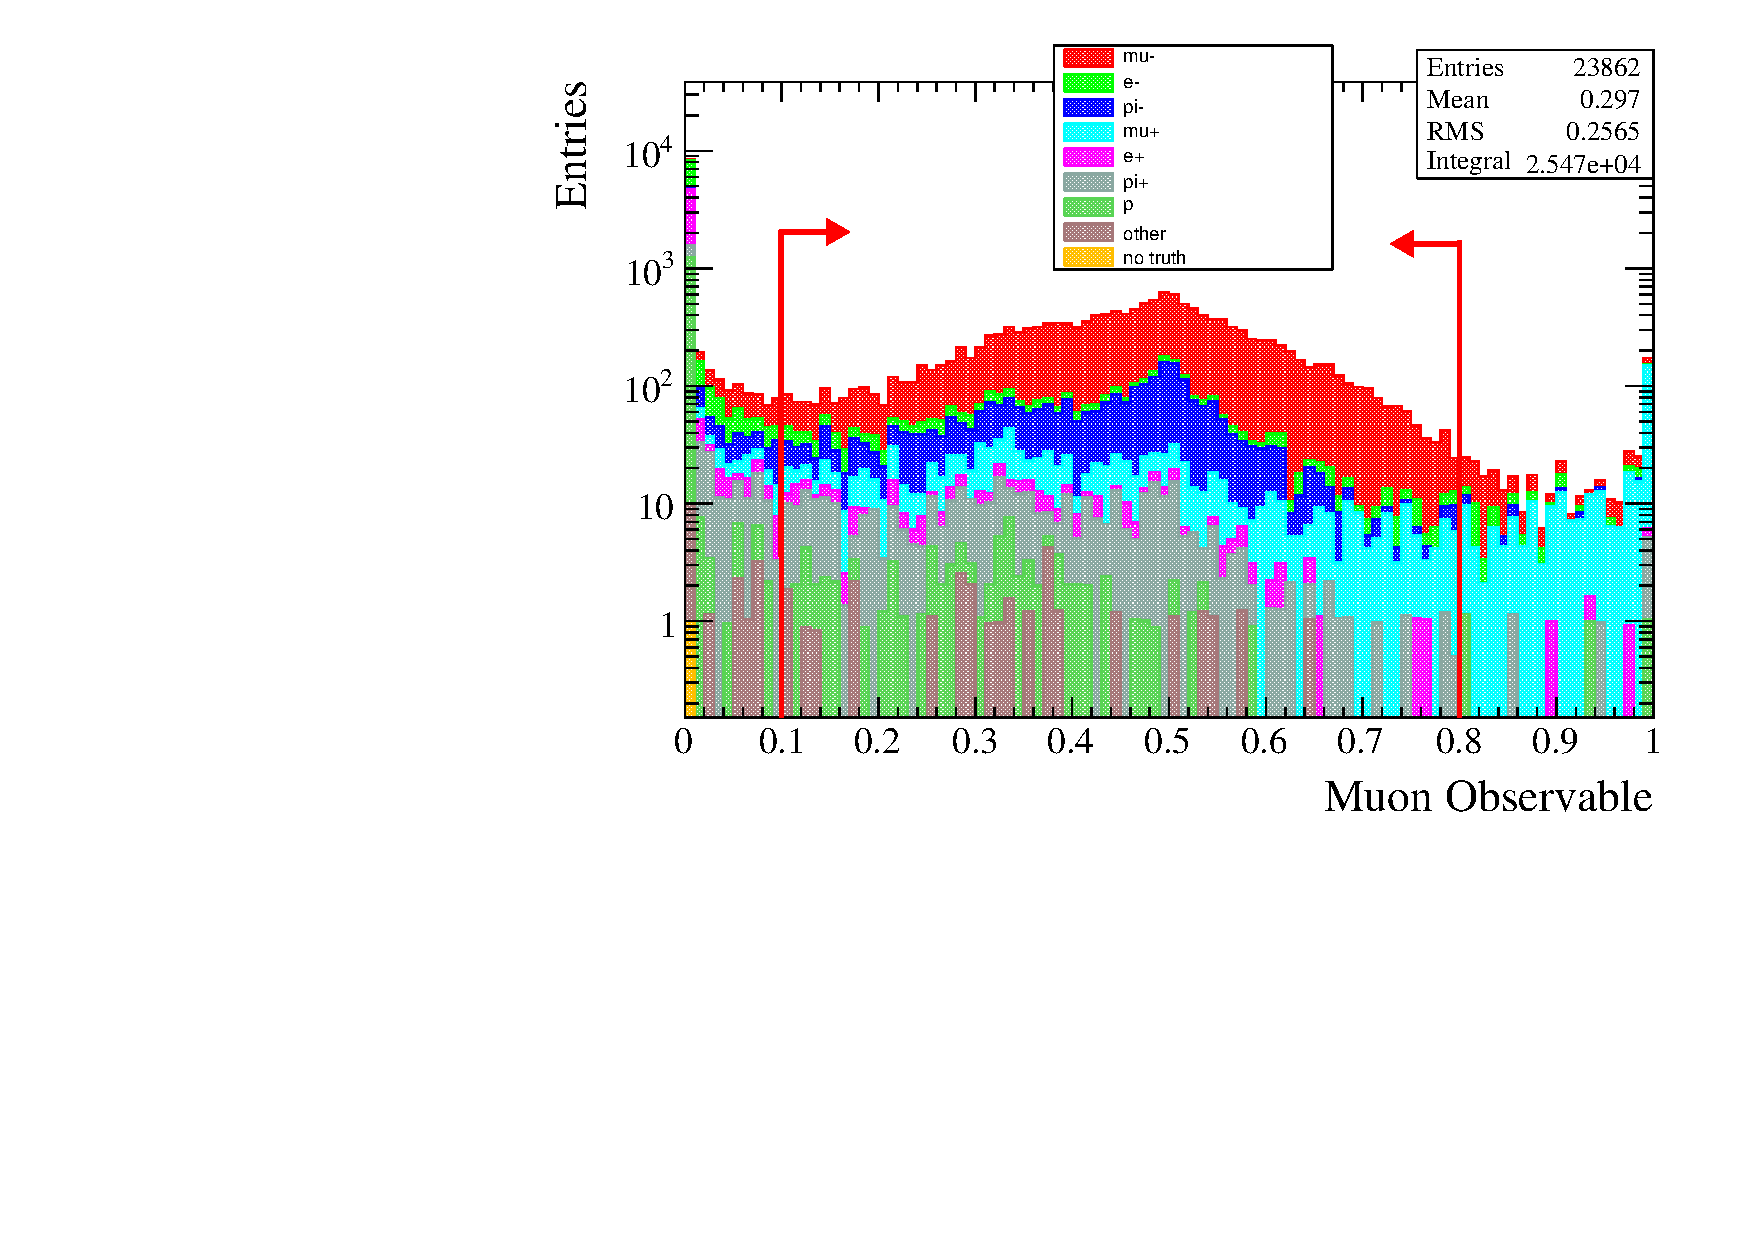
\includegraphics[width=\textwidth]{figures/numu/Cuts/numu_in_numubar/MuonLikelihood_prod6B_NuMuCont_FGD1Only}
		\caption{$\mathcal{L}_\mu$}
	\end{subfigure}
	\begin{subfigure}[t]{0.49\textwidth}
		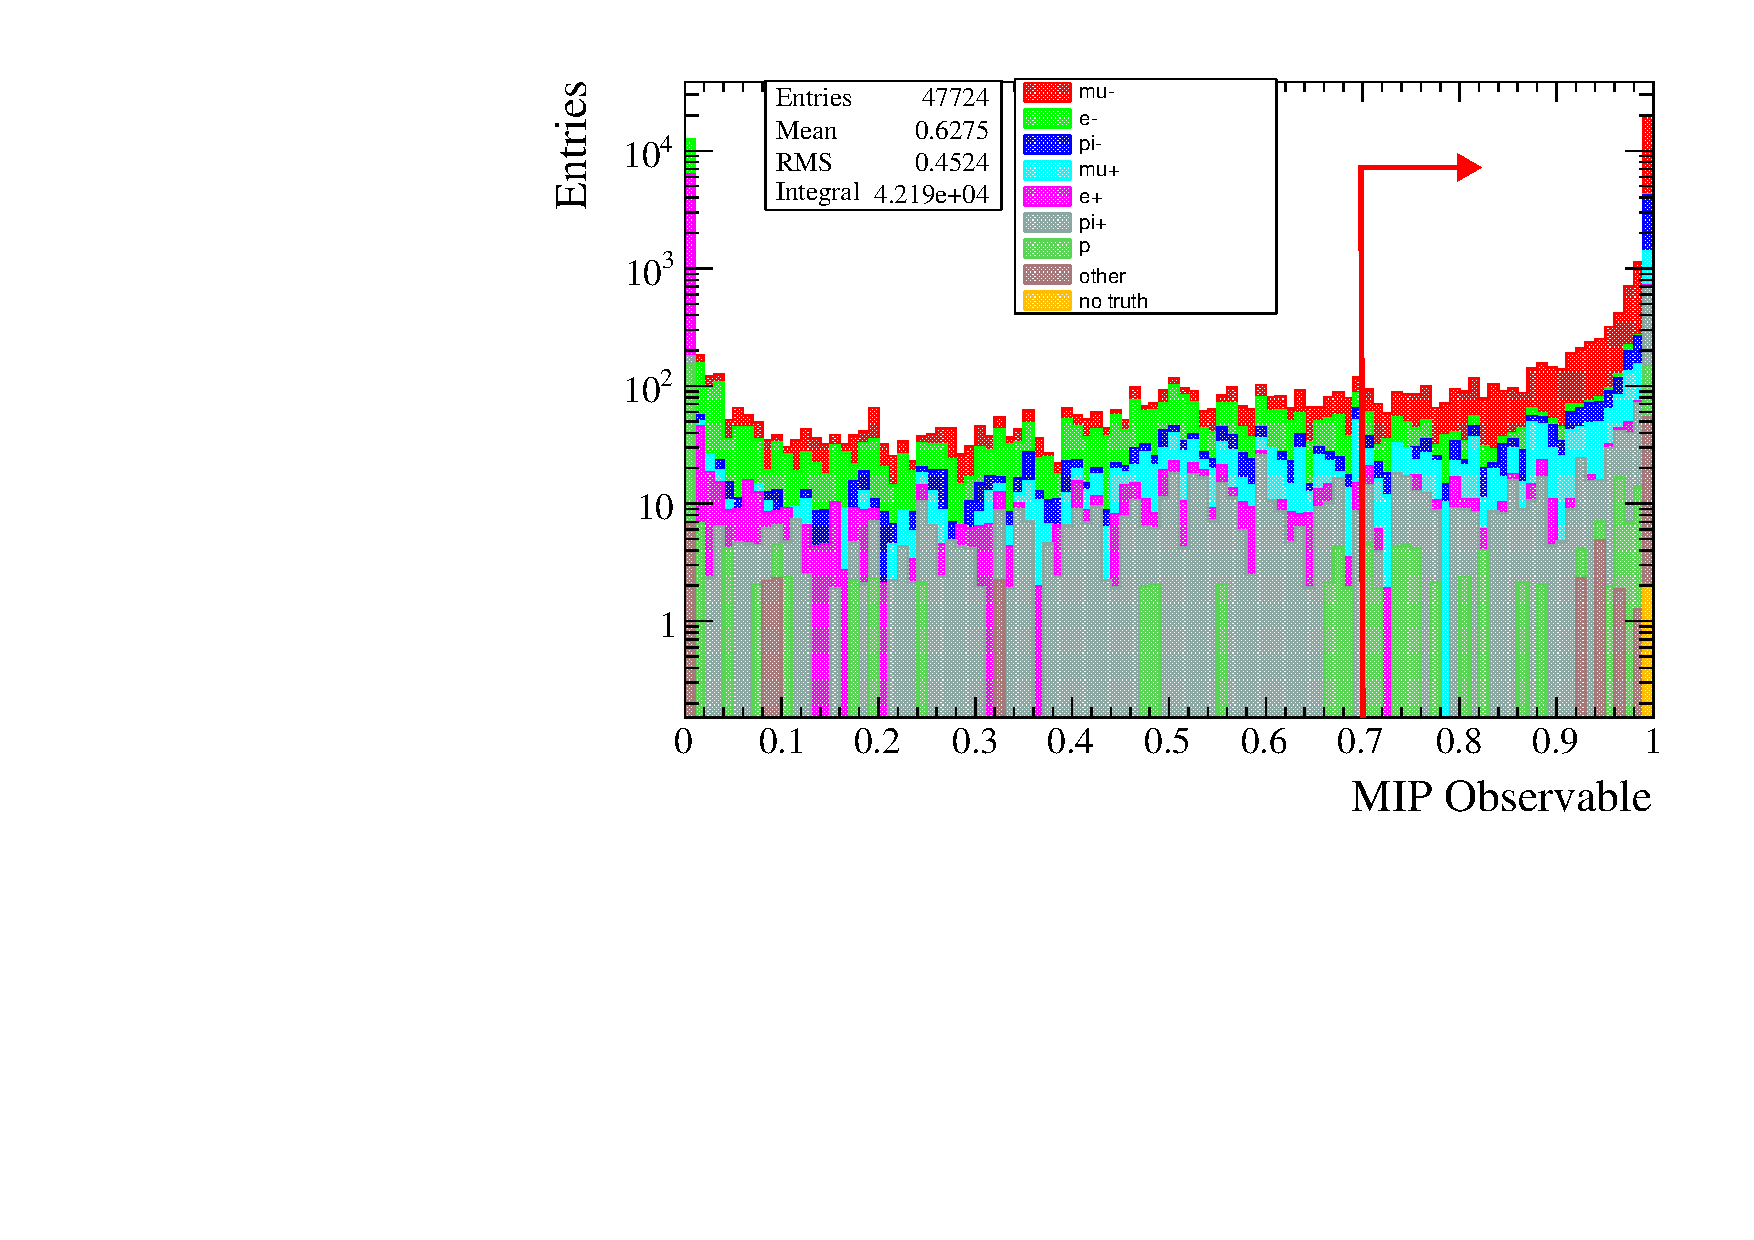
\includegraphics[width=\textwidth]{figures/numu/Cuts/numu_in_numubar/MipLikelihood_LogScale}
		\caption{$\mathcal{L}_{MIP}$}
	\end{subfigure}
	\caption{Likelihood distributions for $\mu$ and MIP using run5+6 \numubar data, used in \numu in RHC selections}
	\label{fig:nu_numubar_likelihood}
\end{figure}

The \numu in RHC selection then breaks down the CC-inclusive selection into CC1Track and CCNTrack, based entirely on the number of TPC-FGD matched tracks. Events with one such reconstructed track enters the CC1Track selection, and events with any other number of tracks regardless of PID, enter the CCNTrack selection. Hence the \numu RHC selection is analogous to the \numubar RHC selection.

A summary of all selections' efficiency and purities is shown in \autoref{tab:eff_pur_summary}. We note $90+\%$ efficiency for CC0$\pi$ and 1 right-sign 1Track efficiencies, with about 75\% purity. As the track multiplicity increases, the efficiencies and purities drop. The NTrack selections in \numubar perform the worst at 55\% efficiency and 45\% purity. For more detail see \autoref{chap:eff_2017}.
\begin{table}[h]
	\centering
	\begin{tabular}{ l | c c }
		\hline
		\hline
		Selection 					   & Efficiency (\%) & Purity (\%) \\ 
		\hline
		\FGDCCNoPi{1}{\numu}           & 93.8  & 75.5  \\% \hline
		\FGDCCNoPi{2}{\numu}           & 93.2  & 73.5  \\% \hline
		\hline
		\FGDCCOnePi{1}{\numu}          & 83.3  & 58.0  \\% \hline
		\FGDCCOnePi{2}{\numu}          & 83.1  & 57.1  \\% \hline
		\hline
		\FGDCCOther{1}{\numu}          & 73.0  & 65.3  \\% \hline
		\FGDCCOther{2}{\numu}          & 73.4  & 64.9  \\% \hline
		\hline
		\FGDCCOneTrk{1}{\numubar}      & 90.0  & 76.7  \\% \hline
		\FGDCCOneTrk{2}{\numubar}      & 89.6  & 76.7  \\% \hline
		\hline
		\FGDCCNTrk{1}{\numubar}   	   & 54.1  & 45.1  \\% \hline
		\FGDCCNTrk{2}{\numubar}        & 53.8  & 43.9  \\% \hline
		\hline
		\FGDCCOneTrk{1}{\numu} in RHC  & 76.5  & 52.2  \\% \hline
		\FGDCCOneTrk{2}{\numu} in RHC  & 74.9  & 51.8  \\% \hline
		\hline
		\FGDCCNTrk{1}{\numu} in RHC    & 73.9  & 60.9  \\% \hline
		\FGDCCNTrk{2}{\numu} in RHC    & 74.2  & 61.4  \\% \hline
		\hline
		\hline
	\end{tabular}
	\caption{Efficiency and purity summary for all selections with the range $0 < p_{reco} < 3\text{ GeV/c}$}
	\label{tab:eff_pur_summary}
\end{table}

\section{Binning the Selections}
\label{sec:binning_2017}
We expect largely similar kinematics across the two FGDs so apply the same binning in reconstructed muon momentum, \pmu, and cosine of the average neutrino-muon angle, \cosmu. The binning for the fit is primarily influenced by MC statistics: we require $\sim 20$ raw MC events per bin (roughly equivalent to 1-2 data events). The momentum resolution is $\sim50\text{ MeV}$ up to 1 GeV and the angular resolution $\sim 2\degree$, seen in \autoref{appendix:detector_resolution}.

The binning in \pmu (MeV/c) \cosmu for each sample is shown below. The FHC selections all have similar binning and has the highest number of bins. The total number of bins is 1624, of which 902 are FHC (six selections) and 722 are RHC (eight selections).
\begin{itemize}
	\item FGD1+2  CC$0\pi$, CC1$\pi$ and CCOther \numu: 154 bins CC0$\pi$, CCOther; 143 bins CC1$\pi$\\
	\pmu: 0, 300, 400, 500, 600, 700, 800, 900, 1000, 1250, 1500, 2000, 3000 (not for CC1$\pi$), 5000, 30000\\
	\cosmu:  -1, 0.6, 0.7, 0.8, 0.85, 0.9, 0.92, 0.94, 0.96, 0.98, 0.99, 1
	
	\item \FGDCCOneTrk{1+2}{\numubar}: 130 bins\\
	\pmu: 0, 400, 500, 600, 700, 800, 900, 1100, 1400, 2000, 10000\\
	\cosmu: -1.0, 0.6, 0.7, 0.8, 0.85, 0.88, 0.91, 0.93, 0.95, 0.96, 0.97, 0.98, 0.99, 1
	
	\item \FGDCCNTrk{1+2}{\numubar}: 77 bins \\
	\pmu: 0, 700, 950, 1200, 1500, 2000, 3000, 10000\\
	\cosmu: -1.0, 0.75, 0.85, 0.88, 0.91, 0.93, 0.95, 0.96, 0.97, 0.98, 0.99, 1
	
	\item \FGDCCnuOneTrk{1+2}{\numu} in RHC: 66 bins\\
	\pmu: 0, 400, 600, 800, 1100, 2000, 10000 \\
	\cosmu: -1.0, 0.7, 0.8, 0.85, 0.9, 0.93, 0.95, 0.96, 0.97, 0.98, 0.99, 1
	
	\item \FGDCCnuNTrk{1+2}{\numu} in RHC: 88 bins\\
	\pmu: 0, 500, 700, 1000, 1250, 1500, 2000, 3000, 10000\\
	\cosmu: -1.0, 0.7, 0.8, 0.85, 0.9, 0.93, 0.95, 0.96, 0.97, 0.98, 0.99, 1
\end{itemize}
  \section{Systematics}
\label{sec:syst}

\epigraph{``The garbage of the past often becomes the treasure of the present (and vice versa)''}{A. M. Polyakov at Gauge Fields and Strings, London, 1987}

The fit aims to constrain systematic parameters for T2K-SK oscillation analyses by using near-detector data. The shared parameters between ND280 and SK are the neutrino flux parameters, and neutrino-nucleus interaction parameters. The nuisance parameters can be considered as the ND280 detector parameters and cross-section parameters that are parametrised as effective on Carbon only. As such, there are many parameters of interest in this analysis, which this section covers.

The systematics enter the fit by changing the predicted event distributions by shape and/or normalisation, which often incur a likelihood penalty for moving parameters away from their prior central values. The penalty takes two forms: either Gaussian or constant. In the case where there is firm reason to believe a parameter is constrained from other sources than ND280 data, the Gaussian penalty is imposed. When external data and/or recent model developments indicate lacking or conflicting knowledge of a parameter, a flat prior is chosen.

For the Gaussian penalty we have
\begin{equation}
	-2\log\mathcal{L}_\text{Penalty} = (X_i-\mu_i) \left(\mathbf{V}\right)^{-1}_{i,j} (X_j-\mu_j)
\end{equation}
for parameter $i$, with current value $X_i$, constant priors $\mu_i$ and covariance matrix $\mathbf{V}$. For a flat penalty instead
\begin{equation}
	-2\log\mathcal{L}_\text{Penalty} = C
\end{equation}
where $C$ is a constant.

\subsection{The Beamline and Neutrino Flux}
\label{subsec:syst_flux}
The flux systematics are split into six categories:
\begin{itemize}
	\item Hadron interaction uncertainties
	\item Proton beam profile and off-axis angle
	\item Horn current and field
	\item Horn and target alignment
	\item Materials modelling
	\item Number of protons on target
\end{itemize}
The simulations are updated each year to improve the modelling, often taking new data in to account. An example is using the dedicated NA61/SHINE T2K replica target data \cite{NA61_pions_rep} to tune the hadron production model at the T2K beam target, and including results from the HARP experiment \cite{harp}.

The fractional errors for the ND280 neutrino flux prediction are shown in \autoref{fig:flux_uncert_fhc} for FHC running and \autoref{fig:flux_uncert_rhc} for RHC running. The uncertainties are $\sim10\%$ in the flux peak region and are dominated by hadron interaction uncertainties, which arise primarily from multiplicity, pion rescattering and interaction length uncertainties. The proton beam profile and off-axis angle become important shortly after the flux peak at about 1 GeV for the right-sign component of the flux.
\begin{figure}[h]
	\begin{subfigure}[t]{0.42\textwidth}
		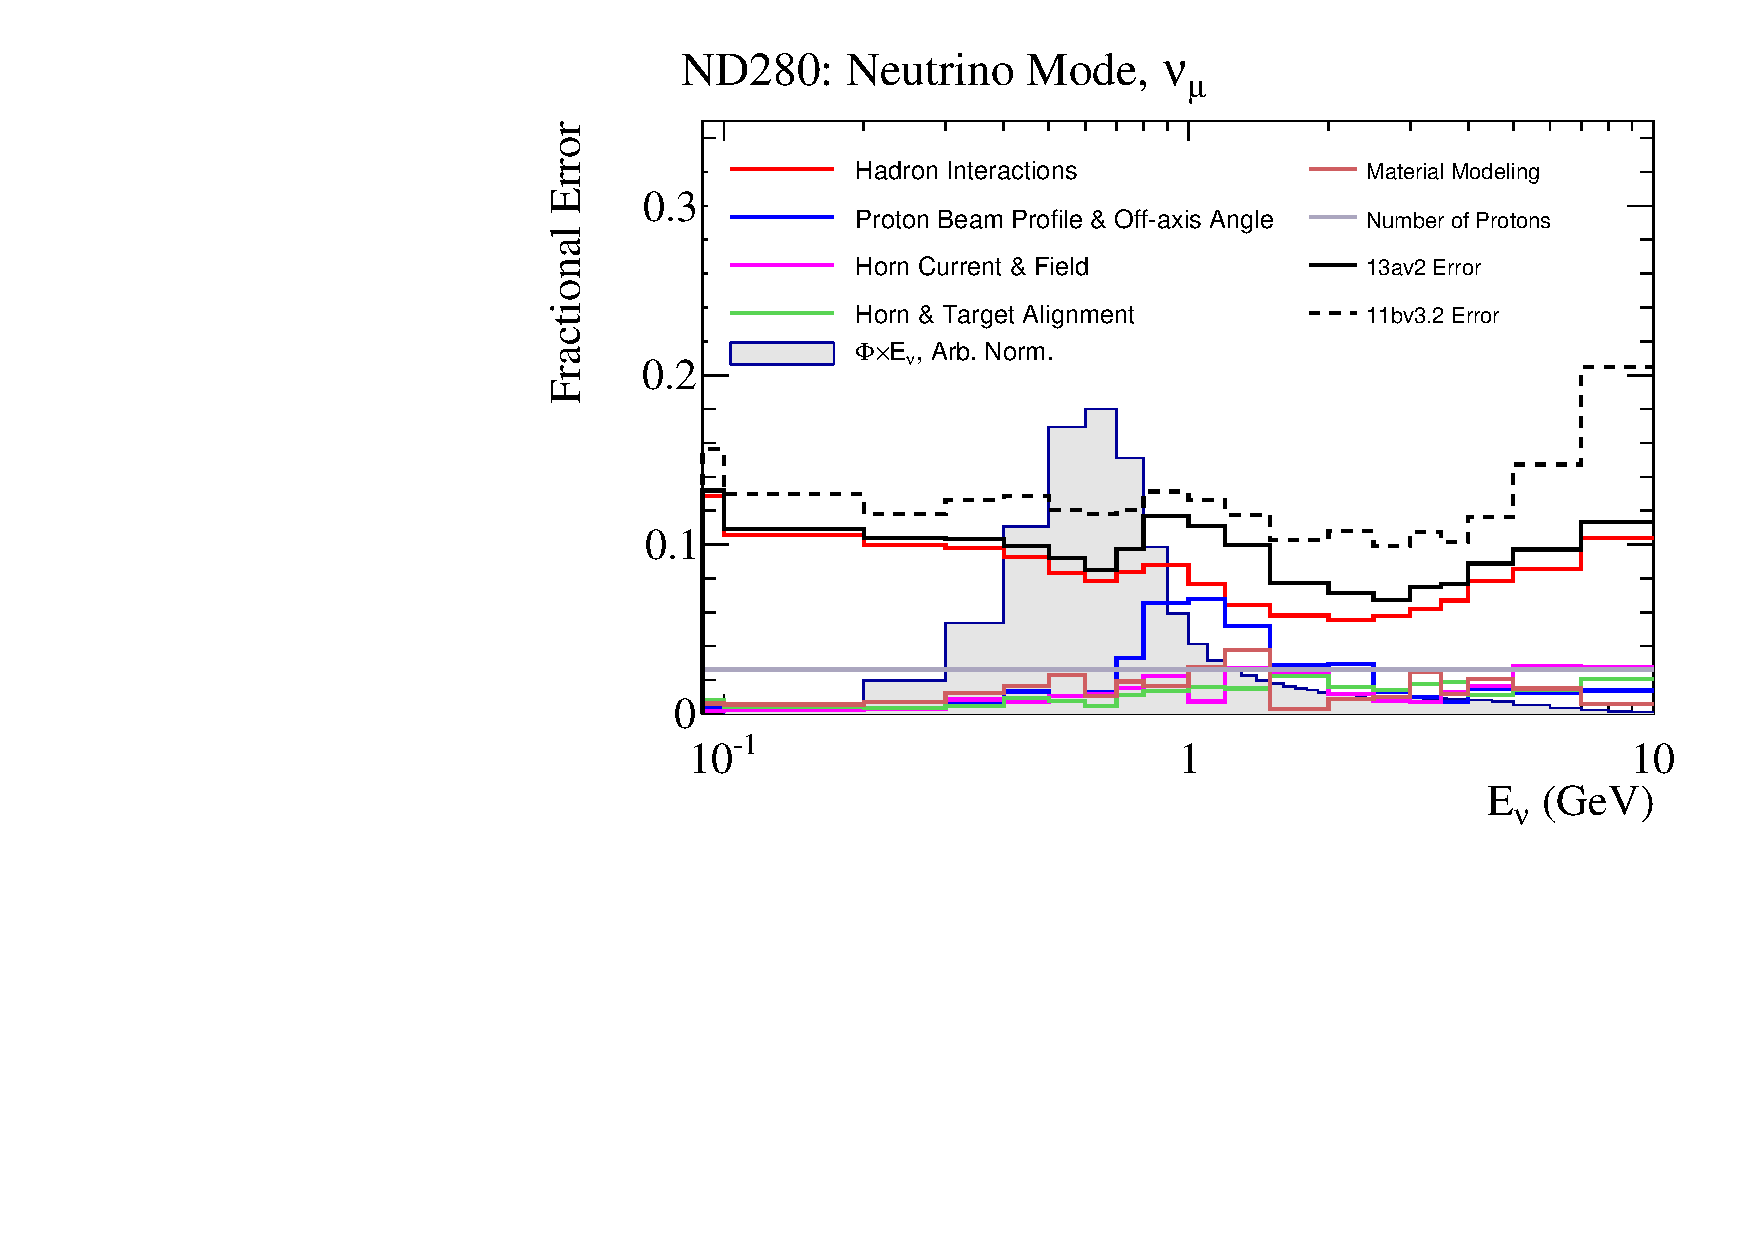
\includegraphics[width=\textwidth, trim={0mm 0mm 0mm 0mm}, clip,page=1]{figures/flux/total_err_nd5_numode_numu}
	\end{subfigure}
	\begin{subfigure}[t]{0.42\textwidth}
		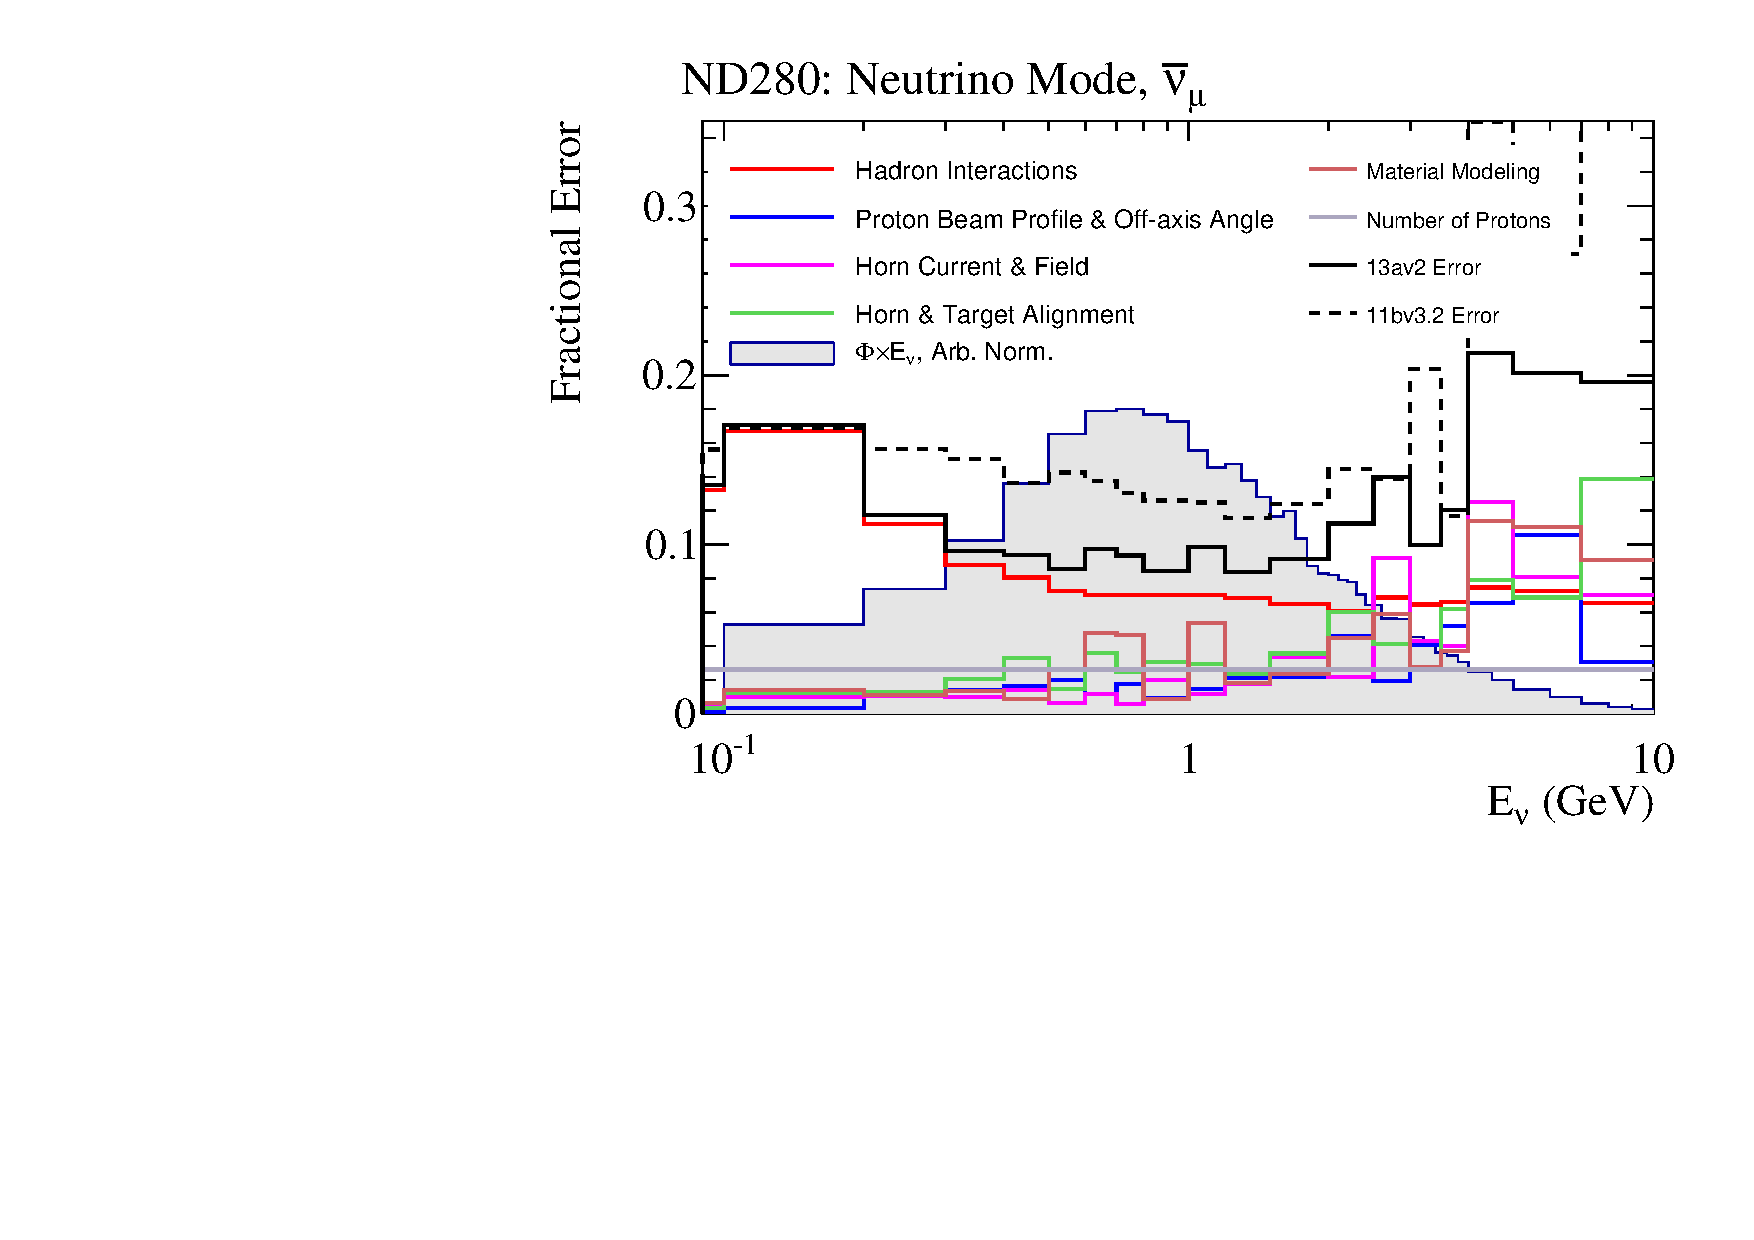
\includegraphics[width=\textwidth, trim={0mm 0mm 0mm 0mm}, clip,page=1]{figures/flux/total_err_nd5_numode_numub}
	\end{subfigure}

	\begin{subfigure}[t]{0.42\textwidth}
		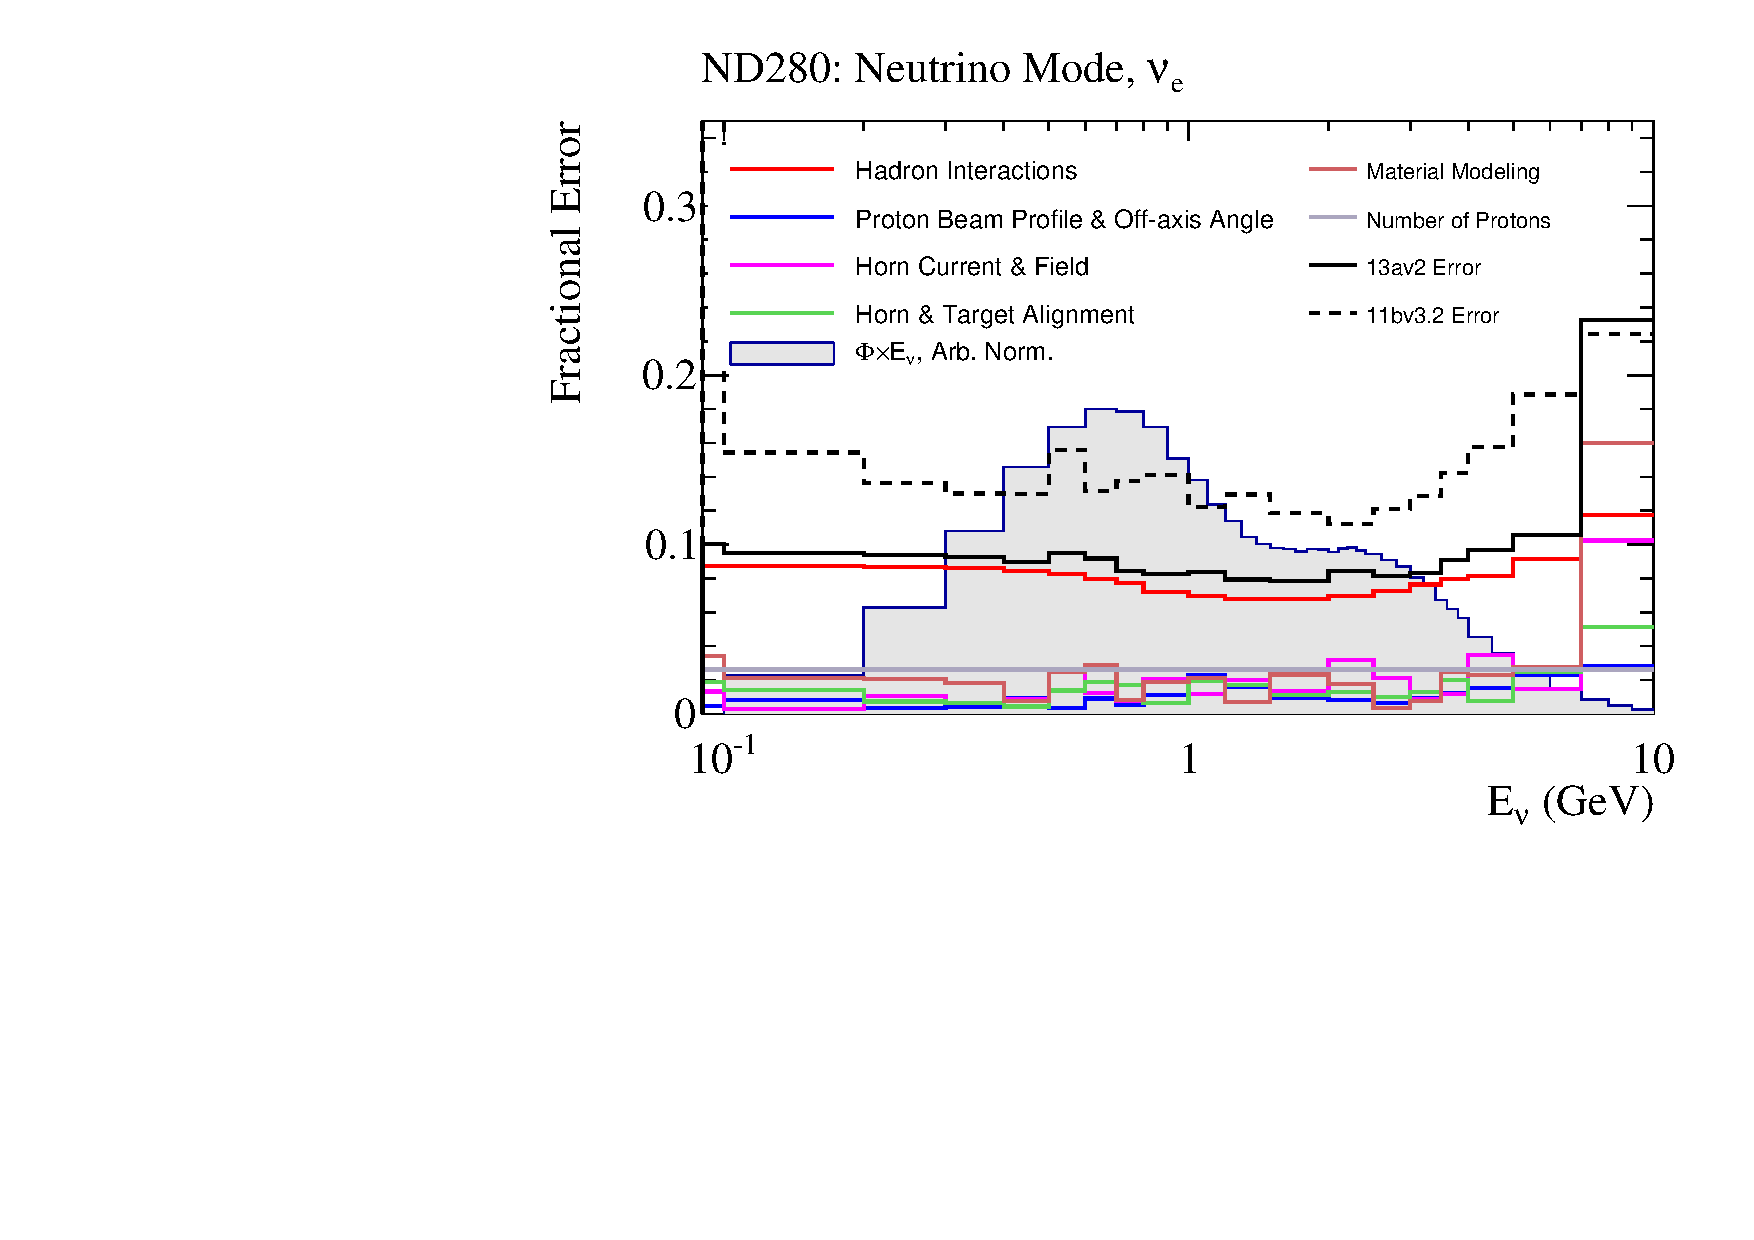
\includegraphics[width=\textwidth, trim={0mm 0mm 0mm 0mm}, clip,page=1]{figures/flux/total_err_nd5_numode_nue}
	\end{subfigure}
	\begin{subfigure}[t]{0.42\textwidth}
		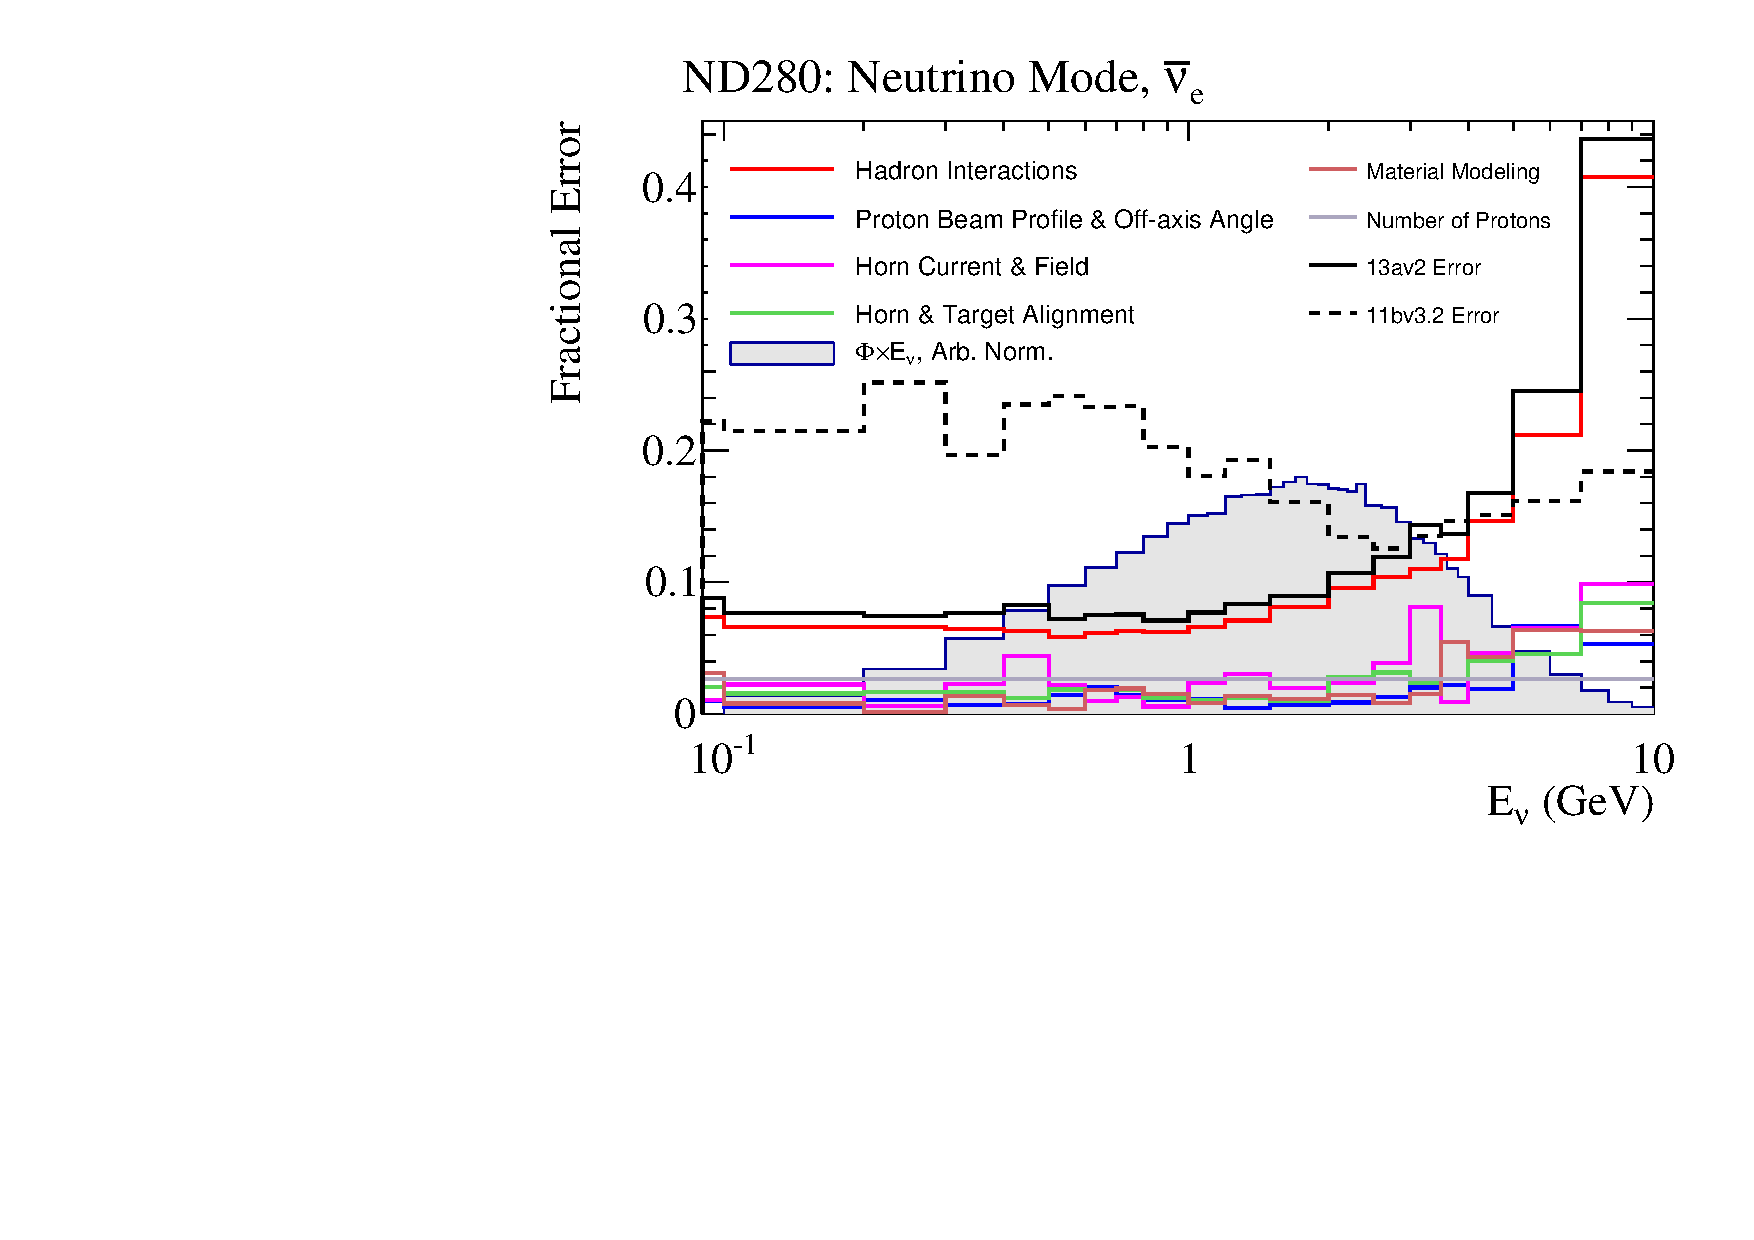
\includegraphics[width=\textwidth, trim={0mm 0mm 0mm 0mm}, clip,page=1]{figures/flux/total_err_nd5_numode_nueb}
	\end{subfigure}
	\caption{FHC flux uncertainties, ``13av2 Error'' is used for this analysis}
	\label{fig:flux_uncert_fhc}
\end{figure}

\begin{figure}[h]
	\begin{subfigure}[t]{0.42\textwidth}
		\includegraphics[width=\textwidth, trim={0mm 0mm 0mm 0mm}, clip,page=1]{figures/flux/total_err_nd5_anumode_numub}
	\end{subfigure}
	\begin{subfigure}[t]{0.42\textwidth}
		\includegraphics[width=\textwidth, trim={0mm 0mm 0mm 0mm}, clip,page=1]{figures/flux/total_err_nd5_anumode_numu}
	\end{subfigure}

	\begin{subfigure}[t]{0.42\textwidth}
		\includegraphics[width=\textwidth, trim={0mm 0mm 0mm 0mm}, clip,page=1]{figures/flux/total_err_nd5_anumode_nue}
	\end{subfigure}
	\begin{subfigure}[t]{0.42\textwidth}
		\includegraphics[width=\textwidth, trim={0mm 0mm 0mm 0mm}, clip,page=1]{figures/flux/total_err_nd5_anumode_nueb}
	\end{subfigure}
\caption{RHC flux uncertainties, ``13av2 Error'' is used for this analysis}
\label{fig:flux_uncert_rhc}
\end{figure}

Importantly, the hadronic interaction uncertainties are reducible by improved modelling and tuning to hadron production data. An example is the black dashed line and the black solid line in \autoref{fig:flux_uncert_fhc}, which shows the reduction in flux uncertainty from 2014 to 2015 analyses. Additionally, new in-situ beam profile monitors aid in reducing the proton beam profile and off-axis angle contributions.

The flux systematics enter the near-detector and oscillation analyses as bin-by-bin normalisations in true neutrino energy, $E_\nu^{true}$ (GeV), for four different neutrino species (\numu, \numubar, \nue, \nuebar), for each running mode (FHC, RHC), for each detector (ND280, SK). The binning is chosen to reflect the magnitude of the neutrino flux and the changing shape but simultaneously keeping the number of parameters relatively low. The right-sign and wrong-sign species have the same binning, so ND280 FHC \numu is binned the same as ND280 RHC \numubar:
\begin{itemize}
	\item ND280, SK FHC \numu; ND280, SK RHC \numubar, :\\
	$E_\nu^{true}$: 0, 0.4, 0.5, 0.6, 0.7, 1, 1.5, 2.5, 3.5, 5, 7, 30
	
	\item ND280, SK FHC \numubar; ND280, SK RHC \numu:\\
	$E_\nu^{true}$: 0, 0.7, 1, 1.5, 2.5, 30
	
	\item ND280, SK FHC \nue; ND280, SK RHC \nuebar:\\
	$E_\nu^{true}$: 0, 0.5, 0.7, 0.8, 1.5, 2.5, 4, 30
	
	\item ND280, SK FHC \nuebar; ND280, SK RHC \nue:\\
	$E_\nu^{true}$: 0, 2.5, 30
\end{itemize}
This procedure brings the total number of flux parameters to 100: 50 for ND280 and 50 for SK. The SK flux parameters are not directly constrained in the ND280-only analysis: the strong correlation between the flux at ND280 and SK indirectly moves SK flux parameters when the ND280 flux parameters move. Hence, all 100 parameters are included in the ND280-only analysis. The flux parameters are highly correlated so the likelihood penalties are evaluated with a covariance matrix, shown in \autoref{fig:flux_cov}.
\begin{figure}[h]
	\includegraphics[width=1.0\textwidth, trim={0mm 0mm 0mm 0mm}, clip,page=1]{figures/mach3/inputs/flux_covariance_banff_13av2}
	\caption{13av2 neutrino flux covariance matrix, used in this analysis}
	\label{fig:flux_cov}
\end{figure}

In addition to the variation systematics above, there is also a nominal flux correction applied to each event as a function of its run period (e.g. run 2a), neutrino specie (e.g. \numubar) and $E_\nu^{true}$ (e.g. 0.8 GeV); this is present to correct the nominal flux model with updated measurements. An example of the corrections from run 4a and run 5b is shown in \autoref{fig:flux_ratio}.
\begin{figure}[h]
	\begin{subfigure}[t]{0.42\textwidth}
		\includegraphics[width=\textwidth, trim={0mm 0mm 0mm 0mm}, clip,page=1]{figures/flux/run4_enu_nd5_13av2_numu_rat}
		\caption{4a \numu}
	\end{subfigure}
	\begin{subfigure}[t]{0.42\textwidth}
		\includegraphics[width=\textwidth, trim={0mm 0mm 0mm 0mm}, clip,page=1]{figures/flux/run5b_enu_nd5_13av2_numubar_rat}
		\caption{5b \numubar}
	\end{subfigure}
	\caption{Nominal flux corrections applied to events interacting in the ND5 (ND280 tracker) plane}
	\label{fig:flux_ratio}
\end{figure}

\subsection{The ND280 Detector}
\label{subsec:syst_nd280}
The treatment of ND280 detector systematic uncertainties consists of varying the underlying detector systematics---such as the TPC PID, FGD PID, and TPC Momentum scale---and study the impact on the number of predicted events in each \pmu, \cosmu bin. 

The parameterisation of near detector systematics are categorised into pure event or selection-changing. The event weighting can be broken down further into efficiencies (with shapes) and normalisation parameters. When FGD-related systematics are concerned---such as pion tagging by Michel electron identification---the two FGDs have separate implementations to account for geometric and compositional differences. The different sources of systematics, their variation type and assumed probability distribution function (PDF) are shown in \autoref{tab:nd280_systs}.
\begin{table}[h]
	\begin{tabular}{l | c c}
	\hline
	\hline
	Systematic						& Variation 	& PDF \\
	\hline
	\multicolumn{3}{l}{\textbf{TPC}} \\
	Magnetic Field Distortions		& Observable 	& Flat \\
	TPC Momentum Scale				& Observable	& Gauss \\
	TPC Momentum Resolution			& Observable	& Gauss \\
	TPC PID							& Observable	& Gauss \\
	TPC Cluster Efficiency			& Efficiency	& Gauss \\
	TPC Tracking Efficiency			& Efficiency	& Gauss \\
	TPC Charge ID Efficiency		& Efficiency	& Gauss \\
	\hline 
	\multicolumn{3}{l}{\textbf{FGD-TPC}} \\
	TPC-FGD Matching Efficiency		& Efficiency	& Gauss \\
	\hline
	\multicolumn{3}{l}{\textbf{FGD}} \\
	FGD PID							& Observable	& Gauss \\
	FGD1-FGD2 Time of Flight		& Observable	& Gauss \\
	FGD Hybrid Tracking Efficiency	& Efficiency	& Gauss \\
	Michel Electron Efficiency		& Efficiency	& Gauss \\
	\hline
	\multicolumn{3}{l}{\textbf{Backgrounds}} \\
	Out-of-Fiducial-Volume			& Normalisation & Gauss \\
	Sand Muons						& Normalisation & Gauss \\
	Pile-Up							& Normalisation	& Gauss \\
	\hline
	\multicolumn{3}{l}{\textbf{MC modelling}} \\
	Pion secondary interactions		& Normalisation & Gauss \\
	FGD Mass						& Normalisation & Gauss \\
	\hline
	\hline
	\end{tabular}
\caption{ND280 systematics present in the fit}
\label{tab:nd280_systs}
\end{table}

\paragraph{Observable Variation Systematics}
This group of systematics have the potential to change the reconstructed topology, so allow for migration in and out of selections. They can also switch the reconstructed lepton candidate to a different track in the event. The systematic is applied as a smearing to the reconstructed event variables (e.g. \pmu, \cosmu) and then reruns the event selection algorithm on the smeared event.

There are two methods with which the smearing is applied:
\begin{itemize}
	\item If the relevant reconstructed variable has a known true value, the difference between the two is used as a scaling. The updated value of the variable after the variation is then
	\begin{equation}
		x'_{reco} = x_{true} + \left(x_{reco}^{MC}-x_{true}\right)\left(s + \alpha \cdot \delta s\right)
	\end{equation}
	where $\alpha$ is the random variable from the relevant systematic's PDF in \autoref{tab:nd280_systs}, $s$ is the scaling factor, and $\delta s$ is its statistical error. The scaling factor is defined as
	\begin{equation}
		s = \frac{\sigma^{data}}{\sigma^{MC}}
	\end{equation}
	and
	\begin{equation}
		\delta s = s \cdot \left| \frac{\delta \sigma^{data}}{\sigma^{Data}} - \frac{\delta \sigma^{MC}}{\sigma^{MC}} \right|
	\end{equation}
	where $\sigma^{data}$ is the dispersion observed in data and $\delta \sigma^{data}$ is the error on the dispersion.
	\item If the MC is corrected to match a data mean value. This correction is needed because the effect of a systematic error ($\delta \Delta \bar{x}$) on the selected event relative the nominal MC is not guaranteed to agree with the corrected MC. The updated observable is then
	\begin{equation}
		x'_{reco} = x^{MC}_{reco}+ \Delta\bar{x} + \alpha \delta \Delta \bar{x}
	\end{equation}
	where $\Delta\bar{x} = \bar{x}^{data}_{reco}-\bar{x}^{MC}_{reco}$ and $\bar{x}_{reco}$ is the mean value of the variable $x$, $\alpha$ is a random variable, and $\delta \Delta \bar{x}$ is the associated uncertainty from the reconstructed data and MC discrepancy,
	\begin{equation}
		\delta \Delta \bar{x} = \sqrt{\Delta\bar{x}^2 + \left(\delta \bar{x}^{data}_{reco}\right)^2  + \left(\delta \bar{x}^{MC}_{reco}\right)^2}
	\end{equation}
\end{itemize}

Additionally uncertainties from the magnetic field are special cases of the above:
\begin{itemize}
	\item The TPC laser calibration corrections are used on-top of the B-field mapping corrections, where the latter is applied during reconstruction and the former is treated as an uncertainty. The reconstructed variable is then
	\begin{equation}
		x'_{reco} = x^{MC}_{reco} + \alpha \left(x_{reco}^{New}-x_{reco}^{MC}\right)
	\end{equation}
	where $\alpha$ is the random variable and $x_{reco}^{New}$ is the reconstructed momentum after the updated mapping is applied. This applies to the magnetic field distortion systematic.
	\item If the observable depends on a scale $s$ that is easy to extract from in-situ measurements
	\begin{equation}
		x'_{reco} = x_{reco}^{MC}+\alpha \delta x
	\end{equation}
	where $\delta x = x_{reco}^{MC} \delta s$ is the uncertainty on the observable and $\delta s$ is the uncertainty on the scaling variable. The TPC momentum scale systematic uses this parameterisation, in which $s$ is the scale of the magnet current and $\delta s$ is its uncertainty.
\end{itemize}

\paragraph{Efficiency Systematics}
The weight systematics are computed from studies which compare data and MC predictions in well known control samples. The multiple ND280 subdetectors enable cross-checks for tracking and matching efficiencies: e.g. TPC2 tracking efficiency can be computed using tracks with segments in FGD1 and FGD2, which therefore should also have a track in TPC2 which can be cross-checked.

Using the sand muon control sample---defined as having a through-going muon track in most of the detector, where the muon was created in the surrounding sand in the ND280 pit or the magnet---as an example, such muons tend to be very forward-going and high energy. Thus the sample is suitable for alignment studies but not efficiency studies since the \pmu, \cosmu phase space is very limited. 

The model used to move to some new phase space assumes the ratio between efficiencies in data and MC are the same in analysis and control samples. The efficiency for the data is then
\begin{equation}
\epsilon_{data} = \frac{\epsilon_{data}^{Control}}{\epsilon_{MC}^{Control}} \epsilon_{MC}
\end{equation}
where $\epsilon^{Control}$ is the efficiency in the control sample(s). The statistical uncertainty in $r^{Control} = \epsilon^{Control}_{data}/\epsilon^{Control}_{MC}$ is taken into account as
\begin{equation}
\delta r^{Control} = \sqrt{\left(1-r^{Control}\right)^2 + \left(\delta r^{Control}_{Stat}\right)^2}
\end{equation}
yielding the predicted efficiency in the data as
\begin{equation}
\epsilon_{data}' = \left(r^{Control} + \alpha \delta r^{Control}\right)\epsilon_{MC}
\end{equation}
where $\alpha$ is the random variable. Finally we define the two weights
\begin{equation}
w_{Eff} = \frac{\epsilon_{data}'}{\epsilon_{MC}}
\end{equation}
for events that identify the track correctly and
\begin{equation}
w_{Ineff} = \frac{1-\epsilon_{Data}'}{1-\epsilon_{MC}}
\end{equation}
to propagate the weight systematics on an event-by-event basis.

\paragraph{Normalisation Systematics}
These systematics are simple one-time weights which change the overall event numbers. The FGD mass error is an example of such a systematic: if the mass of the FGD is larger than the nominal, the overall number of observed events in MC should be increased. The weight $w$ is applied as
\begin{equation}
w = 1+\alpha \cdot \delta e
\end{equation}
where 1.0 is the nominal weight, $\alpha$ is a random variable, and $\delta e$ is the systematic error on the source.

\paragraph{Relative Systematic Error Sizes}
\autoref{tab:nd280_syst_error_nu} shows the relative errors from ND280 systematics contribution on the number of predicted events for the different ND280 \numu selections for FGD1. The total error for the CC0$\pi$ selection is 1.66\%, CC1$\pi$ is 3.33\% and CCOther 6.47\%. For comparison, the flux and cross-section errors are generally $\mathcal{O}\left(10\%\right)$. The error increases with selection because the increased track multiplicity and lower ``cleanliness'' of the reconstructed events. 

The largest contribution to the total error is pion secondary interactions, making up $\sim90\%$ of the detector systematics. This systematic has the power to migrate events through selections by changing the number of reconstructed pions. For the CCOther selection the TPC tracking efficiency also has a large contribution (1.79\%), decreasing to 0.44\% for CC1$\pi$ and 0.27\% for CC0$\pi$. The FGD mass contributes 0.6\% uncertainty for all selections, making up 1/3 of the error on CC0$\pi$ selection. FGD2 has similarly sized systematic contributions, although slightly modified due to the geometry: e.g. the sand muon error is smaller in FGD2 due to tighter vetos than in FGD1.
\begin{table}[h]
	\begin{tabular}{l | c c c}
		\hline
		\hline
		Systematic & \multicolumn{3}{c}{Percentage error} \\
				   & CC0$\pi$ & CC1$\pi$ & CCOther \\ 
		\hline	
		\multicolumn{4}{l}{\textbf{TPC}} \\
		Magnetic Field Distortions		& 0.025 & 0.063 & 0.072 \\
		TPC Momentum Scale				& 0.062 & 0.074 & 0.230 \\
		TPC Momentum Resolution			& 0.055 & 0.094 & 0.286 \\
		TPC PID							& 0.316 & 0.792 & 0.616 \\
		TPC Cluster Efficiency			& 0.000 & 0.000 & 0.002 \\
		TPC Tracking Efficiency			& 0.259 & 0.440 & 1.786 \\
		TPC Charge ID Efficiency		& 0.178 & 0.270 & 0.473 \\
		\hline 
		\multicolumn{4}{l}{\textbf{FGD-TPC}} \\
		TPC-FGD Matching Efficiency		& 0.148 & 0.270 & 0.605 \\
		\hline
		\multicolumn{4}{l}{\textbf{FGD}} \\
		FGD PID							& 0.011 & 0.034 & 0.015 \\
		FGD1-FGD2 Time of Flight		& 0.034 & 0.070 & 0.017 \\
		FGD Hybrid Tracking Efficiency	& 0.106 & 0.100 & 0.532 \\
		Michel Electron Efficiency		& 0.062 & 0.253 & 0.008 \\
		\hline
		\multicolumn{4}{l}{\textbf{Backgrounds}} \\
		Out-of-Fiducial-Volume			& 0.391 & 0.541 & 0.286 \\
		Sand Muons						& 0.069 & 0.085 & 0.031 \\
		Pile-Up							& 0.112 & 0.112 & 0.112 \\
		\hline
		\multicolumn{4}{l}{\textbf{MC modelling}} \\
		Pion secondary interactions		& 1.433 & 3.173 & 6.118 \\
		FGD Mass						& 0.595 & 0.595 & 0.595 \\
		\hline
		Total & 1.660 & 3.329 & 6.467 \\
		\hline
		\hline
	\end{tabular}
\caption{Integrated systematic errors for FGD1 FHC related systematics}
\label{tab:nd280_syst_error_nu}
\end{table}

\autoref{tab:nd280_syst_error_nubar} shows the error table for the RHC selections. The tracking related systematics for the FGD (Michel electron tagging, PID, hybrid tracking) are not present because the number of tracks in the event---defining the 1Trk or NTrk selection---is solely based on the number of TPC tracks present, so has no impact.

The largest systematic by far is the pion secondary modelling (90+\%), as is also the case for FHC selections. The impact is larger than for FHC selections since the source of pions are \numu interactions (typically higher in $E_\nu$ so also higher in multiplicity) and the larger uncertainties on $\pi^-$ re-interaction probabilities. The FGD mass is the second largest systematic for CC0$\pi$, although for the CCNTrk selection the TPC tracking efficiency comes in second, followed by the TPC PID, followed by the FGD mass.
\begin{table}[h]
	\begin{tabular}{l | c c}
		\hline
		\hline
		Systematic & \multicolumn{2}{c}{Percentage error} \\
				   & CC1Trk & CCNTrk \\ 
		\hline	
		\multicolumn{3}{l}{\textbf{TPC}} \\
		Magnetic Field Distortions		& 0.004 & 0.165 \\
		TPC Momentum Scale				& 0.049 & 0.246 \\
		TPC Momentum Resolution			& 0.041 & 0.123 \\
		TPC PID							& 0.307 & 0.544 \\
		TPC Cluster Efficiency			& 0.000 & 0.002 \\
		TPC Tracking Efficiency			& 0.436 & 1.201 \\
		TPC Charge ID Efficiency		& 0.117 & 0.115 \\
		\hline 
		\multicolumn{3}{l}{\textbf{FGD-TPC}} \\
		TPC-FGD Matching Efficiency		& 0.109 & 0.394 \\
		\hline
		\multicolumn{3}{l}{\textbf{FGD}} \\
		FGD1-FGD2 Time of Flight		& 0.016 & 0.009 \\
		\hline
		\multicolumn{3}{l}{\textbf{Backgrounds}} \\
		Out-of-Fiducial-Volume			& 0.336 & 0.610 \\
		Sand Muons						& 0.153 & 0.248 \\
		Pile-Up							& 0.240 & 0.241 \\
		\hline
		\multicolumn{3}{l}{\textbf{MC modelling}} \\
		Pion secondary interactions		& 4.902 & 9.198 \\
		FGD Mass						& 0.598 & 0.584 \\
		\hline
		Total 							& 5.371 & 10.378 \\
		\hline
		\hline
	\end{tabular}
	\caption{Integrated systematic errors for FGD1 RHC related systematics}
	\label{tab:nd280_syst_error_nubar}
\end{table}

\paragraph{Parameterisation of ND280 Systematics}
The systematics in \autoref{tab:nd280_systs} could theoretically be varied on an event-by-event basis. In practice this is unfeasible because: 1) the event selection framework is not sufficiently optimised to guarantee fast reweighting; 2) some values of variation systematics gave rise to discontinuous test-statistics as events migrated from one topology to another. Whereas the former is purely computational, the latter causes problems for finding minima with gradient descent algorithms, employed by the other ND280 fitting group (BANFF). 

The systematics are instead parameterised similarly to the flux systematics, which ensures both smoothness and fast reweighting. The systematics listed in \autoref{tab:nd280_systs} are varied on an event-by-event basis and 500 random variations are chosen according to the prior covariances, and the number of events are binned in the fit-binning from \autoref{sec:binning_2017}. The content of each bin is then treated as a normalisation parameter which is highly correlated with adjacent bins through a covariance matrix. Finally, an MC statistical covariance matrix and a covariance matrix shifting the MC reconstructed lepton momentum of CCQE events by 20 MeV to roughly emulate the differences in Martini and Nieves' 1p1h model to the NEUT CCQE model are added\cite{t2k_2015}. The central value and uncertainty on the number of events in a bin comes from a the arithmetic mean and the central value is the rms, and a cross-check with a Gaussian fit is done.

Using the fit binning in \pmu \cosmu yields 1624 ND280 parameters, which was reduced to 556 by merging bins with similar features in the underlying bin-by-bin event distributions. The final ND280 detector matrix binning was chosen to be
\begin{itemize}
	\item FHC $\nu_{\mu}$~CC0$\pi$ bin edges: \\
	\pmu (MeV/c): 0, 1000, 1250, 2000, 3000, 5000, 30000 \\
	\cosmu:  -1, 0.6, 0.7, 0.8, 0.85, 0.94, 0.96, 1
	\item FHC $\nu_{\mu}$~CC1$\pi$  bin edges: \\
	\pmu (MeV/c):  0, 300, 1250, 1500, 5000, 30000 \\
	\cosmu: -1, 0.7, 0.85, 0.9, 0.92, 0.96, 0.98, 0.99, 1
	\item FHC $\nu_{\mu}$~CCOther bin edges: \\
	\pmu (MeV/c): 0, 1500, 2000, 3000, 5000, 30000 \\
	\cosmu:  -1, 0.8, 0.85, 0.9, 0.92, 0.96, 0.98, 0.99, 1
	\item RHC $\bar{\nu}_{\mu}$~CC 1-Track bin edges: \\
	\pmu (MeV/c): 0, 400, 900, 1100, 2000, 10000 \\
	\cosmu:  -1, 0.6, 0.7, 0.88, 0.95, 0.97, 0.98, 0.99, 1.00
	\item RHC $\bar{\nu}_{\mu}$~CC N-Track bin edges: \\
	\pmu (MeV/c):  0, 700, 1200, 1500, 2000, 3000, 10000 \\
	\cosmu: -1, 0.85, 0.88, 0.93, 0.98, 0.99, 1.00
	\item RHC $\nu_{\mu}$~CC 1-Track bin edges: \\
	\pmu (MeV/c):  0, 400, 800, 1100, 2000, 10000 \\
	\cosmu:   -1, 0.7, 0.85, 0.90, 0.93, 0.96, 0.98, 0.99, 1.00
	\item RHC $\nu_{\mu}$~CC N-Track bin edges: \\
	\pmu (MeV/c):  0, 1000, 1500, 2000, 3000, 10000 \\
	\cosmu: -1, 0.8, 0.90, 0.93, 0.95, 0.96, 0.97, 0.99, 1.00
\end{itemize}
in which we note a large first momentum bin for many selections. This is primarily because the pion secondary interaction systematic is by far dominant, which generally becomes larger at higher \pmu (which in turn correlates with higher $E_\nu$), leading to enough energy to create a pion. Reducing the ND280 detector systematic binning had no discernible effect for flux or interaction parameters in a fit to mock data.

\begin{figure}[h]
	\begin{subfigure}[t]{0.42\textwidth}
		\includegraphics[width=\textwidth, trim={4mm 3mm 2mm 2mm}, clip,page=1]{figures/numu/syst/bad_bin}
		\caption{FGD1 CC0$\pi$, 1250-2000, 0.6-0.7}
	\end{subfigure}
	\begin{subfigure}[t]{0.42\textwidth}
		\includegraphics[width=\textwidth, trim={4mm 3mm 2mm 2mm}, clip,page=1]{figures/numu/syst/decent_bin}
		\caption{FGD1 CC1Trk, 0-400, 0.97-0.98}
	\end{subfigure}

	\begin{subfigure}[t]{0.42\textwidth}
		\includegraphics[width=\textwidth, trim={4mm 3mm 2mm 2mm}, clip,page=1]{figures/numu/syst/good_bin}
		\caption{FGD1 CC1$\pi$, 300-1250, 0.9-0.92}
	\end{subfigure}
	\begin{subfigure}[t]{0.42\textwidth}
		\includegraphics[width=\textwidth, trim={4mm 3mm 2mm 2mm}, clip,page=1]{figures/numu/syst/good_bin2}
		\caption{FGD2 CCNTrk, 0-700, 0.93-0.98}
	\end{subfigure}
	\caption{Number of events in various bins used for parametrising the ND280 detector systematics, using the full suite of uncertainties from the ND280 systematics. The population is representative of the uncertainty, and the conservative uncertainties on the distribution is shown in red and green. The populations are fit with a Gaussian for reference (black).}
	\label{fig:det_var}
\end{figure}
The result of the detector systematics procedure is shown in \autoref{fig:det_var} for a selection of bins. In FGD1 CC0$\pi$ the worst overall example is the \pmu=1250-2000, \cosmu=0.6-0.7 bin, which has a double Gaussian bimodal behaviour. This is likely from events migrating in and out of the \{\pmu, \cosmu, sample\} combination due to pion secondary interactions. Although a simple fit to the bin content chooses one of the peaks, the covariance matrix entry sits in between the two with an error that covers the bimodality.

The final covariance matrix is seen in \autoref{fig:nd280_cov}, where the majority of bins are highly correlated. The correlation matrix is shown in \autoref{fig:nd280_corr}. We particularly see high correlations for the high-momentum bins (towards the end of each selection). The anti-correlations enter mostly for RHC selections, where bins at low \pmu correlate negatively with bins at high \pmu. There are also anti-correlations in FGD1 vs FGD2 selections.
\begin{figure}[h]
	\begin{subfigure}[t]{\textwidth}
		\includegraphics[width=\textwidth, trim={0mm 0mm 0mm 0mm}, clip,page=1]{figures/numu/syst/nd280_syst_cov.pdf}
	\end{subfigure}
\caption{$\text{sgn(}V_{i,j}\text{)}\times\sqrt{V_{i,j}}$ for the ND280 systematic parameters}
\label{fig:nd280_cov}
\end{figure}
\begin{figure}[h]
	\begin{subfigure}[t]{\textwidth}
		\includegraphics[width=\textwidth, trim={0mm 0mm 0mm 0mm}, clip,page=2]{figures/numu/syst/nd280_syst_cov.pdf}
	\end{subfigure}
\caption{Correlation matrix for the ND280 systematic parameters}
\label{fig:nd280_corr}
\end{figure}

\subsection{The Neutrino-Matter Interaction}
\label{subsec:syst_xsec}
The parameterisation of the interaction systematics is frequently updated in T2K analyses to account for new theoretical calculations. This includes nuclear in-medium effects such as RPA and 2p2h corrections\cite{nieves1,nieves2}, initial state models such as Local Fermi Gases \cite{lfg} and Spectral Functions \cite{benhar}, and parameter tunes of existing models\cite{ccqe_tuning}.

The T2K and SK experiments both use the custom interaction library NEUT 5.3.3\cite{neut} as their primary neutrino event generator, with cross-checks through GENIE\cite{genie} and NuWro\cite{NuWro}. Hence the interaction parameterisation deals with the models implemented in NEUT and are outlined here. 

\paragraph{CCQE and CC0$\pi$}
The nominal model is generated with a Spectral Function (SF) from Benhar and others\cite{benhar} and a 2-particle-2-hole (2p2h) excitation \cite{nieves1,nieves2} for the CCQE/CC0$\pi$ model. An alternative model uses the Llewellyn-Smith model\cite{llewelyn-smith} with a dipole axial form factor and BBBA05 vector form factors\cite{bbba05} coupled to a Smith-Moniz Relativistic Fermi Gas (RFG)\cite{Smith-Moniz}. 

When selecting the default CCQE model for T2K analyses, it was found\cite{ccqe_tuning} that the SF+2p2h model was inferior to the RFG+2p2h+RPA model when predicting external neutrino and anti-neutrino CCQE scattering data from MiniBooNE\cite{miniboone_nu_ccqe, miniboone_nubar_ccqe} and MINER$\nu$A \cite{minerva_nu_ccqe, minerva_nubar_ccqe}. Thus the simpler RFG model was chosen and a one-time weight is applied in \pmu, \cosmu to account for the phase space shift.

In the selected CCQE model we have three free parameters to vary: $M_A^{QE}$, the axial mass in the dipole form factor parameterisation in the Llewelyn-Smith model, and $p_F$, the Fermi surface momentum, for $^{12}\text{C}$ and $^{16}\text{O}$ coming from the Smith-Moniz model\footnote{The binding energy term was found to have a negligible effect in 2015 analyses so was removed}.

The 2p2h effects first have normalisation parameters separated for neutrino and anti-neutrino, and one for $^{12}\text{C}\rightarrow^{16}\text{O}$ scaling. Secondly, there is a 2p2h shape parameter separated for $^{12}\text{C}$ and $^{16}\text{O}$ which is parameterised as a multiplicative weight applied on an event-by-event basis, taking an event's $E_\nu, q_0, q_3$, where $E_\nu$ is the true neutrino energy, $q_0$ is the energy and $q_3$ is the momentum components of $Q = k_\nu - k_\mu = (q_0, q_3)$. The 2p2h model can be parameterised as having terms with and without pion exchange and the interference between these terms. At a value of -1 the shape uncertainty assigns all the 2p2h to $\Delta$-like and at +1 to non$\Delta$-like 2p2h, and an interference term soaking up the lost or gained cross-section is included. The systematic has no net effect on the normalisation of 2p2h events.

The net effect of the 2p2h shape parameter on NEUT Monte-Carlo events generated with an ND280 flux on a $^{12}\text{C}$ target in $q_0, q_3$ is shown in \autoref{fig:2p2h_shape_q0q3}. The $\sim300\text{ MeV}$ shift in $q_0$ from $m_\Delta-m_N$ is evident for the extreme parameter values, whereas the nominal (``Tweak Value = 0'') populates both regions.
\begin{figure}[h]
	\centering
	\begin{subfigure}[t]{0.32\textwidth}
		\includegraphics[width=\textwidth, trim={0mm 0mm 0mm 13mm}, clip,page=1]{figures/niwg/neutrino_carbon_m3}
	\end{subfigure}
	\begin{subfigure}[t]{0.32\textwidth}
		\includegraphics[width=\textwidth, trim={0mm 0mm 0mm 13mm}, clip,page=1]{figures/niwg/neutrino_carbon_0}
	\end{subfigure}
	\begin{subfigure}[t]{0.32\textwidth}
		\includegraphics[width=\textwidth, trim={0mm 0mm 0mm 13mm}, clip,page=1]{figures/niwg/neutrino_carbon_p3}
	\end{subfigure}
\caption{$q_0,q3$ distributions for different values of the 2p2h shape parameter for $\nu_\mu$ on a $^{12}C$ target with the ND280 flux}
\label{fig:2p2h_shape_q0q3}
\end{figure}

\autoref{fig:2p2h_shape_enu} shows the $E_\nu^{reco}-E_\nu^{true}$ bias on the same generated events where the reconstructed neutrino energy is
\begin{equation}
	E_\nu^{reco} = \frac{m^2_f-m_i'^2-m^2_l+2m_i'E_l}{2(m_i'-E_l+p_l\cos\theta_{\nu,l})}
\end{equation}
in which $m_f$ is the final state nucleon mass, $m_i' = m_i-E_b$ where $m_i$ is the initial state nucleon mass and $E_b$ is the binding energy of a nucleon in the nucleus (27 MeV for $^{16}\text{O}$, 25 MeV for $^{12}\text{C}$), $E_l$ ($p_l$) is the reconstructed lepton energy (momentum), and $\cos\theta_{\nu,l}$ is the cosine of the reconstructed angle between the incoming neutrino and outgoing lepton.
\begin{figure}[h]
	\centering
	\begin{subfigure}[t]{0.42\textwidth}
		\includegraphics[width=\textwidth, trim={30mm 0mm 38mm 26mm}, clip,page=1]{figures/niwg/ediff_neutrino_mec_pdd_c}
		\caption{$^{12}\text{C}$ target}
	\end{subfigure}
	\begin{subfigure}[t]{0.42\textwidth}
		\includegraphics[width=\textwidth, trim={30mm 0mm 38mm 27mm}, clip,page=1]{figures/niwg/ediff_neutrino_mec_pdd_o}
		\caption{$^{16}\text{O}$ target}
	\end{subfigure}

\begin{subfigure}[t]{0.42\textwidth}
	\includegraphics[width=\textwidth, trim={20mm 10mm 25mm 40mm}, clip,page=1]{figures/niwg/delta_notdelta}
	\caption{$E_\nu^{reco}$ for $E_\nu^{true}=0.6\text{ GeV}$ events on CH at ND280 for 0$\pi$ final states}
	\label{fig:2p2h_shape_enu_reco}
\end{subfigure}
	\caption{$E_\nu$ reconstruction bias for different values of the 2p2h shape parameter for $\nu_\mu$ with the ND280 flux in NEUT 5.3.3}
	\label{fig:2p2h_shape_enu}
\end{figure}

\autoref{fig:2p2h_shape_enu_reco} shows the importance of good 2p2h modelling for SK $E_\nu$ reconstruction: it biases 2p2h events towards a lower energy and so directly impact oscillation parameter fits.

The second group of nuclear uncertainties for CC0$\pi$ comes from the Random Phase Approximation \cite{nieves2}, which effectively describes correlations between nucleons in a nucleus. The net effect is to modify the 1-particle-1-hole\cite{nieves1} cross-section, which in NEUT is parameterised as a look-up table correction to the CCQE cross-section in $E_\nu$ and $Q^2$. The $E_\nu$ dependence was found to be relatively weak, so a $Q^2$ dependent correction was developed to mimic the uncertainties associated with the model\cite{nieves1}. The correction is parameterised as a third order rising polynomial which switches to a decaying exponential at $Q^2=1.2\text{ GeV}^2$. A normal polynomial of form $ax^3+bx^2+cx+d$ connecting to $\exp{\left(-e(x-f)\right)}$ was found to strongly correlate the polynomial and exponential parameters, so a Bernstein polynomial base was chosen instead. The parameterisation follows
\begin{equation}
w(Q^2) = 
\begin{cases}
A(1-x')^{3} + 3B(1-x')^{2}x' + 3p_{1}(1-x')x'^{2} + Dx'^{3}, & x \le U \\
1 + p_{2}\exp(-E(x-U)), & x > U
\end{cases}
\end{equation}
in which $w(Q^2)$ is the weight from the RPA variation applied to CCQE events, $x=Q^2$, $x'=Q^2/U$, and $A, B, D$ and $E$ are normalisation factors for the four basis functions. Continuity between the functions at $Q^2=U$ is required and $p_1$ and $p_2$ absorb this if
\begin{equation}
	p_1= D+U\frac{E(D-1)}{3}, 
	p_2 = D-1
\end{equation}
The magnitude and uncertainty of $A, B, D$ and $E$ are then chosen to match the uncertainties provided in \cite{nieves2}. \autoref{fig:berpa_throws} shows the uncertainty bands from each parameter for the final values, showing how BeRPA A controls low $Q^2$, BeRPA B intermediate $Q^2$, BeRPA D medium $Q^2$ and BeRPA E high $Q^2$.
\begin{figure}[h]
	\centering
	\begin{subfigure}[t]{0.49\textwidth}
		\includegraphics[width=\textwidth, trim={0mm 0mm 0mm 0mm}, clip,page=1]{figures/niwg/erpa_20percentA_throws}
		\caption{BeRPA A}
	\end{subfigure}
	\begin{subfigure}[t]{0.49\textwidth}
		\includegraphics[width=\textwidth, trim={0mm 0mm 0mm 0mm}, clip,page=1]{figures/niwg/erpa_20percentB_throws}
		\caption{BeRPA B}
	\end{subfigure}

	\begin{subfigure}[t]{0.49\textwidth}
		\includegraphics[width=\textwidth, trim={0mm 0mm 0mm 0mm}, clip,page=1]{figures/niwg/erpa_15percentD_throws}
		\caption{BeRPA D}
	\end{subfigure}
	\begin{subfigure}[t]{0.49\textwidth}
		\includegraphics[width=\textwidth, trim={0mm 0mm 0mm 0mm}, clip,page=1]{figures/niwg/erpa_40percentE_throws}
		\caption{BeRPA E}
	\end{subfigure}
	\caption{BeRPA uncertainties for each separate BeRPA parameter. The dashed line represents the theoretical uncertainties\cite{nieves2}, and the correction is applied to CCQE events as a function of $Q^2$.}
	\label{fig:berpa_throws}
\end{figure}

\paragraph{Single Pion Production}
The single pion production is described with the Rein-Sehgal model\cite{Rein_Sehgal, Rein_Angular} with lepton mass corrections \cite{Kuzmin_MassEffect,Wroclaw_MassEffect,Berger_Sehgal_MassEffect} and modified form factors aimed at the $\Delta$ resonance \cite{Wroclaw_CC1pi_2014,Wroclaw_CC1pi_2009,Wroclaw_CC1pi_theory}. The tunable parameters all relate to the neutrino-nucleon scattering interaction in the Rein-Sehgal model, which are $M_A^{RES}$, the axial mass for the resonant interaction in the Rein-Sehgal model, $C_5^A(0)$, one of the axial form factors at $Q^2=0$ in the Graczyk-Sobczyk form factor parameterisation, and the size of the non-resonant $I_{1/2}$ background in the Rein-Sehgal model.

The single pion production uncertainties were tuned to selected bubble chamber data from ANL\cite{ANL_CC1pi,ANL_NC1pi} and BNL\cite{BNL_CC1pi,BNL_CC1pi_isospin,BNL_NuInt02}. The parameter values were cross-checked with suggested corrections to the ANL and BNL data\cite{ANL_BNL_corr}, and compared to results when fitting nuclear data from MiniBooNE\cite{MB_CC1pip,MB_CC1pi0,MB_NC1pi0}, MINER$\nu$A\cite{MIN_CC1pi0,MIN_CC1pip,MIN_pion_2016} and K2K \cite{K2K_CC1pip} using NUISANCE\cite{NUISANCE}.

\paragraph{Coherent Scattering}
The coherent scattering model is described by the Rein-Sehgal model\cite{Rein_Sehgal_coh}. An $E_\pi$ dependent scaling factor, listed in \autoref{tab:rein_sehgal_coh}, is applied to match MINER$\nu$A $\nu$ and $\bar{\nu}$ CC coherent data \cite{MIN_coh} and the Berger-Sehgal model\cite{Berger_Sehgal_coh}.
\begin{table}[h]
	\begin{tabular}{c | c}
		\hline
		\hline
		$E_\pi$ & Weight \\
		\hline
		0.00-0.25 & 0.135 \\
		0.25-0.50 & 0.400 \\
		0.50-0.75 & 0.294 \\
		0.75-1.00 & 1.206 \\
		\hline
		\hline
	\end{tabular}
\caption{Rein-Sehgal coherent scaling in $E_\pi$ applied as a one-time-weight to coherent events}
\label{tab:rein_sehgal_coh}
\end{table}

The strength of the coherent interaction is allowed to vary in the fit as normalisation parameters: one for CC $^{12}\text{C}$, one for CC $^{16}\text{O}$ and one for NC interactions. The prior uncertainty is 30\% from inspections of MINER$\nu$A data and the two CC parameters are 100\% correlated in the prior.

\paragraph{Multi-$\pi$ and DIS}
In NEUT the structure functions are taken from the GRV98 parton distribution functions\cite{grv98} with Bodek-Yang corrections\cite{bodek_yang}. The details of the transition can be found in\cite{neut} and is inspired by external bubble chamber data on pion multiplicity. The DIS model is directly from PYTHIA 5.7 and JETSET 7.4\cite{pythia}.

The multi-pi/DIS uncertainties come from measurements by MINOS\cite{minos_mult} of DIS interactions on an iron target at higher energies. At $E_\nu = 4.0 \text{ GeV}$ the uncertainties should be $\sim 10\%$, increasing with decreasing $E_\nu$ and is parametersied as 
\begin{equation}
\delta\left(\sigma_\text{CC DIS}\right) = \frac{0.4}{E_\nu}
\end{equation}
NC DIS events do not receive this systematic and are instead controlled by an overall normalisation parameter including other NC interaction modes, explained later.

\paragraph{Subdominant Interactions}
The interaction modes with smaller cross-sections and/or small effects on 0$\pi$ selections are controlled by normalisation parameters.

The NC1$\gamma$ interaction---modelled with the Rein-Sehgal single-pion model with replaced branching fractions---is important because although the cross-section is very small ($\mathcal{O}(10^{-40}) \text{ cm}^2/\text{nucleon}$\cite{thesis_pierre}), the $\gamma \rightarrow e^+ e^-$ process may mimic \nue appearance signal at SK. The prior weight is set to 200\% of nominal after comparing to a recent theory model\cite{nc1gamma}, and the prior uncertainty is conservative at 100\%.

The NC elastic, resonant kaon and eta production, and NC DIS events are all joined together under the ``NC other'' normalisation parameter. The prior is the nominal value with an uncertainty of 30\%.

\paragraph{Electron (Anti-)Neutrinos}
In principle, there may be unmodelled effects present for \nue (\nuebar) and not \numu (\numubar), which could affect parameters extracted from \nue appearance. Since there is dedicated \nue selection at ND280\footnote{With the exception of the upcoming work presented in \cite{thesis_pierre}, included in next year's analysis} to constrain \nue cross-sections or any high-statistics external data, an uncorrelated 2\% uncertainty from radiative corrections and another 2\% correlated uncertainty from second class currents are added\cite{kevin_nue_numu}. These systematics are simply normalisations applied to \nue and \nuebar events separately.

\paragraph{Final State Interactions}
The hadronic pion final state interactions are handled by a cascade implementation of the Salcedo-Oset model \cite{salcedo_oset} when their momentum is less than 500 MeV. In summary, the interaction probabilities are functions of the hadron's momentum and position in the nucleus, with direction and momentum changes tuned to $\pi-N$ scattering data\cite{pion_scattering}, including in-medium corrections\cite{seki}. More details are provided elsewhere\cite{neut}. Above 500 MeV, the interaction probabilities are calculated from $\pi^\pm$ scattering off free protons and deuteron compiled by the PDG\cite{pdg_2010}. To avoid double counting and discontinuities, the two models are blended between $400 < p_\pi<500 \text{ MeV}$. 

The systematics are parameterised as the scattering probabilities for the different interaction processes at each microscopic step in the cascade. These are divided into absorption, pion production, quasi-elastic and charge exchange. Furthermore, the two latter are split into low and high energy regions, above and below the model transition at $p_\pi = 500\text{ MeV}$. For oscillation analyses using the 0$\pi$ topology, the absorption and elastic probabilities are most important since they can significantly bias energy reconstruction by removing pions from the reconstructed event. The prior values and uncertainties come from tuning to world scattering data: $\pi^+-^{12}\text{C}$ for the low energy and $\pi^\pm - ^{12}\text{C}$ for the high energy parameters.

Importantly, the pion rescattering probabilities are assumed to be independent, which is technically incorrect. An extreme variation in the absorption probability will cause a pion to be absorbed, so the effect of the other parameters should be nothing. Such effects are unaccounted for as it was found to have a $\sim1\%$ effect on T2K run 2-4 data.

The nucleon final state interactions are modelled using the Bertini model in GEANT4\cite{geant4} and are neglected since for water Cherenkov detector such as SK, the nucleon detection threshold is rarely reached. However, when nucleons interact to produce pions these pions are propagated through the simulation and are subject to the above systematics.

\paragraph{Parameterisation}
The neutrino interaction uncertainties are parameterised as shapes or normalisations and are applied on an event-by-event basis. In the case of normalisations, an event gets attached to normalisation parameters in accordance with their mode: e.g. a CC coherent event on $^{12}\text{C}$ gets the CC coh. C parameter weight: if the parameter is 1.5, the weight is 1.5.

For shape parameters, each event has associated one dimensional ``splines''\footnote{The implementation uses a ROOT \texttt{TSpline3} class, reflected in the name}, which assumes that the interaction parameters have uncorrelated responses to variations. The weights are pre-calculated through a reweighting routine which calculates the weight of parameter variation $x \rightarrow x'$, where $x$ is the nominal Monte Carlo parameter value and $x'$ is the new parameter value, as
\begin{equation}
	w(x\rightarrow x') = \frac{d^n\sigma(x')}{dX^n} / \frac{d^n\sigma(x)}{dX^n}
\end{equation}
for an $n$ dimensional cross-section calculation for $X$ dependent parameters. Similar to the pion FSI parameters, this is not strictly true since for example a simultaneous variation in $M_A^{RES}$ and $C_5^A$ is not equivalent to a variation in $M_A^{RES}$ followed by a variation of $C_5^A$. This is currently neglected in the analysis since the effect is sub-percent.

An example of three interaction parameters that are parameterised as splines is shown in \autoref{fig:xsec_splines}. The figure compares parameterising the shape as a third order polynomial \texttt{TF1} implementation to a \texttt{TSpline3} implementation, both fitted to discrete calculated parameter variations.
\begin{figure}[h]
	\centering
	\begin{subfigure}[t]{0.32\textwidth}
		\includegraphics[width=\textwidth, trim={5mm 5mm 15mm 15mm}, clip,page=1]{figures/niwg/splines/pdd_c}
		\caption{2p2h shape C}
	\end{subfigure}
	\begin{subfigure}[t]{0.32\textwidth}
		\includegraphics[width=\textwidth, trim={5mm 5mm 15mm 15mm}, clip,page=1]{figures/niwg/splines/fsi_inel_lo}
		\caption{FSI Inel. Lo}
	\end{subfigure}	
	\begin{subfigure}[t]{0.32\textwidth}
		\includegraphics[width=\textwidth, trim={5mm 5mm 15mm 15mm}, clip,page=1]{figures/niwg/splines/fsi_cex_lo}
		\caption{FSI Cex. Lo}
	\end{subfigure}
\caption{\texttt{TF1} and \texttt{TSpline3} interpolation of three different shape parameters for three random events included in the analysis}
\label{fig:xsec_splines}
\end{figure}

\paragraph{Covariance Matrix}
\autoref{fig:xsec_cov_matrix_prior} shows the final $\sqrt{\textbf{V}}$ covariance and correlation matrix. Only a few parameters are correlated in the prior covariance matrix: the 2p2h shape C and O parameters (+0.55), the single pion production parameters (-0.8 to 0.10), the \nue(\nuebar)/\numu(\numubar) (-0.71), the CC coherent parameters (+1.00), and the pion FSI parameters (-1.00 to 1.00).
\begin{figure}[h]
		\includegraphics[width=0.8\textwidth, trim={0mm 0mm 0mm 0mm}, clip, page=1] {figures/niwg/xsec_covariance_2017b_NOMINAL_v1_xseccov}
		\caption{Interaction covariance matrix provided as the prior, $\sqrt{\text{covariance}}$}
		\label{fig:xsec_cov_matrix_vij}
\end{figure}

\begin{figure}[h]
		\includegraphics[width=.8\textwidth, trim={0mm 0mm 0mm 0mm}, clip, page=2] {figures/niwg/xsec_covariance_2017b_NOMINAL_v1_xseccov}
	\caption{Interaction covariance matrix provided as the prior, correlation}
	\label{fig:xsec_cov_matrix_prior}
\end{figure}
The errors in \autoref{fig:xsec_cov_matrix_vij} do not include the flat priors on $M_A^{QE}$ and $p_F$ and that BeRPA U is fixed. Furthermore, the errors are expressed as relative their priors: e.g. the error on $M_A^{RES}$ is not 0.16 GeV but rather $0.95\times0.16=0.152\text{ GeV}$, where the nominal value is 0.16.

A summary of the interaction parameters applied in this analysis is provided in \autoref{tab:xsec_params}.
\begin{table}
	\begin{tabular}{l | c c c c }
		\hline
		\hline
		Parameter & Prior (Nominal) & Error & Prior shape & Type \\
		\hline
		\textbf{CC0$\pi$} & & & & \\
		$M_A^{QE}$ & 1.21 GeV & 0-10 & Flat & Shape \\
		$M_A^{QE}$ H & 1.03 (1.21) GeV & 0 & --- & Shape \\
		$p_F^C$ & 217 MeV & 31 MeV & Flat & Shape \\
		$p_F^O$ & 225 MeV & 31 MeV & Flat & Shape \\
		2p2h norm $\nu$ & 1.0 & 1.0 & Flat & Norm. \\
		2p2h norm $\bar{\nu}$ & 1.0 & 1.0 & Flat & Norm. \\
		2p2h norm C to O & 1.0 & 0.2 & Gauss & Norm. \\
		2p2h shape C & 1.0 & 3.0 & Gauss & Shape \\
		2p2h shape O & 1.0 & 3.0 & Gauss & Shape \\ 
		BeRPA A & 0.59 & 0.118 & Gauss & Shape \\
		BeRPA B & 1.05 & 0.210 & Gauss & Shape \\
		BeRPA D & 1.13 & 0.170 & Gauss & Shape \\
		BeRPA E & 0.88 & 0.352 & Gauss & Shape \\
		BeRPA U & 1.20 & --- & --- & --- \\
		\hline
		\textbf{CC1$\pi$ and DIS} & & & & \\
		$M_A^{RES}$ & 1.07 (0.95) GeV & 0.15 GeV & Gauss & Shape \\
		$C_5^A$ & 0.96 (1.01) & 0.15 & Gauss & Shape \\
		$I_{1/2}$ non-res & 0.96 (1.30) & 0.40 & Gauss & Shape \\
		CC coh $^{12}C$ & 1.0 & 0.3 & Gauss & Norm. \\
		CC coh $^{16}O$ & 1.0 & 0.3 & Gauss & Norm. \\
		CC DIS & 1.0 & 0.4 & Gauss & Shape \\
		\hline
		\textbf{$\nu_e$ and $\bar{\nu}_e$} & & & & \\
		CC $\nu_e/\nu_\mu$ & 1.0 & $\sqrt{2}\times0.02$ & Gauss & Norm. \\
		CC $\bar{\nu}_e/\bar{\nu}_\mu$ & 1.0 & $\sqrt{2}\times0.02$ & Gauss & Norm. \\
		\hline
		\textbf{NC} & & & & \\
		NC coh & 1.0 & 0.3 & Gauss & Norm. \\
		NC $1\gamma$ & 2.0 (1.0) & 1.0 & Gauss & Norm. \\
		NC other & 1.0 & 0.3 & Gauss & Norm. \\
		\hline
		\textbf{Pion FSI} & & & & \\
		Pion QE & 1.0 & 0.41 & Gauss & Shape \\
		Pion Abs & 1.1 (1.0) & 0.41 & Gauss & Shape \\
		Pion Cex Lo & 1.0 & 0.57 & Gauss & Shape \\
		Pion QE Hi & 1.8 (1.0) & 0.34 & Gauss & Shape \\
		Pion Inel & 1.0 & 0.50 & Gauss & Shape \\
		Pion Cex Hi & 1.8 (1.0) & 0.28 & Gauss & Shape \\
		\hline
		\hline
	\end{tabular}
\caption{Interaction parameters for T2K 2017 oscillation analyses}
\label{tab:xsec_params}
\end{table}
  \section{Building the Monte-Carlo Prediction}
T2K has been taking data since 2010 with steadily increasing beam power and protons on target (POT), and is currently on ``run 9'', shown in \autoref{fig:t2k_pot}. This analysis uses data from runs 2 to 6: run 1 was omitted because parts of the detector was uninstrumented (and is only $\sim4\%$ of the run 1-6 data), and run 7 and beyond had not gone through full Monte-Carlo production until summer 2017. 

The overall efficiency of ND280 in runs 2 to 6 was approximately 85\%, collecting 9.7E20 POT out of 12E20 POT. The good POT\footnote{Defined as POT collected when all ND280 sub-detectors and global DAQ are flagged online} per run used in this analysis is listed in \autoref{tab:pot_2017}.

\begin{table}[h]
	\centering
	\begin{tabular}{ l c c c }
		\hline
		Run & Data POT (E19) & MC POT (E19) & Sand POT (E19) \\
		\hline
		\hline
		2a  FHC & 3.59337    & 92.15       & 10 \\
		2w  FHC & 4.33934    & 120.15      & 10 \\
		\hline
		3b FHC  & 2.17273    & 44.8        & 5 \\
		3c FHC  & 13.6447    & 263         & 25 \\
		\hline
		4a FHC  & 17.8271    & 349.9       & 30 \\
		4w FHC  & 16.4277    & 349.65      & 29.15 \\
		\hline
		5 RHC & 4.3468     & 208.25      & 20 \\
		\hline
		6b RHC & 12.8838    & 141.03      & 40 \\
		6c RHC & 5.07819    & 53.21       & 15 \\
		6d RHC & 7.75302    & 69.41       & 20 \\
		6e RHC & 8.51668    & 86.72       & 23 \\
		\hline
		\hline
		Total FHC & 58.00494 & 1219.65 & 109.15\\
		Total RHC & 38.57849 & 558.62  & 118 \\
		\hline
		Total & 96.58343 & 1778.27 & 227.15 \\
		\hline
	\end{tabular}
	\caption{Counted and generated proton-on-targets for the T2K ND280 2017 analysis. FHC denotes Forward Horn Current (neutrino dominated mode), RHC denotes Reverse Horn Current (anti-neutrino dominated mode)}
	\label{tab:pot_2017}
\end{table}
The Monte-Carlo is generated for the different run-periods to account for beam configurations, ND280 configurations, run-dependent calibrations, and so on. Runs marked ``a'' and ``w'' refer to the P0D detector's removable water bags being air filled (a) or water filled (w), which require different ND280 geometries in simulation.

To build the nominal distribution for direct comparison to data, a number of scalings and weights are applied. For the near-detector portion of MaCh3 and BANFF, all weights are applied on an event-by-event basis:
\begin{itemize}
	\item \textbf{POT weight:} \\
	A run-by-run scaling factor taking the ratio of total good flagged data to the generated Monte-Carlo POT. An event receives a one-time weight depending on what run it was from and how much MC was generated in the production. These numbers can be read off directly from \autoref{tab:pot_2017}. This weight $w_\text{POT}$ is only applied once and is not varied in the fit.
	
	\item \textbf{Flux weight:} \\
	A run-by-run correction to the nominal neutrino flux which the production was made in. The weight is applied as a function of $E_\nu^{\text{true}}$ with~$0 < E_\nu^{\text{true}} < 30 \text{ GeV}$~, detailed in \autoref{subsec:syst_flux}. An event receives a weight depending on what run it was from and its $E_\nu^{\text{true}}$. The weight $w_\text{Flux}$ is only applied once and is not varied in the fit.
	
	\item \textbf{Beam covariance weight:} \\
	An event-by-event weight to vary the impact of the flux simulation. An event gets weighted as a function of the neutrino running mode (FHC or RHC), the flavour of neutrino ($\nu_\mu$, $\bar{\nu}_\mu$, $\nu_e$ or $\bar{\nu}_e$) and the neutrino energy. There are 100 parameters $\vec{b}$ in the fit---although only 50 being constrained directly by ND280 data, the remaining 50 being the SK flux parameters, constrained solely by their correlations with the ND280 flux parameters---outlined in detail in \autoref{subsec:syst_flux}.
	
	The weight $w_{\vec{b}\rightarrow \vec{b}'}$ is applied once to weight the simulation to nominal, and is recalculated for every iteration of the fit.
	
	\item \textbf{Cross-section weight:} \\
	An event-by-event weight taking the full generated event through the neutrino interaction simulation, calculating a weight to apply to the event. The applied weight is calculated as $w_{\vec{x} \rightarrow \vec{x}'}=\sigma(\vec{x}')/\sigma(\vec{x})$ for the generated neutrino interaction systematic parameter values $\vec{x}$ and the modified parameter values $\vec{x}'$. The event can receive a normalisation and a shape parameter depending on its interaction type and the interaction model considered in the analysis. Details of the model are found in \autoref{subsec:syst_xsec}.
	
	The weight $w_{\vec{x}\rightarrow \vec{x}'}$ is applied once to weight the simulation to nominal, and is recalculated for every iteration of the fit.
	
	\item \textbf{Detector covariance weight:} \\
	An event-by-event weight from the reconstruction and selection package to vary the impact of the detector simulation. It is applied as a function of the event's topology and detector (e.g. FGD1 CC0$\pi$) and which detector covariance bin the event bin falls into (e.g. $p_\mu=350\text{ MeV}, \cos\theta_\mu=0.99$). The weight is a normalisation parameter $\vec{d}$ for each bin in the detector covariance matrix scheme, explained in detail in \autoref{subsec:syst_nd280}.
	
	The weight $w_{\vec{d}\rightarrow \vec{d}'}$ is applied once to weight the simulation to nominal, and is recalculated for every iteration of the fit.
\end{itemize}

All weights are parameterised as multiplicative, so for a two parameter variation $x \rightarrow x'$ and $y \rightarrow y'$ we have the total weight 
\begin{equation}
w_{x \rightarrow x', y \rightarrow y'} = w_{x \rightarrow x', y \rightarrow y} \times w_{x \rightarrow x, y\rightarrow y'}
\end{equation}

Defining the beam parameters as $\vec{b}$, cross-section parameters as $\vec{x}$ and detector parameters as $\vec{d}$, we express one rescaled Monte-Carlo event $i$ as

\begin{equation}
\lambda_i\left(\vec{b}, \vec{x}, \vec{d}\right) = 1 \times w_i^\text{POT} \times w_i^\text{Flux} \times w^{\vec{b}\rightarrow \vec{b}'}_i \times w^{\vec{x} \rightarrow \vec{x}'}_i \times w^{\vec{d}\rightarrow \vec{d}'}_i
\label{eq:mc_scale}
\end{equation}

The effect of each weight on the MC sample statistics is shown in \autoref{tab:eventrate_mach3}. The nominal flux and detector weights are 1.0, so are not included in the table
\begin{sidewaystable}
	\centering
	\begin{tabular}{ l | c | c | c | c | c }
		\hline
		Sample & Raw MC & POT only & POT+xsec & POT+NDCov & POT+BeamCov \\ 
		\hline
		\hline
		\FGDCCNoPi{1}{\numu}& 337436 & 15905.2 & 15340.2 & 16246.1 & 16090.8 \\
		\FGDCCOnePi{1}{\numu}& 84982  & 4011.58 & 3819.3 & 4131.35 & 4058.36 \\
		\FGDCCOther{1}{\numu}& 65286 & 3071.21 & 3078.52 & 3374.21 & 3107.04 \\
		\FGDCCNoPi{2}{\numu}& 345467 & 16259.6 & 15749.8 & 16415 & 16449.2 \\
		\FGDCCOnePi{2}{\numu}& 70444  & 3318.26 & 3190.09 & 3321.4 & 3356.97 \\
		\FGDCCOther{2}{\numu}& 63402  & 2983.43 & 2995.68 & 3051.48 & 3018.22 \\
		\FGDCCOneTrk{1}{\numubar}& 54419  & 3744.02 & 3430.15 & 3872.18 & 3773.79 \\
		\FGDCCNTrk{1}{\numubar}& 15392  & 1056.8 & 986.32 & 1121.1 & 1065.2 \\
		\FGDCCOneTrk{2}{\numubar}& 55732  & 3833.73 & 3506.36 & 3906.32 & 3864.24 \\
		\FGDCCNTrk{2}{\numubar}& 15808  & 1088.15 & 1024.77 & 1122.73 & 1096.81 \\
		\FGDCCOneTrk{1}{\numu} in RHC& 18146 & 1246.03 & 1194.72 & 1262.00 & 1255.92 \\
		\FGDCCNTrk{1}{\numu} in RHC& 17156 & 1181.54 & 1172.13 & 1257.34 & 1190.94 \\
		\FGDCCOneTrk{2}{\numu} in RHC& 18052 & 1231.24 & 1189.64 & 1245.3 & 1241.02 \\
		\FGDCCNTrk{2}{\numu} in RHC& 16339 & 1127.64 & 1121.37 & 1150.7 & 1136.62 \\
		\hline
		\hline
	\end{tabular}
	\caption{Event rates broken by type of weight applied for the nominal MC samples}
	\label{tab:eventrate_mach3}
\end{sidewaystable}

\section{Nominal Model Prediction}
\label{sec:nom_model}
The rates for the data and nominal model with all mentioned Monte-Carlo scalings and selections are presented in \autoref{tab:event_rates_2017}. We note that generally the Monte-Carlo rates of the CC0$\pi$ and CC1Track are underestimated (2-3\%) , CC$1\pi$ is overestimated (6-11\%) and CCOther is under-estimated (5-15\%). \numubar selections except FGD2 CC1Track \numubar are overestimated by 5\%, with FGD1 being 2\%. The \numu in RHC selections are mildly underestimated. The rates across the FGDs are consistent for all selections.
\begin{table}[h]
	\centering
	\begin{tabular}{ l | c c c }
		\hline
		\hline
		Sample & Data & Nominal MC & Data/MC \\
		\hline
		\FGDCCNoPi{1}{\numu}           & 17136 & 16723.80 & 1.02 \\% \hline
		\FGDCCOnePi{1}{\numu}          & 3954  & 4381.47 & 0.90 \\% \hline
		\FGDCCOther{1}{\numu}          & 4149  & 3943.95 & 1.05\\% \hline
		\hline
		\FGDCCNoPi{2}{\numu}           & 17443 & 16959.30 & 1.03 \\% \hline
		\FGDCCOnePi{2}{\numu}          & 3366  & 3564.23  & 0.94\\% \hline
		\FGDCCOther{2}{\numu}          & 4075  & 3570.94  & 1.14 \\% \hline
		\hline
		\FGDCCOneTrk{1}{\numubar}      & 3527 & 3587.77 & 0.98 \\% \hline
		\FGDCCNTrk{1}{\numubar}   	   & 1054 & 1066.91 & 0.99 \\% \hline
		\hline
		\FGDCCOneTrk{2}{\numubar}      & 3732 & 3618.29 & 1.03 \\% \hline
		\FGDCCNTrk{2}{\numubar}        & 1026 & 1077.24 & 0.95\\% \hline
		\hline
		\FGDCCOneTrk{1}{\numu} in RHC  & 1363 & 1272.17 & 1.07 \\% \hline
		\FGDCCNTrk{1}{\numu} in RHC    & 1370 & 1357.45 & 1.01 \\% \hline
		\hline
		\FGDCCOneTrk{2}{\numu} in RHC  & 1320 & 1262.63 & 1.05 \\% \hline
		\FGDCCNTrk{2}{\numu} in RHC    & 1253 & 1246.71 & 1.01\\% \hline
		\hline
		Total & 64768 & 63632.86 & 0.98 \\\hline
		\hline
	\end{tabular}
	\caption{Observed and predicted event rates for the different ND280 selections for the 2017 analysis}
	\label{tab:event_rates_2017}
\end{table}

\autoref{fig:nominal2D_FGD1numu} shows the \pmu \cosmu distributions and their ratios for FGD1, normalised to bin width. For FGD1 CC0$\pi$, the largest Data/MC discrepancies are in the very forward region around 500-1000 MeV/c, with some areas of low cross-section  (e.g. \pmu 2-5 GeV/c, \cosmu 0.85-0.9) mismodelled. The lines of constant $Q^2$ suggest high $Q^2$ behaviour is over-estimated in Monte-Carlo, whereas for $0.05 < Q^2 < 0.15 \text{ GeV}^2$ it is under-estimated. For CC1$\pi$ the most forward-goign bins are almost consistently under-estimated. As for CC0$\pi$, the $Q^2 >0.1 \text{GeV}^2$ region is over-estimated, but it is less clear at lower $Q^2$. For CCOther there is a band-like behaviour in $Q^2$ going from over estimation to underestimation up until $Q^2\sim0.1\text{ GeV}^2$. The high-momentum areas are mostly under-estimated in Monte-Carlo. It is also clear that ND280 are dominated by $0.05 < Q^2 < 0.30\text{ GeV}^2$ events.
\begin{figure}[h]
	\begin{subfigure}[t]{0.32\textwidth}
		\includegraphics[width=\textwidth,page=1]{{figures/mach3/selection/2017b_nominal_withdebug_forthesis_ND280_nom.pdf}}
	\end{subfigure}
	\begin{subfigure}[t]{0.32\textwidth}
		\includegraphics[width=\textwidth,page=2]{{figures/mach3/selection/2017b_nominal_withdebug_forthesis_ND280_nom.pdf}}
	\end{subfigure}
	\begin{subfigure}[t]{0.32\textwidth}
		\includegraphics[width=\textwidth,page=3]{{figures/mach3/selection/2017b_nominal_withdebug_forthesis_ND280_nom.pdf}}
	\end{subfigure}

	\begin{subfigure}[t]{0.32\textwidth}
		\includegraphics[width=\textwidth,page=4]{{figures/mach3/selection/2017b_nominal_withdebug_forthesis_ND280_nom.pdf}}
	\end{subfigure}
	\begin{subfigure}[t]{0.32\textwidth}
		\includegraphics[width=\textwidth,page=5]{{figures/mach3/selection/2017b_nominal_withdebug_forthesis_ND280_nom.pdf}}
	\end{subfigure}
	\begin{subfigure}[t]{0.32\textwidth}
		\includegraphics[width=\textwidth,page=6]{{figures/mach3/selection/2017b_nominal_withdebug_forthesis_ND280_nom.pdf}}
	\end{subfigure}

	\begin{subfigure}[t]{0.32\textwidth}
		\includegraphics[width=\textwidth,page=7]{{figures/mach3/selection/2017b_nominal_withdebug_forthesis_ND280_nom.pdf}}
	\end{subfigure}
	\begin{subfigure}[t]{0.32\textwidth}
		\includegraphics[width=\textwidth,page=8]{{figures/mach3/selection/2017b_nominal_withdebug_forthesis_ND280_nom.pdf}}
	\end{subfigure}
	\begin{subfigure}[t]{0.32\textwidth}
		\includegraphics[width=\textwidth,page=9]{{figures/mach3/selection/2017b_nominal_withdebug_forthesis_ND280_nom.pdf}}
	\end{subfigure}

\caption{Data and nominal MC distributions and the Data/MC ratio for FGD1 \numu selections. Lines of constant $Q^2_\text{reco}$ are shown. Bin content is normalised to bin width.}
\label{fig:nominal2D_FGD1numu}
\end{figure}

\autoref{fig:nominal2D_FGD2numu} shows the same \numu selections for FGD2. The CC0$\pi$ selection is very similar to the FGD1 CC0$\pi$ selection, whereas the CC1$\pi$ selection appears better modelled for FGD2 than FGD1, although the opposite is true for CCOther.
\begin{figure}[h]
	\begin{subfigure}[t]{0.32\textwidth}
		\includegraphics[width=\textwidth,page=10]{{figures/mach3/selection/2017b_nominal_withdebug_forthesis_ND280_nom.pdf}}
	\end{subfigure}
	\begin{subfigure}[t]{0.32\textwidth}
		\includegraphics[width=\textwidth,page=11]{{figures/mach3/selection/2017b_nominal_withdebug_forthesis_ND280_nom.pdf}}
	\end{subfigure}
	\begin{subfigure}[t]{0.32\textwidth}
		\includegraphics[width=\textwidth,page=12]{{figures/mach3/selection/2017b_nominal_withdebug_forthesis_ND280_nom.pdf}}
	\end{subfigure}

	\begin{subfigure}[t]{0.32\textwidth}
		\includegraphics[width=\textwidth,page=13]{{figures/mach3/selection/2017b_nominal_withdebug_forthesis_ND280_nom.pdf}}
	\end{subfigure}
	\begin{subfigure}[t]{0.32\textwidth}
		\includegraphics[width=\textwidth,page=14]{{figures/mach3/selection/2017b_nominal_withdebug_forthesis_ND280_nom.pdf}}
	\end{subfigure}
	\begin{subfigure}[t]{0.32\textwidth}
		\includegraphics[width=\textwidth,page=15]{{figures/mach3/selection/2017b_nominal_withdebug_forthesis_ND280_nom.pdf}}
	\end{subfigure}

	\begin{subfigure}[t]{0.32\textwidth}
		\includegraphics[width=\textwidth,page=16]{{figures/mach3/selection/2017b_nominal_withdebug_forthesis_ND280_nom.pdf}}
	\end{subfigure}
	\begin{subfigure}[t]{0.32\textwidth}
		\includegraphics[width=\textwidth,page=17]{{figures/mach3/selection/2017b_nominal_withdebug_forthesis_ND280_nom.pdf}}
	\end{subfigure}
	\begin{subfigure}[t]{0.32\textwidth}
		\includegraphics[width=\textwidth,page=18]{{figures/mach3/selection/2017b_nominal_withdebug_forthesis_ND280_nom.pdf}}
	\end{subfigure}

\caption{Data and nominal MC distributions and the Data/MC ratio for FGD2 \numu selections. Lines of constant $Q^2_\text{reco}$ are shown. Bin content is normalised to bin width.}
\label{fig:nominal2D_FGD2numu}
\end{figure}

\autoref{fig:nominal2D_FGD12numubar} shows the \pmu \cosmu for the \numubar selection, which again sees mostly consistent behaviour for the two FGDs for both the 1Track and NTracks selection. The event are mostly underestimated at low \pmu and become overestimated as we go up in \cosmu. The $Q^2$ bands appear present, notably in the 1 Track selections for $0.05 < Q^2 < 0.10 \text{ GeV}^2$.
\begin{figure}[h]
	\begin{subfigure}[t]{0.32\textwidth}
		\includegraphics[width=\textwidth,page=19]{{figures/mach3/selection/2017b_nominal_withdebug_forthesis_ND280_nom.pdf}}
	\end{subfigure}
	\begin{subfigure}[t]{0.32\textwidth}
		\includegraphics[width=\textwidth,page=20]{{figures/mach3/selection/2017b_nominal_withdebug_forthesis_ND280_nom.pdf}}
	\end{subfigure}
	\begin{subfigure}[t]{0.32\textwidth}
		\includegraphics[width=\textwidth,page=21]{{figures/mach3/selection/2017b_nominal_withdebug_forthesis_ND280_nom.pdf}}
	\end{subfigure}

	\begin{subfigure}[t]{0.32\textwidth}
		\includegraphics[width=\textwidth,page=22]{{figures/mach3/selection/2017b_nominal_withdebug_forthesis_ND280_nom.pdf}}
	\end{subfigure}
	\begin{subfigure}[t]{0.32\textwidth}
		\includegraphics[width=\textwidth,page=23]{{figures/mach3/selection/2017b_nominal_withdebug_forthesis_ND280_nom.pdf}}
	\end{subfigure}
	\begin{subfigure}[t]{0.32\textwidth}
		\includegraphics[width=\textwidth,page=24]{{figures/mach3/selection/2017b_nominal_withdebug_forthesis_ND280_nom.pdf}}
	\end{subfigure}

	\begin{subfigure}[t]{0.32\textwidth}
		\includegraphics[width=\textwidth,page=25]{{figures/mach3/selection/2017b_nominal_withdebug_forthesis_ND280_nom.pdf}}
	\end{subfigure}
	\begin{subfigure}[t]{0.32\textwidth}
		\includegraphics[width=\textwidth,page=26]{{figures/mach3/selection/2017b_nominal_withdebug_forthesis_ND280_nom.pdf}}
	\end{subfigure}
	\begin{subfigure}[t]{0.32\textwidth}
		\includegraphics[width=\textwidth,page=27]{{figures/mach3/selection/2017b_nominal_withdebug_forthesis_ND280_nom.pdf}}
	\end{subfigure}

	\begin{subfigure}[t]{0.32\textwidth}
		\includegraphics[width=\textwidth,page=28]{{figures/mach3/selection/2017b_nominal_withdebug_forthesis_ND280_nom.pdf}}
	\end{subfigure}
	\begin{subfigure}[t]{0.32\textwidth}
		\includegraphics[width=\textwidth,page=29]{{figures/mach3/selection/2017b_nominal_withdebug_forthesis_ND280_nom.pdf}}
	\end{subfigure}
	\begin{subfigure}[t]{0.32\textwidth}
		\includegraphics[width=\textwidth,page=30]{{figures/mach3/selection/2017b_nominal_withdebug_forthesis_ND280_nom.pdf}}
	\end{subfigure}
\caption{Data and nominal MC distributions and the Data/MC ratio for FGD1 and FGD2 \numubar selections. Lines of constant $Q^2_\text{reco}$ are shown. Bin content is normalised to bin width.}
\label{fig:nominal2D_FGD12numubar}
\end{figure}

\autoref{fig:nominal2D_FGD12numubar} shows the \numu in RHC selections, which generally populate higher \pmu due to the \numu flux in RHC mode. The samples are also statistically small so are more prone to larger statistical fluctuations. The CC1Track selection appears to have a pattern of underestimation at low \pmu, following the $Q^2$ band to high \pmu and high \cosmu.
\begin{figure}[h]
	\begin{subfigure}[t]{0.32\textwidth}
		\includegraphics[width=\textwidth,page=31]{{figures/mach3/selection/2017b_nominal_withdebug_forthesis_ND280_nom.pdf}}
	\end{subfigure}
	\begin{subfigure}[t]{0.32\textwidth}
		\includegraphics[width=\textwidth,page=32]{{figures/mach3/selection/2017b_nominal_withdebug_forthesis_ND280_nom.pdf}}
	\end{subfigure}
	\begin{subfigure}[t]{0.32\textwidth}
		\includegraphics[width=\textwidth,page=33]{{figures/mach3/selection/2017b_nominal_withdebug_forthesis_ND280_nom.pdf}}
	\end{subfigure}

	\begin{subfigure}[t]{0.32\textwidth}
		\includegraphics[width=\textwidth,page=34]{{figures/mach3/selection/2017b_nominal_withdebug_forthesis_ND280_nom.pdf}}
	\end{subfigure}
	\begin{subfigure}[t]{0.32\textwidth}
		\includegraphics[width=\textwidth,page=35]{{figures/mach3/selection/2017b_nominal_withdebug_forthesis_ND280_nom.pdf}}
	\end{subfigure}
	\begin{subfigure}[t]{0.32\textwidth}
		\includegraphics[width=\textwidth,page=36]{{figures/mach3/selection/2017b_nominal_withdebug_forthesis_ND280_nom.pdf}}
	\end{subfigure}

	\begin{subfigure}[t]{0.32\textwidth}
		\includegraphics[width=\textwidth,page=37]{{figures/mach3/selection/2017b_nominal_withdebug_forthesis_ND280_nom.pdf}}
	\end{subfigure}
	\begin{subfigure}[t]{0.32\textwidth}
		\includegraphics[width=\textwidth,page=38]{{figures/mach3/selection/2017b_nominal_withdebug_forthesis_ND280_nom.pdf}}
	\end{subfigure}
	\begin{subfigure}[t]{0.32\textwidth}
		\includegraphics[width=\textwidth,page=39]{{figures/mach3/selection/2017b_nominal_withdebug_forthesis_ND280_nom.pdf}}
	\end{subfigure}

	\begin{subfigure}[t]{0.32\textwidth}
		\includegraphics[width=\textwidth,page=40]{{figures/mach3/selection/2017b_nominal_withdebug_forthesis_ND280_nom.pdf}}
	\end{subfigure}
	\begin{subfigure}[t]{0.32\textwidth}
		\includegraphics[width=\textwidth,page=41]{{figures/mach3/selection/2017b_nominal_withdebug_forthesis_ND280_nom.pdf}}
	\end{subfigure}
	\begin{subfigure}[t]{0.32\textwidth}
		\includegraphics[width=\textwidth,page=42]{{figures/mach3/selection/2017b_nominal_withdebug_forthesis_ND280_nom.pdf}}
	\end{subfigure}
\caption{Data and nominal MC distributions and the Data/MC ratio for FGD1 and FGD2 \numu in RHC selections. Lines of constant $Q^2_\text{reco}$ are shown. Bin content is normalised to bin width.}
\label{fig:nominal2D_FGD12numurhc}
\end{figure}

\autoref{fig:nominal1D_pmu} shows the projections of the 2D distributions onto \pmu, where we note generally good modelling. The CC0$\pi$ selections have a clear oscillation from under-prediction to overprediction for FGD1 and FGD2 in $0 < p_\mu < 1 \text{ GeV}$. The FGD1 \numubar CC1Track selection appears to show similar behaviour although without the under-prediction at low \pmu, although FGD2 \numu CC1Track does not. The CC1$\pi$ selection shows a nearly consistent over-estimation of $\sim10\%$ in every bin for both FGDs. The CCOther selection is instead underestimated at the event distribution peak, into the tail ($0.5<p_\mu <1.5\text{ GeV}$). The CCNtrack distributions consistent with good modelling due to their large statistical errors.
\begin{figure}[h]
\begin{subfigure}[t]{0.24\textwidth}
	\includegraphics[width=\textwidth,page=43]{{figures/mach3/selection/2017b_nominal_withdebug_forthesis_ND280_nom.pdf}}
\end{subfigure}
\begin{subfigure}[t]{0.24\textwidth}
	\includegraphics[width=\textwidth,page=44]{{figures/mach3/selection/2017b_nominal_withdebug_forthesis_ND280_nom.pdf}}
\end{subfigure}
\begin{subfigure}[t]{0.24\textwidth}
	\includegraphics[width=\textwidth,page=46]{{figures/mach3/selection/2017b_nominal_withdebug_forthesis_ND280_nom.pdf}}
\end{subfigure}
\begin{subfigure}[t]{0.24\textwidth}
	\includegraphics[width=\textwidth,page=48]{{figures/mach3/selection/2017b_nominal_withdebug_forthesis_ND280_nom.pdf}}
\end{subfigure}

\begin{subfigure}[t]{0.24\textwidth}
	\includegraphics[width=\textwidth,page=50]{{figures/mach3/selection/2017b_nominal_withdebug_forthesis_ND280_nom.pdf}}
\end{subfigure}
\begin{subfigure}[t]{0.24\textwidth}
	\includegraphics[width=\textwidth,page=52]{{figures/mach3/selection/2017b_nominal_withdebug_forthesis_ND280_nom.pdf}}
\end{subfigure}
\begin{subfigure}[t]{0.24\textwidth}
	\includegraphics[width=\textwidth,page=54]{{figures/mach3/selection/2017b_nominal_withdebug_forthesis_ND280_nom.pdf}}
\end{subfigure}

\begin{subfigure}[t]{0.24\textwidth}
	\includegraphics[width=\textwidth,page=56]{{figures/mach3/selection/2017b_nominal_withdebug_forthesis_ND280_nom.pdf}}
\end{subfigure}
\begin{subfigure}[t]{0.24\textwidth}
	\includegraphics[width=\textwidth,page=58]{{figures/mach3/selection/2017b_nominal_withdebug_forthesis_ND280_nom.pdf}}
\end{subfigure}
\begin{subfigure}[t]{0.24\textwidth}
	\includegraphics[width=\textwidth,page=60]{{figures/mach3/selection/2017b_nominal_withdebug_forthesis_ND280_nom.pdf}}
\end{subfigure}
\begin{subfigure}[t]{0.24\textwidth}
	\includegraphics[width=\textwidth,page=62]{{figures/mach3/selection/2017b_nominal_withdebug_forthesis_ND280_nom.pdf}}
\end{subfigure}

\begin{subfigure}[t]{0.24\textwidth}
	\includegraphics[width=\textwidth,page=64]{{figures/mach3/selection/2017b_nominal_withdebug_forthesis_ND280_nom.pdf}}
\end{subfigure}
\begin{subfigure}[t]{0.24\textwidth}
	\includegraphics[width=\textwidth,page=66]{{figures/mach3/selection/2017b_nominal_withdebug_forthesis_ND280_nom.pdf}}
\end{subfigure}
\begin{subfigure}[t]{0.24\textwidth}
	\includegraphics[width=\textwidth,page=68]{{figures/mach3/selection/2017b_nominal_withdebug_forthesis_ND280_nom.pdf}}
\end{subfigure}
\begin{subfigure}[t]{0.24\textwidth}
	\includegraphics[width=\textwidth,page=70]{{figures/mach3/selection/2017b_nominal_withdebug_forthesis_ND280_nom.pdf}}
\end{subfigure}
\caption{Data and nominal MC distributions selections projected onto \pmu, showing contributions by interaction mode. Bin content is normalised to bin width.}
\label{fig:nominal1D_pmu}
\end{figure}

\autoref{fig:nominal1D_cosmu} shows the projections of the 2D distributions onto \cosmu. Again we see consistency across the FGDs, with CC0$\pi$ showing another oscillatory behaviour, going from underestimation at low \cosmu to a good prediction until $\cos \theta_\mu \sim 0.93$, in which the underestimation is back, similar in magnitude. For CC1$\pi$ we see a similar oscillation but shifted by 10\% over-estimation. For \numu CCOther we have less consistency, although the bin above $\cos \theta_\mu = 0.93$ are all underestimated, and for FGD2 this continues as \cosmu decreases. The most forward bin appears to be good modelled for all \numu samples except FGD2 CCOther. For the RHC 1 track selections, we note FGD2 looking similar to the CC0$\pi$ selection, where FGD1 less so. The NTracks selections look similar for FGD1 and FGD2 with overestimates at high \cosmu. For RHC \numu selections, the NTrack selections appear more consistent than 1 track, with underestimates in the highest \cosmu bin. The 1 track appears consistently underestimated in $0.9 < \cos\theta_\mu < 1$.
\begin{figure}[h]
	\begin{subfigure}[t]{0.24\textwidth}
		\includegraphics[width=\textwidth,page=43]{{figures/mach3/selection/2017b_nominal_withdebug_forthesis_ND280_nom.pdf}}
	\end{subfigure}
	\begin{subfigure}[t]{0.24\textwidth}
		\includegraphics[width=\textwidth,page=45]{{figures/mach3/selection/2017b_nominal_withdebug_forthesis_ND280_nom.pdf}}
	\end{subfigure}
	\begin{subfigure}[t]{0.24\textwidth}
		\includegraphics[width=\textwidth,page=47]{{figures/mach3/selection/2017b_nominal_withdebug_forthesis_ND280_nom.pdf}}
	\end{subfigure}
	\begin{subfigure}[t]{0.24\textwidth}
		\includegraphics[width=\textwidth,page=49]{{figures/mach3/selection/2017b_nominal_withdebug_forthesis_ND280_nom.pdf}}
	\end{subfigure}
	
	
	\begin{subfigure}[t]{0.24\textwidth}
		\includegraphics[width=\textwidth,page=51]{{figures/mach3/selection/2017b_nominal_withdebug_forthesis_ND280_nom.pdf}}
	\end{subfigure}
	\begin{subfigure}[t]{0.24\textwidth}
		\includegraphics[width=\textwidth,page=53]{{figures/mach3/selection/2017b_nominal_withdebug_forthesis_ND280_nom.pdf}}
	\end{subfigure}
	\begin{subfigure}[t]{0.24\textwidth}
		\includegraphics[width=\textwidth,page=55]{{figures/mach3/selection/2017b_nominal_withdebug_forthesis_ND280_nom.pdf}}
	\end{subfigure}
	
	\begin{subfigure}[t]{0.24\textwidth}
		\includegraphics[width=\textwidth,page=57]{{figures/mach3/selection/2017b_nominal_withdebug_forthesis_ND280_nom.pdf}}
	\end{subfigure}
	\begin{subfigure}[t]{0.24\textwidth}
		\includegraphics[width=\textwidth,page=59]{{figures/mach3/selection/2017b_nominal_withdebug_forthesis_ND280_nom.pdf}}
	\end{subfigure}
	\begin{subfigure}[t]{0.24\textwidth}
		\includegraphics[width=\textwidth,page=61]{{figures/mach3/selection/2017b_nominal_withdebug_forthesis_ND280_nom.pdf}}
	\end{subfigure}
	\begin{subfigure}[t]{0.24\textwidth}
		\includegraphics[width=\textwidth,page=63]{{figures/mach3/selection/2017b_nominal_withdebug_forthesis_ND280_nom.pdf}}
	\end{subfigure}
	
	\begin{subfigure}[t]{0.24\textwidth}
		\includegraphics[width=\textwidth,page=65]{{figures/mach3/selection/2017b_nominal_withdebug_forthesis_ND280_nom.pdf}}
	\end{subfigure}
	\begin{subfigure}[t]{0.24\textwidth}
		\includegraphics[width=\textwidth,page=67]{{figures/mach3/selection/2017b_nominal_withdebug_forthesis_ND280_nom.pdf}}
	\end{subfigure}
	\begin{subfigure}[t]{0.24\textwidth}
		\includegraphics[width=\textwidth,page=69]{{figures/mach3/selection/2017b_nominal_withdebug_forthesis_ND280_nom.pdf}}
	\end{subfigure}
	\begin{subfigure}[t]{0.24\textwidth}
		\includegraphics[width=\textwidth,page=71]{{figures/mach3/selection/2017b_nominal_withdebug_forthesis_ND280_nom.pdf}}
	\end{subfigure}
	\caption{Data and nominal MC distributions selections projected onto \cosmu, showing contributions by interaction mode. Bin content is normalised to bin width.}
	\label{fig:nominal1D_cosmu}
\end{figure}

The \pmu and \cosmu mode distributions in \autoref{fig:nominal1D_pmu} and \autoref{fig:nominal1D_cosmu} after applying the weights scaling show no noticeable differences to the raw MC distributions. Looking at the mode populations in \autoref{tab:nominal_mode_afterscale}, the selections contain $>50\%$ of the events they targeted. We see a 20\% contribution of nucleon interaction level CC$1\pi$ events in CC0$\pi$, which come from pion final state interactions, the pions falling below threshold, and misreconstruction.
\begin{table}[h]
	\centering
  \begin{tabular}{l | c c c c c c c }
    \hline
    \hline
      Sample	      & CCQE & 2p2h & CC1$\pi^{\pm,0}$ 	& CC coh 	& CC multi-$\pi$ & CC DIS  	& NC \\
      \hline
      FGD1 $0\pi$     & \textbf{56.7} & \textbf{10.0} & 19.8 & 0.3 & 4.5 & 5.1 & 3.6 \\
      FGD2 0$\pi$     & \textbf{55.2} & \textbf{9.4} & 21.5 & 0.3 & 4.9 & 5.2 & 3.4 \\
      \hline
      FGD1 $1\pi$     & 5.5 & 0.8 & \textbf{49.2} & \textbf{2.7} & \textbf{18.1} & 17.2 & 6.6 \\
      FGD2 1$\pi$     & 5.6 & 0.7 & \textbf{48.5} & \textbf{2.8} & \textbf{18.3} & 17.6 & 6.4 \\
      \hline
      FGD1 Other      & 4.7 & 1.0 & 14.9 & 0.4 & \textbf{26.1} & \textbf{45.0} & 8.1 \\
      FGD2 Other      & 4.9 & 1.0 & 15.5 & 0.3 & \textbf{25.5} & \textbf{44.9} & 7.9 \\
      \hline
      FGD1 1Trk     & \textbf{64.0} & \textbf{10.0} & 14.7 & 0.7 & 2.8 & 2.5 & 5.1 \\
      FGD2 1Trk     & \textbf{64.4} & \textbf{9.9} & 14.7 & 0.7 & 2.8 & 2.6 & 4.9 \\
      \hline
      FGD1 NTrk     & 7.6 & 2.6 & \textbf{28.4} & \textbf{3.3} & \textbf{19.8} & \textbf{26.9} & 11.3 \\
      FGD2 NTrk     & 8.3 & 2.7 & \textbf{28.3} & \textbf{3.2} & \textbf{19.8} & \textbf{26.2} & 11.6 \\
      \hline
      FGD1 1Trk \numu & \textbf{43.5} & \textbf{8.2} & 25.2 & 0.9 & 7.2 & 6.6 & 8.5 \\
      FGD2 1Trk \numu & \textbf{43.3} & \textbf{8.2} & 25.2 & 0.8 & 7.8 & 7.1 & 7.7 \\
      \hline
      FGD1 NTrk \numu & 12.1 & 3.1 & \textbf{28.5} & \textbf{1.8} & \textbf{20.8} & \textbf{26.6} & 7.0 \\
      FGD2 1Trk \numu & 11.9 & 2.7 & \textbf{29.8} & \textbf{1.8} & \textbf{21.1} & \textbf{26.4} & 6.4 \\
      \hline
      \hline
  \end{tabular}
\caption{Percentage mode breakdown for the binned nominal \textbf{scaled} Monte-Carlo samples, \textbf{boldface} indicates interactions targeted by specific selections. The distributions are \textbf{not} bin-width normalised}
\label{tab:nominal_mode_afterscale}
\end{table}

\section{Fitting Asimov Data}
\label{sec:asimov}
To internally validate the implementation and evaluate the effectiveness of the fitting framework we perform studies in which the nominal Monte-Carlo predictions presented in \autoref{sec:nom_model} are set to be the data.

\subsection{Log-Likelihood Scans}
\label{sec:llh_scan}
For the log-likelihood scans each parameter is set to the values recommended by the priors: the same parameter set which produces the nominal model in \autoref{sec:nom_model}. The parameters are then varied one at a time from -2$\sigma$ to +2$\sigma$, where $\sigma = \sqrt{\mathbf{V}_{i,i}}$, where $\mathbf{V}_{i,i}$ is the $i^{\text{th}}$ diagonal entry of each group of parameters' covariance matrix\footnote{So the bounds are unaffected by the correlation when getting the lower and upper bounds of the scan}. The minimum of the test-statistic occurs when the parameter is equal to the prior, as this sets prior constraint term to zero and produces a MC sample which perfectly matches the Asimov set, giving a zero contribution from the sample too. When a parameter has been scanned it is reset to the prior value. It is expected that most parameters produces a Gaussian response since the prior probability density function is set to such, and few parameters produce asymmetric responses in the event rate of a given bin\footnote{Although there are some, mentioned later.}.

The scan splits the likelihood into each of the individual contributions presented in \autoref{eq:test_stat} and shows the total likelihood. For any given likelihood scan, there should only be contributions from the likelihood terms that are being varied: the sample likelihood (since the MC event $\lambda=\lambda(\vec{b},\vec{x},\vec{d})$) and the group of systematics which the parameter belongs to (e.g. the flux likelihood should vary when any of the $\vec{b}$ parameters are varied).

In practice, the estimated constraints from the one dimensional log-likelihood are not accurate due to the large correlations in the beam and ND280 parameters in the prior covariance matrices; hence $\chi^2\sim1$ does not indicate the typical $1\sigma$ sensitivity. For sensitivity estimates, it is more appropriate to vary the correlated parameters simultaneously, as is done in the Asimov fit presented later in \autoref{sec:asimov_fit}. The likelihood scans are considered more of a closure test to inspect implementation.
\begin{figure}[h]
	\centering
\begin{subfigure}[t]{0.32\textwidth}
	\includegraphics[width=\textwidth, trim={0mm 0mm 0mm 11mm}, clip,page=5]{figures/mach3/Asimov/Full_LLHscan_18July_BeRPA_U_ND280logL_scan}
	\caption{ND280 FHC \numu 0.6-0.7 GeV}
\end{subfigure}
\begin{subfigure}[t]{0.32\textwidth}
\includegraphics[width=\textwidth, trim={0mm 0mm 0mm 11mm}, clip,page=13]{figures/mach3/Asimov/Full_LLHscan_18July_BeRPA_U_ND280logL_scan}
	\caption{ND280 FHC \numubar 0.7-1.0 GeV}
\end{subfigure}
\begin{subfigure}[t]{0.32\textwidth}
	\includegraphics[width=\textwidth, trim={0mm 0mm 0mm 11mm}, clip,page=30]{figures/mach3/Asimov/Full_LLHscan_18July_BeRPA_U_ND280logL_scan}
	\caption{ND280 RHC \numubar 0.5-0.6 GeV}
\end{subfigure}

\begin{subfigure}[t]{0.32\textwidth}
	\includegraphics[width=\textwidth, trim={0mm 0mm 0mm 11mm}, clip,page=18]{figures/mach3/Asimov/Full_LLHscan_18July_BeRPA_U_ND280logL_scan}
	\caption{ND280 FHC \nue 0.5-0.7 GeV}
\end{subfigure}
\begin{subfigure}[t]{0.32\textwidth}
	\includegraphics[width=\textwidth, trim={0mm 0mm 0mm 11mm}, clip,page=45]{figures/mach3/Asimov/Full_LLHscan_18July_BeRPA_U_ND280logL_scan}
	\caption{ND280 RHC \nuebar 0.5-0.7 GeV}
\end{subfigure}
\begin{subfigure}[t]{0.32\textwidth}
	\includegraphics[width=\textwidth, trim={0mm 0mm 0mm 11mm}, clip,page=55]{figures/mach3/Asimov/Full_LLHscan_18July_BeRPA_U_ND280logL_scan}
	\caption{SK FHC \numu 0.6-0.7 GeV}
\end{subfigure}
\caption{Asimov likelihood scans for selected beam parameters}
\label{fig:beam_asimov_llh}
\end{figure}

\autoref{fig:beam_asimov_llh} shows a selected number of beam parameters. Using the Asimov data set, it's clear that the prior term is dominant, even for the high-statistics ND280 FHC \numu $E_\nu = 0.6-0.7\text{ GeV}$ parameter. Many parameters see barely any constraint from the samples---e.g. \numubar in FHC running (due to very low wrong-sign events in \numu running) and \nue in FHC (due to no dedicated \nue selection being included). As expected, the SK flux parameters are only being constrained by the prior and see no direction contribution from any ND280 samples.
\begin{figure}[h]
	\centering
	\begin{subfigure}[t]{0.32\textwidth}
		\includegraphics[width=\textwidth, trim={0mm 0mm 0mm 11mm}, clip,page=107]{figures/mach3/Asimov/Full_LLHscan_18July_BeRPA_U_ND280logL_scan}
		\caption{$M_A^{QE}$}
	\end{subfigure}
	\begin{subfigure}[t]{0.32\textwidth}
		\includegraphics[width=\textwidth, trim={0mm 0mm 0mm 11mm}, clip,page=110]{figures/mach3/Asimov/Full_LLHscan_18July_BeRPA_U_ND280logL_scan}
		\caption{2p2h norm $\nu$}
	\end{subfigure}
	\begin{subfigure}[t]{0.32\textwidth}
		\includegraphics[width=\textwidth, trim={0mm 0mm 0mm 11mm}, clip,page=113]{figures/mach3/Asimov/Full_LLHscan_18July_BeRPA_U_ND280logL_scan}
		\caption{2p2h shape C}
	\end{subfigure}
	
	\begin{subfigure}[t]{0.32\textwidth}
		\includegraphics[width=\textwidth, trim={0mm 0mm 0mm 11mm}, clip,page=118]{figures/mach3/Asimov/Full_LLHscan_18July_BeRPA_U_ND280logL_scan}
		\caption{BeRPA E}
	\end{subfigure}
	\begin{subfigure}[t]{0.32\textwidth}
		\includegraphics[width=\textwidth, trim={0mm 0mm 0mm 11mm}, clip,page=122]{figures/mach3/Asimov/Full_LLHscan_18July_BeRPA_U_ND280logL_scan}
		\caption{$I_{1/2}^\text{bkg}$}
	\end{subfigure}
	\begin{subfigure}[t]{0.32\textwidth}
		\includegraphics[width=\textwidth, trim={0mm 0mm 0mm 11mm}, clip,page=105]{figures/mach3/Asimov/Full_LLHscan_18July_BeRPA_U_ND280logL_scan}
		\caption{FSI CEX LO}
	\end{subfigure}
	\caption{Asimov likelihood scans for selected cross-section parameters}
	\label{fig:xsec_asimov_llh}
\end{figure}

\autoref{fig:xsec_asimov_llh} shows the likelihood scans for a selected few cross-section parameters. $M_A^{QE}$ and 2p2h norm $\nu$ are both fit without a prior, so only sees constraint from the sample likelihood, and 2p2h shape C has an almost flat prior likelihood, largely constrained by the samples. Some cross-section parameters, like BeRPA E, have a weaker constraint from the MC samples than from the prior, largely due to its effect being limited to high $Q^2$, of which ND280 have few. We also observe some non-Gaussian responses, such as the pion final-state-interaction charge exchange at low pion momentum (FSI CEX LO) and the single pion production non-resonant background parameter, $I_{1/2}^\text{bkg}$.
\begin{figure}[!h]
	\centering
	\begin{subfigure}[t]{0.32\textwidth}
		\includegraphics[width=\textwidth, trim={0mm 0mm 0mm 11mm}, clip,page=132]{figures/mach3/Asimov/Full_LLHscan_18July_BeRPA_U_ND280logL_scan}
		\caption{FGD1 CC0$\pi$ 	\{0-1 GeV, 0.6-0.7\}}
	\end{subfigure}
	\begin{subfigure}[t]{0.32\textwidth}
		\includegraphics[width=\textwidth, trim={0mm 0mm 0mm 11mm}, clip,page=239]{figures/mach3/Asimov/Full_LLHscan_18July_BeRPA_U_ND280logL_scan}
		\caption{FGD1 CCOther \{1.5-2 GeV, 0.8-0.85\}}
	\end{subfigure}
	\begin{subfigure}[t]{0.32\textwidth}
		\includegraphics[width=\textwidth, trim={0mm 0mm 0mm 11mm}, clip,page=264]{figures/mach3/Asimov/Full_LLHscan_18July_BeRPA_U_ND280logL_scan}
		\caption{FGD1 \numubar CC1Trk \{0.4-0.9 GeV, 0.6-0.7\}}
	\end{subfigure}

\begin{subfigure}[t]{0.32\textwidth}
	\includegraphics[width=\textwidth, trim={0mm 0mm 0mm 11mm}, clip,page=410]{figures/mach3/Asimov/Full_LLHscan_18July_BeRPA_U_ND280logL_scan}
	\caption{FGD2 CC0$\pi$ 	\{0-1 GeV, 0.6-0.7\}}
\end{subfigure}
\begin{subfigure}[t]{0.32\textwidth}
	\includegraphics[width=\textwidth, trim={0mm 0mm 0mm 11mm}, clip,page=517]{figures/mach3/Asimov/Full_LLHscan_18July_BeRPA_U_ND280logL_scan}
	\caption{FGD2 CCOther \{1.5-2 GeV, 0.8-0.85\}}
\end{subfigure}
\begin{subfigure}[t]{0.32\textwidth}
	\includegraphics[width=\textwidth, trim={0mm 0mm 0mm 11mm}, clip,page=542]{figures/mach3/Asimov/Full_LLHscan_18July_BeRPA_U_ND280logL_scan}
	\caption{FGD2 \numubar CC1Trk \{0.4-0.9 GeV, 0.6-0.7\}}
\end{subfigure}
\caption{Asimov likelihood scans for selected ND280 parameters}
\label{fig:nd280_asimov}
\end{figure}

\autoref{fig:nd280_asimov} shows a selected number of the ND280 parameters for FGD1 and FGD2. Generally, the ND280 parameters are more balanced between prior and sample likelihoods. The effect is by design, since the underlying MC events that are being varied when making the detector covariance are the same as those being varied in the fit: the only difference is the fit binning and the binning used to make the ND280 covariance matrix, covered in \autoref{subsec:syst_nd280}.

As expected, the ND280 parameters covering high statistics samples and regions of phase space---such as CC0$\pi$, $0<p_\mu<1.0\text{ GeV}$, $0.6 < \cos\theta_\mu < 0.7$---have higher constraints than low ones---such as CCOther $1.5 < p_\mu < 2.0\text{ GeV}$, $0.8 < \cos\theta_\mu < 0.85$.

Comparing top and bottom panels, the responses for equivalent FGD1 and FGD2 parameters are compatible and have similar strength.

\subsection{Parameter Variations}
\label{sec:sigmavar}
To finally inspect the effects of the parameterisation we vary the parameters one at a time over one unit of $\sigma$, where $\sigma = \sqrt{\mathbf{V}_{i,i}}$ as before, now looking at the impact on the event distributions for each selection.

The largest effects of the variations on the event rates in each sample is shown in \autoref{tab:onesigma}. For the CC0$\pi$ or 1 track selections the 2p2h normalisation parameters has the largest effect. This is expected because of the uncertainty applied is conservative at $\pm100\%$, so the lower event rate (15139.1 for FGD1 0$\pi$) is the event rate without any 2p2h $\nu$ events. For CC1$\pi$ selections, the largest effect is the $C_5^A$ parameter, which controls the single pion production model. For the CCOther selections the CC DIS parameter has the largest effect. For the RHC NTrack selections the $M_A^{RES}$ parameter is instead dominant, controlling the single pion production model of which the NTrack selections is dominated by (e.g. FGD1 NTrack 28.4\% CC1$\pi^{\pm,0}$ vs 26.9\% CCDIS in \autoref{tab:nominal_mode_afterscale}). The only selection which is does not have an interaction parameter as its largest uncertainity on event rate is FGD1 NTrk \numu, where the 29th beam parameter (RHC \numubar, $E_\nu = 0.7-1.0 \text{ GeV}$)--- the second largest effect is from $M_A^{RES}$, which predicts event rates from +1$\sigma$:1291.84 to -1$\sigma$: 1432.51. 

\begin{table}[h]
	\centering
	\begin{tabular}{l | c | c c c }
		\hline
		\hline
		Sample & Parameter & +1$\sigma$ & Nominal & -1$\sigma$ \\
		\hline
		FGD1 0$\pi$ & 2p2h norm $\nu$ & 15139.1 & 16723.8 & 18308.6 \\
		FGD2 0$\pi$ & 2p2h norm $\nu$ & 15420.4 & 16959.3 & 18498.2 \\
		FGD1 1$\pi$ & $C^A_5$ & 4056.67 & 4381.47 & 4746.83 \\
		FGD2 1$\pi$ & $C^A_5$ & 3307.92 & 3564.23 & 3852.44 \\
		FGD1 Other & CC DIS & 3691.18 & 3943.95 & 4196.72 \\
		FGD2 Other & CC DIS & 3343.41 & 3570.94 & 3798.47 \\
		\hline
		FGD1 1Trk & 2p2h norm $\bar{\nu}$ & 3245.72 & 3587.77 & 3929.83 \\ 
		FGD2 1Trk & 2p2h norm $\bar{\nu}$ & 3272.86 & 3618.29 & 3963.73 \\
		FGD1 NTrk & $M_A^{RES}$ & 1019.96 & 1066.91 & 1126.26 \\
		FGD2 NTrk & $M_A^{RES}$ & 1028.7 & 1077.24 & 1138.62 \\
		
		\hline
		FGD1 1Trk \numu & 2p2h norm $\nu$ & 1178.79 & 1272.17 & 1365.55 \\
		FGD2 1Trk \numu & 2p2h norm $\nu$ & 1170.3 & 1262.63 & 1354.97 \\
		FGD1 NTrk \numu & b29 & 1282.3 & 1357.45 & 1432.61 \\
		FGD2 NTrk \numu & $M_A^{RES}$ & 1184.42 & 1246.71 & 1317.25 \\
		\hline
		\hline
	\end{tabular}
	\caption{The largest effect of the 1-$\sigma$ variations on each sample on the event selections}
	\label{tab:onesigma}
\end{table}

The results are expected and entirely compatible with the likelihood scans in \autoref{sec:llh_scan}, where we saw very strong constraints on many parameters (e.g. 2p2h norm $\nu$), which primarily came from sensitivity in the sample distributions. It is therefore expected that those parameters have a large impact on the event rates from the 1$\sigma$ variations.

The impact on the \pmu \cosmu distributions for each sample and their respective ``highest impact parameters'' presented in \autoref{tab:onesigma} are shown in \autoref{fig:onesigma_fhc} and \autoref{fig:onesigma_rhc}. We note similar responses in both FGDs and across samples.

\begin{figure}[!h]
	\begin{subfigure}[t]{0.24\textwidth}
	\includegraphics[width=\textwidth,page=1]{figures/mach3/sigmavar/Full_1sigmaVar_18July_BeRPA_U_ND280_sigmavar_highest_all}
	\end{subfigure}
	\begin{subfigure}[t]{0.24\textwidth}
	\includegraphics[width=\textwidth,page=2]{figures/mach3/sigmavar/Full_1sigmaVar_18July_BeRPA_U_ND280_sigmavar_highest_all}
	\end{subfigure}
	\begin{subfigure}[t]{0.24\textwidth}
	\includegraphics[width=\textwidth,page=3]{figures/mach3/sigmavar/Full_1sigmaVar_18July_BeRPA_U_ND280_sigmavar_highest_all}
	\end{subfigure}
	\begin{subfigure}[t]{0.24\textwidth}
	\includegraphics[width=\textwidth,page=4]{figures/mach3/sigmavar/Full_1sigmaVar_18July_BeRPA_U_ND280_sigmavar_highest_all}
	\end{subfigure}

	\begin{subfigure}[t]{0.24\textwidth}
	\includegraphics[width=\textwidth,page=7]{figures/mach3/sigmavar/Full_1sigmaVar_18July_BeRPA_U_ND280_sigmavar_highest_all}
	\end{subfigure}
	\begin{subfigure}[t]{0.24\textwidth}
	\includegraphics[width=\textwidth,page=8]{figures/mach3/sigmavar/Full_1sigmaVar_18July_BeRPA_U_ND280_sigmavar_highest_all}
	\end{subfigure}
	\begin{subfigure}[t]{0.24\textwidth}
		\includegraphics[width=\textwidth,page=9]{figures/mach3/sigmavar/Full_1sigmaVar_18July_BeRPA_U_ND280_sigmavar_highest_all}
	\end{subfigure}
	\begin{subfigure}[t]{0.24\textwidth}
		\includegraphics[width=\textwidth,page=10]{figures/mach3/sigmavar/Full_1sigmaVar_18July_BeRPA_U_ND280_sigmavar_highest_all}
	\end{subfigure}

\begin{subfigure}[t]{0.24\textwidth}
	\includegraphics[width=\textwidth,page=5]{figures/mach3/sigmavar/Full_1sigmaVar_18July_BeRPA_U_ND280_sigmavar_highest_all}
\end{subfigure}
\begin{subfigure}[t]{0.24\textwidth}
	\includegraphics[width=\textwidth,page=6]{figures/mach3/sigmavar/Full_1sigmaVar_18July_BeRPA_U_ND280_sigmavar_highest_all}
\end{subfigure}
\begin{subfigure}[t]{0.24\textwidth}
\includegraphics[width=\textwidth,page=11]{figures/mach3/sigmavar/Full_1sigmaVar_18July_BeRPA_U_ND280_sigmavar_highest_all}
\end{subfigure}
\begin{subfigure}[t]{0.24\textwidth}
\includegraphics[width=\textwidth,page=12]{figures/mach3/sigmavar/Full_1sigmaVar_18July_BeRPA_U_ND280_sigmavar_highest_all}
\end{subfigure}
\caption{The largest effect of the 1-$\sigma$ variations on FHC selections' \pmu \cosmu}
\label{fig:onesigma_fhc}
\end{figure}

\begin{figure}[h]
\begin{subfigure}[t]{0.24\textwidth}
	\includegraphics[width=\textwidth,page=13]{figures/mach3/sigmavar/Full_1sigmaVar_18July_BeRPA_U_ND280_sigmavar_highest_all}
\end{subfigure}
\begin{subfigure}[t]{0.24\textwidth}
	\includegraphics[width=\textwidth,page=14]{figures/mach3/sigmavar/Full_1sigmaVar_18July_BeRPA_U_ND280_sigmavar_highest_all}
	\end{subfigure}
\begin{subfigure}[t]{0.24\textwidth}
\includegraphics[width=\textwidth,page=15]{figures/mach3/sigmavar/Full_1sigmaVar_18July_BeRPA_U_ND280_sigmavar_highest_all}
\end{subfigure}
\begin{subfigure}[t]{0.24\textwidth}
\includegraphics[width=\textwidth,page=16]{figures/mach3/sigmavar/Full_1sigmaVar_18July_BeRPA_U_ND280_sigmavar_highest_all}
\end{subfigure}

\begin{subfigure}[t]{0.24\textwidth}
	\includegraphics[width=\textwidth,page=17]{figures/mach3/sigmavar/Full_1sigmaVar_18July_BeRPA_U_ND280_sigmavar_highest_all}
\end{subfigure}
\begin{subfigure}[t]{0.24\textwidth}
	\includegraphics[width=\textwidth,page=18]{figures/mach3/sigmavar/Full_1sigmaVar_18July_BeRPA_U_ND280_sigmavar_highest_all}
	\end{subfigure}
\begin{subfigure}[t]{0.24\textwidth}
\includegraphics[width=\textwidth,page=19]{figures/mach3/sigmavar/Full_1sigmaVar_18July_BeRPA_U_ND280_sigmavar_highest_all}
\end{subfigure}
\begin{subfigure}[t]{0.24\textwidth}
\includegraphics[width=\textwidth,page=20]{figures/mach3/sigmavar/Full_1sigmaVar_18July_BeRPA_U_ND280_sigmavar_highest_all}
\end{subfigure}

\begin{subfigure}[t]{0.24\textwidth}
	\includegraphics[width=\textwidth,page=21]{figures/mach3/sigmavar/Full_1sigmaVar_18July_BeRPA_U_ND280_sigmavar_highest_all}
\end{subfigure}
\begin{subfigure}[t]{0.24\textwidth}
	\includegraphics[width=\textwidth,page=22]{figures/mach3/sigmavar/Full_1sigmaVar_18July_BeRPA_U_ND280_sigmavar_highest_all}
\end{subfigure}
\begin{subfigure}[t]{0.24\textwidth}
\includegraphics[width=\textwidth,page=23]{figures/mach3/sigmavar/Full_1sigmaVar_18July_BeRPA_U_ND280_sigmavar_highest_all}
\end{subfigure}
\begin{subfigure}[t]{0.24\textwidth}
\includegraphics[width=\textwidth,page=24]{figures/mach3/sigmavar/Full_1sigmaVar_18July_BeRPA_U_ND280_sigmavar_highest_all}
\end{subfigure}

\begin{subfigure}[t]{0.24\textwidth}
	\includegraphics[width=\textwidth,page=25]{figures/mach3/sigmavar/Full_1sigmaVar_18July_BeRPA_U_ND280_sigmavar_highest_all}
\end{subfigure}
\begin{subfigure}[t]{0.24\textwidth}
	\includegraphics[width=\textwidth,page=26]{figures/mach3/sigmavar/Full_1sigmaVar_18July_BeRPA_U_ND280_sigmavar_highest_all}
\end{subfigure}
\begin{subfigure}[t]{0.24\textwidth}
	\includegraphics[width=\textwidth,page=27]{figures/mach3/sigmavar/Full_1sigmaVar_18July_BeRPA_U_ND280_sigmavar_highest_all}
\end{subfigure}
\begin{subfigure}[t]{0.24\textwidth}
	\includegraphics[width=\textwidth,page=28]{figures/mach3/sigmavar/Full_1sigmaVar_18July_BeRPA_U_ND280_sigmavar_highest_all}
\end{subfigure}

\caption{The largest effect of the 1-$\sigma$ variations on RHC selections' \pmu \cosmu}
\label{fig:onesigma_rhc}
\end{figure}

%beam+ND280+xsec
%Largest difference for FGD1_numuCC_0pi: 1584.73 (FGD1_numuCC_0pi_2p2h_norm_nu)
%Largest difference for FGD1_numuCC_1pi: 365.358 (FGD1_numuCC_1pi_CA5)
%Largest difference for FGD1_numuCC_other: 252.769 (FGD1_numuCC_other_CC_DIS)
%Largest difference for FGD2_numuCC_0pi: 1538.91 (FGD2_numuCC_0pi_2p2h_norm_nu)
%Largest difference for FGD2_numuCC_1pi: 288.216 (FGD2_numuCC_1pi_CA5)
%Largest difference for FGD2_numuCC_other: 227.53 (FGD2_numuCC_other_CC_DIS)
%Largest difference for FGD1_anti-numuCC_QE: 342.054 (FGD1_anti-numuCC_QE_2p2h_norm_nubar)
%Largest difference for FGD1_anti-numuCC_nQE: 59.3502 (FGD1_anti-numuCC_nQE_MARES)
%Largest difference for FGD2_anti-numuCC_1_track: 345.436 (FGD2_anti-numuCC_1_track_2p2h_norm_nubar)
%Largest difference for FGD2_anti-numuCC_N_tracks: 61.3828 (FGD2_anti-numuCC_N_tracks_MARES)
%Largest difference for FGD1_NuMuBkg_CCQE_in_AntiNu_Mode_: 93.3766 (FGD1_NuMuBkg_CCQE_in_AntiNu_Mode__2p2h_norm_nu)
%Largest difference for FGD1_NuMuBkg_CCnQE_in_AntiNu_Mode: 75.1545 (FGD1_NuMuBkg_CCnQE_in_AntiNu_Mode_b_29)
%Largest difference for FGD2_NuMuBkg_CCQE_in_AntiNu_Mode_: 92.3373 (FGD2_NuMuBkg_CCQE_in_AntiNu_Mode__2p2h_norm_nu)
%Largest difference for FGD2_NuMuBkg_CCnQE_in_AntiNu_Mode: 70.5455 (FGD2_NuMuBkg_CCnQE_in_AntiNu_Mode_MARES)

%beam+ND280
%Largest difference for FGD1_numuCC_0pi: 419.944 (FGD1_numuCC_0pi_b_4)
%Largest difference for FGD1_numuCC_1pi: 64.8746 (FGD1_numuCC_1pi_b_8)
%Largest difference for FGD1_numuCC_other: 104.927 (FGD1_numuCC_other_b_10)
%Largest difference for FGD2_numuCC_0pi: 428.013 (FGD2_numuCC_0pi_b_4)
%Largest difference for FGD2_numuCC_1pi: 54.6989 (FGD2_numuCC_1pi_b_8)
%Largest difference for FGD2_numuCC_other: 91.9717 (FGD2_numuCC_other_b_10)
%Largest difference for FGD1_anti-numuCC_QE: 95.0237 (FGD1_anti-numuCC_QE_b_34)
%Largest difference for FGD1_anti-numuCC_nQE: 29.915 (FGD1_anti-numuCC_nQE_b_29)
%Largest difference for FGD2_anti-numuCC_1_track: 95.1625 (FGD2_anti-numuCC_1_track_b_34)
%Largest difference for FGD2_anti-numuCC_N_tracks: 29.4032 (FGD2_anti-numuCC_N_tracks_b_29)
%Largest difference for FGD1_NuMuBkg_CCQE_in_AntiNu_Mode_: 37.1494 (FGD1_NuMuBkg_CCQE_in_AntiNu_Mode__b_29)
%Largest difference for FGD1_NuMuBkg_CCnQE_in_AntiNu_Mode: 75.1545 (FGD1_NuMuBkg_CCnQE_in_AntiNu_Mode_b_29)
%Largest difference for FGD2_NuMuBkg_CCQE_in_AntiNu_Mode_: 35.9022 (FGD2_NuMuBkg_CCQE_in_AntiNu_Mode__b_29)
%Largest difference for FGD2_NuMuBkg_CCnQE_in_AntiNu_Mode: 68.9212 (FGD2_NuMuBkg_CCnQE_in_AntiNu_Mode_b_29)

%ND280
%Largest difference for FGD1_numuCC_0pi: 306.549 (FGD1_numuCC_0pi_ndd_0)
%Largest difference for FGD1_numuCC_1pi: 31.2325 (FGD1_numuCC_1pi_ndd_50)
%Largest difference for FGD1_numuCC_other: 88.7887 (FGD1_numuCC_other_ndd_82)
%Largest difference for FGD2_numuCC_0pi: 354.861 (FGD2_numuCC_0pi_ndd_278)
%Largest difference for FGD2_numuCC_1pi: 31.2562 (FGD2_numuCC_1pi_ndd_328)
%Largest difference for FGD2_numuCC_other: 89.0011 (FGD2_numuCC_other_ndd_360)
%Largest difference for FGD1_anti-numuCC_QE: 43.0114 (FGD1_anti-numuCC_QE_ndd_133)
%Largest difference for FGD1_anti-numuCC_nQE: 12.409 (FGD1_anti-numuCC_nQE_ndd_183)
%Largest difference for FGD2_anti-numuCC_1_track: 46.6356 (FGD2_anti-numuCC_1_track_ndd_411)
%Largest difference for FGD2_anti-numuCC_N_tracks: 11.855 (FGD2_anti-numuCC_N_tracks_ndd_467)
%Largest difference for FGD1_NuMuBkg_CCQE_in_AntiNu_Mode_: 11.0608 (FGD1_NuMuBkg_CCQE_in_AntiNu_Mode__ndd_198)
%Largest difference for FGD1_NuMuBkg_CCnQE_in_AntiNu_Mode: 14.1052 (FGD1_NuMuBkg_CCnQE_in_AntiNu_Mode_ndd_239)
%Largest difference for FGD2_NuMuBkg_CCQE_in_AntiNu_Mode_: 10.5504 (FGD2_NuMuBkg_CCQE_in_AntiNu_Mode__ndd_476)
%Largest difference for FGD2_NuMuBkg_CCnQE_in_AntiNu_Mode: 15.3709 (FGD2_NuMuBkg_CCnQE_in_AntiNu_Mode_ndd_554)

\subsection{Prior Predictive Spectrum}
\label{sec:Asimov_prior}
The first statistical test of the Asimov is to investigate the prior predictive spectrum and resulting p-values. This is meant to reflect the compatibility of the prior with the Asimov data. The p-value is expected to be about 50\% since we're throwing the parameters either side of the central value which created the Asimov data set. However, we are performing correlated throws, so offsets from 50\% is to be expected. The two p-values are shown in \autoref{fig:prior_predictive_asimov} and lay around the expected value of 50\% as previously asserted.

\begin{figure}[!h]
	\begin{subfigure}[t]{0.49\textwidth}
		\includegraphics[width=\textwidth, trim={0mm 0mm 0mm 11mm}, clip,page=1]{figures/mach3/Asimov/2017b_NewDet_3Xsec_4Det_5Flux_NewXSecTune_Asimov_merge_PriorPred_procs}
	\end{subfigure}
	\begin{subfigure}[t]{0.49\textwidth}
		\includegraphics[width=\textwidth, trim={0mm 0mm 0mm 11mm}, clip,page=2]{figures/mach3/Asimov/2017b_NewDet_3Xsec_4Det_5Flux_NewXSecTune_Asimov_merge_PriorPred_procs}
	\end{subfigure}
\caption{Prior predictive p-values for the Asimov data}
\label{fig:prior_predictive_asimov}
\end{figure}

\autoref{tab:asimov_prior_pred} shows the prior predictive event rates from the prior predictive spectrum to the Asmiov data with uncertainties from all systematics. We note that using the prior covariances without any fitting to the Asimov data produces 11\% uncertainty on the total event rate, with 13\% on the CC0$\pi$, 11\% on CC1$\pi$ and 13\% on CCOther. We also note a particularly bad test-statistic for the 0$\pi$ and 1Trk selections for the Asimov prior predictive central value. This is likely due to missing correlations between cross-section, flux and near-detector parameters, causing the correlated throws of the systematics to be skewed.
\begin{table}[h]
	\centering
	\begin{tabular}{l | c c | c}
		\hline
		\hline
		Sample & Nominal & Prior Pred & -2$\log\mathcal{L}_s$ \\ 
		\hline
		FGD1 0$\pi$ & 16723.8 &  $17014.5\pm2244.0$ &  14.58 \\
		FGD1 1$\pi$ & 4381.47 &  $4438.3\pm487.6$ &  0.99 \\
		FGD1 Other & 3943.95 &  $3984.1\pm537.5$  & 0.76\\
		
		FGD2 0$\pi$ & 16959.3 &  $17252.4\pm2311.7$ &  18.9 \\
		FGD2 1$\pi$ & 3564.23 &  $3612.9\pm398.4$ &  0.92 \\
		FGD2 Other & 3570.94 &  $3581.5\pm456.3$ &  0.92 \\
		\hline
		FGD1 1Trk & 3587.77 &  $3695.7\pm481.8$ &  3.99 \\
		FGD1 NTrk & 1066.91 &  $1093.9\pm138.4$ &  1.51  \\
		FGD2 1Trk & 3618.29 &  $3721.1\pm473.6$ &  3.89 \\
		FGD2 NTrk & 1077.24 &  $1102.9\pm131.6$ &  0.90 \\
		\hline
		FGD1 \numu 1 Trk & 1272.17 &  $1309.4\pm139.6$ &  1.27 \\
		FGD1 \numu NTrk & 1357.45 &  $1378.0\pm155.9$ &  0.50 \\
		FGD2 \numu 1Trk & 1262.63 &  $1305.9\pm140.9$ &  2.09 \\
		FGD2 \numu NTrk & 1246.71 &  $1263.5\pm139.4$ &  0.49 \\
		\hline
		Total & 63632.86 & $64670.8\pm7025.2$ & 51.72 \\
		\hline
		\hline
	\end{tabular}
	\caption{Event rates broken down by sample after the prior predictive spectrum for the Asimov data}
	\label{tab:asimov_prior_pred}
\end{table}

\subsection{Fitting to Asimov Data}
\label{sec:asimov_fit}
After the closure tests are complete we fit the model to the Asimov data set. Three different MCMCs were run, each one being a tuned version of the previous, in regards to the autocorrelations present in the parameters throughout the chain. \autoref{tab:asimov_mcmc_versions} shows the different chains completed for the Asimov study. In each case the burn-in is 1/4 of the total chain length.
\begin{table}[h]
	\centering
	\begin{tabular}{l | c c c}
		\hline
		\hline
							& Chain length  & Acceptance rate & Accepted steps\\
							\hline
		Low acceptance		& 800,000		& 6.9\% 		  & 55,200 \\
		Mid acceptance		& 800,000		& 15.0\% 		  & 120,000\\
		High acceptance		& 1,400,000		& 23.0\%  		  & 322,000 \\
		\hline
		\hline
	\end{tabular}
\caption{Different MCMC run configurations for the Asimov fit}
\label{tab:asimov_mcmc_versions}
\end{table}

Since MCMC methods aren't designed to find a global minimum of the test-statistic, it is less trivial to define the ``best-fit'' parameter set than with a conventional minimiser. The most straightforward method is to select the MCMC step with the highest likelihood and draw the parameter set from that step, although there is no guarantee whatsoever that this is the global minimum. For the one-dimensional parameter plots we instead opt to marginalise over all parameters except the ``parameter of interest''. Since we're dealing with a very high-dimensional, highly-correlated fit, the outcome is likely to display some ``marginalisation effects'': the parameter value which maximises the $n+1$ dimensional marginal likelihood does not maximise the $n$ dimensional marginal likelihood.

\autoref{fig:mcmc_asimov_loglsteps} demonstrates that the lowest test-statistic is indeed obtained at the very beginning of the chain, and the chain progresses to move around the minimum at $\chi^2 \sim 300-400$. The lowest test-statistic after the first 1/4 of the chain has been discarded is found at step 423471/800000, which has $\chi^2 = 284.49$.

\begin{figure}[h]
	\includegraphics[width=0.45\textwidth]{figures/mach3/mcmc/2017b_NewDet_3Xsec_4Det_5Flux_NewXSecTune_Asimov_merge}
	\caption{Markov Chain behaviour for the ``mid acceptance'' MCMC, showing intended behaviour of moving around minimum}
	\label{fig:mcmc_asimov_loglsteps}
\end{figure}

\autoref{fig:flux_asimov_fhc} (FHC) and \autoref{fig:flux_asimov_rhc} (RHC) shows the result of the Asimov fit for the ND280 flux parameters. There is a consistent ``bias'' in estimating the parameter set which generated the Asimov, whose residuals (bottom panel) appear to have a shape, going from over-estimated to under-estimated in parameter value as $E_\nu$ increases. The highest acceptance chain has less ``bias'' than the shorter chains, and all the chains are consistent with each other. Many of the parameters with large biases are barely constrained by the ND280 data (e.g. ND280 FHC $\nu_\mu$ at $E_\nu > 4\text{ GeV}$ and ND280 RHC $\bar{\nu}_e$) and only get their constraints from the prior covariance matrix. The ND280 to SK correlation is working as expected and the SK flux parameters show almost identical constraint to their ND280 equivalents.

We also note improved constraints on all flux parameters from the prior uncertainty. This is emphasises around the flux peak at $E_\nu \sim 0.6\text{ GeV}$, where the flux parameter uncertainty reduces by 50\%.
\begin{figure}[h]
	\begin{subfigure}[t]{0.10\textwidth}
		\includegraphics[width=\textwidth, trim={0mm 0mm 0mm 0mm}, clip,page=1]{figures/mach3/Asimov/2017_NewDet_Asimov_actually_0_2017b_NewDet_3Xsec_4Det_5Flux_NewXSecTune_Asimov_0_2017b_NewDet_NewData_Asimov_Long_0}
	\end{subfigure}

\begin{subfigure}[t]{0.24\textwidth}
	\includegraphics[width=\textwidth, trim={0mm 0mm 0mm 0mm}, clip,page=2]{figures/mach3/Asimov/2017_NewDet_Asimov_actually_0_2017b_NewDet_3Xsec_4Det_5Flux_NewXSecTune_Asimov_0_2017b_NewDet_NewData_Asimov_Long_0}
\end{subfigure}
\begin{subfigure}[t]{0.24\textwidth}
	\includegraphics[width=\textwidth, trim={0mm 0mm 0mm 0mm}, clip,page=3]{figures/mach3/Asimov/2017_NewDet_Asimov_actually_0_2017b_NewDet_3Xsec_4Det_5Flux_NewXSecTune_Asimov_0_2017b_NewDet_NewData_Asimov_Long_0}
\end{subfigure}
\begin{subfigure}[t]{0.24\textwidth}
	\includegraphics[width=\textwidth, trim={0mm 0mm 0mm 0mm}, clip,page=4]{figures/mach3/Asimov/2017_NewDet_Asimov_actually_0_2017b_NewDet_3Xsec_4Det_5Flux_NewXSecTune_Asimov_0_2017b_NewDet_NewData_Asimov_Long_0}
\end{subfigure}
\begin{subfigure}[t]{0.24\textwidth}
	\includegraphics[width=\textwidth, trim={0mm 0mm 0mm 0mm}, clip,page=5]{figures/mach3/Asimov/2017_NewDet_Asimov_actually_0_2017b_NewDet_3Xsec_4Det_5Flux_NewXSecTune_Asimov_0_2017b_NewDet_NewData_Asimov_Long_0}
\end{subfigure}

\begin{subfigure}[t]{0.24\textwidth}
	\includegraphics[width=\textwidth, trim={0mm 0mm 0mm 0mm}, clip,page=10]{figures/mach3/Asimov/2017_NewDet_Asimov_actually_0_2017b_NewDet_3Xsec_4Det_5Flux_NewXSecTune_Asimov_0_2017b_NewDet_NewData_Asimov_Long_0}
\end{subfigure}
\begin{subfigure}[t]{0.24\textwidth}
	\includegraphics[width=\textwidth, trim={0mm 0mm 0mm 0mm}, clip,page=11]{figures/mach3/Asimov/2017_NewDet_Asimov_actually_0_2017b_NewDet_3Xsec_4Det_5Flux_NewXSecTune_Asimov_0_2017b_NewDet_NewData_Asimov_Long_0}
\end{subfigure}
\begin{subfigure}[t]{0.24\textwidth}
	\includegraphics[width=\textwidth, trim={0mm 0mm 0mm 0mm}, clip,page=12]{figures/mach3/Asimov/2017_NewDet_Asimov_actually_0_2017b_NewDet_3Xsec_4Det_5Flux_NewXSecTune_Asimov_0_2017b_NewDet_NewData_Asimov_Long_0}
\end{subfigure}
\begin{subfigure}[t]{0.24\textwidth}
	\includegraphics[width=\textwidth, trim={0mm 0mm 0mm 0mm}, clip,page=13]{figures/mach3/Asimov/2017_NewDet_Asimov_actually_0_2017b_NewDet_3Xsec_4Det_5Flux_NewXSecTune_Asimov_0_2017b_NewDet_NewData_Asimov_Long_0}
\end{subfigure}
\caption{ND280 and SK FHC flux parameters after the Asimov fit for different MCMC chains}
\label{fig:flux_asimov_fhc}
\end{figure}

\begin{figure}[h]
	\begin{subfigure}[t]{0.24\textwidth}
		\includegraphics[width=\textwidth, trim={0mm 0mm 0mm 0mm}, clip,page=6]{figures/mach3/Asimov/2017_NewDet_Asimov_actually_0_2017b_NewDet_3Xsec_4Det_5Flux_NewXSecTune_Asimov_0_2017b_NewDet_NewData_Asimov_Long_0}
	\end{subfigure}
	\begin{subfigure}[t]{0.24\textwidth}
		\includegraphics[width=\textwidth, trim={0mm 0mm 0mm 0mm}, clip,page=7]{figures/mach3/Asimov/2017_NewDet_Asimov_actually_0_2017b_NewDet_3Xsec_4Det_5Flux_NewXSecTune_Asimov_0_2017b_NewDet_NewData_Asimov_Long_0}
	\end{subfigure}
	\begin{subfigure}[t]{0.24\textwidth}
		\includegraphics[width=\textwidth, trim={0mm 0mm 0mm 0mm}, clip,page=8]{figures/mach3/Asimov/2017_NewDet_Asimov_actually_0_2017b_NewDet_3Xsec_4Det_5Flux_NewXSecTune_Asimov_0_2017b_NewDet_NewData_Asimov_Long_0}
	\end{subfigure}
	\begin{subfigure}[t]{0.24\textwidth}
		\includegraphics[width=\textwidth, trim={0mm 0mm 0mm 0mm}, clip,page=9]{figures/mach3/Asimov/2017_NewDet_Asimov_actually_0_2017b_NewDet_3Xsec_4Det_5Flux_NewXSecTune_Asimov_0_2017b_NewDet_NewData_Asimov_Long_0}
		\end{subfigure}
		
	\begin{subfigure}[t]{0.24\textwidth}
		\includegraphics[width=\textwidth, trim={0mm 0mm 0mm 0mm}, clip,page=14]{figures/mach3/Asimov/2017_NewDet_Asimov_actually_0_2017b_NewDet_3Xsec_4Det_5Flux_NewXSecTune_Asimov_0_2017b_NewDet_NewData_Asimov_Long_0}
	\end{subfigure}
	\begin{subfigure}[t]{0.24\textwidth}
		\includegraphics[width=\textwidth, trim={0mm 0mm 0mm 0mm}, clip,page=15]{figures/mach3/Asimov/2017_NewDet_Asimov_actually_0_2017b_NewDet_3Xsec_4Det_5Flux_NewXSecTune_Asimov_0_2017b_NewDet_NewData_Asimov_Long_0}
	\end{subfigure}
	\begin{subfigure}[t]{0.24\textwidth}
		\includegraphics[width=\textwidth, trim={0mm 0mm 0mm 0mm}, clip,page=16]{figures/mach3/Asimov/2017_NewDet_Asimov_actually_0_2017b_NewDet_3Xsec_4Det_5Flux_NewXSecTune_Asimov_0_2017b_NewDet_NewData_Asimov_Long_0}
	\end{subfigure}
	\begin{subfigure}[t]{0.24\textwidth}
		\includegraphics[width=\textwidth, trim={0mm 0mm 0mm 0mm}, clip,page=17]{figures/mach3/Asimov/2017_NewDet_Asimov_actually_0_2017b_NewDet_3Xsec_4Det_5Flux_NewXSecTune_Asimov_0_2017b_NewDet_NewData_Asimov_Long_0}
	\end{subfigure}
	\caption{ND280 and SK RHC flux parameters after the Asimov fit for different MCMC chains}
	\label{fig:flux_asimov_rhc}
\end{figure}
\autoref{fig:xsec_asimov} shows interaction parameters after the fit to Asimov data. As for the flux parameters, some parameters are ``biased'', notably the Fermi momentum parameters ($p_F$), 2p2h norm $\bar{\nu}$, BeRPA A, CC DIS and NC$1\gamma$. Again, the chains are very compatible in their estimates of the parameter values, and the reduction of the uncertainties are significant for many parameters. $p_F$, 2p2h norm C/O, BeRPA E, $\nu_e$/$\nu_\mu$, NC coherent, NC$1\gamma$ and NC oth. SK barely improve, due to the fit lacking events which constrain these parameters, or the parameter has very little ``strength'' to change the interaction cross-section.

\begin{figure}[h]
	\begin{subfigure}[t]{0.49\textwidth}
		\includegraphics[width=\textwidth, trim={0mm 0mm 0mm 0mm}, clip,page=18]{figures/mach3/Asimov/2017_NewDet_Asimov_actually_0_2017b_NewDet_3Xsec_4Det_5Flux_NewXSecTune_Asimov_0_2017b_NewDet_NewData_Asimov_Long_0}
	\end{subfigure}
	\begin{subfigure}[t]{0.49\textwidth}
		\includegraphics[width=\textwidth, trim={0mm 0mm 0mm 0mm}, clip,page=19]{figures/mach3/Asimov/2017_NewDet_Asimov_actually_0_2017b_NewDet_3Xsec_4Det_5Flux_NewXSecTune_Asimov_0_2017b_NewDet_NewData_Asimov_Long_0}
	\end{subfigure}

	\begin{subfigure}[t]{0.49\textwidth}
		\includegraphics[width=\textwidth, trim={0mm 0mm 0mm 0mm}, clip,page=20]{figures/mach3/Asimov/2017_NewDet_Asimov_actually_0_2017b_NewDet_3Xsec_4Det_5Flux_NewXSecTune_Asimov_0_2017b_NewDet_NewData_Asimov_Long_0}
	\end{subfigure}
	\begin{subfigure}[t]{0.49\textwidth}
		\includegraphics[width=\textwidth, trim={0mm 0mm 0mm 0mm}, clip,page=21]{figures/mach3/Asimov/2017_NewDet_Asimov_actually_0_2017b_NewDet_3Xsec_4Det_5Flux_NewXSecTune_Asimov_0_2017b_NewDet_NewData_Asimov_Long_0}
	\end{subfigure}
	\caption{Interaction parameters after the Asimov fit for different MCMC chains}
	\label{fig:xsec_asimov}
\end{figure}

\subsubsection{Fitting to Asimov Data, Varying Only Flux Parameters}
To investigate if correlations and marginalisation are to blame for the ``bias'' in \autoref{sec:asimov_fit}, a fit to the Asimov data is done keeping the cross-section and ND280 parameters fixed at their Asimov values, and only the flux parameters are varied. \autoref{fig:flux_asimov_nd280_fluxonly} shows the parameter values for the ND280 flux parameters using different methods of obtaining the central values. The biases have vanished for all methods, and we conclude that the Asimov parameters are being correctly found when flux parameters alone are being fit.

\begin{figure}[h]
	\begin{subfigure}[t]{0.10\textwidth}
		\includegraphics[width=\textwidth, trim={0mm 0mm 0mm 0mm}, clip,page=1]{figures/mach3/Asimov/2017b_Asimov_July2017_FixND280_FixXsec_0_drawPar}
	\end{subfigure}
	
	\begin{subfigure}[t]{0.24\textwidth}
		\includegraphics[width=\textwidth, trim={0mm 0mm 0mm 0mm}, clip,page=2]{figures/mach3/Asimov/2017b_Asimov_July2017_FixND280_FixXsec_0_drawPar}
	\end{subfigure}
	\begin{subfigure}[t]{0.24\textwidth}
		\includegraphics[width=\textwidth, trim={0mm 0mm 0mm 0mm}, clip,page=3]{figures/mach3/Asimov/2017b_Asimov_July2017_FixND280_FixXsec_0_drawPar}
	\end{subfigure}
	\begin{subfigure}[t]{0.24\textwidth}
		\includegraphics[width=\textwidth, trim={0mm 0mm 0mm 0mm}, clip,page=4]{figures/mach3/Asimov/2017b_Asimov_July2017_FixND280_FixXsec_0_drawPar}
	\end{subfigure}
	\begin{subfigure}[t]{0.24\textwidth}
		\includegraphics[width=\textwidth, trim={0mm 0mm 0mm 0mm}, clip,page=5]{figures/mach3/Asimov/2017b_Asimov_July2017_FixND280_FixXsec_0_drawPar}
	\end{subfigure}
	
	\begin{subfigure}[t]{0.24\textwidth}
		\includegraphics[width=\textwidth, trim={0mm 0mm 0mm 0mm}, clip,page=6]{figures/mach3/Asimov/2017b_Asimov_July2017_FixND280_FixXsec_0_drawPar}
	\end{subfigure}
	\begin{subfigure}[t]{0.24\textwidth}
		\includegraphics[width=\textwidth, trim={0mm 0mm 0mm 0mm}, clip,page=7]{figures/mach3/Asimov/2017b_Asimov_July2017_FixND280_FixXsec_0_drawPar}
	\end{subfigure}
	\begin{subfigure}[t]{0.24\textwidth}
		\includegraphics[width=\textwidth, trim={0mm 0mm 0mm 0mm}, clip,page=8]{figures/mach3/Asimov/2017b_Asimov_July2017_FixND280_FixXsec_0_drawPar}
	\end{subfigure}
	\begin{subfigure}[t]{0.24\textwidth}
		\includegraphics[width=\textwidth, trim={0mm 0mm 0mm 0mm}, clip,page=9]{figures/mach3/Asimov/2017b_Asimov_July2017_FixND280_FixXsec_0_drawPar}
	\end{subfigure}
	
	\caption{ND280 flux parameters after the Asimov fit, fitting flux only}
	\label{fig:flux_asimov_nd280_fluxonly}
\end{figure}

\subsubsection{Marginalisation Effects}
\label{sec:marginalisation}
In \autoref{sec:asimov_fit} it was noted that many parameters appeared ``biased'' in their one-dimensional marginal posterior not agreeing with the input Asimov value. This is expected for parameters which correlate strongly with non-Gaussian parameters, of which the fit contains some. Here we investigate this further by looking at the two-dimensional marginal posterior for a few correlated parameters and comparing them to the one-dimensional marginal posterior. For the central value parameter estimates we use the highest posterior density point. We look at three selected parameters that showed bias: $p_F^{C}$, 2p2h norm $\bar{\nu}$ and the 30th beam parameter (``$b_29$'', or the ND280 RHC $\bar{\nu}_\mu$ 0.7-1.0 GeV).

\paragraph{$p_F^C$ bias}
\autoref{fig:marginalisation_pf} shows the two dimensional marginal posterior of $p_F^C$ with $p_F^O$ and BeRPA D. The $p_F$ parameters are problematic in that the parameterisation \red{show splines?} allows for non-Gaussian behaviour and additionally has hard cut-offs near the prior value--notably at the lower limit. Marginalising over such parameters causes shifts in the highest posterior densities. For the two-dimensional posterior of $p_F^C$ and $p_F^O$ the highest density is indeed very close to the prior input value of 1.0 for both parameters (within one bin-width), whereas marginalising over the other parameter causes the posterior density to shift from $p_F^{C}$ = 1.008 to 1.062. The second inset shows the opposite effect when marginalising $p_F^{C}$ over BeRPA D, in which the two-dimensional marginal posterior has its highest density at $p_F^{C} = 1.077$ which shifts to $p_F^{C} = 1.054$ after the marginalisation.

\begin{figure}[h]
	\begin{subfigure}[t]{0.49\textwidth}
		\includegraphics[width=\textwidth, trim={0mm 0mm 0mm 0mm}, clip,page=15]{figures/mach3/mcmc/2017b_NewDet_3Xsec_4Det_5Flux_NewXSecTune_Asimov_merge_marg_xsec}
	\end{subfigure}
	\begin{subfigure}[t]{0.49\textwidth}
		\includegraphics[width=\textwidth, trim={0mm 0mm 0mm 0mm}, clip,page=23]{figures/mach3/mcmc/2017b_NewDet_3Xsec_4Det_5Flux_NewXSecTune_Asimov_merge_marg_xsec}
	\end{subfigure}
\caption{Selected two-dimensional marginal posteriors for $p_F^C$ and 2p2h shape O and BeRPA B, showing the resulting one-dimensional marginal posterior}
\label{fig:marginalisation_pf}
\end{figure}

\paragraph{2p2h norm $\bar{\nu}_\mu$ bias}
\autoref{fig:marginalisation_2p2h_norm_nubar} shows the same marginalisation plots for 2p2h norm $\bar{\nu}$ with 2p2h shape C and BeRPA E. The case of the 2p2h normalisation parameters are slightly different to the $p_F$ parameters: the normalisation is well-behaved across the phase space and looks very Gaussian and does not have any hard cut-offs near the prior (cut-off is when normalisation = 0). The marginsaliation effect happens instead with parameters that 2p2h normalisations correlate heavily with which may have non-Gaussian posteriors. The first example is with 2p2h shape C, in which we notice a tail at low 2p2h shape C and low 2p2h norm $\bar{\nu}$. Marginalising over the parameter bring the posterior density from 2p2h norm $\bar{\nu}$ = 1.061 to 0.842, which is the main cause of the ``bias''. Again, other parameters have the opposite effect: marginalising over BeRPA E causes the marginal posterior to shift from 2p2h norm $\bar{\nu}$ from 0.769 to 0.842.
\begin{figure}[h]
	\begin{subfigure}[t]{0.49\textwidth}
		\includegraphics[width=\textwidth, trim={0mm 0mm 0mm 0mm}, clip,page=55]{figures/mach3/mcmc/2017b_NewDet_3Xsec_4Det_5Flux_NewXSecTune_Asimov_merge_marg_xsec}
	\end{subfigure}
	\begin{subfigure}[t]{0.49\textwidth}
		\includegraphics[width=\textwidth, trim={0mm 0mm 0mm 0mm}, clip,page=60]{figures/mach3/mcmc/2017b_NewDet_3Xsec_4Det_5Flux_NewXSecTune_Asimov_merge_marg_xsec}
	\end{subfigure}
	\caption{Selected two-dimensional marginal posteriors for 2p2h norm $\bar{\nu}$ with 2p2h shape C and BeRPA E showing the resulting one-dimensional marginal posterior}
	\label{fig:marginalisation_2p2h_norm_nubar}
\end{figure}

\paragraph{$b\_29$ bias}
The 30th beam parameter (``$b\_29$'', or the ND280 RHC $\bar{\nu}_\mu$ 0.7-1.0 GeV) sees similar effects from a number of parameters:
``$b\_24$'' (ND280 FHC $\bar{\nu}_e$ 2.5-30 GeV), ``$b\_46$'' (ND280 RHC $\nu_\mu$ 1.5-2.5 GeV), ``$b\_49$'' (ND280 RHC $\nu_e$ 2.5-30 GeV) and BeRPA D. The marginalisation plots are shown in \autoref{fig:marginalisation_b29} and all the above parameters have identical shifts: $b\_29$ moves from 0.988 to 0.974. It is noteworthy that the above parameters are all only weakly constrained by ND280 data: there is no dedicated $\nu_e$ selection (b\_46 and b\_49) and high $Q^2$ CCQE events are sparse (BeRPA D). This can cause non-Gaussianity in that the chain may ``wander'' the space and explore a largely flat likelihood in one parameter.

\begin{figure}[h]
	\begin{subfigure}[t]{0.24\textwidth}
		\includegraphics[width=\textwidth, trim={0mm 0mm 0mm 0mm}, clip,page=25]{figures/mach3/mcmc/2017b_NewDet_3Xsec_4Det_5Flux_NewXSecTune_Asimov_merge_b29}
	\end{subfigure}
	\begin{subfigure}[t]{0.24\textwidth}
		\includegraphics[width=\textwidth, trim={0mm 0mm 0mm 0mm}, clip,page=47]{figures/mach3/mcmc/2017b_NewDet_3Xsec_4Det_5Flux_NewXSecTune_Asimov_merge_b29}
	\end{subfigure}
	\begin{subfigure}[t]{0.24\textwidth}
		\includegraphics[width=\textwidth, trim={0mm 0mm 0mm 0mm}, clip,page=50]{figures/mach3/mcmc/2017b_NewDet_3Xsec_4Det_5Flux_NewXSecTune_Asimov_merge_b29}
	\end{subfigure}
	\begin{subfigure}[t]{0.24\textwidth}
		\includegraphics[width=\textwidth, trim={0mm 0mm 0mm 0mm}, clip,page=61]{figures/mach3/mcmc/2017b_NewDet_3Xsec_4Det_5Flux_NewXSecTune_Asimov_merge_b29}
	\end{subfigure}
	\caption{Selected two-dimensional marginal posteriors for ``$b\_29$'' (ND280 RHC $\bar{\nu}_\mu$ 0.7-1.0 GeV)}
	\label{fig:marginalisation_b29}
\end{figure}
In conclusion, the biases present in the Asmiov fit study seems likely to be due to marginlisation effects over parameters that are non-Gaussian, have hard cut-offs or are poorly constrained in the fit. These patterns are expected to arise again when fitting against real data.

\subsection{Posterior Predictive Spectrum}
\label{sec:asimov_pospred}
The next statistical closure test we perform on the Asimov data fit is to calculate the posterior predictive spectra and p-values. 

\autoref{tab:asimov_posterior_pred} shows the event rates from the posterior predictive spectrum. We note a consistently low likelihood contribution from all samples ($\sim0.18-0.42$), totalling at 4.43. This is small compared to the number of bins being fit (1624), and the contributions enter primarily in low statistics areas (high \pmu, low \cosmu), where non-Gaussian behaviour is expected. The 2D \pmu \cosmu distributions and the bin-by-bin likelihood contributions for FGD1 and FGD2 0$\pi$ is shown in \autoref{fig:posterior_predictive_2d_asimov}.
\begin{table}[h]
	\centering
  \begin{tabular}{l | c c | c}
\hline
\hline
    Sample & Nominal & Pos. Pred & -2$\log\mathcal{L}_s$ \\ 
\hline
 FGD1 0$\pi$ & 16723.8 &  $16730.9\pm116.8$ &  0.42 \\
 FGD1 1$\pi$ & 4381.47 &  $4371.67\pm57.7$ &  0.29 \\
 FGD1 Other & 3943.95 &  $3957.1\pm55.8$  & 0.28\\
 
 FGD2 0$\pi$ & 16959.3 &  $16952.8\pm116.7$ &  0.31 \\
 FGD2 1$\pi$ & 3564.23 &  $3565.16\pm49.5$ &  0.36 \\
 FGD2 Other & 3570.94 &  $3571.43\pm51.0$ &  0.34 \\
 \hline
 FGD1 1Trk & 3587.77 &  $3586.45\pm52.5$ &  0.28 \\
 FGD1 NTrk & 1066.91 &  $1075.13\pm21.4$ &  0.35  \\
 FGD2 1Trk & 3618.29 &  $3612.19\pm51.9$ &  0.36 \\
 FGD2 NTrk & 1077.24 &  $1084.68\pm21.4$ &  0.20 \\
 \hline
 FGD1 \numu 1 Trk & 1272.17 &  $1267.04\pm23.6$ &  0.18 \\
 FGD1 \numu NTrk & 1357.45 &  $1357.19\pm25.2$ &  0.38 \\
 FGD2 \numu 1Trk & 1262.63 &  $1259.48\pm22.3$ &  0.35 \\
 FGD2 \numu NTrk & 1246.71 &  $1246.61\pm25.0$ &  0.33 \\
\hline
Total & 63632.86 & $63637.83\pm253.0$ & 4.43 \\
\hline
\hline
  \end{tabular}
\caption{Event rates broken down by sample after the posterior predictive spectrum for the fit to Asimov data}
\label{tab:asimov_posterior_pred}
\end{table}

Comparing the posterior predictive event rates in \autoref{tab:asimov_posterior_pred} to the prior predictive in \autoref{tab:asimov_prior_pred} we see a drastic reduction in the event rate uncertainties: 7025.2 to 253.0 for the total rate, 2244.0 to 116.8 for CC0$\pi$, 487.6 to 57.7 for CC1$\pi$ and 537.5 to 55.8 for CCOther. This brings the event rate uncertainties below 2\% level for all the selections, which marks the best possible scenario for the data fit.

\begin{figure}[h]
	\begin{subfigure}[t]{\textwidth}
	\begin{subfigure}[t]{0.49\textwidth}
		\includegraphics[width=\textwidth, trim={0mm 10mm 0mm 11mm}, clip,page=5]{figures/mach3/Asimov/2017b_NewDet_3Xsec_4Det_5Flux_NewXSecTune_Asimov_merge_PostPred_procs}
	\end{subfigure}
	\begin{subfigure}[t]{0.49\textwidth}
		\includegraphics[width=\textwidth, trim={0mm 10mm 0mm 11mm}, clip,page=7]{figures/mach3/Asimov/2017b_NewDet_3Xsec_4Det_5Flux_NewXSecTune_Asimov_merge_PostPred_procs}
	\end{subfigure}
\caption{FGD1 CC0$\pi$}
\end{subfigure}

\begin{subfigure}[t]{\textwidth}
\begin{subfigure}[t]{0.49\textwidth}
	\includegraphics[width=\textwidth, trim={0mm 10mm 0mm 11mm}, clip,page=23]{figures/mach3/Asimov/2017b_NewDet_3Xsec_4Det_5Flux_NewXSecTune_Asimov_merge_PostPred_procs}
\end{subfigure}
\begin{subfigure}[t]{0.49\textwidth}
	\includegraphics[width=\textwidth, trim={0mm 10mm 0mm 11mm}, clip,page=25]{figures/mach3/Asimov/2017b_NewDet_3Xsec_4Det_5Flux_NewXSecTune_Asimov_merge_PostPred_procs}
\end{subfigure}
\caption{FGD2 CC0$\pi$}
\end{subfigure}
	\caption{Posterior predictive \pmu \cosmu spectrum data/post-fit ratios and bin-by-bin likelihood contributions for the fit to Asimov data}
	\label{fig:posterior_predictive_2d_asimov}
\end{figure}

The MCMC was run on the Asimov data fit, presented in \autoref{sec:asimov_fit}. The longest chain in \autoref{tab:asimov_mcmc_versions} was selected for the calculation of these spectra. The parameter sets are drawn randomly from the MCMC after burn-in (1/4, or 350,000 steps), which was chosen after stability was observed in the parameters and likelihoods, and the autocorrelations tended to zero. 

The result is shown in \autoref{fig:posterior_predictive_asimov}, and as expected the p-value is 1.0. Comparing the y-axis ($-2\mathcal{L}_{\text{Sample}} \text{(Data, Draw)}$) to the prior predictive spectrum in \autoref{fig:prior_predictive_asimov}, the difference is almost one order of magnitude, essentially reflecting the much tighter model constraint before and after using ND280 data.
\begin{figure}[h]
	\begin{subfigure}[t]{0.49\textwidth}
		\includegraphics[width=\textwidth, trim={0mm 0mm 0mm 11mm}, clip,page=1]{figures/mach3/Asimov/2017b_NewDet_3Xsec_4Det_5Flux_NewXSecTune_Asimov_merge_PostPred_procs}
	\end{subfigure}
	\begin{subfigure}[t]{0.49\textwidth}
		\includegraphics[width=\textwidth, trim={0mm 0mm 0mm 11mm}, clip,page=2]{figures/mach3/Asimov/2017b_NewDet_3Xsec_4Det_5Flux_NewXSecTune_Asimov_merge_PostPred_procs}
	\end{subfigure}
\caption{Posterior predictive p-values for the fit to Asimov data}
\label{fig:posterior_predictive_asimov}
\end{figure}

\subsection{Covariance Matrix from the Asimov Fit}
\label{sec:covariance_asimov}
The last consistency check is to inspect the covariance matrix after the fitting to the Asimov data. The expected outcome is heavily correlated flux parameters---roughly retaining the covariances from the input covariance matrix---, interaction parameters correlating internally for parameters that affect the same modes and topologies (e.g. $M_A^{QE}$ and BeRPA), and correlations between the flux parameters and cross-section parameters, especially for normalisation parameters.

In \autoref{fig:asimov_full_corr} we present the full flux and cross-section parameter square root covariance and correlation matrix. The red square in the bottom left corner is the block of 100 flux parameters, all heavily internally correlated. The upper right corner is occupied by the cross-section parameters, which has some internal correlations, but far less than the fluxes. Many cross-section parameters correlate with the flux parameters, notably CC DIS---which is parameterised as $0.4/E_\nu$, so is essentially a flux normalisation weight for DIS events---, $C_5^A$---which largely controls the CC$1\pi$ nucleon level cross-section normalisation, and the BeRPA parameters---which control the $Q^2$ correction of CCQE events due to the RPA effects.
\begin{figure}[h]
	\begin{subfigure}[t]{0.49\textwidth}
		\includegraphics[width=\textwidth, trim={0mm 0mm 0mm 0mm}, clip,page=2]{figures/mach3/Asimov/2017b_NewDet_NewData_Asimov_Long_0_drawCorr.pdf}
		\caption{$\sqrt{\mathbf{V}_{i,j}}$}
	\end{subfigure}
	\begin{subfigure}[t]{0.49\textwidth}
		\includegraphics[width=\textwidth, trim={0mm 0mm 0mm 0mm}, clip,page=3]{figures/mach3/Asimov/2017b_NewDet_NewData_Asimov_Long_0_drawCorr.pdf}
		\caption{$\rho_{i,j}$}
	\end{subfigure}
	\caption{$\sqrt{\mathbf{V}_{i,j}}$ and correlation matrix for the Asimov post-fit, showing the full flux and cross-section parameters}
	\label{fig:asimov_full_corr}
\end{figure}

A more digestible version of \autoref{fig:asimov_full_corr} is shown in \autoref{fig:asimov_nd_corr}, which excludes the SK flux parameters in the matrices. Here we spot the largest post-fit flux uncertainty from the \nue flux parameters, and that the high energy flux parameters correlate only weakly, as expected from the neutrino production parents at high energies compared to low energies. We also observe very strong correlations for the low energy FHC $\nu_\mu$ and RHC $\bar{\nu}_\mu$ parameters. We also see the low energy flux parameters correlating with all the 2p2h parameters.
\begin{figure}[h]
	\begin{subfigure}[t]{0.49\textwidth}
		\includegraphics[width=\textwidth, trim={0mm 0mm 0mm 0mm}, clip,page=5]{figures/mach3/Asimov/2017b_NewDet_NewData_Asimov_Long_0_drawCorr.pdf}
	\end{subfigure}
	\begin{subfigure}[t]{0.49\textwidth}
		\includegraphics[width=\textwidth, trim={0mm 0mm 0mm 0mm}, clip,page=6]{figures/mach3/Asimov/2017b_NewDet_NewData_Asimov_Long_0_drawCorr.pdf}
	\end{subfigure}
	\caption{$\sqrt{\mathbf{V}_{i,j}}$ and correlation matrix for the Asimov post-fit, showing ND280 flux and cross-section parameters}
	\label{fig:asimov_nd_corr}
\end{figure}

\autoref{fig:asimov_flux_corr} shows the flux parameters with the input prior covariance matrix and the output post-fit Asimov covariance matrix. The correlations are largely the same, and we notice the smaller covariance values post-fit compared to the pre-fit, reflecting the tighter constraints on the flux parameters in the Asimov fit.
\begin{figure}[h]
	\begin{subfigure}[t]{\textwidth}
	\begin{subfigure}[t]{0.49\textwidth}
		\includegraphics[width=\textwidth, trim={0mm 0mm 0mm 0mm}, clip,page=8]{figures/mach3/Asimov/2017b_NewDet_NewData_Asimov_Long_0_drawCorr.pdf}
	\end{subfigure}
	\begin{subfigure}[t]{0.49\textwidth}
		\includegraphics[width=\textwidth, trim={0mm 0mm 0mm 0mm}, clip,page=9]{figures/mach3/Asimov/2017b_NewDet_NewData_Asimov_Long_0_drawCorr.pdf}
	\end{subfigure}
\caption{Post-fit}
\end{subfigure}

\begin{subfigure}[t]{\textwidth}
\begin{subfigure}[t]{0.49\textwidth}
	\includegraphics[width=\textwidth, trim={0mm 0mm 0mm 0mm}, clip,page=2]{figures/mach3/inputs/flux_covariance_banff_13av2.pdf}
\end{subfigure}
\begin{subfigure}[t]{0.49\textwidth}
	\includegraphics[width=\textwidth, trim={0mm 0mm 0mm 0mm}, clip,page=3]{figures/mach3/inputs/flux_covariance_banff_13av2.pdf}
\end{subfigure}
\caption{Pre-fit}
\end{subfigure}
	\caption{$\sqrt{\mathbf{V}_{i,j}}$ and correlation matrix for the flux parameters pre and post-fit to Asimov data}
	\label{fig:asimov_flux_corr}
\end{figure}

\autoref{fig:asimov_xsec_corr} shows the covariance and correlation matrices zoomed in on the cross-section parameters (the upper right corner of \autoref{fig:asimov_full_corr} and \autoref{fig:asimov_nd_corr}). As expected we observe correlations between C and O parameters (e.g. CC Coh C and CC Coh O), $\nu$ and $\bar{\nu}$ parameters (e.g. 2p2h norm). The CC0$\pi$ parameters (lower left block) correlate $M_A^{QE}$, $p_F$ and the BeRPA parameters, which all affect the CCQE interaction. We also see strong internal correlations in the BeRPA parameters, as expected. The single pion parameter block (middle) roughly maintain the prior correlation, as does the FSI block (top right corner). The single pion parameter $C_5^A$, $M_A^{RES}$ and non-resonant $I_{1/2}$ parameters correlate with the CC coherent parameters---which produce a 1$\pi^\pm$ final state---and the CC DIS parameter---all because they populate the CC1$\pi$ selection (and to a less extent the CCOther). We also note slight correlations between the CCQE and single pion parameters, due to the 20\% single pion events seen in \autoref{tab:nominal_mode_afterscale} in the CC0$\pi$ selection from final state pion interactions.
\begin{figure}[h]
	\begin{subfigure}[t]{0.49\textwidth}
		\includegraphics[width=\textwidth, trim={0mm 0mm 0mm 0mm}, clip,page=11]{figures/mach3/Asimov/2017b_NewDet_NewData_Asimov_Long_0_drawCorr.pdf}
	\end{subfigure}
	\begin{subfigure}[t]{0.49\textwidth}
		\includegraphics[width=\textwidth, trim={0mm 0mm 0mm 0mm}, clip,page=12]{figures/mach3/Asimov/2017b_NewDet_NewData_Asimov_Long_0_drawCorr.pdf}
	\end{subfigure}
	\caption{$\sqrt{\mathbf{V}_{i,j}}$ and correlation matrix for the Asimov post-fit, showing cross-section parameters}
	\label{fig:asimov_xsec_corr}
\end{figure}

  \section{Datafit}
\label{sec:datafit}
The nominal model presented in \autoref{sec:nom_model} is now fit to the data in the reconstructed \pmu \cosmu variables, using the full 14 samples. Three Markov Chain Monte Carlo samples were run with different step-size tunings, acceptance rates and sample lengths, and a conservative 1/4 burn-in was used for all chains in \autoref{tab:mcmc_data}.
\begin{table}[h]
	\centering
	\begin{tabular}{l | c c c}
		\hline \hline
					& Steps		& Acceptance (\%) & Accepted steps \\
		\hline
		Tuned			& 800,000		& 24.0 	& 192,000 \\
		Long			& 3,000,000		& 6.2 	& 186,000 \\
		Short			& 1,600,000		& 6.2 	& 99,200 \\
		\hline \hline
	\end{tabular}
\caption{Different MCMC samples run for the data fit}
\label{tab:mcmc_data}
\end{table}

\autoref{tab:postfit_eventrate} shows the event rates per sample and total before and after the fit for the tuned MCMC, making correlated throws of the model to build the errors using the prior predictive method and the posterior predictive method, outlined earlier. 

We see very good agreement with the overall event rate (64768 data vs 64761.40 post-fit) and the CC0$\pi$ samples. The total sample contribution to the test-statistic\footnote{Excluding the penalty term from the priors} moves from 2539.08 to 1733.08. For the samples, we generally see good effect on targets, with FGD2 CC0$\pi$ decreasing the statistic by factor 2. Interestingly, FGD1 CCOther sees a noticeably smaller improvement than FGD2 (273.39 to 224.02 vs 277.96 to 171.17), indicating some tension in the fit. The uncertainty on the predictions decrease remarkably post-fit too: for the 0$\pi$ selections we go from an uncertainty of 2094.2 to 120.0, and overall from 6666.8 to 255.2. 

Compared to the expected Asimov prior predictive in \autoref{tab:asimov_prior_pred} and the posterior predictive in \autoref{tab:asimov_posterior_pred} the data fit uncertainties on the total event rates largely agree with the expectation. For both the prior and posterior predictive, the uncertainties from the data fit are within 10\% of the Asimov fit.
\begin{sidewaystable}
	\centering
		\begin{tabular}{ l | c c c | c c }
			\hline
			\hline
			Sample 			& \multicolumn{3}{c|}{Event rate} & \multicolumn{2}{c}{$-2\ln\mathcal{L}_S$} \\
							& Data	& Prior & Posterior & Prior & Posterior \\
                        \hline
			FGD1 0$\pi$ 	& 17136	& $16837.5\pm2094.2$ 	& $17122.9\pm120.0$ & 272.22  & 172.21 	\\ 
			FGD1 1$\pi$ 	& 3954 	& $4438.8\pm482.9$	& $4053.8\pm54.3$  & 259.65  & 164.04 	\\ 
			FGD1 Other 		& 4149 	& $3974.0\pm516.8$	& $4103.7\pm58.8$  & 273.39  & 224.03 	\\ 
                        \hline
			FGD2 0$\pi$ 	& 17443 & $16952.1\pm2072.6$	& $17501.5\pm122.5$ & 303.62  & 166.15 	\\ 
			FGD2 1$\pi$ 	& 3366 	& $3613.8\pm400.3$	& $3409.4\pm48.2$  & 228.72 & 162.71 	\\ 
			FGD2 Other 		& 4075 	& $3602.5\pm463.1$	& $3917.8\pm50.8$  & 277.96  & 171.17 	\\ 
                        \hline
			FGD1 1Trk 	& 3527 	& $3688.8\pm477.3$	& $3509.6\pm50.1$  & 156.19  & 117.80 	\\ 
			FGD1 NTrk 	& 1054 	& $1091.3\pm134.9$	& $1062.7\pm21.9$  & 109.59  & 76.50 	\\ 
			FGD2 1Trk 	& 3732 	& $3714.0\pm471.6$	& $3678.7\pm51.3$  & 169.17  & 129.84 	\\ 
			FGD2 NTrk 	& 1026 	& $1102.2\pm129.6$	& $1108.4\pm23.5$  & 89.74   & 80.34 	\\ 
                        \hline
			FGD1 \numu 1Trk 	& 1363 	& $1309.4\pm142.4$	& $1348.3\pm23.1$  & 88.42   & 66.51 	\\ 
			FGD1 \numu NTrk 	& 1370 	& $1376.8\pm153.9$	& $1359.1\pm26.9$  & 99.54   & 61.75 	\\ 
            FGD2 \numu 1Trk 	& 1320 	& $1303.4\pm139.7$	& $1323.1\pm23.8$  & 92.56   & 64.34 	\\ 
			FGD2 \numu NTrk		& 1253 	& $1263.1\pm139.7$	& $1265.9\pm24.2$  & 118.31  & 75.70 	\\ 
                        \hline
			Total 		& 64768 & $64603.2\pm6666.8$	& $64761.1\pm255.2$ & 2539.08 & 1733.08 \\
                        \hline
                        \hline
		\end{tabular}
	\caption{Event rate and test-statistic for data, pre-fit MC and post-fit MC broken by sample}
	\label{tab:postfit_eventrate}
\end{sidewaystable}

\autoref{fig:flux_data_fhc} shows the FHC flux parameters after the fit to data for the different chains. As expected and seen in the Asimov studies, the SK parameters closely follow the ND280 parameters. The parameters mostly sit within 1$\sigma$ of the prior, with the largest deviation around $E_\nu \sim 0.6-1.0\text{ GeV}$, where the flux normalisation drops sharply to 0.88 and returns to around nominal at $E_\nu\sim1.5\text{ GeV}$. At higher energies the flux normalisation decreases again to around 0.94. The parameters barely go above the priorexcept for \nue at 2 GeV and the high energy \nuebar parameters, although they still sit within one sigma of the central value of the prior.
\begin{figure}[h]
	\begin{subfigure}[t]{0.10\textwidth}
		\includegraphics[width=\textwidth, trim={0mm 0mm 0mm 0mm}, clip,page=1]{figures/mach3/data/2017b_NewData_NewDet_UpdXsecStep_2Xsec_4Det_5Flux_0_2017b_June_NewDet_merge_2017b_NewDet_June_Long_0}
	\end{subfigure}
	
	\begin{subfigure}[t]{0.24\textwidth}
		\includegraphics[width=\textwidth, trim={0mm 0mm 0mm 0mm}, clip,page=2]{figures/mach3/data/2017b_NewData_NewDet_UpdXsecStep_2Xsec_4Det_5Flux_0_2017b_June_NewDet_merge_2017b_NewDet_June_Long_0}
	\end{subfigure}
	\begin{subfigure}[t]{0.24\textwidth}
		\includegraphics[width=\textwidth, trim={0mm 0mm 0mm 0mm}, clip,page=3]{figures/mach3/data/2017b_NewData_NewDet_UpdXsecStep_2Xsec_4Det_5Flux_0_2017b_June_NewDet_merge_2017b_NewDet_June_Long_0}
	\end{subfigure}
	\begin{subfigure}[t]{0.24\textwidth}
		\includegraphics[width=\textwidth, trim={0mm 0mm 0mm 0mm}, clip,page=4]{figures/mach3/data/2017b_NewData_NewDet_UpdXsecStep_2Xsec_4Det_5Flux_0_2017b_June_NewDet_merge_2017b_NewDet_June_Long_0}
	\end{subfigure}
	\begin{subfigure}[t]{0.24\textwidth}
		\includegraphics[width=\textwidth, trim={0mm 0mm 0mm 0mm}, clip,page=5]{figures/mach3/data/2017b_NewData_NewDet_UpdXsecStep_2Xsec_4Det_5Flux_0_2017b_June_NewDet_merge_2017b_NewDet_June_Long_0}
	\end{subfigure}
	
	\begin{subfigure}[t]{0.24\textwidth}
		\includegraphics[width=\textwidth, trim={0mm 0mm 0mm 0mm}, clip,page=10]{figures/mach3/data/2017b_NewData_NewDet_UpdXsecStep_2Xsec_4Det_5Flux_0_2017b_June_NewDet_merge_2017b_NewDet_June_Long_0}
	\end{subfigure}
	\begin{subfigure}[t]{0.24\textwidth}
		\includegraphics[width=\textwidth, trim={0mm 0mm 0mm 0mm}, clip,page=11]{figures/mach3/data/2017b_NewData_NewDet_UpdXsecStep_2Xsec_4Det_5Flux_0_2017b_June_NewDet_merge_2017b_NewDet_June_Long_0}
	\end{subfigure}
	\begin{subfigure}[t]{0.24\textwidth}
		\includegraphics[width=\textwidth, trim={0mm 0mm 0mm 0mm}, clip,page=12]{figures/mach3/data/2017b_NewData_NewDet_UpdXsecStep_2Xsec_4Det_5Flux_0_2017b_June_NewDet_merge_2017b_NewDet_June_Long_0}
	\end{subfigure}
	\begin{subfigure}[t]{0.24\textwidth}
		\includegraphics[width=\textwidth, trim={0mm 0mm 0mm 0mm}, clip,page=13]{figures/mach3/data/2017b_NewData_NewDet_UpdXsecStep_2Xsec_4Det_5Flux_0_2017b_June_NewDet_merge_2017b_NewDet_June_Long_0}
	\end{subfigure}
	\caption{FHC flux parameters after the data fit for different MCMC chains}
	\label{fig:flux_data_fhc}
\end{figure}

\autoref{fig:flux_data_rhc} shows the RHC flux parameters post-fit. For \numubar we see a decrease in the normalisation at low energies to approximately 0.96, which increases to the nominal at 0.6 GeV. At higher energies the normalisations go back to around 0.96. The only increase observed are the \nuebar parameters around 0.6 GeV. No parameters leave the 1$\sigma$ prior.
\begin{figure}[h]
	\begin{subfigure}[t]{0.24\textwidth}
		\includegraphics[width=\textwidth, trim={0mm 0mm 0mm 0mm}, clip,page=6]{figures/mach3/data/2017b_NewData_NewDet_UpdXsecStep_2Xsec_4Det_5Flux_0_2017b_June_NewDet_merge_2017b_NewDet_June_Long_0}
	\end{subfigure}
	\begin{subfigure}[t]{0.24\textwidth}
		\includegraphics[width=\textwidth, trim={0mm 0mm 0mm 0mm}, clip,page=7]{figures/mach3/data/2017b_NewData_NewDet_UpdXsecStep_2Xsec_4Det_5Flux_0_2017b_June_NewDet_merge_2017b_NewDet_June_Long_0}
	\end{subfigure}
	\begin{subfigure}[t]{0.24\textwidth}
		\includegraphics[width=\textwidth, trim={0mm 0mm 0mm 0mm}, clip,page=8]{figures/mach3/data/2017b_NewData_NewDet_UpdXsecStep_2Xsec_4Det_5Flux_0_2017b_June_NewDet_merge_2017b_NewDet_June_Long_0}
	\end{subfigure}
	\begin{subfigure}[t]{0.24\textwidth}
		\includegraphics[width=\textwidth, trim={0mm 0mm 0mm 0mm}, clip,page=9]{figures/mach3/data/2017b_NewData_NewDet_UpdXsecStep_2Xsec_4Det_5Flux_0_2017b_June_NewDet_merge_2017b_NewDet_June_Long_0}
	\end{subfigure}
	
	\begin{subfigure}[t]{0.24\textwidth}
		\includegraphics[width=\textwidth, trim={0mm 0mm 0mm 0mm}, clip,page=14]{figures/mach3/data/2017b_NewData_NewDet_UpdXsecStep_2Xsec_4Det_5Flux_0_2017b_June_NewDet_merge_2017b_NewDet_June_Long_0}
	\end{subfigure}
	\begin{subfigure}[t]{0.24\textwidth}
		\includegraphics[width=\textwidth, trim={0mm 0mm 0mm 0mm}, clip,page=15]{figures/mach3/data/2017b_NewData_NewDet_UpdXsecStep_2Xsec_4Det_5Flux_0_2017b_June_NewDet_merge_2017b_NewDet_June_Long_0}
	\end{subfigure}
	\begin{subfigure}[t]{0.24\textwidth}
		\includegraphics[width=\textwidth, trim={0mm 0mm 0mm 0mm}, clip,page=16]{figures/mach3/data/2017b_NewData_NewDet_UpdXsecStep_2Xsec_4Det_5Flux_0_2017b_June_NewDet_merge_2017b_NewDet_June_Long_0}
	\end{subfigure}
	\begin{subfigure}[t]{0.24\textwidth}
		\includegraphics[width=\textwidth, trim={0mm 0mm 0mm 0mm}, clip,page=17]{figures/mach3/data/2017b_NewData_NewDet_UpdXsecStep_2Xsec_4Det_5Flux_0_2017b_June_NewDet_merge_2017b_NewDet_June_Long_0}
	\end{subfigure}
	\caption{RHC flux parameters after the data fit for different MCMC chains}
	\label{fig:flux_data_rhc}
\end{figure}

\autoref{fig:xsec_data} show the interaction parameters after the fit, where we expect most of the parameter movement to happen. The largest deviations from the priors are seen for $M_A^{QE}$ and BeRPA B, followed by $M_A^{RES}$. 

The shift in $M_A^{QE}$ is expected since the ``prior'' value is from tunes to nuclear data, which historically inflates the value when not using adequate reasonable nuclear effects, such as 2p2h\cite{ccqe_tuning}. The parameterisation in these fits include such models, so uses a flat prior on $M_A^{QE}$ which in this fit is driven downwards toward values obtained from fits to nucleon data, $M_A^{QE}=1.069\pm0.016\text{ GeV}$ \cite{maqe_fit}. The post-fit value in real units is $M_A^{QE}=1.12\pm0.07\text{ GeV}$.

The BeRPA B shifts---and the remaining BeRPA shifts: BeRPA A at upper edge, BeRPA D at lower edge of the prior uncertainty---is more worrisome. The low $Q^2$ parameters BeRPA A and BeRPA B are being pushed above their pre-fit $1\sigma$ uncertainties, indicating that the ND280 data has more events than the Monte-Carlo at low $Q^2$, possibly forcing a shape that isn't ``RPA-like''. \autoref{fig:berpa_data} shows the BeRPA weight being applied for every step in the data and Asimov chains: the nominal shape (present in the Asimov) is heavily distorted in the data fit, in which a large weight at low $Q^2$ is strongly favoured and there is less constraint above $Q^2=0.5\text{ GeV}^2$.

The $M_A^{RES}$ parameter is pushed far from the bubble chamber tuned values (from $M_A^{RES}=1.07\pm0.15$ to $0.806\pm0.04$), whereas the other single pion production parameters are mostly in check. The may indicate sweeping up unmodelled nuclear effects (often approximately a function of $Q^2$) into the $M_A^{RES}$ parameter.

We note an interesting 2p2h normalisation, in which $\nu$ events pulls the normalisation to 1.6, whereas $\bar{\nu}$ normalisation is 0.8, indicating some $\nu$ vs $\bar{\nu}$ tension in 2p2h. The 2p2h shape parameters are pushed against their upper boundary, preferring a ``delta-like'' $q_0-q_3$ phase space, again indicating the 2p2h model does not entirely agree with ND280 data.

\begin{figure}[h]
	\begin{subfigure}[t]{0.49\textwidth}
		\includegraphics[width=\textwidth, trim={0mm 0mm 0mm 0mm}, clip,page=18]{figures/mach3/data/2017b_NewData_NewDet_UpdXsecStep_2Xsec_4Det_5Flux_0_2017b_June_NewDet_merge_2017b_NewDet_June_Long_0}
	\end{subfigure}
	\begin{subfigure}[t]{0.49\textwidth}
		\includegraphics[width=\textwidth, trim={0mm 0mm 0mm 0mm}, clip,page=19]{figures/mach3/data/2017b_NewData_NewDet_UpdXsecStep_2Xsec_4Det_5Flux_0_2017b_June_NewDet_merge_2017b_NewDet_June_Long_0}
	\end{subfigure}
	
	\begin{subfigure}[t]{0.49\textwidth}
		\includegraphics[width=\textwidth, trim={0mm 0mm 0mm 0mm}, clip,page=20]{figures/mach3/data/2017b_NewData_NewDet_UpdXsecStep_2Xsec_4Det_5Flux_0_2017b_June_NewDet_merge_2017b_NewDet_June_Long_0}
	\end{subfigure}
	\begin{subfigure}[t]{0.49\textwidth}
		\includegraphics[width=\textwidth, trim={0mm 0mm 0mm 0mm}, clip,page=21]{figures/mach3/data/2017b_NewData_NewDet_UpdXsecStep_2Xsec_4Det_5Flux_0_2017b_June_NewDet_merge_2017b_NewDet_June_Long_0}
	\end{subfigure}
	\caption{Interaction parameters after the data fit for different MCMC chains}
	\label{fig:xsec_data}
\end{figure}

\begin{figure}[h]
	\begin{subfigure}[t]{0.49\textwidth}
		\includegraphics[width=\textwidth, trim={0mm 0mm 0mm 0mm}, clip,page=1]{figures/mach3/data/2017b_NewDet_3Xsec_4Det_5Flux_NewXSecTune_Data_0_BeRPA}
		\caption{Data}
	\end{subfigure}
	\begin{subfigure}[t]{0.49\textwidth}
		\includegraphics[width=\textwidth, trim={0mm 0mm 0mm 0mm}, clip,page=1]{figures/mach3/data/2017b_NewDet_3Xsec_4Det_5Flux_NewXSecTune_Asimov_0_BeRPA}
		\caption{Asimov}
	\end{subfigure}
\caption{BeRPA weights for each step for the tuned fits to data and Asimov}
\label{fig:berpa_data}
\end{figure}

To understand why BeRPA is heavily distorted from the nominal form, we can look at the $Q^2_{rec}$ distributions of the CC0$\pi$ selections in \autoref{fig:fgd1_cc0pi_q2_berpa} and \autoref{fig:fgd2_cc0pi_q2_berpa}. For both FGD1 and FGD2 we see a clear deficit at low $Q^2$, about 9\% in the first bin. We see the effect of BeRPA A on the pre-fit distributions is to move the low $Q^2$ region specifically, as is the case for BeRPA B although it targets slightly higher $Q^2$. The post-fit distributions are a clear improvement for all of the $Q^2$ space, and this is the driver behind the BeRPA pulls.

\begin{figure}[h]
		\begin{subfigure}[t]{0.49\textwidth}
			\includegraphics[width=\textwidth, trim={0mm 0mm 0mm 6mm}, clip,page=15]{figures/mach3/Asimov/2017b_NewDet_3Xsec_4Det_5Flux_NewXSecTune_Asimov_0_PostFit_5_4_rootstack}
			\caption{Pre-fit, BeRPA A effect}
		\end{subfigure}
		\begin{subfigure}[t]{0.49\textwidth}
			\includegraphics[width=\textwidth, trim={0mm 0mm 0mm 6mm}, clip,page=15]{figures/mach3/data/postfit/2017b_NewData_NewDet_UpdXsecStep_2Xsec_4Det_5Flux_0_PostFit_5_4_rootstack}
			\caption{Post-fit, BeRPA B effect}
		\end{subfigure}
		\caption{FGD1 CC$0\pi$ in $Q^2_{rec}$after the fit to data, showing impact of the BeRPA parameters}
		\label{fig:fgd1_cc0pi_q2_berpa}
\end{figure}

\begin{figure}[h]
	\begin{subfigure}[t]{0.49\textwidth}
		\includegraphics[width=\textwidth, trim={0mm 0mm 0mm 6mm}, clip,page=131]{figures/mach3/Asimov/2017b_NewDet_3Xsec_4Det_5Flux_NewXSecTune_Asimov_0_PostFit_5_4_rootstack}
		\caption{Pre-fit, BeRPA A effect}
	\end{subfigure}
	\begin{subfigure}[t]{0.49\textwidth}
		\includegraphics[width=\textwidth, trim={0mm 0mm 0mm 6mm}, clip,page=127]{figures/mach3/data/postfit/2017b_NewData_NewDet_UpdXsecStep_2Xsec_4Det_5Flux_0_PostFit_5_4_rootstack}
		\caption{Post-fit, BeRPA B effect}
	\end{subfigure}
	\caption{FGD2 CC$0\pi$ in $Q^2_{rec}$ after the fit to data, showing impact of the BeRPA parameters}
	\label{fig:fgd2_cc0pi_q2_berpa}
\end{figure}

Finally we note that the three different MCMC all produced very similar post-fit parameters.

\subsection{Prior predictive}
\label{sec:prior_pred_data}
The prior predictive spectrum and p-values are calculated in the same way as in the fit to Asimov data. Here we expect to see a poor p-value due to the priors' inability to describe ND280 data---the reason behind doing the fit. \autoref{fig:prior_pred_data} shows the prior predictive p-value for all the samples, and as expected not a single parameter variation of the prior model produces a smaller test-statistic against the data than a fluctuation of the prior model does to itself.
\begin{figure}[h]
	\begin{subfigure}[t]{0.49\textwidth}
		\includegraphics[width=\textwidth, trim={0mm 0mm 0mm 11mm}, clip,page=1]{figures/mach3/data/priorpred/2017b_NewDet_3Xsec_4Det_5Flux_NewXSecTune_Data_merge_PriorPred_procs}
	\end{subfigure}
	\begin{subfigure}[t]{0.49\textwidth}
		\includegraphics[width=\textwidth, trim={0mm 0mm 0mm 11mm}, clip,page=2]{figures/mach3/data/priorpred/2017b_NewDet_3Xsec_4Det_5Flux_NewXSecTune_Data_merge_PriorPred_procs}
	\end{subfigure}
	\caption{Prior predictive spectrum for the data fit}
	\label{fig:prior_pred_data}
\end{figure}

The table of prior predictive p-values broken down by sample is found in \autoref{tab:data_pre_pvalue}. We note the high-statistics FHC samples all consistently having $p=0.000$, and the low-statistics RHC samples having slightly higher p-values than that (maximum of $p=0.017$ for FGD2 CCNTrack \numubar). This is primarily due to statistical fluctuations being a much larger effect for the low-statistics samples compared to the systematic fluctuations.
\begin{table}[h]
	\centering
	\begin{tabular}{l | c c }
		\hline \hline
		Sample & Draw Fluc. & Pred. Fluc. \\
		\hline
		FGD1 0$\pi$ & 0.000 & 0.000 \\
		FGD1 1$\pi$ & 0.000 & 0.000 \\
		FGD1 Other  & 0.000 & 0.000 \\
		\hline
		FGD2 0$\pi$ & 0.000 & 0.000 \\
		FGD2 1$\pi$ & 0.000 & 0.000 \\
		FGD2 Other  & 0.000 & 0.000 \\
		\hline
		FGD1 1Trk & 0.002 & 0.002 \\
		FGD1 NTrk & 0.003 & 0.002 \\
		FGD2 1Trk & 0.001 & 0.000 \\
		FGD2 NTrk & 0.017 & 0.017 \\
		\hline
		FGD1 \numu 1Trk & 0.004 & 0.004 \\
		FGD1 \numu NTrk & 0.011 & 0.009 \\
		FGD2 \numu 1Trk & 0.003 & 0.003 \\
		FGD2 \numu NTrk & 0.003 & 0.003 \\
		\hline
		\hline
	\end{tabular}
	\caption{Prior predictive p-values for each sample after the data fit}
	\label{tab:data_pre_pvalue}
\end{table}

\subsection{Posterior predictive}
\label{sec:post_pred_data}
The posterior predictive spectrum and p-values were calculated in identical way to the Asimov fit, using the model after fitting to data. The resulting test-statistic distribution and p-value is shown in \autoref{fig:posterior_pred_data}, where $p = 0.000$\footnote{A rather discouraging result!}. 
\begin{figure}[h]
	\begin{subfigure}[t]{0.49\textwidth}
		\includegraphics[width=\textwidth, trim={0mm 0mm 0mm 11mm}, clip,page=1]{figures/mach3/data/postpred/2017b_NewData_NewDet_UpdXsecStep_2Xsec_4Det_5Flux_0_PostPred_procs}
	\end{subfigure}
	\begin{subfigure}[t]{0.49\textwidth}
		\includegraphics[width=\textwidth, trim={0mm 0mm 0mm 11mm}, clip,page=2]{figures/mach3/data/postpred/2017b_NewData_NewDet_UpdXsecStep_2Xsec_4Det_5Flux_0_PostPred_procs}
	\end{subfigure}
	\caption{Posterior predictive spectrum for the data fit}
	\label{fig:posterior_pred_data}
\end{figure}

The p-values can further be broken down into sample contributions, and are presented in \autoref{tab:data_post_pvalue}. We note good p-values for all samples except FGD1 CCOther, which is zero. Importantly, the FGD2 CCOther selection observes a good p-value.
\begin{table}[h]
	\centering
\begin{tabular}{l | c c }
	\hline \hline
	Sample & Draw Fluc. & Pred. Fluc. \\
	\hline
	FGD1 0$\pi$ & 0.062 & 0.060 \\
	FGD1 1$\pi$ & 0.078 & 0.075 \\
	\textcolor{red}{FGD1 Other}  & \textcolor{red}{0.000} & \textcolor{red}{0.000} \\
	FGD2 0$\pi$ & 0.115 & 0.114 \\
	FGD2 1$\pi$ & 0.090 & 0.089 \\
	FGD2 Other  & 0.098 & 0.103 \\
	\hline
	FGD1 1Trk & 0.515 & 0.515 \\
	FGD1 NTrk & 0.292 & 0.289 \\
	FGD2 1Trk & 0.265 & 0.260 \\
	FGD2 NTrk & 0.230 & 0.219 \\
	\hline
	FGD1 \numu 1Trk & 0.296 & 0.293 \\
	FGD1 \numu NTrk & 0.842 & 0.839 \\
	FGD2 \numu 1Trk & 0.333 & 0.332 \\
	FGD2 \numu NTrk & 0.587 & 0.591 \\
	\hline
	\hline
\end{tabular}
\caption{Posterior predictive p-values for each sample after the data fit}
\label{tab:data_post_pvalue}
\end{table}

The test-statistic distributions are shown in \autoref{fig:posterior_pred_data_fgd1ccother} with FGD2 as comparison. Whereas the x-axis (statistically fluctuated test-statistic in the model) are similar for the two selections, we see a much higher test-statistic on the y-axis, reflecting the post-fit distribution for FGD1 is much worse than FGD2 and statistical fluctuations of each. This was already hinted at in \autoref{tab:postfit_eventrate}, where FGD1 CCOther showed only a marginal improvement after the fit.

\begin{figure}[h]
	\begin{subfigure}[t]{0.49\textwidth}
		\includegraphics[width=\textwidth, trim={0mm 6mm 0mm 11mm}, clip,page=16]{figures/mach3/data/postpred/2017b_NewData_NewDet_UpdXsecStep_2Xsec_4Det_5Flux_0_PostPred_procs}
	\end{subfigure}
\begin{subfigure}[t]{0.49\textwidth}
	\includegraphics[width=\textwidth, trim={0mm 6mm 0mm 11mm}, clip,page=52]{figures/mach3/data/postpred/2017b_NewData_NewDet_UpdXsecStep_2Xsec_4Det_5Flux_0_PostPred_procs}
\end{subfigure}
	\caption{Bin-by-bin likelihood contributions in \pmu \cosmu for the CCOther selections}
	\label{fig:posterior_pred_data_fgd1ccother}
\end{figure}

\autoref{fig:posterior_pred_data_llh_ccother} shows the likelihood contribution per bin for FGD1 and FGD2 CCOther selections. As expected, there are more bins with high contributions for FGD1 than FGD2 at low $Q^2$, not present in FGD2. For FGD1 CCOther the high likelihood contributions sit primarily at \cosmu=0.9-0.95, whereas FGD2 has it's largest contributions scattered across the phase space.
\begin{figure}[h]
	\begin{subfigure}[t]{0.49\textwidth}
		\includegraphics[width=\textwidth, trim={0mm 6mm 0mm 11mm}, clip,page=21]{figures/mach3/data/postpred/2017b_NewData_NewDet_UpdXsecStep_2Xsec_4Det_5Flux_0_PostPred_procs}
		\caption{FGD1 CCOther}
	\end{subfigure}
	\begin{subfigure}[t]{0.49\textwidth}
		\includegraphics[width=\textwidth, trim={0mm 6mm 0mm 11mm}, clip,page=48]{figures/mach3/data/postpred/2017b_NewData_NewDet_UpdXsecStep_2Xsec_4Det_5Flux_0_PostPred_procs}
		\caption{FGD2 CCOther}
	\end{subfigure}
\caption{Posterior predictive p-values for the two CCOther selections after the data fit}
\label{fig:posterior_pred_data_llh_ccother}
\end{figure}

Inspecting the \pmu \cosmu post-fit distributions in \autoref{fig:postfit_pmucosmu_data_ccother}, the \pmu distributions appear different around 500-1000 MeV, where FGD2 sees a consistent underestimation and FGD1 instead looks statistically fluctuated, slightly above and under 1$\sigma$ from statistics. We also note the effect of the CC DIS parameter being largely a normalisation up to 1.5 GeV. The distributions otherwise look very similar. For the \cosmu projection the two FGDs look very consistent, with the only mild difference at 0.8-0.92, where the bins show opposite behaviour, just outside 1$\sigma$. The CC DIS parameter has the smallest effect in the most forward-going bin.
\begin{figure}[h]
	\begin{subfigure}[t]{\textwidth}
	\begin{subfigure}[t]{0.49\textwidth}
		\includegraphics[width=\textwidth, trim={0mm 0mm 0mm 6mm}, clip,page=101]{figures/mach3/data/postfit/2017b_NewDet_3Xsec_4Det_5Flux_NewXSecTune_Data_merge_PostFit_0_1_rootstack}
	\end{subfigure}
	\begin{subfigure}[t]{0.49\textwidth}
		\includegraphics[width=\textwidth, trim={0mm 0mm 0mm 6mm}, clip,page=102]{figures/mach3/data/postfit/2017b_NewDet_3Xsec_4Det_5Flux_NewXSecTune_Data_merge_PostFit_0_1_rootstack}
	\end{subfigure}
\caption{FGD1 CCOther}
\end{subfigure}
	
\begin{subfigure}[t]{\textwidth}
	\begin{subfigure}[t]{0.49\textwidth}
		\includegraphics[width=\textwidth, trim={0mm 0mm 0mm 6mm}, clip,page=223]{figures/mach3/data/postfit/2017b_NewDet_3Xsec_4Det_5Flux_NewXSecTune_Data_merge_PostFit_0_1_rootstack}
	\end{subfigure}
	\begin{subfigure}[t]{0.49\textwidth}
		\includegraphics[width=\textwidth, trim={0mm 0mm 0mm 6mm}, clip,page=224]{figures/mach3/data/postfit/2017b_NewDet_3Xsec_4Det_5Flux_NewXSecTune_Data_merge_PostFit_0_1_rootstack}
	\end{subfigure}
\caption{FGD2 CCOther}
\end{subfigure}
	\caption{Post-fit distributions for the CCOther selections in \pmu and \cosmu, showing the effect of the CC DIS parameter 1$\sigma$ variation}
	\label{fig:postfit_pmucosmu_data_ccother}
\end{figure}

Projecting the post-fit distributions onto $Q^2_{rec}$ and $E_\nu^{rec}$ in \autoref{fig:postfit_q2enu_data_ccother} the pattern becomes clearer: FGD1 has a consistent under-estimation in the $Q^2_{rec}=0.15-0.4\text{ GeV}^2$ range, whereas FGD2 has a good prediction in all but one bin. Additionally, the CC DIS parameter is almost entirely a normalisation parameter in $Q^2$, so the fit has little freedom in this parameter to change the $Q^2$ shape. Looking at the $E_\nu^{rec}$ distribution we again see mostly consistency across the two FGDs, although FGD1 is underestimated more in the 0.7-0.9 GeV range, approximately within 1$\sigma$ statistical uncertainty.
\begin{figure}[h]
	\begin{subfigure}[t]{\textwidth}
	\begin{subfigure}[t]{0.49\textwidth}
		\includegraphics[width=\textwidth, trim={0mm 0mm 0mm 6mm}, clip,page=97]{figures/mach3/data/postfit/2017b_NewData_NewDet_UpdXsecStep_2Xsec_4Det_5Flux_0_PostFit_5_4_rootstack}
	\end{subfigure}
	\begin{subfigure}[t]{0.49\textwidth}
		\includegraphics[width=\textwidth, trim={0mm 0mm 0mm 6mm}, clip,page=98]{figures/mach3/data/postfit/2017b_NewData_NewDet_UpdXsecStep_2Xsec_4Det_5Flux_0_PostFit_5_4_rootstack}
	\end{subfigure}
\caption{FGD1 CCOther}
\end{subfigure}

\begin{subfigure}[t]{\textwidth}
\begin{subfigure}[t]{0.49\textwidth}
	\includegraphics[width=\textwidth, trim={0mm 0mm 0mm 6mm}, clip,page=219]{figures/mach3/data/postfit/2017b_NewData_NewDet_UpdXsecStep_2Xsec_4Det_5Flux_0_PostFit_5_4_rootstack}
\end{subfigure}
\begin{subfigure}[t]{0.49\textwidth}
	\includegraphics[width=\textwidth, trim={0mm 0mm 0mm 6mm}, clip,page=220]{figures/mach3/data/postfit/2017b_NewData_NewDet_UpdXsecStep_2Xsec_4Det_5Flux_0_PostFit_5_4_rootstack}
\end{subfigure}
\caption{FGD2 CCOther}
\end{subfigure}
	\caption{Post-fit distributions for the CCOther selections in $Q^2_{rec}$ and $E_\nu^{rec}$, showing the effect of the CC DIS parameter 1$\sigma$ variation}
	\label{fig:postfit_q2enu_data_ccother}
\end{figure}

We also look at the more conventional one-dimensional p-values in which we use the posterior or prior predictive spectrum and apply statistical fluctuations in each bin, calculating the test-statistic for each set of fluctuations. 20,000 sets of fluctuations are applied. We then calculate the realised likelihood of the posterior predictive spectrum (``best-fit'') and overlay it on the test-statistic spectrum. For the prior predictive spectrum we name it ``hybrid'' because we're applying fluctuations to predictions of the prior model whereas we're overlaying it with test-statistic of the data vs the posterior predictive model. \autoref{fig:posterior_pred_data_1d} shows the result, in which a good p-value of 0.10 is realised for both methods.
\begin{figure}[h]
	\begin{subfigure}[t]{0.49\textwidth}
		\includegraphics[width=\textwidth, trim={0mm 0mm 0mm 14mm}, clip,page=1]{figures/mach3/data/postpred/postpred_pvalue_1d}
		\caption{Posterior predictive, $p=0.10$}
	\end{subfigure}
	\begin{subfigure}[t]{0.49\textwidth}
		\includegraphics[width=\textwidth, trim={0mm 0mm 0mm 14mm}, clip,page=1]{figures/mach3/data/postpred/PriorPredictive_Hybrid}
		\caption{Prior predictive hybrid, $p=0.10$}
	\end{subfigure}
	\caption{One-dimensional p-value calculations, applying statistical fluctuations}
	\label{fig:posterior_pred_data_1d}
\end{figure}

As we observed a very poor p-value for the two-dimensional calculation in \autoref{tab:data_post_pvalue} the same exercise is repeated looking only at the FGD1 CCOther selection. \autoref{fig:posterior_pred_data_1d_ccother} shows the result for FGD1 CCOther only, using throws from the prior and posterior model for the reference distributions. Although the overall p-value presented in \autoref{fig:posterior_pred_data_1d} is good even though the two-dimensional equivalent was bad, FGD1 CCOther's one-dimensional p-value is still very poor, with the realised test-statistic falling at the very end of the distribution.
\begin{figure}[h]
	\begin{subfigure}[t]{0.49\textwidth}
		\includegraphics[width=\textwidth, trim={0mm 0mm 0mm 14mm}, clip,page=1]{figures/mach3/data/postpred/pvalue_posteriorpred_fgd1ccother_1d}
		\caption{Posterior predictive, $p=0.00$}
	\end{subfigure}
	\begin{subfigure}[t]{0.49\textwidth}
		\includegraphics[width=\textwidth, trim={0mm 0mm 0mm 14mm}, clip,page=1]{figures/mach3/data/postpred/prior_pred_fgd1ccother}
		\caption{Prior predictive hybrid, $p=0.00$}
	\end{subfigure}
	\caption{One-dimensional p-value calculations for FGD1 CCOther}
	\label{fig:posterior_pred_data_1d_ccother}
\end{figure}

\subsection{Post-fit distributions}
\autoref{fig:posterior_pred_data_fhc} and \autoref{fig:posterior_pred_data_rhc} shows all the selections' \pmu \cosmu distributions post-fit, using the posterior predictive spectrum as a representation of the post-fit Monte-Carlo. Clearly, the post-fit Monte-Carlo does not describe all distributions, and there is plenty of discrepancies in all selections. The 0$\pi$ and 1Trk selections generally see good predictions post-fit, especially around the flux peak. The 1$\pi$ and Other selections are much patchier and it's difficult to spot patterns in $Q^2$, \pmu or \cosmu. Interestingly, the NTrk predictions are generally better than 1$\pi$ and Other.

\begin{figure}[h]
	\begin{subfigure}[t]{0.32\textwidth}
		\includegraphics[width=\textwidth, trim={20mm 6mm 4mm 11mm}, clip,page=5]{figures/mach3/data/postpred/2017b_NewData_NewDet_UpdXsecStep_2Xsec_4Det_5Flux_0_PostPred_procs}
		\caption{FGD1 0$\pi$}
	\end{subfigure}
	\begin{subfigure}[t]{0.32\textwidth}
		\includegraphics[width=\textwidth, trim={20mm 6mm 4mm 11mm}, clip,page=14]{figures/mach3/data/postpred/2017b_NewData_NewDet_UpdXsecStep_2Xsec_4Det_5Flux_0_PostPred_procs}
		\caption{FGD1 1$\pi$}
	\end{subfigure}
	\begin{subfigure}[t]{0.32\textwidth}
		\includegraphics[width=\textwidth, trim={20mm 6mm 4mm 11mm}, clip,page=23]{figures/mach3/data/postpred/2017b_NewData_NewDet_UpdXsecStep_2Xsec_4Det_5Flux_0_PostPred_procs}
		\caption{FGD1 Other}
	\end{subfigure}

\begin{subfigure}[t]{0.32\textwidth}
	\includegraphics[width=\textwidth, trim={20mm 6mm 4mm 11mm}, clip,page=32]{figures/mach3/data/postpred/2017b_NewData_NewDet_UpdXsecStep_2Xsec_4Det_5Flux_0_PostPred_procs}
	\caption{FGD2 0$\pi$}
\end{subfigure}
\begin{subfigure}[t]{0.32\textwidth}
	\includegraphics[width=\textwidth, trim={20mm 6mm 4mm 11mm}, clip,page=41]{figures/mach3/data/postpred/2017b_NewData_NewDet_UpdXsecStep_2Xsec_4Det_5Flux_0_PostPred_procs}
	\caption{FGD2 1$\pi$}
\end{subfigure}
\begin{subfigure}[t]{0.32\textwidth}
	\includegraphics[width=\textwidth, trim={20mm 6mm 4mm 11mm}, clip,page=50]{figures/mach3/data/postpred/2017b_NewData_NewDet_UpdXsecStep_2Xsec_4Det_5Flux_0_PostPred_procs}
	\caption{FGD2 Other}
\end{subfigure}
\caption{Data to Posterior predictive \pmu \cosmu spectrum ratios after the fit for FHC selections}
\label{fig:posterior_pred_data_fhc}
\end{figure}

\begin{figure}[h]
\begin{subfigure}[t]{0.24\textwidth}
	\includegraphics[width=\textwidth, trim={20mm 6mm 4mm 11mm}, clip,page=59]{figures/mach3/data/postpred/2017b_NewData_NewDet_UpdXsecStep_2Xsec_4Det_5Flux_0_PostPred_procs}
	\caption{FGD1 1Trk}
\end{subfigure}
\begin{subfigure}[t]{0.24\textwidth}
	\includegraphics[width=\textwidth, trim={20mm 6mm 4mm 11mm}, clip,page=68]{figures/mach3/data/postpred/2017b_NewData_NewDet_UpdXsecStep_2Xsec_4Det_5Flux_0_PostPred_procs}
	\caption{FGD1 NTrk}
\end{subfigure}
\begin{subfigure}[t]{0.24\textwidth}
	\includegraphics[width=\textwidth, trim={20mm 6mm 4mm 11mm}, clip,page=77]{figures/mach3/data/postpred/2017b_NewData_NewDet_UpdXsecStep_2Xsec_4Det_5Flux_0_PostPred_procs}
	\caption{FGD2 1Trk}
\end{subfigure}
\begin{subfigure}[t]{0.24\textwidth}
\includegraphics[width=\textwidth, trim={20mm 6mm 4mm 11mm}, clip,page=86]{figures/mach3/data/postpred/2017b_NewData_NewDet_UpdXsecStep_2Xsec_4Det_5Flux_0_PostPred_procs}
\caption{FGD2 NTrk}
\end{subfigure}

\begin{subfigure}[t]{0.24\textwidth}
	\includegraphics[width=\textwidth, trim={20mm 6mm 4mm 11mm}, clip,page=95]{figures/mach3/data/postpred/2017b_NewData_NewDet_UpdXsecStep_2Xsec_4Det_5Flux_0_PostPred_procs}
	\caption{FGD1 \numu 1Trk}
\end{subfigure}
\begin{subfigure}[t]{0.24\textwidth}
	\includegraphics[width=\textwidth, trim={20mm 6mm 4mm 11mm}, clip,page=104]{figures/mach3/data/postpred/2017b_NewData_NewDet_UpdXsecStep_2Xsec_4Det_5Flux_0_PostPred_procs}
	\caption{FGD1 \numu NTrk}
\end{subfigure}
\begin{subfigure}[t]{0.24\textwidth}
	\includegraphics[width=\textwidth, trim={20mm 6mm 4mm 11mm}, clip,page=113]{figures/mach3/data/postpred/2017b_NewData_NewDet_UpdXsecStep_2Xsec_4Det_5Flux_0_PostPred_procs}
	\caption{FGD2 \numu 1Trk}
\end{subfigure}
\begin{subfigure}[t]{0.24\textwidth}
	\includegraphics[width=\textwidth, trim={20mm 6mm 4mm 11mm}, clip,page=122]{figures/mach3/data/postpred/2017b_NewData_NewDet_UpdXsecStep_2Xsec_4Det_5Flux_0_PostPred_procs}
	\caption{FGD1 \numu NTrk}
\end{subfigure}
\caption{Data to Posterior predictive \pmu \cosmu spectrum ratios after the fit for RHC selections}
\label{fig:posterior_pred_data_rhc}
\end{figure}

To better understand the effect of the fit we look at the \pmu and \cosmu distribution before and after the fit. \autoref{fig:fhc_postfit_0pi_1pi} shows the distributions using the prior and posterior predictive spectrum for FGD1 and 2 CC0$\pi$ and CC1$\pi$ selections. 

For CC0$\pi$, we note some tension between FGD1 and FGD2 in the highest \pmu bin for both the prior and posterior predictive distributions where the simulation describes FGD1 well but undershoots FGD2. The post-fit distribution instead fits FGD2 well in this bin and overestimates FGD1. We also note a good improvement in the first two \pmu bins in the post-fit and a large reduction in the error. Moving to the \cosmu distributions, we note little change in the central values of the predictions, where the primary effect appears to be reducing the error band. In \cosmu there seems to be good agreement with FGD1 and FGD2.

For CC1$\pi$, there is acceptable description in \pmu before the fit, except in the first bin. In the 500-100 MeV region we note a consistent over-estimation of the cross-section which gets mostly corrected in the fit. The highest bin is well described for FGD1 and less so for FGD2. Looking at the \cosmu distributions, the pre-fit distribution is much worse, notably in the 0.8-0.98 region and especially present for FGD1. In the post-fit we note most of these corrected, although the 0.8-0.92 region is approximately 1$\sigma$ off.
\begin{figure}[h]
	\begin{subfigure}[t]{\textwidth}
	\begin{subfigure}[t]{0.24\textwidth}
		\includegraphics[width=\textwidth, trim={0mm 0mm 0mm 8mm}, clip,page=10]{figures/mach3/data/priorpred/2017b_NewDet_3Xsec_4Det_5Flux_NewXSecTune_Data_merge_PriorPred_procs}
	\end{subfigure}
	\begin{subfigure}[t]{0.24\textwidth}
		\includegraphics[width=\textwidth, trim={0mm 0mm 0mm 8mm}, clip,page=10]{figures/mach3/data/postpred/2017b_NewData_NewDet_UpdXsecStep_2Xsec_4Det_5Flux_0_PostPred_procs}
	\end{subfigure}
\begin{subfigure}[t]{0.24\textwidth}
\includegraphics[width=\textwidth, trim={0mm 0mm 0mm 8mm}, clip,page=11]{figures/mach3/data/priorpred/2017b_NewDet_3Xsec_4Det_5Flux_NewXSecTune_Data_merge_PriorPred_procs}
\end{subfigure}
	\begin{subfigure}[t]{0.24\textwidth}
		\includegraphics[width=\textwidth, trim={0mm 0mm 0mm 8mm}, clip,page=11]{figures/mach3/data/postpred/2017b_NewData_NewDet_UpdXsecStep_2Xsec_4Det_5Flux_0_PostPred_procs}
	\end{subfigure}
\caption{FGD1 0$\pi$}
\end{subfigure}
	
		\begin{subfigure}[t]{\textwidth}
	\begin{subfigure}[t]{0.24\textwidth}
		\includegraphics[width=\textwidth, trim={0mm 0mm 0mm 8mm}, clip,page=37]{figures/mach3/data/priorpred/2017b_NewDet_3Xsec_4Det_5Flux_NewXSecTune_Data_merge_PriorPred_procs}
	\end{subfigure}
	\begin{subfigure}[t]{0.24\textwidth}
		\includegraphics[width=\textwidth, trim={0mm 0mm 0mm 8mm}, clip,page=37]{figures/mach3/data/postpred/2017b_NewData_NewDet_UpdXsecStep_2Xsec_4Det_5Flux_0_PostPred_procs}
	\end{subfigure}
\begin{subfigure}[t]{0.24\textwidth}
\includegraphics[width=\textwidth, trim={0mm 0mm 0mm 8mm}, clip,page=38]{figures/mach3/data/priorpred/2017b_NewDet_3Xsec_4Det_5Flux_NewXSecTune_Data_merge_PriorPred_procs}
\end{subfigure}
	\begin{subfigure}[t]{0.24\textwidth}
		\includegraphics[width=\textwidth, trim={0mm 0mm 0mm 8mm}, clip,page=38]{figures/mach3/data/postpred/2017b_NewData_NewDet_UpdXsecStep_2Xsec_4Det_5Flux_0_PostPred_procs}
	\end{subfigure}
\caption{FGD2 0$\pi$}
\end{subfigure}
	
	\begin{subfigure}[t]{\textwidth}
	\begin{subfigure}[t]{0.24\textwidth}
		\includegraphics[width=\textwidth, trim={0mm 0mm 0mm 8mm}, clip,page=19]{figures/mach3/data/priorpred/2017b_NewDet_3Xsec_4Det_5Flux_NewXSecTune_Data_merge_PriorPred_procs}
	\end{subfigure}
	\begin{subfigure}[t]{0.24\textwidth}
		\includegraphics[width=\textwidth, trim={0mm 0mm 0mm 8mm}, clip,page=19]{figures/mach3/data/postpred/2017b_NewData_NewDet_UpdXsecStep_2Xsec_4Det_5Flux_0_PostPred_procs}
	\end{subfigure}
\begin{subfigure}[t]{0.24\textwidth}
\includegraphics[width=\textwidth, trim={0mm 0mm 0mm 8mm}, clip,page=20]{figures/mach3/data/priorpred/2017b_NewDet_3Xsec_4Det_5Flux_NewXSecTune_Data_merge_PriorPred_procs}
\end{subfigure}
	\begin{subfigure}[t]{0.24\textwidth}
		\includegraphics[width=\textwidth, trim={0mm 0mm 0mm 8mm}, clip,page=20]{figures/mach3/data/postpred/2017b_NewData_NewDet_UpdXsecStep_2Xsec_4Det_5Flux_0_PostPred_procs}
	\end{subfigure}
\caption{FGD1 1$\pi$}
\end{subfigure}

\begin{subfigure}[t]{\textwidth}
\begin{subfigure}[t]{0.24\textwidth}
	\includegraphics[width=\textwidth, trim={0mm 0mm 0mm 8mm}, clip,page=46]{figures/mach3/data/priorpred/2017b_NewDet_3Xsec_4Det_5Flux_NewXSecTune_Data_merge_PriorPred_procs}
\end{subfigure}
\begin{subfigure}[t]{0.24\textwidth}
	\includegraphics[width=\textwidth, trim={0mm 0mm 0mm 8mm}, clip,page=46]{figures/mach3/data/postpred/2017b_NewData_NewDet_UpdXsecStep_2Xsec_4Det_5Flux_0_PostPred_procs}
\end{subfigure}
\begin{subfigure}[t]{0.24\textwidth}
\includegraphics[width=\textwidth, trim={0mm 0mm 0mm 8mm}, clip,page=47]{figures/mach3/data/priorpred/2017b_NewDet_3Xsec_4Det_5Flux_NewXSecTune_Data_merge_PriorPred_procs}
\end{subfigure}
\begin{subfigure}[t]{0.24\textwidth}
	\includegraphics[width=\textwidth, trim={0mm 0mm 0mm 8mm}, clip,page=47]{figures/mach3/data/postpred/2017b_NewData_NewDet_UpdXsecStep_2Xsec_4Det_5Flux_0_PostPred_procs}
\end{subfigure}
\caption{FGD2 1$\pi$}
\end{subfigure}
\caption{FHC selections \pmu and \cosmu projections before and after fit}
\label{fig:fhc_postfit_0pi_1pi}
\end{figure}

\autoref{fig:fhc_postfit_other} shows the projections for FGD1 and FGD2 CCOther before and after the fit. We note a fairly consistent \pmu distribution between FGD1 and FGD2, which is underestimated around the maximum. The post-fit distribution attempts to correct for this but fluctuations in the data appear present, and it often settles somewhere in between. The \cosmu distributions are only good up until \cosmu=0.85, where the prefit starts to underestimate the data. We note this underestimate is present after the fit too, and it appears the freedom in \cosmu is not sufficient to cover the data. 
\begin{figure}[h]
\begin{subfigure}[t]{\textwidth}
\begin{subfigure}[t]{0.24\textwidth}
	\includegraphics[width=\textwidth, trim={0mm 0mm 0mm 8mm}, clip,page=28]{figures/mach3/data/priorpred/2017b_NewDet_3Xsec_4Det_5Flux_NewXSecTune_Data_merge_PriorPred_procs}
\end{subfigure}
\begin{subfigure}[t]{0.24\textwidth}
	\includegraphics[width=\textwidth, trim={0mm 0mm 0mm 8mm}, clip,page=28]{figures/mach3/data/postpred/2017b_NewData_NewDet_UpdXsecStep_2Xsec_4Det_5Flux_0_PostPred_procs}
\end{subfigure}
\begin{subfigure}[t]{0.24\textwidth}
\includegraphics[width=\textwidth, trim={0mm 0mm 0mm 8mm}, clip,page=29]{figures/mach3/data/priorpred/2017b_NewDet_3Xsec_4Det_5Flux_NewXSecTune_Data_merge_PriorPred_procs}
\end{subfigure}
\begin{subfigure}[t]{0.24\textwidth}
	\includegraphics[width=\textwidth, trim={0mm 0mm 0mm 8mm}, clip,page=29]{figures/mach3/data/postpred/2017b_NewData_NewDet_UpdXsecStep_2Xsec_4Det_5Flux_0_PostPred_procs}
\end{subfigure}
\caption{FGD1 Other}
\end{subfigure}

\begin{subfigure}[t]{\textwidth}
\begin{subfigure}[t]{0.24\textwidth}
	\includegraphics[width=\textwidth, trim={0mm 0mm 0mm 8mm}, clip,page=55]{figures/mach3/data/priorpred/2017b_NewDet_3Xsec_4Det_5Flux_NewXSecTune_Data_merge_PriorPred_procs}
\end{subfigure}
\begin{subfigure}[t]{0.24\textwidth}
	\includegraphics[width=\textwidth, trim={0mm 0mm 0mm 8mm}, clip,page=55]{figures/mach3/data/postpred/2017b_NewData_NewDet_UpdXsecStep_2Xsec_4Det_5Flux_0_PostPred_procs}
\end{subfigure}
\begin{subfigure}[t]{0.24\textwidth}
\includegraphics[width=\textwidth, trim={0mm 0mm 0mm 8mm}, clip,page=56]{figures/mach3/data/priorpred/2017b_NewDet_3Xsec_4Det_5Flux_NewXSecTune_Data_merge_PriorPred_procs}
\end{subfigure}
\begin{subfigure}[t]{0.24\textwidth}
	\includegraphics[width=\textwidth, trim={0mm 0mm 0mm 8mm}, clip,page=56]{figures/mach3/data/postpred/2017b_NewData_NewDet_UpdXsecStep_2Xsec_4Det_5Flux_0_PostPred_procs}
\end{subfigure}
\caption{FGD2 Other}
\end{subfigure}
\caption{FHC selections \pmu and \cosmu projections before and after fit}
\label{fig:fhc_postfit_other}
\end{figure}

\autoref{fig:rhc_postfit} shows the RHC \numubar selections for FGD1 and FGD2. For CC1Trk we again note a difference between FGD1 and FGD2 in the highest bin (around 400MeV), which the simulation describes well for FGD2 but not FGD1. Generally the pre-fit description is adequate and the post-fit mostly reduces the error band. The largest difference is around 700 MeV for FGD2, which however is well described for FGD1. For the \cosmu distributions, the pre-fit overestimates FGD1 but well estimates FGD2. The post-fit instead under-estimates FGD2 slightly and well estimates FGD1.

For the CCNTrk distributions the statistics are similar in error to the systematics and the prediction is generally good in \pmu pre-fit and post-fit; again the primary effect of the fit is to reduce the error rather than moving the central value. The \cosmu distribution is similarly well described pre-fit, although the second highest \cosmu bin is overestimated in FGD1 and the highest \cosmu bin is overestimated in FGD2. Post-fit, FGD1 is well described but FGD2 appears consistently over-estimated above \cosmu=0.96, and the highest \cosmu bin is poorly described.
\begin{figure}[h]
	\begin{subfigure}[t]{\textwidth}
	\begin{subfigure}[t]{0.24\textwidth}
		\includegraphics[width=\textwidth, trim={0mm 0mm 0mm 8mm}, clip,page=64]{figures/mach3/data/priorpred/2017b_NewDet_3Xsec_4Det_5Flux_NewXSecTune_Data_merge_PriorPred_procs}
	\end{subfigure}
	\begin{subfigure}[t]{0.24\textwidth}
		\includegraphics[width=\textwidth, trim={0mm 0mm 0mm 8mm}, clip,page=64]{figures/mach3/data/postpred/2017b_NewData_NewDet_UpdXsecStep_2Xsec_4Det_5Flux_0_PostPred_procs}
	\end{subfigure}
\begin{subfigure}[t]{0.24\textwidth}
\includegraphics[width=\textwidth, trim={0mm 0mm 0mm 8mm}, clip,page=65]{figures/mach3/data/priorpred/2017b_NewDet_3Xsec_4Det_5Flux_NewXSecTune_Data_merge_PriorPred_procs}
\end{subfigure}
	\begin{subfigure}[t]{0.24\textwidth}
		\includegraphics[width=\textwidth, trim={0mm 0mm 0mm 8mm}, clip,page=65]{figures/mach3/data/postpred/2017b_NewData_NewDet_UpdXsecStep_2Xsec_4Det_5Flux_0_PostPred_procs}
	\end{subfigure}
\caption{FGD1 1Trk}
\end{subfigure}
	
\begin{subfigure}[t]{\textwidth}
	\begin{subfigure}[t]{0.24\textwidth}
		\includegraphics[width=\textwidth, trim={0mm 0mm 0mm 8mm}, clip,page=82]{figures/mach3/data/priorpred/2017b_NewDet_3Xsec_4Det_5Flux_NewXSecTune_Data_merge_PriorPred_procs}
	\end{subfigure}
	\begin{subfigure}[t]{0.24\textwidth}
		\includegraphics[width=\textwidth, trim={0mm 0mm 0mm 8mm}, clip,page=82]{figures/mach3/data/postpred/2017b_NewData_NewDet_UpdXsecStep_2Xsec_4Det_5Flux_0_PostPred_procs}
	\end{subfigure}
\begin{subfigure}[t]{0.24\textwidth}
\includegraphics[width=\textwidth, trim={0mm 0mm 0mm 8mm}, clip,page=83]{figures/mach3/data/priorpred/2017b_NewDet_3Xsec_4Det_5Flux_NewXSecTune_Data_merge_PriorPred_procs}
\end{subfigure}
	\begin{subfigure}[t]{0.24\textwidth}
		\includegraphics[width=\textwidth, trim={0mm 0mm 0mm 8mm}, clip,page=83]{figures/mach3/data/postpred/2017b_NewData_NewDet_UpdXsecStep_2Xsec_4Det_5Flux_0_PostPred_procs}
	\end{subfigure}
\caption{FGD2 1Trk}
\end{subfigure}
	
\begin{subfigure}[t]{\textwidth}
	\begin{subfigure}[t]{0.24\textwidth}
		\includegraphics[width=\textwidth, trim={0mm 0mm 0mm 8mm}, clip,page=73]{figures/mach3/data/priorpred/2017b_NewDet_3Xsec_4Det_5Flux_NewXSecTune_Data_merge_PriorPred_procs}
	\end{subfigure}
	\begin{subfigure}[t]{0.24\textwidth}
		\includegraphics[width=\textwidth, trim={0mm 0mm 0mm 8mm}, clip,page=73]{figures/mach3/data/postpred/2017b_NewData_NewDet_UpdXsecStep_2Xsec_4Det_5Flux_0_PostPred_procs}
	\end{subfigure}
\begin{subfigure}[t]{0.24\textwidth}
\includegraphics[width=\textwidth, trim={0mm 0mm 0mm 8mm}, clip,page=74]{figures/mach3/data/priorpred/2017b_NewDet_3Xsec_4Det_5Flux_NewXSecTune_Data_merge_PriorPred_procs}
\end{subfigure}
	\begin{subfigure}[t]{0.24\textwidth}
		\includegraphics[width=\textwidth, trim={0mm 0mm 0mm 8mm}, clip,page=74]{figures/mach3/data/postpred/2017b_NewData_NewDet_UpdXsecStep_2Xsec_4Det_5Flux_0_PostPred_procs}
	\end{subfigure}
\caption{FGD1 NTrk}
\end{subfigure}

\begin{subfigure}[t]{\textwidth}
\begin{subfigure}[t]{0.24\textwidth}
	\includegraphics[width=\textwidth, trim={0mm 0mm 0mm 8mm}, clip,page=91]{figures/mach3/data/priorpred/2017b_NewDet_3Xsec_4Det_5Flux_NewXSecTune_Data_merge_PriorPred_procs}
\end{subfigure}
	\begin{subfigure}[t]{0.24\textwidth}
		\includegraphics[width=\textwidth, trim={0mm 0mm 0mm 8mm}, clip,page=91]{figures/mach3/data/postpred/2017b_NewData_NewDet_UpdXsecStep_2Xsec_4Det_5Flux_0_PostPred_procs}
	\end{subfigure}
\begin{subfigure}[t]{0.24\textwidth}
\includegraphics[width=\textwidth, trim={0mm 0mm 0mm 8mm}, clip,page=92]{figures/mach3/data/priorpred/2017b_NewDet_3Xsec_4Det_5Flux_NewXSecTune_Data_merge_PriorPred_procs}
\end{subfigure}
\begin{subfigure}[t]{0.24\textwidth}
\includegraphics[width=\textwidth, trim={0mm 0mm 0mm 8mm}, clip,page=92]{figures/mach3/data/postpred/2017b_NewData_NewDet_UpdXsecStep_2Xsec_4Det_5Flux_0_PostPred_procs}
\end{subfigure}
\caption{FGD2 NTrk}
\end{subfigure}
\caption{RHC \numubar selections \pmu and \cosmu projections before and after fit}
\label{fig:rhc_postfit}
\end{figure}

\autoref{fig:rhc_nu_postfit} shows FGD1 and FGD2 RHC \numu selections, which has comparably low statistics. The 1Trk distributions show good consistency for FGD1 and FGD2. The only large discrepancy is found in the second highest \cosmu bin for FGD1 and the highest \cosmu bin for FGD2. The post-fit fails to correct for this and in general the fit minimises the error band rather than correcting the central values.

For the NTrk distributions we see a similar story: the \pmu distributions are well-described by the prior model and mildly better by the post-fit model. For the \cosmu distribution the most forward-going bins are problematic for both FGD1 and FGD2, which the simulation underestimates strongly.
\begin{figure}[h]
	\begin{subfigure}[t]{\textwidth}
	\begin{subfigure}[t]{0.24\textwidth}
		\includegraphics[width=\textwidth, trim={0mm 0mm 0mm 8mm}, clip,page=100]{figures/mach3/data/priorpred/2017b_NewDet_3Xsec_4Det_5Flux_NewXSecTune_Data_merge_PriorPred_procs}
	\end{subfigure}
	\begin{subfigure}[t]{0.24\textwidth}
		\includegraphics[width=\textwidth, trim={0mm 0mm 0mm 8mm}, clip,page=100]{figures/mach3/data/postpred/2017b_NewData_NewDet_UpdXsecStep_2Xsec_4Det_5Flux_0_PostPred_procs}
	\end{subfigure}
\begin{subfigure}[t]{0.24\textwidth}
\includegraphics[width=\textwidth, trim={0mm 0mm 0mm 8mm}, clip,page=101]{figures/mach3/data/priorpred/2017b_NewDet_3Xsec_4Det_5Flux_NewXSecTune_Data_merge_PriorPred_procs}
\end{subfigure}
	\begin{subfigure}[t]{0.24\textwidth}
		\includegraphics[width=\textwidth, trim={0mm 0mm 0mm 8mm}, clip,page=101]{figures/mach3/data/postpred/2017b_NewData_NewDet_UpdXsecStep_2Xsec_4Det_5Flux_0_PostPred_procs}
	\end{subfigure}
\caption{FGD1 1Trk \numubar}
\end{subfigure}

\begin{subfigure}[t]{\textwidth}
\begin{subfigure}[t]{0.24\textwidth}
	\includegraphics[width=\textwidth, trim={0mm 0mm 0mm 8mm}, clip,page=118]{figures/mach3/data/priorpred/2017b_NewDet_3Xsec_4Det_5Flux_NewXSecTune_Data_merge_PriorPred_procs}
\end{subfigure}
	\begin{subfigure}[t]{0.24\textwidth}
	\includegraphics[width=\textwidth, trim={0mm 0mm 0mm 8mm}, clip,page=118]{figures/mach3/data/postpred/2017b_NewData_NewDet_UpdXsecStep_2Xsec_4Det_5Flux_0_PostPred_procs}
\end{subfigure}
\begin{subfigure}[t]{0.24\textwidth}
\includegraphics[width=\textwidth, trim={0mm 0mm 0mm 8mm}, clip,page=119]{figures/mach3/data/priorpred/2017b_NewDet_3Xsec_4Det_5Flux_NewXSecTune_Data_merge_PriorPred_procs}
\end{subfigure}
\begin{subfigure}[t]{0.24\textwidth}
	\includegraphics[width=\textwidth, trim={0mm 0mm 0mm 8mm}, clip,page=119]{figures/mach3/data/postpred/2017b_NewData_NewDet_UpdXsecStep_2Xsec_4Det_5Flux_0_PostPred_procs}
\end{subfigure}
\caption{FGD2 1Trk \numubar}
\end{subfigure}

\begin{subfigure}[t]{\textwidth}
\begin{subfigure}[t]{0.24\textwidth}
	\includegraphics[width=\textwidth, trim={0mm 0mm 0mm 8mm}, clip,page=109]{figures/mach3/data/priorpred/2017b_NewDet_3Xsec_4Det_5Flux_NewXSecTune_Data_merge_PriorPred_procs}
\end{subfigure}
\begin{subfigure}[t]{0.24\textwidth}
	\includegraphics[width=\textwidth, trim={0mm 0mm 0mm 8mm}, clip,page=109]{figures/mach3/data/postpred/2017b_NewData_NewDet_UpdXsecStep_2Xsec_4Det_5Flux_0_PostPred_procs}
\end{subfigure}
\begin{subfigure}[t]{0.24\textwidth}
\includegraphics[width=\textwidth, trim={0mm 0mm 0mm 8mm}, clip,page=110]{figures/mach3/data/priorpred/2017b_NewDet_3Xsec_4Det_5Flux_NewXSecTune_Data_merge_PriorPred_procs}
\end{subfigure}
\begin{subfigure}[t]{0.24\textwidth}
	\includegraphics[width=\textwidth, trim={0mm 0mm 0mm 8mm}, clip,page=110]{figures/mach3/data/postpred/2017b_NewData_NewDet_UpdXsecStep_2Xsec_4Det_5Flux_0_PostPred_procs}
\end{subfigure}
\caption{FGD1 NTrk \numubar}
\end{subfigure}

\begin{subfigure}[t]{\textwidth}
\begin{subfigure}[t]{0.24\textwidth}
	\includegraphics[width=\textwidth, trim={0mm 0mm 0mm 8mm}, clip,page=127]{figures/mach3/data/priorpred/2017b_NewDet_3Xsec_4Det_5Flux_NewXSecTune_Data_merge_PriorPred_procs}
\end{subfigure}
	\begin{subfigure}[t]{0.24\textwidth}
	\includegraphics[width=\textwidth, trim={0mm 0mm 0mm 8mm}, clip,page=127]{figures/mach3/data/postpred/2017b_NewData_NewDet_UpdXsecStep_2Xsec_4Det_5Flux_0_PostPred_procs}
\end{subfigure}
\begin{subfigure}[t]{0.24\textwidth}
\includegraphics[width=\textwidth, trim={0mm 0mm 0mm 8mm}, clip,page=128]{figures/mach3/data/priorpred/2017b_NewDet_3Xsec_4Det_5Flux_NewXSecTune_Data_merge_PriorPred_procs}
\end{subfigure}
\begin{subfigure}[t]{0.24\textwidth}
	\includegraphics[width=\textwidth, trim={0mm 0mm 0mm 8mm}, clip,page=128]{figures/mach3/data/postpred/2017b_NewData_NewDet_UpdXsecStep_2Xsec_4Det_5Flux_0_PostPred_procs}
\end{subfigure}
\caption{FGD2 NTrk \numubar}
\end{subfigure}
	\caption{RHC \numu selections \pmu and \cosmu projections before and after fit}
	\label{fig:rhc_nu_postfit}
\end{figure}

\subsection{Covariance matrix}
\label{sec:covariance_data}
\autoref{fig:postfit_corr_nd280} shows the post-fit covariance matrix for the ND280 parameters, directly comparable to \autoref{fig:asimov_nd_corr}. The bottom row shows the absolute difference in each matrix multiplied by the sign of each matrix. Blue entries have flipped sign, whereas red entries have kept their sign in the fit to Asimov and real data. We see the flux parameters never flip signs and generally the covariance barely changes, whereas the correlation changes at a maximum of $\sim0.2$. The only parameters that swap signs are the cross-section parameters. Although sometimes strong in the correlation plot, looking at the covariance plot we see the effects are often limited to weak changes in the covariances.

For the cross-section parameters we note stronger correlations for the dominant 2p2h parameters (2p2h shape C and 2p2h norm $\nu$) and the flux parameters. Whereas the 2p2p normalisation correlates stronger, the 2p2h shape parameter swaps sign frequently. This may be a result of the parameter being pushed against the boundary in the data fit. Interestingly, 2p2h norm $\nu$ correlations very differently with BeRPA A: we swap the sign and the strength. Again this is not surprising: the BeRPA A parameter is pulled far from the value in the Asimov fit (the prior), so is entirely possible to correlate differently.

Looking purely at the correlations, there are strong relations between $M_A^{QE}$, 2p2h normalisations, BeRPA A, BeRPA B, $C_5^A$, CC DIS, NC other and the flux parameters, and don't flip signs to the Asimov case. $M_A^{QE}$ correlates strongly with BeRPA A, B and D as expected from their parametrisations (both being approximately $Q^2$ shape variations for CCQE interactions). The correlation with the flux parameters is due to ND280 data sitting in a relatively small $E_\nu, Q^2$ region, correlating heavily with $E_\nu$ normalisations up to 1 GeV (in turn correlating with the other flux parameters due to the internal flux parameter correlations). The 2p2h normalisations contribute a relatively large portion to the CC0$\pi$ sample across $E_\nu$, giving rise to that correlation. For the same reason, the $C_5^A$ correlations enters due to the parameter controlling the normalisation of one of the interaction terms in the single pion model\red{insert reference?}. Finally the CC DIS parameter is parametrised as $0.4/E_\nu$ for DIS events, so directly correlates to any other parameters that are dependent on $E_\nu$, such as the flux parameters.

\begin{figure}[h]
\begin{subfigure}[t]{\textwidth}
	\begin{subfigure}[t]{0.49\textwidth}
		\includegraphics[width=\textwidth, trim={0mm 0mm 0mm 0mm}, clip,page=5]{figures/mach3/data/corr/2017b_NewData_NewDet_UpdXsecStep_2Xsec_4Det_5Flux_0_drawCorr}
	\end{subfigure}
	\begin{subfigure}[t]{0.49\textwidth}
		\includegraphics[width=\textwidth, trim={0mm 0mm 0mm 0mm}, clip,page=6]{figures/mach3/data/corr/2017b_NewData_NewDet_UpdXsecStep_2Xsec_4Det_5Flux_0_drawCorr}
	\end{subfigure}
\caption{$\sqrt{V_{i,j}}$ and correlation matrices}
\end{subfigure}

\begin{subfigure}[t]{\textwidth}
	\begin{subfigure}[t]{0.49\textwidth}
		\includegraphics[width=\textwidth, trim={0mm 0mm 0mm 0mm}, clip,page=1]{figures/mach3/data/corr/data_asimov_corr_ratio}
	\end{subfigure}
	\begin{subfigure}[t]{0.49\textwidth}
		\includegraphics[width=\textwidth, trim={0mm 0mm 0mm 0mm}, clip,page=2]{figures/mach3/data/corr/data_asimov_corr_ratio}
	\end{subfigure}
	\caption{$\sqrt{V_{i,j}}$ and correlation matrices for Asimov and data}
\end{subfigure}
\caption{Post-fit covariance matrix for the data fit, showing ND280 related parameters}
\label{fig:postfit_corr_nd280}
\end{figure}

%\autoref{fig:postfit_corr_flux}
%\begin{figure}[h]
%	\begin{subfigure}[t]{0.49\textwidth}
%		\includegraphics[width=\textwidth, trim={0mm 0mm 0mm 0mm}, clip,page=8]{figures/mach3/data/corr/2017b_NewData_NewDet_UpdXsecStep_2Xsec_4Det_5Flux_0_drawCorr}
%	\end{subfigure}
%	\begin{subfigure}[t]{0.49\textwidth}
%		\includegraphics[width=\textwidth, trim={0mm 0mm 0mm 0mm}, clip,page=9]{figures/mach3/data/corr/2017b_NewData_NewDet_UpdXsecStep_2Xsec_4Det_5Flux_0_drawCorr}
%	\end{subfigure}
%	\caption{Post-fit covariance matrix for the data fit, showing the flux parameters}
%	\label{fig:postfit_corr_flux}
%\end{figure}


%\autoref{fig:postfit_corr_xsec}
%\begin{figure}[h]
%	\begin{subfigure}[t]{0.49\textwidth}
%		\includegraphics[width=\textwidth, trim={0mm 0mm 0mm 0mm}, clip,page=11]{figures/mach3/data/corr/2017b_NewData_NewDet_UpdXsecStep_2Xsec_4Det_5Flux_0_drawCorr}
%	\end{subfigure}
%	\begin{subfigure}[t]{0.49\textwidth}
%		\includegraphics[width=\textwidth, trim={0mm 0mm 0mm 0mm}, clip,page=12]{figures/mach3/data/corr/2017b_NewData_NewDet_UpdXsecStep_2Xsec_4Det_5Flux_0_drawCorr}
%	\end{subfigure}
%	\caption{Post-fit covariance matrix for the data fit, showing the interaction parameters}
%	\label{fig:postfit_corr_xsec}
%\end{figure}

\subsection{Alternate studies}
\label{sec:data_alt_studies}
The largest concern for the analysis presented was the poor posterior predictive p-value, driven primarily by the modelling of the FGD1 CCOther selection. A number of compatibility studies were made to study the effects of this and various other model choices, e.g. using BeRPA and 2p2h shape.
%\subsubsection{Mirrored 2p2h splines}
%Finished but don't include

\subsubsection{Neutrino vs anti-neutrino}
The data-sets used for the full fit (runs 2 to 6) spanned neutrino (runs 2 to 4) and anti-neutrino runs (runs 5 to 6), as shown in  \autoref{tab:pot_2017}. As seen in the table, the FHC/RHC ratio is roughly 1.5 and looking at \autoref{tab:event_rates_2017} the FHC/RHC event rate ratio is 3.4. Hence the full run 2 to 6 fit is dominated by FHC running and hence by neutrino rather than anti-neutrino interactions.

To investigate the compatibility between neutrino and anti-neutrino data at T2K, we perform data fits to run 2 to 4 data and to run 5 to 6 data separately, comparing results to the full fit. Due to the different event rates we expect larger constraints on parameters from the FHC data (run 2 to 4) than the RHC data (run 5 to 6), and the overall constraint from the full fit to come primarily from the FHC data. 

\autoref{fig:flux_data_nd280_nuvsnubar} shows the ND280 flux parameters after the fit with the prefit uncertainty band in red. As expected, the anti-neutrino fit barely moves the central values for the FHC parameters, and the small movements are due to the covariance matrix penalty tying the FHC and RHC flux together. The full fit often settles between the two separate fits' central values, but in cases of extreme pulls the full fit sits closer to the neutrino fit. The neutrino-only fit pulls the extreme cases a little further (e.g. e.g. FHC \numu $\sim1\text{ GeV}$, high $E_\nu$ \numu and \numubar), highlighting the slight tension with the prior covariance matrix. Generally the flux parameters are compatible throughout and often well within $1\sigma$ of each other.
\begin{figure}[h]
	\begin{subfigure}[t]{0.10\textwidth}
		\includegraphics[width=\textwidth, trim={0mm 0mm 0mm 0mm}, clip,page=1]{figures/mach3/data/alt/2017b_Run2to4_Data_merge_2017b_Run56_Data_merge_2017b_NewData_NewDet_UpdXsecStep_2Xsec_4Det_5Flux_0}
	\end{subfigure}
	
	\begin{subfigure}[t]{0.24\textwidth}
		\includegraphics[width=\textwidth, trim={0mm 0mm 0mm 0mm}, clip,page=2]{figures/mach3/data/alt/2017b_Run2to4_Data_merge_2017b_Run56_Data_merge_2017b_NewData_NewDet_UpdXsecStep_2Xsec_4Det_5Flux_0}
	\end{subfigure}
	\begin{subfigure}[t]{0.24\textwidth}
		\includegraphics[width=\textwidth, trim={0mm 0mm 0mm 0mm}, clip,page=3]{figures/mach3/data/alt/2017b_Run2to4_Data_merge_2017b_Run56_Data_merge_2017b_NewData_NewDet_UpdXsecStep_2Xsec_4Det_5Flux_0}
	\end{subfigure}
	\begin{subfigure}[t]{0.24\textwidth}
		\includegraphics[width=\textwidth, trim={0mm 0mm 0mm 0mm}, clip,page=4]{figures/mach3/data/alt/2017b_Run2to4_Data_merge_2017b_Run56_Data_merge_2017b_NewData_NewDet_UpdXsecStep_2Xsec_4Det_5Flux_0}
	\end{subfigure}
	\begin{subfigure}[t]{0.24\textwidth}
		\includegraphics[width=\textwidth, trim={0mm 0mm 0mm 0mm}, clip,page=5]{figures/mach3/data/alt/2017b_Run2to4_Data_merge_2017b_Run56_Data_merge_2017b_NewData_NewDet_UpdXsecStep_2Xsec_4Det_5Flux_0}
	\end{subfigure}
	
	\begin{subfigure}[t]{0.24\textwidth}
		\includegraphics[width=\textwidth, trim={0mm 0mm 0mm 0mm}, clip,page=6]{figures/mach3/data/alt/2017b_Run2to4_Data_merge_2017b_Run56_Data_merge_2017b_NewData_NewDet_UpdXsecStep_2Xsec_4Det_5Flux_0}
	\end{subfigure}
	\begin{subfigure}[t]{0.24\textwidth}
		\includegraphics[width=\textwidth, trim={0mm 0mm 0mm 0mm}, clip,page=7]{figures/mach3/data/alt/2017b_Run2to4_Data_merge_2017b_Run56_Data_merge_2017b_NewData_NewDet_UpdXsecStep_2Xsec_4Det_5Flux_0}
	\end{subfigure}
	\begin{subfigure}[t]{0.24\textwidth}
		\includegraphics[width=\textwidth, trim={0mm 0mm 0mm 0mm}, clip,page=8]{figures/mach3/data/alt/2017b_Run2to4_Data_merge_2017b_Run56_Data_merge_2017b_NewData_NewDet_UpdXsecStep_2Xsec_4Det_5Flux_0}
	\end{subfigure}
	\begin{subfigure}[t]{0.24\textwidth}
		\includegraphics[width=\textwidth, trim={0mm 0mm 0mm 0mm}, clip,page=9]{figures/mach3/data/alt/2017b_Run2to4_Data_merge_2017b_Run56_Data_merge_2017b_NewData_NewDet_UpdXsecStep_2Xsec_4Det_5Flux_0}
	\end{subfigure}
	\caption{ND280 flux parameters after the data fit for different run periods}
	\label{fig:flux_data_nd280_nuvsnubar}
\end{figure}

\autoref{fig:xsec_data_nuvsnubar} shows the interaction parameters where we see more movement than for the flux parameters. As expected, the FHC fit doesn't constrain the $\bar{\nu}$ parameters, such as 2p2h norm $\bar{\nu}$, and the RHC fit barely constrains the $\nu$ parameters (only through the \numu in RHC samples). Generally the RHC fit results are closer to the prior values, largely due to the smaller statistics. Where the FHC fit pulls strongly (e.g. 2p2h shape at boundary, very high BeRPA B, $I_{1/2}$ background), the RHC fit generally sits inside the 1$\sigma$ band instead. 

Interestingly, the 2p2h norm $\bar{\nu}$ parameter is fitted higher in the RHC fit than it is in the joint fit, likely due to correlations with the flux parameters. We also note a smaller $M_A^{QE}$ value for the anti-neutrino fit ($M_A^{QE} = 1.04\pm0.12 \text{ GeV}$), almost identical to the bubble chamber value\cite{maqe_fit}. Larger tensions are present in the single-pion parameters, where the two fits seem to pull $M_A^{RES}$ and $I_{1/2}$ in opposite directions from the central value. Again, the RHC fit barely has enough statistics to pull 1$\sigma$ from the prior, and more data is likely needed to draw conclusions.
\begin{figure}[h]
	\begin{subfigure}[t]{0.49\textwidth}
		\includegraphics[width=\textwidth, trim={0mm 0mm 0mm 0mm}, clip,page=18]{figures/mach3/data/alt/2017b_Run2to4_Data_merge_2017b_Run56_Data_merge_2017b_NewData_NewDet_UpdXsecStep_2Xsec_4Det_5Flux_0}
	\end{subfigure}
	\begin{subfigure}[t]{0.49\textwidth}
		\includegraphics[width=\textwidth, trim={0mm 0mm 0mm 0mm}, clip,page=19]{figures/mach3/data/alt/2017b_Run2to4_Data_merge_2017b_Run56_Data_merge_2017b_NewData_NewDet_UpdXsecStep_2Xsec_4Det_5Flux_0}
	\end{subfigure}
	
	\begin{subfigure}[t]{0.49\textwidth}
		\includegraphics[width=\textwidth, trim={0mm 0mm 0mm 0mm}, clip,page=20]{figures/mach3/data/alt/2017b_Run2to4_Data_merge_2017b_Run56_Data_merge_2017b_NewData_NewDet_UpdXsecStep_2Xsec_4Det_5Flux_0}
	\end{subfigure}
	\begin{subfigure}[t]{0.49\textwidth}
		\includegraphics[width=\textwidth, trim={0mm 0mm 0mm 0mm}, clip,page=21]{figures/mach3/data/alt/2017b_Run2to4_Data_merge_2017b_Run56_Data_merge_2017b_NewData_NewDet_UpdXsecStep_2Xsec_4Det_5Flux_0}
	\end{subfigure}
	\caption{Interaction parameters after the data fit for different run periods}
	\label{fig:xsec_data_nuvsnubar}
\end{figure}

In conclusion, the comparisons suggests there are some tensions between neutrino and anti-neutrino data fits, with the anti-neutrino fits often favouring a best-fit closer to the central value. However this is largely due to the weaker constraint from the sample likelihood due to the lower statistics, making the prior likelihood contribution more important.

\subsubsection{FGD1 vs FGD2}
Reading off \autoref{tab:event_rates_2017} the ratio of FGD1 to FGD2 data is roughly 1, as expected from the detector design. The target in FGD1 is plastic scintillator ($C_8H_8$), whereas FGD2 is alternating layers plastic scintillator and passive water layers. Hence the constraints on $H_2O$ related parameters (e.g. 2p2h shape O) comes purely from FGD2. The location of the TPCs relative each FGD is also important from the view of reconstruction and related systematics: the PID for forward-going tracks is much better in FGD1 due to the two downstream TPCs, whereas FGD2 generally has better backwards going tracking capabilities due to the two upstream TPCs.

\autoref{fig:flux_data_nd280_fdg1vsfgd2} shows the ND280 flux parameters after the fit, in which we mostly similar results for the dominant parameters (correct-sign \numu and \nue). The largest differences happen above $E_\nu=3\text{ GeV}$, where the two fits diverge: FGD2 favouring a much lower flux normalisation at higher energies. The full fit then settles roughtly in between the two fits with an uncertainty covering each individual FGD fit's extreme 1$\sigma$ uncertainty. Interestingly, FGD2 prefers a nominal flux weight at higher $E_\nu$, whereas FGD1 pulls to 0.84. This pattern is repeated for all flux parameters.
\begin{figure}[h]
	\begin{subfigure}[t]{0.10\textwidth}
		\includegraphics[width=\textwidth, trim={0mm 0mm 0mm 0mm}, clip,page=1]{figures/mach3/data/alt/2017b_FGD1_Data_merge_2017b_FGD2_Data_merge_2017b_NewData_NewDet_UpdXsecStep_2Xsec_4Det_5Flux_0}
	\end{subfigure}
	
	\begin{subfigure}[t]{0.24\textwidth}
		\includegraphics[width=\textwidth, trim={0mm 0mm 0mm 0mm}, clip,page=2]{figures/mach3/data/alt/2017b_FGD1_Data_merge_2017b_FGD2_Data_merge_2017b_NewData_NewDet_UpdXsecStep_2Xsec_4Det_5Flux_0}
	\end{subfigure}
	\begin{subfigure}[t]{0.24\textwidth}
		\includegraphics[width=\textwidth, trim={0mm 0mm 0mm 0mm}, clip,page=3]{figures/mach3/data/alt/2017b_FGD1_Data_merge_2017b_FGD2_Data_merge_2017b_NewData_NewDet_UpdXsecStep_2Xsec_4Det_5Flux_0}
	\end{subfigure}
	\begin{subfigure}[t]{0.24\textwidth}
		\includegraphics[width=\textwidth, trim={0mm 0mm 0mm 0mm}, clip,page=4]{figures/mach3/data/alt/2017b_FGD1_Data_merge_2017b_FGD2_Data_merge_2017b_NewData_NewDet_UpdXsecStep_2Xsec_4Det_5Flux_0}
	\end{subfigure}
	\begin{subfigure}[t]{0.24\textwidth}
		\includegraphics[width=\textwidth, trim={0mm 0mm 0mm 0mm}, clip,page=5]{figures/mach3/data/alt/2017b_FGD1_Data_merge_2017b_FGD2_Data_merge_2017b_NewData_NewDet_UpdXsecStep_2Xsec_4Det_5Flux_0}
	\end{subfigure}
	
	\begin{subfigure}[t]{0.24\textwidth}
		\includegraphics[width=\textwidth, trim={0mm 0mm 0mm 0mm}, clip,page=6]{figures/mach3/data/alt/2017b_FGD1_Data_merge_2017b_FGD2_Data_merge_2017b_NewData_NewDet_UpdXsecStep_2Xsec_4Det_5Flux_0}
	\end{subfigure}
	\begin{subfigure}[t]{0.24\textwidth}
		\includegraphics[width=\textwidth, trim={0mm 0mm 0mm 0mm}, clip,page=7]{figures/mach3/data/alt/2017b_FGD1_Data_merge_2017b_FGD2_Data_merge_2017b_NewData_NewDet_UpdXsecStep_2Xsec_4Det_5Flux_0}
	\end{subfigure}
	\begin{subfigure}[t]{0.24\textwidth}
		\includegraphics[width=\textwidth, trim={0mm 0mm 0mm 0mm}, clip,page=8]{figures/mach3/data/alt/2017b_FGD1_Data_merge_2017b_FGD2_Data_merge_2017b_NewData_NewDet_UpdXsecStep_2Xsec_4Det_5Flux_0}
	\end{subfigure}
	\begin{subfigure}[t]{0.24\textwidth}
		\includegraphics[width=\textwidth, trim={0mm 0mm 0mm 0mm}, clip,page=9]{figures/mach3/data/alt/2017b_FGD1_Data_merge_2017b_FGD2_Data_merge_2017b_NewData_NewDet_UpdXsecStep_2Xsec_4Det_5Flux_0}
	\end{subfigure}
	\caption{ND280 flux parameters after the data fit for FGD1 vs FGD2}
	\label{fig:flux_data_nd280_fdg1vsfgd2}
\end{figure}

\autoref{fig:xsec_data_fdg1vsfgd2} shows the interaction parameters for the fits to individual FGDs. The CC0$\pi$ parameters are mostly in agreement, although there are differences in $M_A^{QE}$ and BeRPA B. For FGD1 $M_A^{QE} = 1.21\pm0.08\text{ GeV}$ , FGD2 $M_A^{QE} = 1.06\pm0.05\text{ GeV}$, and for both $M_A^{QE} = 1.13\pm0.07\text{ GeV}$, so once again the full fit settles between the FGD1 and FGD2 fit. Interestingly, FGD1 fits a similar value of $M_A^{QE}$ to the notorious ``MiniBooNE $M_A^{QE}$ puzzle'' at $M_A^{QE}=1.35\pm0.17\text{ GeV}$ \cite{miniboone_nu_ccqe} (also seen at K2K on oxygen $M_A^{QE}=1.20\pm0.12\text{ GeV}$\cite{k2k_ccqe_oxygen}, at K2K on carbon $M_A^{QE}=1.14\pm0.11\text{ GeV}$\cite{k2k_ccqe_carbon} and MINOS $M_A^{QE}=1.23\pm0.18\text{ GeV}$\cite{minos_ccqe_iron}) , whereas FGD2 fits close to bubble chamber values at $M_A^{QE}=1.069\pm 0.016\text{ GeV}$\cite{maqe_fit}. A slightly lower value of BeRPA B is preferred for the FGD1 only fit, which we may expect from the strong correlation with $M_A^{QE}$. However the full FGD1+2 fit favours a value almost identical to FGD2 alone, with a small decrease in the parameter error.

The CC1$\pi$ parameters are mostly the same with small differences in $C_5^A$ and the coherent normalisation parameters, although they overlap well within eachother's 1$\sigma$ uncertainty. For the FSI parameters, the full data fit tends towards the FGD2 result, and we note slightly larger errors on the FGD1, e.g. for FSI Inel lo.
\begin{figure}[h]
	\begin{subfigure}[t]{0.49\textwidth}
		\includegraphics[width=\textwidth, trim={0mm 0mm 0mm 0mm}, clip,page=18]{figures/mach3/data/alt/2017b_FGD1_Data_merge_2017b_FGD2_Data_merge_2017b_NewData_NewDet_UpdXsecStep_2Xsec_4Det_5Flux_0}
	\end{subfigure}
	\begin{subfigure}[t]{0.49\textwidth}
		\includegraphics[width=\textwidth, trim={0mm 0mm 0mm 0mm}, clip,page=19]{figures/mach3/data/alt/2017b_FGD1_Data_merge_2017b_FGD2_Data_merge_2017b_NewData_NewDet_UpdXsecStep_2Xsec_4Det_5Flux_0}
	\end{subfigure}
	
	\begin{subfigure}[t]{0.49\textwidth}
		\includegraphics[width=\textwidth, trim={0mm 0mm 0mm 0mm}, clip,page=20]{figures/mach3/data/alt/2017b_FGD1_Data_merge_2017b_FGD2_Data_merge_2017b_NewData_NewDet_UpdXsecStep_2Xsec_4Det_5Flux_0}
	\end{subfigure}
	\begin{subfigure}[t]{0.49\textwidth}
		\includegraphics[width=\textwidth, trim={0mm 0mm 0mm 0mm}, clip,page=21]{figures/mach3/data/alt/2017b_FGD1_Data_merge_2017b_FGD2_Data_merge_2017b_NewData_NewDet_UpdXsecStep_2Xsec_4Det_5Flux_0}
	\end{subfigure}
	\caption{Interaction parameters after the data fit for FGD1 vs FGD2}
	\label{fig:xsec_data_fdg1vsfgd2}
\end{figure}

In summary, the two FGDs seem to produce mostly compatible post-fit parameters. The only large difference is the flux normalisation parameters at high $E_\nu$, where FGD1 prefers a much smaller normalisation than FGD2 ($\sim 0.85$ vs $\sim 1.00$). However, this region is very low statistics and barely contributes to the overall event rate at ND280 or SK, so is a small effect in practice. For the interaction parameters we observe slightly different parameters for $M_A^{QE}$ and BeRPA B, in which the fit settles somewhere in between.

\subsubsection{Excluding FGD1 CCOther}
The data fit showed a generally good description of the ND280 selections with acceptable p-values and best-fit test-statistics for all but FGD1 CCOther. Here we investigate the impact of the sample on the overall fit with the concern that if some parameterisation of systematics has gone awry it may produce erroneous parameter results propagated to SK. 

The ND280 flux parameters in \autoref{fig:flux_data_nd280_nofgd1ccoth} are almost identical to the full 2017 fit and we note barely any differences: the largest change is 0.015 in the highest $E_\nu$ normalisation of FHC \numu.

\begin{figure}[h]
	\begin{subfigure}[t]{0.10\textwidth}
		\includegraphics[width=\textwidth, trim={0mm 0mm 0mm 0mm}, clip,page=1]{figures/mach3/data/alt/2017b_NoFGD1CCOth_Data_merg_2017b_NewData_NewDet_UpdXsecStep_2Xsec_4Det_5Flux_0}
	\end{subfigure}
	
	\begin{subfigure}[t]{0.24\textwidth}
		\includegraphics[width=\textwidth, trim={0mm 0mm 0mm 0mm}, clip,page=2]{figures/mach3/data/alt/2017b_NoFGD1CCOth_Data_merg_2017b_NewData_NewDet_UpdXsecStep_2Xsec_4Det_5Flux_0}
	\end{subfigure}
	\begin{subfigure}[t]{0.24\textwidth}
		\includegraphics[width=\textwidth, trim={0mm 0mm 0mm 0mm}, clip,page=3]{figures/mach3/data/alt/2017b_NoFGD1CCOth_Data_merg_2017b_NewData_NewDet_UpdXsecStep_2Xsec_4Det_5Flux_0}
	\end{subfigure}
	\begin{subfigure}[t]{0.24\textwidth}
		\includegraphics[width=\textwidth, trim={0mm 0mm 0mm 0mm}, clip,page=4]{figures/mach3/data/alt/2017b_NoFGD1CCOth_Data_merg_2017b_NewData_NewDet_UpdXsecStep_2Xsec_4Det_5Flux_0}
	\end{subfigure}
	\begin{subfigure}[t]{0.24\textwidth}
		\includegraphics[width=\textwidth, trim={0mm 0mm 0mm 0mm}, clip,page=5]{figures/mach3/data/alt/2017b_NoFGD1CCOth_Data_merg_2017b_NewData_NewDet_UpdXsecStep_2Xsec_4Det_5Flux_0}
	\end{subfigure}
	
	\begin{subfigure}[t]{0.24\textwidth}
		\includegraphics[width=\textwidth, trim={0mm 0mm 0mm 0mm}, clip,page=6]{figures/mach3/data/alt/2017b_NoFGD1CCOth_Data_merg_2017b_NewData_NewDet_UpdXsecStep_2Xsec_4Det_5Flux_0}
	\end{subfigure}
	\begin{subfigure}[t]{0.24\textwidth}
		\includegraphics[width=\textwidth, trim={0mm 0mm 0mm 0mm}, clip,page=7]{figures/mach3/data/alt/2017b_NoFGD1CCOth_Data_merg_2017b_NewData_NewDet_UpdXsecStep_2Xsec_4Det_5Flux_0}
	\end{subfigure}
	\begin{subfigure}[t]{0.24\textwidth}
		\includegraphics[width=\textwidth, trim={0mm 0mm 0mm 0mm}, clip,page=8]{figures/mach3/data/alt/2017b_NoFGD1CCOth_Data_merg_2017b_NewData_NewDet_UpdXsecStep_2Xsec_4Det_5Flux_0}
	\end{subfigure}
	\begin{subfigure}[t]{0.24\textwidth}
		\includegraphics[width=\textwidth, trim={0mm 0mm 0mm 0mm}, clip,page=9]{figures/mach3/data/alt/2017b_NoFGD1CCOth_Data_merg_2017b_NewData_NewDet_UpdXsecStep_2Xsec_4Det_5Flux_0}
	\end{subfigure}
	\caption{ND280 flux parameters after the data fit for excluding FGD1 CCOther}
	\label{fig:flux_data_nd280_nofgd1ccoth}
\end{figure}

The interaction parameters in \autoref{fig:xsec_data_nofgd1ccoth} shows slightly more change in the single and multi-pion related parameters, although the CC0$\pi$ parameters remain unchanged. The changes happen in the poorly constrained non-resonant $I_{1/2}$ background parameter, the CC DIS parameter, and some of the FSI parameters. All the differences are however well within the full data fit result.
\begin{figure}[h]
	\begin{subfigure}[t]{0.49\textwidth}
		\includegraphics[width=\textwidth, trim={0mm 0mm 0mm 0mm}, clip,page=18]{figures/mach3/data/alt/2017b_NoFGD1CCOth_Data_merg_2017b_NewData_NewDet_UpdXsecStep_2Xsec_4Det_5Flux_0}
	\end{subfigure}
	\begin{subfigure}[t]{0.49\textwidth}
		\includegraphics[width=\textwidth, trim={0mm 0mm 0mm 0mm}, clip,page=19]{figures/mach3/data/alt/2017b_NoFGD1CCOth_Data_merg_2017b_NewData_NewDet_UpdXsecStep_2Xsec_4Det_5Flux_0}
	\end{subfigure}
	
	\begin{subfigure}[t]{0.49\textwidth}
		\includegraphics[width=\textwidth, trim={0mm 0mm 0mm 0mm}, clip,page=20]{figures/mach3/data/alt/2017b_NoFGD1CCOth_Data_merg_2017b_NewData_NewDet_UpdXsecStep_2Xsec_4Det_5Flux_0}
	\end{subfigure}
	\begin{subfigure}[t]{0.49\textwidth}
		\includegraphics[width=\textwidth, trim={0mm 0mm 0mm 0mm}, clip,page=21]{figures/mach3/data/alt/2017b_NoFGD1CCOth_Data_merg_2017b_NewData_NewDet_UpdXsecStep_2Xsec_4Det_5Flux_0}
	\end{subfigure}
	\caption{Interaction parameters after the data fit for excluding FGD1 CCOther}
	\label{fig:xsec_data_nofgd1ccoth}
\end{figure}

The event rate and $-2\ln\mathcal{L}_s$ for including and excluding FGD1 CCOther is shown in \autoref{tab:postfit_eventrate_nofgd1ccother} and as expected there is no greater difference between the two fits in central values or uncertainties: the total difference across all samples is 50.5 events and for the test-statistic it's 2.25.
\begin{table}[h]
	\centering
	\begin{tabular}{ l | c c | c c }
		\hline
		\hline
                Sample 		& \multicolumn{2}{c|}{Event rate} & \multicolumn{2}{c}{$-2\ln{\mathcal{L}_s}$} \\
			                & 2017 & FGD1 CCOth & 2017 & FGD1 CCOth\\
		\hline
                FGD1 0$\pi$ 	& $17122.9\pm120.0$ & $17121.6\pm120.9$ & 172.21  & 170.75 \\ 
                FGD1 1$\pi$ 	& $4053.8\pm54.3$   & $4032.4\pm54.0$ & 164.04 & 162.14	\\ 
		\hline
                FGD2 0$\pi$ 	& $17501.5\pm122.5$ & $17487.9\pm121.4$ & 166.15  & 166.28 \\ 
                FGD2 1$\pi$ 	& $3409.4\pm48.2$   & $3408.7\pm46.1$ &  162.71 & 162.26	\\ 
                FGD2 Other 	& $3917.8\pm50.8$  & $3906.6\pm55.8$ & 171.17 & 172.05	\\ 
		\hline
                FGD1 1Trk 	& $3509.6\pm50.1$  & $3513.1\pm50.1$ & 117.80 &117.15	\\ 
                FGD1 NTrk 	& $1062.7\pm21.9$  & $1046.7\pm23.6$ & 76.50 	& 76.36\\ 
                FGD2 1Trk 	& $3678.7\pm51.3$  & $3679.0\pm53.0$ & 129.84 	& 128.44 \\ 
                FGD2 NTrk 	& $1108.4\pm23.5$  & $1105.1\pm19.8$ & 80.34 	& 80.72 \\ 
		\hline
                FGD1 \numu 1Trk & $1348.3\pm23.1$  & $1351.6\pm24.5$ & 66.51 	& 66.38 \\
                FGD1 \numu NTrk & $1359.1\pm26.9$  & $1351.4\pm26.0$ & 61.75 	& 61.17 \\
                FGD2 \numu 1Trk & $1323.1\pm23.8$  & $1327.6\pm23.3$ & 64.34 	& 65.09 \\
                FGD2 \numu NTrk	& $1265.9\pm24.2$  & $1272.3\pm25.1$ & 75.70 	& 78.00 \\
		\hline
                Total 		& $60658.1$ & $60607.6\pm244.1$ & 1509.05 & 1506.81 \\ 
		\hline
		\hline
	\end{tabular}
        \caption{Event rate and test-statistic for 2017 with and without FGD1 CCOther. N.B. the total rate and test-statistic for 2017 has the values for FGD1 CCOther subtracted}
	\label{tab:postfit_eventrate_nofgd1ccother}
\end{table}

Finally we recalculate the sample-by-sample p-values in \autoref{tab:data_post_pvalue_nofgd1ccother} for direct comparison to the full data fit values in \autoref{tab:data_post_pvalue}. The difference between the two fits' posterior predictive p-values is maximally 7\% for FGD2 NTrk (from 58.7\% to 51.7\%) and all p-values are deemed acceptable.
\begin{table}[h]
	\centering
	\begin{tabular}{l | c c }
		\hline \hline
		Sample & Draw Fluc. & Pred. Fluc. \\
		\hline
		FGD1 0$\pi$ & 0.075 & 0.071 \\
		FGD1 1$\pi$ & 0.089 & 0.086 \\
		FGD2 0$\pi$ & 0.113 & 0.115 \\
		FGD2 1$\pi$ & 0.087 & 0.096 \\
		FGD2 Other  & 0.090 & 0.087 \\
		\hline
		FGD1 1Trk & 0.526 & 0.529 \\
		FGD1 NTrk & 0.293 & 0.281 \\
		FGD2 1Trk & 0.293 & 0.288 \\
		FGD2 NTrk & 0.208 & 0.206 \\
		\hline
		FGD1 \numu 1Trk & 0.283 & 0.287 \\
		FGD1 \numu NTrk & 0.860 & 0.859 \\
		FGD2 \numu 1Trk & 0.313 & 0.307 \\
		FGD2 \numu NTrk & 0.517 & 0.520 \\
		\hline
		\hline
	\end{tabular}
	\caption{Posterior predictive p-values for each sample after the data fit excluding FGD1 CCOther}
	\label{tab:data_post_pvalue_nofgd1ccother}
\end{table}

\subsubsection{2015-like study}
The 2017 oscillation analysis saw numerous updates to the cross-section model which attempted to provide freedom to nuclear effects such as multi-nucleon interactions and RPA corrections. Ideally, the flux and interaction model is moving closer towards reality than being an ``effective'' model, being able to only describe ND280-like detectors in a flux similar to that at ND280. 

In this section we compare the parameter values from the 2017 analysis to a modified 2017 model made to resemble that of 2015 \cite{t2k_2015}. In 2015 there was no freedom to change the 2p2h shape or the RPA correction, which was at the time thought to be a weakness in the analysis. The 2p2h normalisation were applied, albeit in a different fashion where 2p2h norm $\bar{\nu}$ was applied multiplicatively to the 2p2h norm $\nu$ weight for $\bar{\nu}$ 2p2h events, effectively correlating the parameters. The 2p2h normalisation was also separated for Carbon and Oxygen, but were found to be the same after the fit. For the 2017 analysis these parameters are uncorrelated. The priors on the single pion parameters changed slightly too, but overall only shifted central values by small amounts and gave larger uncertainties on the prior.

A straight-forward implementation of the 2015 cross-section model is therefore to fix 2p2h shape C and O and the BeRPA parameters to their nominal values and not vary them during the fit. Here we compare such a model to the results of the full data fit, drawing parallels with the 2015 results.

\autoref{fig:2015_fluxND280comp_fhc} and \autoref{fig:2015_fluxND280comp_rhc} shows the ND280 flux parameters for the two fits, including the result from 2015. \red{ref for t2k plots https://journals.aps.org/prd/abstract/10.1103/PhysRevD.96.092006}. The 2015-like fit result replicates the main feature of the 2015 fit: the notably high normalisation of $\sim10-20\%$ throughout the flux parameters. However, it does not perfectly replicate the parameter results, as the dip for the 2017 result for FHC \numu around $E_\nu = 0.8-1.0\text{ GeV}$ is also present in the 2015-like fit, but not in the actual 2015 fit. The RHC parameters for the 2015-like fit in \autoref{fig:2015_fluxND280comp_rhc} agree more with the 2015 result with the key features replicated.

\begin{figure}[h]
	\begin{subfigure}[t]{0.10\textwidth}
		\includegraphics[width=\textwidth, trim={0mm 0mm 0mm 0mm}, clip,page=1]{figures/mach3/data/alt/2017b_NewData_NewDet_hpc_2015like__2017b_NewData_NewDet_UpdXsecStep_2Xsec_4Det_5Flux_0.pdf}
	\end{subfigure}

\begin{subfigure}[t]{\textwidth}
	\begin{subfigure}[t]{0.24\textwidth}
		\includegraphics[width=\textwidth, trim={0mm 0mm 0mm 0mm}, clip,page=2]{figures/mach3/data/alt/2017b_NewData_NewDet_hpc_2015like__2017b_NewData_NewDet_UpdXsecStep_2Xsec_4Det_5Flux_0.pdf}
	\end{subfigure}
	\begin{subfigure}[t]{0.24\textwidth}
		\includegraphics[width=\textwidth, trim={0mm 0mm 0mm 0mm}, clip,page=3]{figures/mach3/data/alt/2017b_NewData_NewDet_hpc_2015like__2017b_NewData_NewDet_UpdXsecStep_2Xsec_4Det_5Flux_0.pdf}
	\end{subfigure}
	\begin{subfigure}[t]{0.24\textwidth}
		\includegraphics[width=\textwidth, trim={0mm 0mm 0mm 0mm}, clip,page=4]{figures/mach3/data/alt/2017b_NewData_NewDet_hpc_2015like__2017b_NewData_NewDet_UpdXsecStep_2Xsec_4Det_5Flux_0.pdf}
	\end{subfigure}
	\begin{subfigure}[t]{0.24\textwidth}
		\includegraphics[width=\textwidth, trim={0mm 0mm 0mm 0mm}, clip,page=5]{figures/mach3/data/alt/2017b_NewData_NewDet_hpc_2015like__2017b_NewData_NewDet_UpdXsecStep_2Xsec_4Det_5Flux_0.pdf}
	\end{subfigure}
\caption{2017 and 2015-like}
\end{subfigure}

\begin{subfigure}[t]{\textwidth}
\begin{subfigure}[t]{0.24\textwidth}
	\includegraphics[width=\textwidth, trim={0mm 0mm 20mm 0mm}, clip]{figures/official/nd_pf_numu_flux_parms_bias_01}
\end{subfigure}
\begin{subfigure}[t]{0.24\textwidth}
	\includegraphics[width=\textwidth, trim={0mm 0mm 20mm 0mm}, clip]{figures/official/nd_pf_nue_flux_parms_bias_01}
\end{subfigure}
\begin{subfigure}[t]{0.24\textwidth}
	\includegraphics[width=\textwidth, trim={0mm 0mm 20mm 0mm}, clip]{figures/official/nd_pf_numub_flux_parms_bias_01}
\end{subfigure}
\begin{subfigure}[t]{0.24\textwidth}
	\includegraphics[width=\textwidth, trim={0mm 0mm 20mm 0mm}, clip]{figures/official/nd_pf_nueb_flux_parms_bias_01}
\end{subfigure}
\caption{2015 results}
\end{subfigure}

\caption{ND280 FHC flux parameters for 2017, 2015-like and 2015 analyses}
\label{fig:2015_fluxND280comp_fhc}
\end{figure}
	
\begin{figure}[h]
	\begin{subfigure}[t]{\textwidth}
	\begin{subfigure}[t]{0.24\textwidth}
		\includegraphics[width=\textwidth, trim={0mm 0mm 0mm 0mm}, clip,page=6]{figures/mach3/data/alt/2017b_NewData_NewDet_hpc_2015like__2017b_NewData_NewDet_UpdXsecStep_2Xsec_4Det_5Flux_0.pdf}
	\end{subfigure}
	\begin{subfigure}[t]{0.24\textwidth}
		\includegraphics[width=\textwidth, trim={0mm 0mm 0mm 0mm}, clip,page=7]{figures/mach3/data/alt/2017b_NewData_NewDet_hpc_2015like__2017b_NewData_NewDet_UpdXsecStep_2Xsec_4Det_5Flux_0.pdf}
	\end{subfigure}
	\begin{subfigure}[t]{0.24\textwidth}
		\includegraphics[width=\textwidth, trim={0mm 0mm 0mm 0mm}, clip,page=8]{figures/mach3/data/alt/2017b_NewData_NewDet_hpc_2015like__2017b_NewData_NewDet_UpdXsecStep_2Xsec_4Det_5Flux_0.pdf}
	\end{subfigure}
	\begin{subfigure}[t]{0.24\textwidth}
		\includegraphics[width=\textwidth, trim={0mm 0mm 0mm 0mm}, clip,page=9]{figures/mach3/data/alt/2017b_NewData_NewDet_hpc_2015like__2017b_NewData_NewDet_UpdXsecStep_2Xsec_4Det_5Flux_0.pdf}
	\end{subfigure}
\caption{2017 and 2015-like}
\end{subfigure}

\begin{subfigure}[t]{\textwidth}
\begin{subfigure}[t]{0.24\textwidth}
	\includegraphics[width=\textwidth, trim={0mm 0mm 20mm 0mm}, clip]{figures/official/nd_nf_numub_flux_parms_bias_01}
\end{subfigure}
\begin{subfigure}[t]{0.24\textwidth}
	\includegraphics[width=\textwidth, trim={0mm 0mm 20mm 0mm}, clip]{figures/official/nd_nf_nueb_flux_parms_bias_01}
\end{subfigure}
\begin{subfigure}[t]{0.24\textwidth}
	\includegraphics[width=\textwidth, trim={0mm 0mm 20mm 0mm}, clip]{figures/official/nd_nf_numu_flux_parms_bias_01}
\end{subfigure}
\begin{subfigure}[t]{0.24\textwidth}
	\includegraphics[width=\textwidth, trim={0mm 0mm 20mm 0mm}, clip]{figures/official/nd_nf_nue_flux_parms_bias_01}
\end{subfigure}
\caption{2015 results}
\end{subfigure}
\caption{ND280 RHC flux parameters for 2017, 2015-like and 2015 analyses}
\label{fig:2015_fluxND280comp_rhc}
\end{figure}

\autoref{fig:xsec_data_2015like} show the interaction parameters, in which we note a similar values for the directly comparable parameters, e.g. $M_A^{QE}$, $p_F$, $C_5^A$, CC DIS, NC other.  We also note the difference in the CC DIS parameter, which moves from nominal (2015 and 2015-like) to roughly its upper $1\sigma$. Since the CC DIS parameter is heavily connected to an event's $E_\nu$ (since the parameter is $0.4/E_\nu$), this is likely a reflection of the central values of the fluxes shifting from $\sim1.1$ to $\sim1.0$ in moving from the 2015 to 2017 analysis.
\begin{figure}[h]
	\begin{subfigure}[t]{\textwidth}
	\begin{subfigure}[t]{0.24\textwidth}
		\includegraphics[width=\textwidth, trim={0mm 0mm 0mm 0mm}, clip,page=18]{figures/mach3/data/alt/2017b_NewData_NewDet_hpc_2015like__2017b_NewData_NewDet_UpdXsecStep_2Xsec_4Det_5Flux_0.pdf}
	\end{subfigure}
	\begin{subfigure}[t]{0.24\textwidth}
		\includegraphics[width=\textwidth, trim={0mm 0mm 0mm 0mm}, clip,page=19]{figures/mach3/data/alt/2017b_NewData_NewDet_hpc_2015like__2017b_NewData_NewDet_UpdXsecStep_2Xsec_4Det_5Flux_0.pdf}
	\end{subfigure}
	\begin{subfigure}[t]{0.24\textwidth}
		\includegraphics[width=\textwidth, trim={0mm 0mm 0mm 0mm}, clip,page=20]{figures/mach3/data/alt/2017b_NewData_NewDet_hpc_2015like__2017b_NewData_NewDet_UpdXsecStep_2Xsec_4Det_5Flux_0.pdf}
	\end{subfigure}
	\begin{subfigure}[t]{0.24\textwidth}
		\includegraphics[width=\textwidth, trim={0mm 0mm 0mm 0mm}, clip,page=21]{figures/mach3/data/alt/2017b_NewData_NewDet_hpc_2015like__2017b_NewData_NewDet_UpdXsecStep_2Xsec_4Det_5Flux_0.pdf}
	\end{subfigure}
\caption{2017 and 2015-like}
\end{subfigure}

\begin{subfigure}[t]{\textwidth}
	\centering
\begin{subfigure}[t]{0.5\textwidth}
	\includegraphics[width=\textwidth, trim={0mm 0mm 0mm 0mm}, clip]{figures/official/banff_data_paramplot_20160408_03.pdf}
\end{subfigure}
\caption{2015 results}
\end{subfigure}

	\caption{Interaction parameters for 2017, 2015-like and 2015 analyses}
	\label{fig:xsec_data_2015like}
\end{figure}

\paragraph{BeRPA or 2p2h shape fixed fit}
From the initial likelihood scans and 1$\sigma$ variations to the Asimov data set in \autoref{sec:llh_scan} and \autoref{sec:sigmavar}, it is expected that the ``2015-like'' quality of keeping BeRPA and 2p2h shape parameters fixed comes from the BeRPA variation. But both BeRPA and 2p2h shape are pulled away from the nominal correction, which the scans and parameter variations were centralised on. Two additional MCMCs were run on the data with variations of the 2015-like cross-section model: fixing the BeRPA parameters at nominal and leaving 2p2h shape free, and vice versa. 

\autoref{fig:2015like_berpa_2p2h_comp_flux} shows the flux parameters after the fits for the different variations and confirms suspicions that the BeRPA parameters are causing the shift in flux parameters. Fixing 2p2h shape to their nominal values has a minor impact on the flux parameters and narrowly replicates the 2015-like fit.
\begin{figure}[h]
	\begin{subfigure}[t]{0.1\textwidth}
		\includegraphics[width=\textwidth, trim={0mm 0mm 0mm 0mm}, clip,page=1]{figures/mach3/data/alt/2017b_NewData_NewDet_hpc_2p2hshapeFix_0_2017b_NewData_NewDet_hpc_BeRPAfix_0_2017b_NewData_NewDet_hpc_2015like_0.pdf}
	\end{subfigure}

	\begin{subfigure}[t]{0.24\textwidth}
		\includegraphics[width=\textwidth, trim={0mm 0mm 0mm 0mm}, clip,page=2]{figures/mach3/data/alt/2017b_NewData_NewDet_hpc_2p2hshapeFix_0_2017b_NewData_NewDet_hpc_BeRPAfix_0_2017b_NewData_NewDet_hpc_2015like_0.pdf}
	\end{subfigure}
	\begin{subfigure}[t]{0.24\textwidth}
		\includegraphics[width=\textwidth, trim={0mm 0mm 0mm 0mm}, clip,page=3]{figures/mach3/data/alt/2017b_NewData_NewDet_hpc_2p2hshapeFix_0_2017b_NewData_NewDet_hpc_BeRPAfix_0_2017b_NewData_NewDet_hpc_2015like_0.pdf}
	\end{subfigure}
	\begin{subfigure}[t]{0.24\textwidth}
		\includegraphics[width=\textwidth, trim={0mm 0mm 0mm 0mm}, clip,page=4]{figures/mach3/data/alt/2017b_NewData_NewDet_hpc_2p2hshapeFix_0_2017b_NewData_NewDet_hpc_BeRPAfix_0_2017b_NewData_NewDet_hpc_2015like_0.pdf}
	\end{subfigure}
	\begin{subfigure}[t]{0.24\textwidth}
		\includegraphics[width=\textwidth, trim={0mm 0mm 0mm 0mm}, clip,page=5]{figures/mach3/data/alt/2017b_NewData_NewDet_hpc_2p2hshapeFix_0_2017b_NewData_NewDet_hpc_BeRPAfix_0_2017b_NewData_NewDet_hpc_2015like_0.pdf}
	\end{subfigure}

		\begin{subfigure}[t]{0.24\textwidth}
			\includegraphics[width=\textwidth, trim={0mm 0mm 0mm 0mm}, clip,page=6]{figures/mach3/data/alt/2017b_NewData_NewDet_hpc_2p2hshapeFix_0_2017b_NewData_NewDet_hpc_BeRPAfix_0_2017b_NewData_NewDet_hpc_2015like_0.pdf}
		\end{subfigure}
		\begin{subfigure}[t]{0.24\textwidth}
			\includegraphics[width=\textwidth, trim={0mm 0mm 0mm 0mm}, clip,page=7]{figures/mach3/data/alt/2017b_NewData_NewDet_hpc_2p2hshapeFix_0_2017b_NewData_NewDet_hpc_BeRPAfix_0_2017b_NewData_NewDet_hpc_2015like_0.pdf}
		\end{subfigure}
		\begin{subfigure}[t]{0.24\textwidth}
			\includegraphics[width=\textwidth, trim={0mm 0mm 0mm 0mm}, clip,page=8]{figures/mach3/data/alt/2017b_NewData_NewDet_hpc_2p2hshapeFix_0_2017b_NewData_NewDet_hpc_BeRPAfix_0_2017b_NewData_NewDet_hpc_2015like_0.pdf}
		\end{subfigure}
		\begin{subfigure}[t]{0.24\textwidth}
			\includegraphics[width=\textwidth, trim={0mm 0mm 0mm 0mm}, clip,page=9]{figures/mach3/data/alt/2017b_NewData_NewDet_hpc_2p2hshapeFix_0_2017b_NewData_NewDet_hpc_BeRPAfix_0_2017b_NewData_NewDet_hpc_2015like_0.pdf}
		\end{subfigure}
	\caption{Flux parameters for 2015-like, 2p2h shape fixed and BeRPA fixed models}
	\label{fig:2015like_berpa_2p2h_comp_flux}
\end{figure}

\autoref{fig:2015like_berpa_2p2h_comp_xsec} shows the cross-section parameters for the 2015-like variations and we notice much the same pattern. All the observable differences are in 2p2h normalisations, $C_5^A$ and CC DIS all come from the difference in the flux parameter's central values.
\begin{figure}[h]
	\begin{subfigure}[t]{0.49\textwidth}
		\includegraphics[width=\textwidth, trim={0mm 0mm 0mm 0mm}, clip,page=18]{figures/mach3/data/alt/2017b_NewData_NewDet_hpc_2p2hshapeFix_0_2017b_NewData_NewDet_hpc_BeRPAfix_0_2017b_NewData_NewDet_hpc_2015like_0.pdf}
	\end{subfigure}
	\begin{subfigure}[t]{0.49\textwidth}
		\includegraphics[width=\textwidth, trim={0mm 0mm 0mm 0mm}, clip,page=19]{figures/mach3/data/alt/2017b_NewData_NewDet_hpc_2p2hshapeFix_0_2017b_NewData_NewDet_hpc_BeRPAfix_0_2017b_NewData_NewDet_hpc_2015like_0.pdf}
	\end{subfigure}
	
		\begin{subfigure}[t]{0.49\textwidth}
			\includegraphics[width=\textwidth, trim={0mm 0mm 0mm 0mm}, clip,page=20]{figures/mach3/data/alt/2017b_NewData_NewDet_hpc_2p2hshapeFix_0_2017b_NewData_NewDet_hpc_BeRPAfix_0_2017b_NewData_NewDet_hpc_2015like_0.pdf}
		\end{subfigure}
		\begin{subfigure}[t]{0.49\textwidth}
			\includegraphics[width=\textwidth, trim={0mm 0mm 0mm 0mm}, clip,page=21]{figures/mach3/data/alt/2017b_NewData_NewDet_hpc_2p2hshapeFix_0_2017b_NewData_NewDet_hpc_BeRPAfix_0_2017b_NewData_NewDet_hpc_2015like_0.pdf}
	\end{subfigure}
	\caption{Interaction parameters for 2015-like, 2p2h shape fixed and BeRPA fixed models}
	\label{fig:2015like_berpa_2p2h_comp_xsec}
\end{figure}

In summary, it appears that the 2017 analysis agreeing with the flux parameter is down to moving freedom from $E_\nu$ normalisations (the flux parameters) to $Q_2$ normalisations (the BeRPA parameters). Although the BeRPA parametrisation's post-fit model is a strong distortion of the nominal RPA model---implying the parameterisation of the error should be reconsidered---it is more justified assigning error to BeRPA (which has no external data constraints) than the flux model (which has multitudes of external data and monitoring systems).

\subsubsection{Prior on $M_{A}^{QE}$}
In the 2017 data fit it was decided to keep the flat prior on $M_A^{QE}$. This was justified by wanting a conservative CCQE model with large degrees of freedom. There is also the historical ``MiniBooNE $M_A^{QE}$ puzzle'', in which fits to MiniBooNE CCQE data inflated $M_A^{QE}$ to 1.3-1.6 GeV from the bubble chamber value of $\sim1.0\text{ GeV}$. Fits to MiniBooNE and MINERvA ``CCQE'' data are further complicated by different signal definitions at the two experiments (e.g. subtraction of pionless delta decay) and a questionable model dependence. \red{t2k paper citation, niwg paper citation} However, now that a detailed nuclear model has been implemented for the CCQE/CC0$\pi$ model, $M_A^{QE}$ is feasibly a neutrino-nucleon parameter (i.e. not an effective parameter in the nuclear environment), and can be constrained from neutrino-nucleon scattering data.

Fits were done of the NEUT generator's CCQE model with the NUISANCE package to ANL and BNL CCQE data in $E_\nu$ and $Q^2$ \red{cite internal t2k technical notes/talks, NUISANCE} and $M_A^{QE}=1.03\pm0.04\text{ GeV}$, in agreement with literature \red{cite some papers}. This result was then propagated into the analysis in the interaction parameter covariance matrix. In light of the data fit presented in \autoref{sec:datafit}---in which $M_A^{QE}=1.12\pm0.07\text{ GeV}$, right between the bubble chamber prior and the nominal value in NEUT---a moderate effect is expected.

\autoref{fig:maqe_prior_flux} shows the ND280 flux parameters for the two models. A moderately higher flux normalisation is seen for all flux parameters: most noticeable for FHC \numu at $E_\nu < 0.6\text{ GeV}$. and RHC \numubar between $0.8<E_\nu<5\text{ GeV}$. However, the differences are relatively small and maximally is 0.05 in normalisation.
\begin{figure}[h]
	\begin{subfigure}[t]{0.1\textwidth}
		\includegraphics[width=\textwidth, trim={0mm 0mm 0mm 0mm}, clip,page=1]{figures/mach3/data/alt/2017b_MAQEBC_Data_merg_2017b_NewData_NewDet_UpdXsecStep_2Xsec_4Det_5Flux_0.pdf}
	\end{subfigure}
	
	\begin{subfigure}[t]{0.24\textwidth}
		\includegraphics[width=\textwidth, trim={0mm 0mm 0mm 0mm}, clip,page=2]{figures/mach3/data/alt/2017b_MAQEBC_Data_merg_2017b_NewData_NewDet_UpdXsecStep_2Xsec_4Det_5Flux_0.pdf}
	\end{subfigure}
	\begin{subfigure}[t]{0.24\textwidth}
		\includegraphics[width=\textwidth, trim={0mm 0mm 0mm 0mm}, clip,page=3]{figures/mach3/data/alt/2017b_MAQEBC_Data_merg_2017b_NewData_NewDet_UpdXsecStep_2Xsec_4Det_5Flux_0.pdf}
	\end{subfigure}
	\begin{subfigure}[t]{0.24\textwidth}
		\includegraphics[width=\textwidth, trim={0mm 0mm 0mm 0mm}, clip,page=4]{figures/mach3/data/alt/2017b_MAQEBC_Data_merg_2017b_NewData_NewDet_UpdXsecStep_2Xsec_4Det_5Flux_0.pdf}
	\end{subfigure}
	\begin{subfigure}[t]{0.24\textwidth}
		\includegraphics[width=\textwidth, trim={0mm 0mm 0mm 0mm}, clip,page=5]{figures/mach3/data/alt/2017b_MAQEBC_Data_merg_2017b_NewData_NewDet_UpdXsecStep_2Xsec_4Det_5Flux_0.pdf}
	\end{subfigure}
	
	\begin{subfigure}[t]{0.24\textwidth}
		\includegraphics[width=\textwidth, trim={0mm 0mm 0mm 0mm}, clip,page=6]{figures/mach3/data/alt/2017b_MAQEBC_Data_merg_2017b_NewData_NewDet_UpdXsecStep_2Xsec_4Det_5Flux_0.pdf}
	\end{subfigure}
	\begin{subfigure}[t]{0.24\textwidth}
		\includegraphics[width=\textwidth, trim={0mm 0mm 0mm 0mm}, clip,page=7]{figures/mach3/data/alt/2017b_MAQEBC_Data_merg_2017b_NewData_NewDet_UpdXsecStep_2Xsec_4Det_5Flux_0.pdf}
	\end{subfigure}
	\begin{subfigure}[t]{0.24\textwidth}
		\includegraphics[width=\textwidth, trim={0mm 0mm 0mm 0mm}, clip,page=8]{figures/mach3/data/alt/2017b_MAQEBC_Data_merg_2017b_NewData_NewDet_UpdXsecStep_2Xsec_4Det_5Flux_0.pdf}
	\end{subfigure}
	\begin{subfigure}[t]{0.24\textwidth}
		\includegraphics[width=\textwidth, trim={0mm 0mm 0mm 0mm}, clip,page=9]{figures/mach3/data/alt/2017b_MAQEBC_Data_merg_2017b_NewData_NewDet_UpdXsecStep_2Xsec_4Det_5Flux_0.pdf}
	\end{subfigure}
	\caption{ND280 flux parameters for interaction model with $M_A^{QE}$ prior and the 2017 fit}
	\label{fig:maqe_prior_flux}
\end{figure}

The interaction parameters for the two $M_A^{QE}$ priors are found in \autoref{fig:maqe_prior_xsec}, where very little difference is observed. Since $M_A^{QE}$ is fit to $1.12\pm0.07\text{ GeV}$ (equivalent to 0.93 relative the nominal 1.2 GeV) and the prior is $M_A^{QE}=1.03\pm0.05$, we expect the ND280 data to pull $M_A^{QE}$ up from the bubble chamber prior, and roughly land in between, which indeed is observed: the post-fit value for the fit with the prior is $M_A^{QE}=1.07\pm0.04$. We note small shifts in the CC0$\pi$ parameters (most in BeRPA D, which controls high $Q^2$ and $M_A^{QE}$ strongly constrains), and the largest shifts happen in pion-related parameters: the $C_5^A$ parameter almost halves in uncertainty, and $M_A^{RES}$ shifts slightly. This is expected from the single pion contamination in the CC0$\pi$ samples. The CC DIS parameter also shifts closer to nominal, likely due to the correlations with the flux again.
\begin{figure}[h]
	\begin{subfigure}[t]{0.49\textwidth}
		\includegraphics[width=\textwidth, trim={0mm 0mm 0mm 0mm}, clip,page=18]{figures/mach3/data/alt/2017b_MAQEBC_Data_merg_2017b_NewData_NewDet_UpdXsecStep_2Xsec_4Det_5Flux_0.pdf}
	\end{subfigure}
	\begin{subfigure}[t]{0.49\textwidth}
		\includegraphics[width=\textwidth, trim={0mm 0mm 0mm 0mm}, clip,page=19]{figures/mach3/data/alt/2017b_MAQEBC_Data_merg_2017b_NewData_NewDet_UpdXsecStep_2Xsec_4Det_5Flux_0.pdf}
	\end{subfigure}
	
	\begin{subfigure}[t]{0.49\textwidth}
		\includegraphics[width=\textwidth, trim={0mm 0mm 0mm 0mm}, clip,page=20]{figures/mach3/data/alt/2017b_MAQEBC_Data_merg_2017b_NewData_NewDet_UpdXsecStep_2Xsec_4Det_5Flux_0.pdf}
	\end{subfigure}
	\begin{subfigure}[t]{0.49\textwidth}
		\includegraphics[width=\textwidth, trim={0mm 0mm 0mm 0mm}, clip,page=21]{figures/mach3/data/alt/2017b_MAQEBC_Data_merg_2017b_NewData_NewDet_UpdXsecStep_2Xsec_4Det_5Flux_0.pdf}
	\end{subfigure}
	\caption{Interaction parameters for interaction model with $M_A^{QE}$ prior and the 2017 fit}
	\label{fig:maqe_prior_xsec}
\end{figure}

In summary, the prior on $M_A^{QE}$ has a small effect on the parameter values propagated to the oscillation analysers.

\subsubsection{Flat pion priors}
Similar to the CCQE/CC0$\pi$ cross-section modelling, there are concerns that the neutrino-nucleon parameters in single pion production are absorbing unmodelled nuclear effects, effectively turning the model ``unnatural'': the post-fit model describes ND280 data well but no longer does so for bubble chamber data.

The CC0$\pi$ modelling has improved drastically over recent years with multi-nucleon effects\red{cite nieves}, spectral function calculations \red{cite benhar}, random phase approximation \red{cite nieves} and initial state models \red{cite bodek ritchie, lft} being developed. However, very few models have extended into the ``delta-region'', in which the $\Delta$ baryon decays to produce a pion-nucleon state, a large contributor to the 1$\pi$ topology at ND280.

The data fit in \autoref{sec:datafit} showed $M_A^{RES}$ and the non-resonant $I_{1/2}$ background of the single pion parameters pulled far from their priors, and studies of neutrino vs anti-neutrino selections showed different preferences for the parameters. Similar to the study of the impact of the $M_A^{QE}$ prior, we here ignore the single pion parameter priors, leaving them entirely free in the fit to ND280 data.

\autoref{fig:1pi_prior_flux} shows the ND280 flux parameters for the two fits and the change is minimal, similar to the effect of the $M_A^{QE}$ prior. The shape of the 2017 data fit is largely maintained with a slightly larger normalisation on a 0.01 scale (1\%).
\begin{figure}[h]
	\begin{subfigure}[t]{0.1\textwidth}
		\includegraphics[width=\textwidth, trim={0mm 0mm 0mm 0mm}, clip,page=1]{figures/mach3/data/alt/2017b_FlatPion_Data_merg_2017b_NewData_NewDet_UpdXsecStep_2Xsec_4Det_5Flux_0.pdf}
	\end{subfigure}
	
	\begin{subfigure}[t]{0.24\textwidth}
		\includegraphics[width=\textwidth, trim={0mm 0mm 0mm 0mm}, clip,page=2]{figures/mach3/data/alt/2017b_FlatPion_Data_merg_2017b_NewData_NewDet_UpdXsecStep_2Xsec_4Det_5Flux_0.pdf}
	\end{subfigure}
	\begin{subfigure}[t]{0.24\textwidth}
		\includegraphics[width=\textwidth, trim={0mm 0mm 0mm 0mm}, clip,page=3]{figures/mach3/data/alt/2017b_FlatPion_Data_merg_2017b_NewData_NewDet_UpdXsecStep_2Xsec_4Det_5Flux_0.pdf}
	\end{subfigure}
	\begin{subfigure}[t]{0.24\textwidth}
		\includegraphics[width=\textwidth, trim={0mm 0mm 0mm 0mm}, clip,page=4]{figures/mach3/data/alt/2017b_FlatPion_Data_merg_2017b_NewData_NewDet_UpdXsecStep_2Xsec_4Det_5Flux_0.pdf}
	\end{subfigure}
	\begin{subfigure}[t]{0.24\textwidth}
		\includegraphics[width=\textwidth, trim={0mm 0mm 0mm 0mm}, clip,page=5]{figures/mach3/data/alt/2017b_FlatPion_Data_merg_2017b_NewData_NewDet_UpdXsecStep_2Xsec_4Det_5Flux_0.pdf}
	\end{subfigure}
	
	\begin{subfigure}[t]{0.24\textwidth}
		\includegraphics[width=\textwidth, trim={0mm 0mm 0mm 0mm}, clip,page=6]{figures/mach3/data/alt/2017b_FlatPion_Data_merg_2017b_NewData_NewDet_UpdXsecStep_2Xsec_4Det_5Flux_0.pdf}
	\end{subfigure}
	\begin{subfigure}[t]{0.24\textwidth}
		\includegraphics[width=\textwidth, trim={0mm 0mm 0mm 0mm}, clip,page=7]{figures/mach3/data/alt/2017b_FlatPion_Data_merg_2017b_NewData_NewDet_UpdXsecStep_2Xsec_4Det_5Flux_0.pdf}
	\end{subfigure}
	\begin{subfigure}[t]{0.24\textwidth}
		\includegraphics[width=\textwidth, trim={0mm 0mm 0mm 0mm}, clip,page=8]{figures/mach3/data/alt/2017b_FlatPion_Data_merg_2017b_NewData_NewDet_UpdXsecStep_2Xsec_4Det_5Flux_0.pdf}
	\end{subfigure}
	\begin{subfigure}[t]{0.24\textwidth}
		\includegraphics[width=\textwidth, trim={0mm 0mm 0mm 0mm}, clip,page=9]{figures/mach3/data/alt/2017b_FlatPion_Data_merg_2017b_NewData_NewDet_UpdXsecStep_2Xsec_4Det_5Flux_0.pdf}
	\end{subfigure}
	\caption{ND280 flux parameters for interaction model without 1$\pi$ priors and the 2017 fit}
	\label{fig:1pi_prior_flux}
\end{figure}

The CC0$\pi$ interaction parameters in \autoref{fig:1pi_prior_xsec} also show a minimal difference to the full fit. The only substantial shift is in the single pion parameters whose priors are now ignored. $C_5^A$ shifts from the nominal value down by half a sigma of the original prior, but maintains the same size for the uncertainty. $M_A^{RES}$ shifts slightly downward (away from the prior), although it is minimal---indicating the prior is already largely over-run by the ND280 data in the 2017 reference fit. We also note a slightly larger uncertainty due to the likelihood contribution now only coming from the samples. The non-resonant $I_{1/2}$ parameter also moves further from the prior, although just on the top of the 1$\sigma$ uncertainty that the prior would provide had it been applied. We see small shifts in the coherent normalisations, due to correlations coming from the 1$\pi$ and Other selections\footnote{CC coherent has an identical final state to CC1$\pi$ but without the nucleon---however no nucleons are required in the ND280 selection.}.
\begin{figure}[h]
	\begin{subfigure}[t]{0.49\textwidth}
		\includegraphics[width=\textwidth, trim={0mm 0mm 0mm 0mm}, clip,page=18]{figures/mach3/data/alt/2017b_FlatPion_Data_merg_2017b_NewData_NewDet_UpdXsecStep_2Xsec_4Det_5Flux_0.pdf}
	\end{subfigure}
	\begin{subfigure}[t]{0.49\textwidth}
		\includegraphics[width=\textwidth, trim={0mm 0mm 0mm 0mm}, clip,page=19]{figures/mach3/data/alt/2017b_FlatPion_Data_merg_2017b_NewData_NewDet_UpdXsecStep_2Xsec_4Det_5Flux_0.pdf}
	\end{subfigure}
	
	\begin{subfigure}[t]{0.49\textwidth}
		\includegraphics[width=\textwidth, trim={0mm 0mm 0mm 0mm}, clip,page=20]{figures/mach3/data/alt/2017b_FlatPion_Data_merg_2017b_NewData_NewDet_UpdXsecStep_2Xsec_4Det_5Flux_0.pdf}
	\end{subfigure}
	\begin{subfigure}[t]{0.49\textwidth}
		\includegraphics[width=\textwidth, trim={0mm 0mm 0mm 0mm}, clip,page=21]{figures/mach3/data/alt/2017b_FlatPion_Data_merg_2017b_NewData_NewDet_UpdXsecStep_2Xsec_4Det_5Flux_0.pdf}
	\end{subfigure}
	\caption{Interaction parameters for interaction model without 1$\pi$ priors and the 2017 fit}
	\label{fig:1pi_prior_xsec}
\end{figure}

In summary it appears releasing the single pion priors has little effect on the parameter values in the fit. The large excursion of $M_A^{RES}$ from the prior is maintained at a similar post-fit value, and the two other parameters move away from the prior, although not significantly. The differences between the prior and post-fit does still indicate tension between the neutrino-nucleon and neutrino-nucleus single pion model.


  \section{Validating to BANFF}
As outlined in \autoref{sec:oscchain}, T2K has two near-detector fitters: one Markov Chain Monte Carlo fitter (``MaCh3'') and one frequentist gradient descent fitter (``BANFF''). The results of the 2017 fits has been presented using the former, and this section shows the validation tests throughout the fitting process between the two fitters.

The validation procedure is not expected to entirely agree at all stages due to numerous technical and statistical differences. As covered earlier, a gradient descent minimiser is designed to find a global minimum of the test-statistic whereas a MCMC samples to build up a posterior distribution in high dimension. Comparing parameter values between the two is not a trivial exercise, and differences are expected. 

An example of a technical difference is MaCh3 evaluates the weights from cross-section parameter variations on GPGPUs\footnote{General Purpose Graphics Processing Units}, which involves floating point operations in 32 (float) rather than 64 bits (double). The effect of this on 35,000 events from run 3c is shown in \autoref{fig:cpu_vs_gpu_weight}, where we observe weight differences on the 1E-7 scale per event, which agrees well with the float vs double precision. Hence we expect small differences in event rates, although too small to notice in a likelihood evaluation.

\begin{figure}[h]
	\begin{subfigure}[t]{0.45\textwidth}
		\includegraphics[width=\textwidth, trim={0mm 20mm 0mm 0mm}, clip, page=1]{figures/mach3/Asimov/fsi_inel_hi_diff}
	\end{subfigure}
	\begin{subfigure}[t]{0.45\textwidth}
		\includegraphics[width=\textwidth, trim={0mm 20mm 0mm 0mm}, clip, page=1]{figures/mach3/Asimov/pfo_diff}
	\end{subfigure}
	\caption{Absolute weight differences using a GPU versus CPU for a random parameter variation in MaCh3 for Run 3c Monte-Carlo}
	\label{fig:cpu_vs_gpu_weight}
\end{figure}

Weights from cross-section parameters were also compared for a selected few events and was found to be accurate to 1E-6. 

\subsection{Nominal model}
The nominal model and selection are run through both the MaCh3 and BANFF frameworks and the nominal event rates are compared in \autoref{tab:eventrate_banff_mach3}. The largest difference is seen in the FGD1 1Trk selection $\mathcal{O}(10^{-3})$ percent and the total difference is $\mathcal{O}(10^{-4})$ percent, which were deemed acceptable.
\begin{table}[h]
	\centering
  \begin{tabular}{ l | c c c c }
    \hline 
    \hline 
    Sample & Data  & BANFF & MaCh3 & $\frac{\text{BANFF-MaCh3}}{\text{BANFF}}$ \\ 
    \hline
    FGD1 0$\pi$ &  17136 &  16723.69 & 16723.8 & -6.60E-6 \\
    FGD1 1$\pi$ &  3954 &  4381.48 & 4381.47 & 2.28E-6\\ 
    FGD1 Other &  4149 &  3943.95 & 3943.95 & 0E0\\ 
    \hline
    FGD2 0$\pi$ &  17443 &  16959.19 & 16959.3 & -6.49E-6 \\
    FGD2 1$\pi$ &  3366 &  3564.23 & 3564.23 & 0E0\\
    FGD2 Other &  4075 &  3570.95 & 3570.94 & 2.80E-6 \\
    \hline
    FGD1 1Trk &  3527 &  3587.65 & 3587.77 & -3.34E-5\\ 
    FGD1 NTrk &  1054 &  1066.91 & 1066.91 & 0E0\\
    \hline
    FGD2 1Trk &  3732 &  3618.27 & 3618.29 & -5.53E-6 \\
    FGD2 NTrk &  1026 &  1077.24 & 1077.24 & 0E0 \\
    \hline
    FGD1 \numu 1Trk &  1363 &  1272.17 & 1272.17 & 0E0\\
    FGD1 \numu NTrk &  1370 &  1357.45 & 1357.45 & 0E0 \\
    \hline
    FGD2 \numu 1Trk &  1320 &  1262.63 & 1262.63 & 0E0 \\
    FGD2 \numu NTrk &  1253 &  1246.71 & 1246.71 & 0E0 \\
    \hline
    Total &  64768 &  63632.53 & 63632.9 & -5.81E-6 \\
    \hline
    \hline
  \end{tabular}
  \caption{BANFF and MaCh3 comparison of final event rates for the nominal model and data}
  \label{tab:eventrate_banff_mach3}
\end{table}

\autoref{fig:mach3_banff_prefit_fgd1} and \autoref{fig:mach3_banff_prefit_fgd2} show the 2D \pmu \cosmu distributions for FGD1 and FGD2 respectively, with BANFF-MaCh3 on the z-axis. We see the differences in \autoref{eventrate_banff_mach3} come primarily from one or two bins, and it was found these differences were due to the interaction parameter evaluations mentioned earlier.
\begin{figure}[h]
	\begin{subfigure}[t]{0.32\textwidth}
		\includegraphics[width=\textwidth, trim={5mm 70mm 100mm 7mm}, clip, page=1]{figures/mach3/banff/momentumProjections_170328_withMACH3_MAQEonly}
		\caption{0$\pi$}
	\end{subfigure}
	\begin{subfigure}[t]{0.32\textwidth}
		\includegraphics[width=\textwidth, trim={5mm 70mm 100mm 7mm}, clip, page=2]{figures/mach3/banff/momentumProjections_170328_withMACH3_MAQEonly}
		\caption{1$\pi$}
	\end{subfigure}
	\begin{subfigure}[t]{0.32\textwidth}
		\includegraphics[width=\textwidth, trim={5mm 70mm 100mm 7mm}, clip, page=3]{figures/mach3/banff/momentumProjections_170328_withMACH3_MAQEonly}
		\caption{Other}
	\end{subfigure}
	
	\begin{subfigure}[t]{0.24\textwidth}
		\includegraphics[width=\textwidth, trim={5mm 70mm 100mm 7mm}, clip, page=4]{figures/mach3/banff/momentumProjections_170328_withMACH3_MAQEonly}
		\caption{1Trk}
	\end{subfigure}
	\begin{subfigure}[t]{0.24\textwidth}
		\includegraphics[width=\textwidth, trim={5mm 70mm 100mm 7mm}, clip, page=5]{figures/mach3/banff/momentumProjections_170328_withMACH3_MAQEonly}
		\caption{NTrk}
	\end{subfigure}
	\begin{subfigure}[t]{0.24\textwidth}
		\includegraphics[width=\textwidth, trim={5mm 70mm 100mm 7mm}, clip, page=6]{figures/mach3/banff/momentumProjections_170328_withMACH3_MAQEonly}
		\caption{\numu 1Trk}
	\end{subfigure}
	\begin{subfigure}[t]{0.24\textwidth}
		\includegraphics[width=\textwidth, trim={5mm 70mm 100mm 7mm}, clip, page=7]{figures/mach3/banff/momentumProjections_170328_withMACH3_MAQEonly}
		\caption{\numu NTrk}
	\end{subfigure}
	\caption{FGD1 selections showing the nominal MaCh3-BANFF events}
	\label{fig:mach3_banff_prefit_fgd1}
\end{figure}

\begin{figure}[h]
	\begin{subfigure}[t]{0.32\textwidth}
		\includegraphics[width=\textwidth, trim={5mm 70mm 100mm 7mm}, clip, page=8]{figures/mach3/banff/momentumProjections_170328_withMACH3_MAQEonly}
		\caption{0$\pi$}
	\end{subfigure}
	\begin{subfigure}[t]{0.32\textwidth}
		\includegraphics[width=\textwidth, trim={5mm 70mm 100mm 7mm}, clip, page=9]{figures/mach3/banff/momentumProjections_170328_withMACH3_MAQEonly}
		\caption{1$\pi$}
	\end{subfigure}
	\begin{subfigure}[t]{0.32\textwidth}
		\includegraphics[width=\textwidth, trim={5mm 70mm 100mm 7mm}, clip, page=10]{figures/mach3/banff/momentumProjections_170328_withMACH3_MAQEonly}
		\caption{Other}
	\end{subfigure}
	
	\begin{subfigure}[t]{0.24\textwidth}
		\includegraphics[width=\textwidth, trim={5mm 70mm 100mm 7mm}, clip, page=11]{figures/mach3/banff/momentumProjections_170328_withMACH3_MAQEonly}
		\caption{1Trk}
	\end{subfigure}
	\begin{subfigure}[t]{0.24\textwidth}
		\includegraphics[width=\textwidth, trim={5mm 70mm 100mm 7mm}, clip, page=12]{figures/mach3/banff/momentumProjections_170328_withMACH3_MAQEonly}
		\caption{NTrk}
	\end{subfigure}
	\begin{subfigure}[t]{0.24\textwidth}
		\includegraphics[width=\textwidth, trim={5mm 70mm 100mm 7mm}, clip, page=13]{figures/mach3/banff/momentumProjections_170328_withMACH3_MAQEonly}
		\caption{\numu 1Trk}
	\end{subfigure}
	\begin{subfigure}[t]{0.24\textwidth}
		\includegraphics[width=\textwidth, trim={5mm 70mm 100mm 7mm}, clip, page=14]{figures/mach3/banff/momentumProjections_170328_withMACH3_MAQEonly}
		\caption{\numu NTrk}
	\end{subfigure}
	\caption{FGD2 selections showing the nominal MaCh3-BANFF events}
	\label{fig:mach3_banff_prefit_fgd2}
\end{figure}

\subsection{Likelihood scans}
The likelihood scans in \autoref{sec:llh_scan} are also validated across the two groups. As then, likelihood response is scanned across a parameter one at a time, and all other parameters are fixed to their nominal values. This validation has two main purposes: checking the likelihood response of the prior term and the sample term. The plots shown below are for the total likelihood.

A selection of ND280 flux parameters are shown in \autoref{fig:banff_asimov_scan_ND280_flux}. We see very good agreement for the different groups of parameters, and all other flux parameters display this property.
\begin{figure}[h]
	\begin{subfigure}[t]{0.24\textwidth}
		\includegraphics[width=\textwidth, trim={0mm 0mm 0mm 11mm}, clip, page=4]{figures/mach3/banff/Asimov_scan_20July_flux_Full_LLHscan_18July_BeRPA_U_ND280logL_scan}
		\caption{FHC \numu 0.6-0.7 GeV}
	\end{subfigure}
	\begin{subfigure}[t]{0.24\textwidth}
		\includegraphics[width=\textwidth, trim={0mm 0mm 0mm 11mm}, clip, page=19]{figures/mach3/banff/Asimov_scan_20July_flux_Full_LLHscan_18July_BeRPA_U_ND280logL_scan}
		\caption{FHC \nue 0.7-0.8 GeV}
	\end{subfigure}
\begin{subfigure}[t]{0.24\textwidth}
\includegraphics[width=\textwidth, trim={0mm 0mm 0mm 11mm}, clip,page=36]{figures/mach3/banff/Asimov_scan_20July_flux_Full_LLHscan_18July_BeRPA_U_ND280logL_scan}
		\caption{RHC \numu 1.0-1.5 GeV}
\end{subfigure}
\begin{subfigure}[t]{0.24\textwidth}
\includegraphics[width=\textwidth, trim={0mm 0mm 0mm 11mm}, clip,page=47]{figures/mach3/banff/Asimov_scan_20July_flux_Full_LLHscan_18July_BeRPA_U_ND280logL_scan}
		\caption{RHC \numu 0.8-1.5 GeV}
\end{subfigure}
\caption{Likelihood scan comparison between BANFF and MaCh3 for ND280 flux parameters}
\label{fig:banff_asimov_scan_ND280_flux}
\end{figure}

\autoref{fig:banff_asimov_scan_SK_flux} shows the same parameters as in \autoref{fig:banff_asimov_scan_ND280_flux} but for SK. We again note perfect agreement for all parameters.
\begin{figure}[h]
	\begin{subfigure}[t]{0.24\textwidth}
		\includegraphics[width=\textwidth, trim={0mm 0mm 0mm 11mm}, clip, page=54]{figures/mach3/banff/Asimov_scan_20July_flux_Full_LLHscan_18July_BeRPA_U_ND280logL_scan}
		\caption{FHC \numu 0.6-0.7 GeV}
	\end{subfigure}
	\begin{subfigure}[t]{0.24\textwidth}
		\includegraphics[width=\textwidth, trim={0mm 0mm 0mm 11mm}, clip, page=69]{figures/mach3/banff/Asimov_scan_20July_flux_Full_LLHscan_18July_BeRPA_U_ND280logL_scan}
		\caption{FHC \nue 0.7-0.8 GeV}
	\end{subfigure}
	\begin{subfigure}[t]{0.24\textwidth}
		\includegraphics[width=\textwidth, trim={0mm 0mm 0mm 11mm}, clip,page=86]{figures/mach3/banff/Asimov_scan_20July_flux_Full_LLHscan_18July_BeRPA_U_ND280logL_scan}
		\caption{RHC \numu 1.0-1.5 GeV}
	\end{subfigure}
	\begin{subfigure}[t]{0.24\textwidth}
		\includegraphics[width=\textwidth, trim={0mm 0mm 0mm 11mm}, clip,page=97]{figures/mach3/banff/Asimov_scan_20July_flux_Full_LLHscan_18July_BeRPA_U_ND280logL_scan}
		\caption{RHC \numu 0.8-1.5 GeV}
	\end{subfigure}
	\caption{Likelihood scan comparison between BANFF and MaCh3 for SK flux parameters}
	\label{fig:banff_asimov_scan_SK_flux}
\end{figure}

\autoref{fig:banff_asimov_scan_xsec} shows the likelihood responses for a selection of interaction parameters, which also agree well.
\begin{figure}[h]
	\begin{subfigure}[t]{0.24\textwidth}
		\includegraphics[width=\textwidth, trim={0mm 0mm 0mm 11mm}, clip, page=105]{figures/mach3/banff/Asimov_scan_20July_flux_Full_LLHscan_18July_BeRPA_U_ND280logL_scan}
		\caption{FSI Cex lo}
	\end{subfigure}
	\begin{subfigure}[t]{0.24\textwidth}
		\includegraphics[width=\textwidth, trim={0mm 0mm 0mm 11mm}, clip, page=111]{figures/mach3/banff/Asimov_scan_20July_flux_Full_LLHscan_18July_BeRPA_U_ND280logL_scan}
		\caption{2p2h norm $\bar{\nu}$}
	\end{subfigure}
	\begin{subfigure}[t]{0.24\textwidth}
		\includegraphics[width=\textwidth, trim={0mm 0mm 0mm 11mm}, clip, page=113]{figures/mach3/banff/Asimov_scan_20July_flux_Full_LLHscan_18July_BeRPA_U_ND280logL_scan}
		\caption{2p2h shape C}
	\end{subfigure}
	\begin{subfigure}[t]{0.24\textwidth}
		\includegraphics[width=\textwidth, trim={0mm 0mm 0mm 11mm}, clip, page=116]{figures/mach3/banff/Asimov_scan_20July_flux_Full_LLHscan_18July_BeRPA_U_ND280logL_scan}
		\caption{BeRPA B}
	\end{subfigure}
	\caption{Likelihood scan comparison between BANFF and MaCh3 for interaction parameters}
	\label{fig:banff_asimov_scan_xsec}
\end{figure}

\autoref{fig:banff_asimov_scan_ND280} shows the likelihood response for a selection of ND280 detector parameters and again perfect agreement is seen.
\begin{figure}[h]
	\begin{subfigure}[t]{0.24\textwidth}
		\includegraphics[width=\textwidth, trim={0mm 0mm 0mm 11mm}, clip, page=135]{figures/mach3/banff/Asimov_scan_20July_flux_Full_LLHscan_18July_BeRPA_U_ND280logL_scan}
		\caption{FGD1 CC0$\pi$ 0-1 GeV, 0.85-0.94}
	\end{subfigure}
	\begin{subfigure}[t]{0.24\textwidth}
		\includegraphics[width=\textwidth, trim={0mm 0mm 0mm 11mm}, clip, page=324]{figures/mach3/banff/Asimov_scan_20July_flux_Full_LLHscan_18July_BeRPA_U_ND280logL_scan}
		\caption{FGD1 \numubar CC1Trk 3-5 GeV, 0.99-1.00}
	\end{subfigure}
	\begin{subfigure}[t]{0.24\textwidth}
		\includegraphics[width=\textwidth, trim={0mm 0mm 0mm 11mm}, clip, page=569]{figures/mach3/banff/Asimov_scan_20July_flux_Full_LLHscan_18July_BeRPA_U_ND280logL_scan}
		\caption{FGD2 CCOther 3-5 GeV, 0.85-0.90}
	\end{subfigure}
	\begin{subfigure}[t]{0.24\textwidth}
		\includegraphics[width=\textwidth, trim={0mm 0mm 0mm 11mm}, clip, page=682]{figures/mach3/banff/Asimov_scan_20July_flux_Full_LLHscan_18July_BeRPA_U_ND280logL_scan}
		\caption{FGD2 \numubar CCNTrk 1.5-2 GeV, 0.93-0.90}
	\end{subfigure}
	\caption{Likelihood scan comparison between BANFF and MaCh3 for ND280 detector parameters}
	\label{fig:banff_asimov_scan_ND280}
\end{figure}

\subsection{1$\sigma$ variations}
We also validate the two frameworks on a parameter-by-parameter basis by varying all the parameters by the pre-fit $1\sigma$. This validation is meant to purely look at the sample response to specific parameters and catch erroneous implementation and \pmu \cosmu responses---e.g. CCOther selections have strong responses to 2p2h variations, or a FGD1 CC0$\pi$ event having a response to an FGD2 CC1$\pi$ ND280 parameter, or a FHC \numu event having a response to a variation of the RHC flux parameters.

To demonstrate, \autoref{tab:1sigmavar_banff_berpa_b} shows the responses of all the samples to a variation in the BeRPA B interaction parameter. The largest difference is seen in the FGD1 CC0$\pi$, followed by the FGD2 CC0$\pi$ sample, much in accordance with the nominal event rate differences in \autoref{tab:eventrate_banff_mach3}.
\begin{sidewaystable}
	\centering
\begin{tabular}{l | c c | c c | c c | c}
	\hline
	\hline
	 Sample  & \multicolumn{2}{c|}{-1$\sigma$} & \multicolumn{2}{c|}{Nominal} & \multicolumn{2}{c|}{+1$\sigma$} & \underline{BANFF-MaCh3}\\
			 &  BANFF  &  MaCh3  &  BANFF  &  MaCh3  & BANFF & MaCh3 & BANFF\\ 
	\hline
	 FGD1 0$\pi$ &  16081.46 &  16081.60 &  16723.69 &  16723.80 &  17365.92 &  17366.10 &  -1E-5 \\ 
	 FGD1 1$\pi$ &  4372.10 &  4372.09 &  4381.48 &  4381.47 &  4390.85 &  4390.84 &  3E-6 \\ 
	 FGD1 Other &  3934.03 &  3934.03 &  3943.95 &  3943.95 &  3953.88 &  3953.87 &  2E-6 \\ 
	 \hline
	 FGD2 0$\pi$ &  16315.62 &  16315.70 &  16959.19 &  16959.30 &  17602.77 &  17602.90 &  -7E-6 \\ 
	 FGD2 1$\pi$ &  3556.52 &  3556.52 &  3564.23 &  3564.23 &  3571.94 &  3571.94 &  1E-6 \\ 
	 FGD2 Other &  3561.12 &  3561.12 &  3570.95 &  3570.94 &  3580.77 &  3580.77 &  0E-6 \\ 
	 \hline
	 FGD1 1Trk &  3478.23 &  3478.35 &  3587.65 &  3587.77 &  3697.08 &  3697.20 &  -3.3E-6 \\ 
	 FGD1 NTrk &  1063.27 &  1063.26 &  1066.91 &  1066.91 &  1070.55 &  1070.55 &  1E-6 \\
	 \hline
	 FGD2 1Trk &  3509.99 &  3510.01 &  3618.27 &  3618.29 &  3726.55 &  3726.58 &  -7E-6 \\ 
	 FGD2 NTrk &  1073.57 &  1073.57 &  1077.24 &  1077.24 &  1080.91 &  1080.91 &  3E-6 \\ 
	 \hline
	 FGD1 \numu 1Trk &  1235.74 &  1235.74 &  1272.17 &  1272.17 &  1308.60 &  1308.60 &  1E-6 \\ 
	 FGD1 \numu NTrk &  1349.19 &  1349.18 &  1357.45 &  1357.45 &  1365.72 &  1365.72 &  3E-6 \\
	 \hline
	 FGD2 \numu 1Trk &  1226.51 &  1226.51 &  1262.63 &  1262.63 &  1298.76 &  1298.76 &  1E-6 \\ 
	 FGD2 \numu NTrk &  1239.87 &  1239.87 &  1246.71 &  1246.71 &  1253.54 &  1253.54 &  4E-6 \\ 
	 \hline
	 \hline
	\end{tabular}
\caption{1$\sigma$ variations for BeRPA B in MaCh3 and BANFF. N.B. the last column is calculated with event rates to four decimal places}
\label{tab:1sigmavar_banff_berpa_b}
\end{sidewaystable}

\subsection{Asimov fit}
BANFF performs the same Asimov fit as MaCh3 in \autoref{fig:banff_asimov}. However it does not suffer from marginalisation issues and additionally starts the fit at the local minimum, so has no biases. Because of this, direct comparisons are not particularly enlightening. Comparing to the MaCh3 result in \autoref{sec:asimov_fit} and \autoref{fig:flux_asimov_fhc}, \autoref{fig:flux_asimov_rhc} and \autoref{fig:xsec_asimov} we see compatible uncertainties on all parameters.
\begin{figure}[h]
	\begin{subfigure}[t]{0.49\textwidth}
	\includegraphics[width=\textwidth, trim={10mm 17mm 15mm 0mm}, clip, page=1]{figures/mach3/banff/asimov_banff_flux}
	\caption{Flux parameters}
	\end{subfigure}
\begin{subfigure}[t]{0.49\textwidth}
	\includegraphics[width=\textwidth, trim={10mm 15mm 15mm 0mm}, clip, page=1]{figures/mach3/banff/asimov_banff_xsec}
	\caption{Interaction parameters}
\end{subfigure}
\caption{BANFF post-fit parameter when fitting the Asimov data set}
\label{fig:banff_asimov}
\end{figure}

\subsection{Data fit}
We compare the global minimum from BANFF to the 1D marginalised posteriors from MaCh3, keeping the marginalisation issues detailed in \autoref{sec:marginalisation} in mind.

The flux parameters are compared in \autoref{fig:banff_mach3_flux} and we see a consistent shift in the parameters. The shapes are near identical, with BANFF seeing consistently higher flux parameters. This is largely expected due to the correlations of the flux with interaction parameters that showed marginalisation biases in the Asimov fit. The uncertainties on each of the parameters is consistent.
\begin{figure}[h]
	\begin{subfigure}[t]{0.49\textwidth}
		\includegraphics[width=\textwidth, trim={10mm 0mm 18mm 0mm}, clip, page=1]{figures/mach3/banff/mach3banff}
	\end{subfigure}
\begin{subfigure}[t]{0.49\textwidth}
\includegraphics[width=\textwidth, trim={10mm 0mm 18mm 0mm}, clip, page=2]{figures/mach3/banff/mach3banff}
\end{subfigure}

\begin{subfigure}[t]{0.49\textwidth}
\includegraphics[width=\textwidth, trim={10mm 10mm 18mm 0mm}, clip, page=3]{figures/mach3/banff/mach3banff}
\end{subfigure}
\begin{subfigure}[t]{0.49\textwidth}
	\includegraphics[width=\textwidth, trim={10mm 10mm 18mm 0mm}, clip, page=4]{figures/mach3/banff/mach3banff}
\end{subfigure}
\caption{Flux parameters post-fit for BANFF and MaCh3}
\label{fig:banff_mach3_flux}
\end{figure}

\autoref{fig:banff_mach3_xsec} shows the post-fit interaction parameters where differences aren't as pronounced. The uncertainties on $p_F$ are slightly different due to the method of evaluating the error (arithmetic mean) and the non-Gaussian shape of the one dimensional posterior. 2p2h normalisations and BeRPA A and B are different, as expected from the marginalisation bias present in the Asimov. The CC DIS parameter is also ``fit lower'' in MaCh3, likely due to the correlations with the flux parameters which are also fit higher.
\begin{figure}[h]
	\begin{subfigure}[t]{0.49\textwidth}
		\includegraphics[width=\textwidth, trim={10mm 0mm 18mm 0mm}, clip, page=6]{figures/mach3/banff/mach3banff}
	\end{subfigure}
	\begin{subfigure}[t]{0.49\textwidth}
		\includegraphics[width=\textwidth, trim={10mm 0mm 18mm 0mm}, clip, page=5]{figures/mach3/banff/mach3banff}
	\end{subfigure}
\caption{Interaction parameters post-fit for BANFF and MaCh3}
\label{fig:banff_mach3_xsec}
\end{figure}

Finally we can also compare the final event rates and test-statistics in \autoref{tab:banff_mach3_postfit_eventrate}. The difference in number of events is -15.38 (MaCh3 higher), corresponding to -0.02\%. The test-statistic from the samples differs by -11.96 and as expected BANFF is lower. Comparing to the total number of fit bins (1624) and degrees of freedom (938), the $\Delta\left(-2\ln\mathcal{L}_s/\text{nDOF}\right) \sim -0.01$. The sample with the largest difference in test-statistic are the 0$\pi$ selections and FGD2 CCOther, where the difference is approximately 2.
\begin{table}[h]
	\centering 
		\begin{tabular}{ l | c c | c c }
			\hline
			\hline
                        Sample 		& \multicolumn{2}{c|}{Event rate} & \multicolumn{2}{c}{-$2\ln{\mathcal{L}}_{s}$} \\
                                        & BANFF         & MaCh3    & BANFF    & MaCh3 \\
                        \hline
			FGD1 0$\pi$ 	& 17122.22 	& 17123.80 & 169.97   & 172.21 	\\ 
			FGD1 1$\pi$ 	& 4061.65 	& 4054.18  & 164.06   & 164.04 	\\ 
			FGD1 Other 	& 4095.58 	& 4103.96  & 223.49   & 224.03 	\\ 
                        \hline
			FGD2 0$\pi$ 	& 17494.56 	& 17500.70 & 164.40   & 166.15 	\\ 
			FGD2 1$\pi$ 	& 3416.28 	& 3409.63  & 162.62   & 162.71 	\\ 
			FGD2 Other 	& 3915.36 	& 3914.40  & 168.82   & 171.17 	\\ 
                        \hline
			FGD1 1Trk 	& 3503.79 	& 3509.37  & 117.79   & 117.80 	\\ 
			FGD1 NTrk 	& 1052.69 	& 1062.70  & 74.98    & 76.50 	\\ 
			FGD2 1Trk 	& 3685.46  	& 3678.66  & 129.09   & 129.84 	\\ 
			FGD2 NTrk 	& 1097.38	& 1108.52  & 78.95    & 80.34 	\\ 
                        \hline
			FGD1 1Trk 	& 1353.44 	& 1347.50  & 66.99    & 66.51 	\\ 
			FGD1 NTrk 	& 1354.02 	& 1358.99  & 62.00    & 61.75 	\\ 
			FGD2 1Trk 	& 1330.49 	& 1323.30  & 62.79    & 64.34 	\\ 
			FGD2 NTrk 	& 1263.12 	& 1265.69  & 75.17    & 75.70 	\\ 
			\hline
			Total 		& 64746.02      & 64761.40 & 1721.12  & 1733.08 	\\ 
                        \hline
                        \hline
		\end{tabular}
	\caption{Comparison of the event rates for data post-fit MC and -$2\ln{\mathcal{L}}_{s}$ contributions broken by sample for MaCh3 and BANFF}
	\label{tab:banff_mach3_postfit_eventrate}
\end{table}

\subsection{Post fit distributions}
We now compare the post-fit \pmu distributions from BANFF and MaCh3. The BANFF post-fit uses the parameter set which finds the global minimum, and MaCh3 uses the posterior predictive spectrum. The error on the MaCh3 prediction is the total uncertainty.

\autoref{fig:mach3_banff_postfit_fgd1} shows the post-fit predictions for FGD1 and \autoref{fig:mach3_banff_postfit_fgd2} for FGD2. The 0$\pi$, 1$\pi$ and 1 track distributions are identical to within 1\%. The Other and NTrk distributions show the largest differences, just above 2\% for FGD1 CCOther.
\begin{figure}
	\begin{subfigure}[t]{0.10\textwidth}
          \includegraphics[width=\textwidth, trim={0mm 0mm 0mm 0mm}, clip, page=2]{figures/mach3/banff/postfit_comp}
	\end{subfigure}

\begin{subfigure}[t]{0.32\textwidth}
	\includegraphics[width=\textwidth, trim={0mm 0mm 10mm 7mm}, clip, page=3]{figures/mach3/banff/postfit_comp}
	\caption{0$\pi$}
\end{subfigure}
	\begin{subfigure}[t]{0.32\textwidth}
		\includegraphics[width=\textwidth, trim={0mm 0mm 10mm 7mm}, clip, page=6]{figures/mach3/banff/postfit_comp}
		\caption{1$\pi$}
	\end{subfigure}
	\begin{subfigure}[t]{0.32\textwidth}
		\includegraphics[width=\textwidth, trim={0mm 0mm 10mm 7mm}, clip, page=9]{figures/mach3/banff/postfit_comp}
		\caption{Other}
	\end{subfigure}
	
	\begin{subfigure}[t]{0.24\textwidth}
		\includegraphics[width=\textwidth, trim={0mm 0mm 10mm 7mm}, clip, page=21]{figures/mach3/banff/postfit_comp}
		\caption{1Trk}
	\end{subfigure}
	\begin{subfigure}[t]{0.24\textwidth}
		\includegraphics[width=\textwidth, trim={0mm 0mm 10mm 7mm}, clip, page=24]{figures/mach3/banff/postfit_comp}
		\caption{NTrk}
	\end{subfigure}
	\begin{subfigure}[t]{0.24\textwidth}
		\includegraphics[width=\textwidth, trim={0mm 0mm 10mm 7mm}, clip, page=33]{figures/mach3/banff/postfit_comp}
		\caption{\numu 1Trk}
	\end{subfigure}
	\begin{subfigure}[t]{0.24\textwidth}
		\includegraphics[width=\textwidth, trim={0mm 0mm 10mm 7mm}, clip, page=36]{figures/mach3/banff/postfit_comp}
		\caption{\numu NTrk}
	\end{subfigure}
	\caption{FGD1 selections in \pmu with data, prefit, BANFF postfit and MaCh3 postfit}
	\label{fig:mach3_banff_postfit_fgd1}
\end{figure}

\begin{figure}
	\begin{subfigure}[t]{0.32\textwidth}
		\includegraphics[width=\textwidth, trim={0mm 0mm 10mm 7mm}, clip, page=12]{figures/mach3/banff/postfit_comp}
		\caption{0$\pi$}
	\end{subfigure}
	\begin{subfigure}[t]{0.32\textwidth}
		\includegraphics[width=\textwidth, trim={0mm 0mm 10mm 7mm}, clip, page=15]{figures/mach3/banff/postfit_comp}
		\caption{1$\pi$}
	\end{subfigure}
	\begin{subfigure}[t]{0.32\textwidth}
		\includegraphics[width=\textwidth, trim={0mm 0mm 10mm 7mm}, clip, page=18]{figures/mach3/banff/postfit_comp}
		\caption{Other}
	\end{subfigure}
	
	\begin{subfigure}[t]{0.24\textwidth}
		\includegraphics[width=\textwidth, trim={0mm 0mm 10mm 7mm}, clip, page=27]{figures/mach3/banff/postfit_comp}
		\caption{1Trk}
	\end{subfigure}
	\begin{subfigure}[t]{0.24\textwidth}
		\includegraphics[width=\textwidth, trim={0mm 0mm 10mm 7mm}, clip, page=30]{figures/mach3/banff/postfit_comp}
		\caption{NTrk}
	\end{subfigure}
	\begin{subfigure}[t]{0.24\textwidth}
		\includegraphics[width=\textwidth, trim={0mm 0mm 10mm 7mm}, clip, page=39]{figures/mach3/banff/postfit_comp}
		\caption{\numu 1Trk}
	\end{subfigure}
	\begin{subfigure}[t]{0.24\textwidth}
		\includegraphics[width=\textwidth, trim={0mm 0mm 10mm 7mm}, clip, page=42]{figures/mach3/banff/postfit_comp}
		\caption{\numu NTrk}
	\end{subfigure}
	\caption{FGD2 selections in \pmu with data, prefit, BANFF postfit and MaCh3 postfit}
	\label{fig:mach3_banff_postfit_fgd2}
\end{figure}

\section{Impact on SK oscillation analyses}

\section{MCMC stability}
In the black box situation, the best diagnostic is to run the chain
for a very long time — like from the time the paper is submitted
until referees reports arrive. Geyer, University of Minnesota

\clearpage
  
  \chapter{Updating the ND280 fit for the future}

\section{Adding run 7 and 8 data}

\begin{table}[htbp]
	\centering
	\begin{tabular}{ l c c c c }
		\hline
		Run & Good Data POT (e+19) & Generated MC POT (e+19) & Generated Sand POT (e+19) \\
		\hline
		\hline
		2a  & 3.59337    & 92.3937     & 3.7132  \\
		2w  & 4.33765    & 120.341     & 4.00035 \\
		\hline
		3b  & 2.1705     & 44.7864     & 2.35053 \\
		3c  & 13.6398    & 263.227     & 13.1337 \\
		\hline
		4a  & 17.8271    & 349.96      & 17.4125 \\
		4w  & 16.4277    & 226.216     & 15.9801 \\
		\hline
		5   & 4.3468     & 229.627     & 9.07403 \\
		\hline
		6b  & 12.7301    & 141.74      & 25.9187 \\
		6c  & 5.07819    & 52.7562     & 10.4626 \\
		6d  & 7.75302    & 68.83       & 15.8059 \\
		6e  & 8.51429    & 85.9439     & 17.2691 \\
		\hline
		7   & 24.3683	 & 337.059     & 50.3961 \\
		\hline
		8a  & 41.4909	 & 363.054	   & 40.1875 \\
		8w  & 15.8053    & 264.115 	   & 16.1263 \\
		\hline
		Total FHC & 115.29232 & 1724.0931 &  112.09418 \\
		Total RHC & 62.791 	  & 915.9561  &  127.92643 \\
		Total 	  & 178.08332 & 2640.0492 &  240.83061 \\
		\hline
		x2017 FHC   & 1.9876 \\
		x2017 RHC   & 1.6276 \\
		x2017 Total & 1.8438 \\
	\end{tabular}
	\caption{Counted and generated proton-on-targets for the T2K ND280 2018+ analysis. FHC denotes Forward Horn Current (neutrino dominated mode), RHC denotes Reverse Horn Current (anti-neutrino dominated mode).}
	\label{tab:pot_2017}
\end{table}


\begin{table}[htbp]
	\centering
	\begin{tabular}{ l c c }
		\hline
		Sample & Data & \nd~pre-fit MC prediction \\ \hline
		\hline
		FGD1 $\nu_{\mu}$ CC0$\pi$ ($\nu$ mode)                  & 33553 & 31529.2    \\% \hline
		FGD1 $\nu_{\mu}$ CC1$\pi$ ($\nu$ mode)                  & 7757  & 7997.52  \\% \hline
		FGD1 $\nu_{\mu}$ CC Other ($\nu$ mode)                  & 8068  & 6793.45  \\% \hline
		\hline
		FGD2 $\nu_{\mu}$ CC0$\pi$ ($\nu$ mode)                  & 17443 & 31732.1 \\% \hline
		FGD2 $\nu_{\mu}$ CC1$\pi$ ($\nu$ mode)                  & 6133  & 6418.42  \\% \hline
		FGD2 $\nu_{\mu}$ CC Other ($\nu$ mode)                  & 7664  & 6562.61  \\% \hline
		\hline
		FGD1 $\bar{\nu}_{\mu}$ CC0$\pi$ ($\nu$ mode)            & 6368 & 6370.47    \\% \hline
		FGD1 $\bar{\nu}_{\mu}$ CC1$\pi$ ($\nu$ mode)            & 535  & 533.342  \\% \hline
		FGD1 $\bar{\nu}_{\mu}$ CC Other ($\nu$ mode)            & 1032 & 1023.3  \\% \hline
		\hline
		FGD2 $\bar{\nu}_{\mu}$ CC0$\pi$ ($\nu$ mode)            & 6451 & 6283.55    \\% \hline
		FGD2 $\bar{\nu}_{\mu}$ CC1$\pi$ ($\nu$ mode)            & 465  & 483.358  \\% \hline
		FGD2 $\bar{\nu}_{\mu}$ CC Other ($\nu$ mode)            & 8068 & 944.017  \\% \hline
		\hline
		FGD1 RHC $\nu_{\mu}$ CC0$\pi$ ($\nu$ mode)              & 2707 & 2500.77  \\% \hline
		FGD1 RHC $\nu_{\mu}$ CC1$\pi$ ($\nu$ mode)              & 847  & 845.922 \\% \hline
		FGD1 RHC $\nu_{\mu}$ CC Other ($\nu$ mode)              & 1015 & 800.914  \\% \hline
		\hline
		FGD2 RHC $\nu_{\mu}$ CC0$\pi$ ($\nu$ mode)              & 2648 & 2554.46  \\% \hline
		FGD2 RHC $\nu_{\mu}$ CC1$\pi$ ($\nu$ mode)              & 693  & 670.813  \\% \hline
		FGD2 RHC $\nu_{\mu}$ CC Other ($\nu$ mode)              & 932  & 785.661 \\% \hline
		Total & 121432 & 114830 \\
		Total x2017 & 1.87 & 1.80 \\
		\hline
	\end{tabular}
	\caption{Observed and predicted event rates for the different \nd~samples in the MaCh3 fits. N.B. the MC rates are rounded to nearest integer in this table, for higher precision see \autoref{tab:eventrate}.}
	\label{tab:detailed_eventrate_2018}
\end{table}
BASED ON /tmp/ts-out.Md7erS on heppc205 7 apr


\begin{table}[htbp]
	\centering
	\begin{tabular}{ l c c }
		\hline
		Sample & Data & \nd~pre-fit MC prediction \\ \hline
		\hline
		FGD1 $\nu_{\mu}$ CC0$\pi$ ($\nu$ mode)                  & 33553 & 31530.5    \\% \hline
		FGD1 $\nu_{\mu}$ CC1$\pi$ ($\nu$ mode)                  & 7757  & 7997.96  \\% \hline
		FGD1 $\nu_{\mu}$ CC Other ($\nu$ mode)                  & 8068  & 6793.11  \\% \hline
		\hline
		FGD2 $\nu_{\mu}$ CC0$\pi$ ($\nu$ mode)                  & 17443 & 31736.7 \\% \hline
		FGD2 $\nu_{\mu}$ CC1$\pi$ ($\nu$ mode)                  & 6133  & 6419.23  \\% \hline
		FGD2 $\nu_{\mu}$ CC Other ($\nu$ mode)                  & 7664  & 6563.14  \\% \hline
		\hline
		FGD1 $\bar{\nu}_{\mu}$ CC0$\pi$ ($\nu$ mode)            & 6368 & 6371.09    \\% \hline
		FGD1 $\bar{\nu}_{\mu}$ CC1$\pi$ ($\nu$ mode)            & 535  & 533.187  \\% \hline
		FGD1 $\bar{\nu}_{\mu}$ CC Other ($\nu$ mode)            & 1032 & 1023.2  \\% \hline
		\hline
		FGD2 $\bar{\nu}_{\mu}$ CC0$\pi$ ($\nu$ mode)            & 6451 & 6284.65    \\% \hline
		FGD2 $\bar{\nu}_{\mu}$ CC1$\pi$ ($\nu$ mode)            & 465  & 483.469  \\% \hline
		FGD2 $\bar{\nu}_{\mu}$ CC Other ($\nu$ mode)            & 8068 & 944.175  \\% \hline
		\hline
		FGD1 RHC $\nu_{\mu}$ CC0$\pi$ ($\nu$ mode)              & 2707 & 2497.71  \\% \hline
		FGD1 RHC $\nu_{\mu}$ CC1$\pi$ ($\nu$ mode)              & 847  & 860.675 \\% \hline
		FGD1 RHC $\nu_{\mu}$ CC Other ($\nu$ mode)              & 1015 & 797.499  \\% \hline
		\hline
		FGD2 RHC $\nu_{\mu}$ CC0$\pi$ ($\nu$ mode)              & 2648 & 2553.51  \\% \hline
		FGD2 RHC $\nu_{\mu}$ CC1$\pi$ ($\nu$ mode)              & 693  & 679.99  \\% \hline
		FGD2 RHC $\nu_{\mu}$ CC Other ($\nu$ mode)              & 932  & 792.166 \\% \hline
		Total & 121432 & 114862 \\
		Total x2017 & 1.87 & 1.80 \\
		\hline
	\end{tabular}
	\caption{Observed and predicted event rates for the different \nd~samples in the BANFF/MaCh3 fits. N.B. the MC rates are rounded to nearest integer in this table, for higher precision see \autoref{tab:eventrate}.}
	\label{tab:detailed_eventrate_2018}
\end{table}
Based on full matrix /tmp/ts-out/hAdNOT heppc205 8 Apr


Based on final matrix /tmp/ts-out.86tzSy on hepp105 8Apr
FGD1 numuCC 0pi                    33553     31529.3   593.559   |     
FGD1 numuCC 1pi                    7757      7998.1    200.965   |     
FGD1 numuCC other                  8068      6793.68   376.623   |     
FGD2 numuCC 0pi                    33462     31734     613.019   |     
FGD2 numuCC 1pi                    6133      6419.04   201.759   |     
FGD2 numuCC other                  7664      6562.75   339.344   |     
FGD1 anti-numuCC 0pi               6368      6371.34   202.958   |     
FGD1 anti-numuCC 1pi               535       533.253   26.3027   |     
FGD1 anti-numuCC other             1102      1023.36   44.7771   |     
FGD2 anti-numuCC 0pi               6451      6283.35   221.72    |     
FGD2 anti-numuCC 1pi               465       483.508   22.4051   |     
FGD2 anti-numuCC other             1032      943.956   61.3131   |     
FGD1 NuMuBkg CC0pi in AntiNu Mode  2707      2485.51   82.6989   |     
FGD1 NuMuBkg CC1pi in AntiNu Mode  847       855.911   28.7885   |     
FGD1 NuMuBkg CCother in AntiNu Mode1015      804.647   58.6913   |     
FGD2 NuMuBkg CC0pi in AntiNu Mode  2648      2553.51   88.5485   |     
FGD2 NuMuBkg CC1pi in AntiNu Mode  693       679.99    38.5698   |     
FGD2 NuMuBkg CCother in AntiNu Mode932       792.166   41.2255   |     
Total                              121432    114847    3243.27   | 

Sample                             Binned    Unbinned
FGD1 numuCC 0pi                    33553     33615
FGD1 numuCC 1pi                    7757      7774
FGD1 numuCC other                  8068      8139
FGD2 numuCC 0pi                    33462     33543
FGD2 numuCC 1pi                    6133      6159
FGD2 numuCC other                  7664      7734
FGD1 anti-numuCC 0pi               6368      6380
FGD1 anti-numuCC 1pi               535       536
FGD1 anti-numuCC other             1102      1110
FGD2 anti-numuCC 0pi               6451      6464
FGD2 anti-numuCC 1pi               465       465
FGD2 anti-numuCC other             1032      1046
FGD1 NuMuBkg CC0pi in AntiNu Mode  2707      2728
FGD1 NuMuBkg CC1pi in AntiNu Mode  847       852
FGD1 NuMuBkg CCother in AntiNu Mode1015      1030
FGD2 NuMuBkg CC0pi in AntiNu Mode  2648      2667
FGD2 NuMuBkg CC1pi in AntiNu Mode  693       697
FGD2 NuMuBkg CCother in AntiNu Mode932       946
Total:                             121432    121885

Events by mode:
CCQE                720451
CC1pi               393646
CCcoh               45278
CCMpi               153787
CCDIS               190313
NC1pi0              3593
NC1pipm             15172
NCcoh               537
NCoth               55607
2p2h                116771
NC1gam              21

from /tmp/ts-out.uV5Ksu /tmp/ts-out.86tzSy on heppc105 (using v6 matrix)
\begin{sidewaystable}
  \resizebox{\textwidth}{!}{%
    \begin{tabular}{| l | c | c | c | c | c | c | c | c |}
      Sample  & MC  & POT  & Flux  & Xsec & Det & ND280 Cov & Beam Cov  & All \\
      \hline
      FGD1 numuCC 0pi & 470176 & 31464.6 & 34153.7 & 30106.3 & 30298 & 31487.9 & 31464.6 & 31529.3\\
      FGD1 numuCC 1pi & 119835 & 8059.92 & 9106.99 & 7496.3 & 7690.07 & 7959.59 & 8059.92 & 7998.1 \\
      FGD1 numuCC other & 92630 & 6224.1 & 7389.73 & 6096.03 & 5917.31 & 6144.95 & 6224.1 & 6793.68 \\

      FGD2 numuCC 0pi & 471140 & 31215.4 & 33881.4 & 30017.8 & 30361.4 & 31198.7 & 31215.4 & 31734 \\
      FGD2 numuCC 1pi & 95498 & 6303.05 & 7148.91 & 5919.55 & 6121.38 & 6184.34 & 6303.05 & 6419.04 \\
      FGD2 numuCC other & 87931 & 5839.17 & 6933.53 & 5723.31 & 5697.16 & 5773.49 & 5839.17 & 6562.75 \\

      FGD1 anti-numuCC 0pi & 96602 & 6784.14 & 6983.08 & 6247.83 & 6723.77 & 6794.13 & 6784.14 & 6371.34 \\
      FGD1 anti-numuCC 1pi & 9133 & 639.595 & 658.426 & 536.293 & 623.687 & 635.372 & 639.595 & 533.253 \\
      FGD1 anti-numuCC other & 15046 & 1066.91 & 1113.12 & 1012.08 & 1044.37 & 1055.12 & 1066.91 & 1023.36 \\

      FGD2 anti-numuCC 0pi & 95597 & 6692.82 & 6897.34 & 6185.55 & 6578.7 & 6715.93 & 6692.82 & 6283.35 \\
      FGD2 anti-numuCC 1pi & 8165 & 568.917 & 587.274 & 491.61 & 553.376 & 557.22 & 568.917 & 483.508 \\
      FGD2 anti-numuCC other & 13849 & 970.796 & 1015.05 & 927.283 & 954.657 & 961.134 & 970.796 & 943.956 \\

      FGD1 NuMuBkg CC0pi in AntiNu Mode & 34950 & 2457.88 & 2646.97 & 2392.37 & 2379.95 & 2449.2 & 2457.88 & 2485.51 \\
      FGD1 NuMuBkg CC1pi in AntiNu Mode & 12352 & 871.792 & 952.669 & 814.909 & 838.532 & 871.141 & 871.792 & 855.911 \\
      FGD1 NuMuBkg CCother in AntiNu Mode & 10894 & 764.374 & 854.448 & 750.775 & 733.571 & 764.374 & 764.374 & 804.647 \\

      FGD2 NuMuBkg CC0pi in AntiNu Mode & 35180 & 2458.01 & 2645.96 & 2408.41 & 2419.07 & 2458.01 & 2458.01 & 2553.51 \\
      FGD2 NuMuBkg CC1pi in AntiNu Mode & 9714 & 676.737 & 740.521 & 632.743 & 662.563 & 676.737 & 676.737 & 679.99 \\
      FGD2 NuMuBkg CCother in AntiNu Mode & 10421 & 732.441 & 819.628 & 718.565 & 720.726 & 732.441 & 732.441 & 792.166 \\
      \hline
      Total & 1689110 & 113791 & 124529 & 108478 & 110318 & 113420 & 113420 & 114847 \\
      

    \end{tabular}
        }
        \caption{Event rates broken by type of weight applied}
  \label{tab:detailed_eventrate_2018}
\end{sidewaystable}




\subsection{Rebinning}
The T2K run 7 and run 8 data took \red{INSERT POT} protons on target in 2015 and 2016. Run 7 was a anti-neutrino dominated run (reverse horn current, or RHC) and run 8 was a neutrino dominated run (forward horn current, or FHC). Comparing to previous runs used in analyses (run 2 to 6), run 7 and 8 roughly doubled the amount of data in both neutrino and anti-neutrino selections. \red{insert table from psyche}
% % % % % % % % % % % % % % % % % %
% FIT BINNING

\begin{itemize}
  \item FGD1 and FGD2 CC0$\pi$: 841 fit bins\\
    $p_\mu$ (MeV/c) = 0., 200., 300., 400., 450., 500., 550., 600., 650., 700., 750., 800., 850., 900., 950., 1000., 1050., 1100., 1200., 1300., 1400., 1500., 1600., 1700., 1800., 2000., 2500., 3000., 5000., 30000. \\
    $\cos\theta_\mu$ = -1., 0.5, 0.6, 0.7, 0.76, 0.78, 0.8, 0.83, 0.85, 0.88, 0.89, 0.9, 0.91, 0.92, 0.925, 0.93, 0.935, 0.94, 0.945, 0.95, 0.955, 0.96, 0.965, 0.97, 0.975, 0.98, 0.985, 0.99, 0.995, 1.\\

  \item FGD1 and FGD2 CC1$\pi$: 288 fit bins\\
    $p_\mu$ (MeV/c) = 0., 300., 350., 400., 500., 600., 650., 700., 750., 800., 900., 1000., 1100., 1200., 1500., 2000., 3000., 5000., 30000. \\
    $\cos\theta_\mu$ = -1., 0.6, 0.7, 0.8, 0.85, 0.88, 0.9, 0.92, 0.93, 0.94, 0.95, 0.96, 0.97, 0.98, 0.99, 0.995, 1. \\

  \item FGD1 and FGD2 CCOther: 342 fit bins\\
    $p_\mu$ (MeV/c) = 0., 300., 400., 500., 600., 650., 700., 750., 800., 900., 1000., 1100., 1250., 1500., 1750., 2000., 3000., 5000., 30000. \\
    $\cos\theta_\mu$ = -1., 0.6, 0.7, 0.76, 0.8, 0.85, 0.88, 0.89, 0.9, 0.91, 0.92, 0.93, 0.94, 0.95, 0.96, 0.97, 0.98, 0.99, 0.995, 1. \\

  \item FGD1 and FGD2 CC0$\pi$ RHC: 306 fit bins\\
    $p_\mu$ (MeV/c) = 0., 300., 400., 500., 550., 600., 650., 700., 750., 800., 900., 1000., 1100., 1200., 1500., 2000., 4000., 30000.\\
    $\cos\theta_\mu$ = -1., 0.6, 0.7, 0.8, 0.85, 0.9, 0.92, 0.93, 0.94, 0.95, 0.96, 0.965, 0.97, 0.975, 0.98, 0.985, 0.99, 0.995, 1.\\

  \item FGD1 and FGD2 CC1$\pi$ RHC: 48 fit bins \\
    $p_\mu$ (MeV/c) = 0., 500., 700., 900., 1300., 2500., 30000.\\
    $\cos\theta_\mu$ = -1, 0.7, 0.8, 0.9, 0.94, 0.96, 0.98, 0.99, 1\\

  \item FGD1 and FGD2 CCOther RHC: 80 fit bins \\
    $p_\mu$ (MeV/c) = 0., 600., 800., 1000., 1250., 1500., 2000., 4000., 30000.\\
    $\cos\theta_\mu$ = -1., 0.7, 0.8, 0.85, 0.9, 0.93, 0.95, 0.97, 0.98, 0.99, 1.\\

  \item FGD1 and FGD2 CC0$\pi$ $\nu$ RHC: 120 fit bins \\
    $p_\mu$ (MeV/c) = 0., 300., 500., 700., 800., 900., 1250., 1500., 2000., 4000., 30000.\\
     $\cos\theta_\mu$ = -1., 0.7, 0.8, 0.85, 0.88, 0.9, 0.92, 0.94, 0.96, 0.97, 0.98, 0.99, 1.\\

   \item FGD1 and FGD2 CC1$\pi$ $\nu$ RHC: 40 fit bins \\
     $p_\mu$ (MeV/c) = 0., 600., 800., 1500., 30000.\\
      $\cos\theta_\mu$ = -1, 0.7, 0.8, 0.86, 0.9, 0.94, 0.96, 0.97, 0.98, 0.99, 1\\

    \item FGD1 and FGD2 CCOther $\nu$ RHC: 80 fit bins \\
      $p_\mu$ (MeV/c) = 0., 600., 1000., 1250., 2000., 4000., 30000.;\\
       $\cos\theta_\mu$ = -1., 0.7, 0.8, 0.86, 0.9, 0.93, 0.95, 0.97, 0.99, 1.;\\
\end{itemize}

% % % % % % % % % % % % % % % % % %
% DET BINNING
    Deciding on detector binning: 
    Check how similar percentage effect on systematics: if the percentage change is more than 5\% and the percentage effect of the systematics on the bin is greater than 5\% and the bin content in the bin is at least one and the effect of the systematics on the bin changes the number of events in that bin by at least one.
    Will favour high-statistics bins and disfavour low-statistics bins.

\begin{itemize}
  \item FGD1 and FGD2 CC0$\pi$: 272 detector bins (841) \\
    $p_\mu$ (GeV/c): 0., 200., 300., 400., 450., 550., 600., 650., 700., 750., 800., 850., 900., 950., 1000., 1400., 5000., 30000. \\
    $\cos\theta_\mu$: -1., 0.5, 0.6, 0.7, 0.76, 0.8, 0.83, 0.85, 0.88, 0.965, 0.97, 0.975, 0.98, 0.985, 0.99, 0.995, 1. \\

  \item FGD1 and FGD2 CC1$\pi$: 100 detector bins (288) \\
    $p_\mu$ (GeV/c): 0., 300., 350., 400., 500., 600., 650., 700., 1100., 3000., 5000., 30000. \\
    $\cos\theta_\mu$: -1., 0.6, 0.7, 0.8, 0.85, 0.88, 0.9, 0.92, 0.93, 0.94, 1. \\

  \item FGD1 and FGD2 CCOther: 72 detector bins (342) \\
    $p_\mu$ (GeV/c): 0., 300., 400., 600., 650., 1750., 2000., 5000., 30000. \\
    $\cos\theta_\mu$: -1., 0.6, 0.93, 0.94, 0.95, 0.96, 0.98, 0.99, 0.995, 1. \\

  \item FGD1 and FGD2 CC0$\pi$ RHC: 49 detector bins (306) \\
    $p_\mu$ (GeV/c): 0., 300., 400., 500., 550., 2000., 4000., 30000. \\
    $\cos\theta_\mu$: -1., 0.6, 0.7, 0.8, 0.85, 0.9, 0.96, 1. \\

  \item FGD1 and FGD2 CC1$\pi$ RHC: 4 detector bins (48) \\
    $p_\mu$ (GeV/c): 0., 500., 30000. \\
    $\cos\theta_\mu$: -1, 0.7, 1 \\

  \item FGD1 and FGD2 CCOther RHC: 6 detector bins (80) \\
    $p_\mu$ (GeV/c): 0., 600., 800., 30000. \\
    $\cos\theta_\mu$: -1., 0.7, 1. \\

  \item FGD1 and FGD2 CC0$\pi$ RHC $\nu$: 15 detector bins (120) \\
    $p_\mu$ (GeV/c): 0., 300., 500., 700., 800., 30000. \\
    $\cos\theta_\mu$: -1., 0.7, 0.8, 1. \\

  \item FGD1 and FGD2 CC1$\pi$ RHC $\nu$: 6 detector bins (40) \\
    $p_\mu$ (GeV/c): 0., 600., 800., 30000. \\
    $\cos\theta_\mu$: -1, 0.7, 1 \\

  \item FGD1 and FGD2 CCOther RHC $\nu$: 4 detector bins (54)\\
    $p_\mu$ (GeV/c): 0., 600., 30000. \\
    $\cos\theta_\mu$: -1., 0.7, 1. \\
\end{itemize}

\subsection{efficiency?}

\section{Cross-section}
\subsection{Only new thing is FSI central values}
and the CC norm nu nubar
\section{Updating reconstruction framework}
\subsection{Reconstruction improvements}
\subsection{RHC Multi-pi}
\subsection{4pi selection}

\subsection{Making new detector systematics}

show raw 4238 plots, binning choices for data

try to rebin with justification, show ndof etc, some canvases



\section{Asimov}
\subsection{Likelihood scan}
\subsection{Comparison to multi-track}
\subsection{One sigma variations}
\subsection{Comparison to poorly binned}

\subsection{Comparison to multi-track with run 7+8 without rebinning}
  
\end{mainmatter}

%% Produce the appendices
\begin{appendices}
  \chapter{Full Rein-Sehgal expansion}
\label{app:RS_ej}

\section{Comparisons}

\chapter{MCMC diagnostics}
\section{Auto-correlations}
\section{Burn-in}
\end{appendices}

%% Produce the un-numbered back matter (e.g. colophon,
%% bibliography, tables of figures etc., index...)
\begin{backmatter}
  \begin{colophon}
  The end
\end{colophon}

%% You're recommended to use the eprint-aware biblio styles which
%% can be obtained from e.g. www.arxiv.org. The file mythesis.bib
%% is derived from the source using the SPIRES Bibtex service.
%\bibliographystyle{h-physrev}
\bibliographystyle{plain}
%\bibliographystyle{apsrev4-1}
\bibliography{thesis.bib}

%% I prefer to put these tables here rather than making the
%% front matter seemingly interminable. No-one cares, anyway!
\listoffigures
\listoftables

%% If you have time and interest to generate a (decent) index,
%% then you've clearly spent more time on the write-up than the
%% research ;-)
%\printindex

\end{backmatter}

%% Close
\end{document}
